

%!TEX root = /Users/sbogutzky/Entwicklung/projects/bogutzky/repositories/2939413/final-draft.tex
\section{Flow und Laufen (interindividuell)} 

% (fold)
\label{sec:flow_und_laufen_interindividuell}

\subsection{Einleitung} 

% (fold)
\label{sub:einleitung_5_3}

In Anbetracht der Erkenntnisse der ersten Laufstudie (Abschnitt~\ref{sub:diskussion_5_1}) gehen wir davon aus, das die Ebenen \emph{Physiologisch} und \emph{Motorisch} aus dem prozessorientierten Modell (Abbildung~\ref{fig:prozessorientiertes_flow_modell_2}) bei Flow-Zuständen in Zusammenhang stehen~\citep{Grueter2016a}. Dieser Zusammenhang drückt sich in Flow-Zuständen in einer individuellen optimalen Schrittfrequenz aus. Gleichzeitig steht die Schrittfrequenz mit der HR und dem Bewegungsaufwand in Verbindung. Deshalb gehe ich davon aus, dass in der Regel niedrige individuelle optimale Herzschlagfrequenzen und eine niedrige individuelle optimale Bewegungsaufwände mit dem Flow-Erleben einhergehen, auch wenn ich dies in Abschnitt~\ref{sec:flow_und_laufen_intraindividuell} nicht belegen konnte. 

Alle drei genannten impliziten Merkmale konnten in der vorherigen Laufstudie keine prozessbasierten Erkenntnisse liefern. Die kardio-lokomotorische Phasensychronisation hingegen (Abschnitt~\ref{ssub:die_kardio_lokomotorische_phasensynchronisation}) kann diese Lücke schließen und stellt gleichzeitig die Verbindung der beiden Ebenen \emph{Physiologisch} und \emph{Motorisch} des prozessorientierten Modell (Abbildung~\ref{fig:prozessorientiertes_flow_modell_2} da. Zudem ist sie das einzige implizite Merkmale, welches unkompliziert bei interindividuellen Vergleichen einsetzbar ist. Die Vermutung das Flow-Erleben und hohe kardio-lokomotorische Phasensychronisation als zwei optimale Zustände beim Laufen direkt in Verbindung stehen konnte ich in der ersten Laufstudie nicht belegen (Abschnitt~\ref{sec:flow_und_laufen_intraindividuell}). Ich stellte die Vermutung an, dass es sich bei der kardio-motorischen Phasensynchronisation mit ihren drei Mustern (\emph{Schritt dominiert}, \emph{Gleichgewicht}, \emph{Herz dominiert}) um eine \emph{physiologisch messbare \ac{AFP}} handelt. Durch die Nutzung der kardio-motorischen Phasensynchronisation als \emph{physiologisch messbare \ac{AFP}} sollte eine indirekte Verbindung zum Flow-Erleben nachweißbar sein. Im nachfolgenden Abschnitt beschreibe ich die Überprüfung dieser indirekte Verbindung und die Überprüfung des direkten positiven linearen Zusammenhangs zwischen Flow-Erleben und der kardio-lokomotorischen Phasensychronisation. Die Untersuchung führte ich mit mehreren Untersuchungspersonen, die jeweils nur einmal liefen. Die Herangehensweise glich dem in Abschnitt~\ref{sec:herangehensweise} beschriebenen Herangehen: (1) Daten sammeln und Merkmale extrahieren, (2) Zusammenhänge zwischen expliziten und impliziten Merkmalen suchen und ggf. (3) den Prozess der Tätigkeit bzw. der Daten der Tätigkeit untersuchen. 

% subsection einleitung (end)
\subsection{Hypothesen} 

% (fold)
\label{sub:hypothesen}

Aus den in der Einleitung dargestellten Annahmen fasse ich die zwei nachfolgenden Forschungshypothesen für die beschriebene Studie zusammen: 
\begin{description}
	\item[$H^1$] Zwischen Flow-Erleben gemessen durch den Generalfaktor der \ac{FKS} und dem normalisierten Shannon Entropie Index der kardio-lokomotorischen Phasensynchronisation besteht ein positiver linearer Zusammenhang beim Laufen. 
	\item[$H^2$] Alternative: Zwischen den drei Mustern der kardio-lokomotorische Phasensynchronisation (\emph{Schritt dominiert}, \emph{Gleichgewicht}, \emph{Herz dominiert}) gibt es einen Unterschied zwischen \emph{Schritt dominiert} und \emph{Gleichgewicht} und eine Unterschied zwischen \emph{Gleichgewichtt} und \emph{Herz dominiert} im Bezug auf Flow-Erleben gemessen mit dem Generalfaktor der \ac{FKS}. 
\end{description}

% subsection hypothesen (end)
\subsection{Methode} 

% (fold)
\label{sub:methode_5_3}

An der Studie nahmen 36 gesunde männliche Untersuchungspersonen im Alter von 18 bis 40 Jahre ($M = 29; SD = 5{,}74$) teil. Zwanzig Untersuchungsteilnehmer gehörten der ersten Herrenmannschaft Fußball und zehn der Altherrenmannschaft Fußball des TSV Dörverden an. Zusätzlich liefen sechs Freizeitläufer in der Studie mit. Alle waren es gewohnt, mindestens eine halbe Stunde in der Woche zu laufen. Von den Untersuchungspersonen hatten vier schon an Laufereignissen wie Halbmarathon oder Marathon teilgenommen. Alle Untersuchungspersonen nahmen freiwillig ohne eine Vergütung an der Studie teil. 

Mit jeder Untersuchungsperson führte ich die Untersuchung einzeln durch. Die Untersuchung fand auf dem Sportplatzgelände, in den Kabinen des TSV Dörverden und auf einer naheliegenden Laufstrecke statt. Die einzelnen Untersuchungen führte ich im Zeitraum von Mitte März bis Ende Mai 2016 durch. Der Beginn jeder Sitzung variierte zwischen 16 Uhr und 19 Uhr und dauerte etwa eine Stunde. Jede Sitzung begann mit der persönlichen Begrüßung der Untersuchungsperson und mit dem Hinweis, dass ich als Untersuchungsleiter die Kommunikation vor dem Lauf möglichst gering halten möchte. Ich wies die Untersuchungspersonen daraufhin, dass sie sich im gesamten Verlauf der Sitzung in keiner Prüfungssituation befinden. Im Anschluss zog sich die Untersuchungsperson um und bereitete sich für etwa fünf Minuten auf den Lauf vor. 

Danach rüstete ich die Untersuchungsperson mit zwei Shimmer \acp{IMU} mit Gyro-Modulen am linken und rechten Unterschenkel unterhalb der Wade aus. Ich korrigierte die Trageposition der \acp{IMU} basiert auf übliche Tragepositionen auf Hinweisen aus der Literatur \citep{Hreljac1993}. Durch die Identifikation beider Schritte im Bewegungsablauf des Laufens versprach ich mir eine exaktere Berechnung der kardio-lokomotorischen Phasensynchronisation. Das Smartphone blieb wie in den beiden vorherigen Studien am Oberarm befestigt, diente aber nur als Datenverarbeitungsgerät. Es kam ein leistungsstarkes Sony Xperia Z1 mit Android Version 5.1.1 zum Einsatz.

Ich nutzte für die kardiovaskulären Messungen ein physiologisches Monitoring Modul namens BioHarness 3 des Unternehmens Zephyr. Das Modul gewährleistet durch eine interne Vorverarbeitung und eine Zwischenspeicherung gleichwertige kardiovaskuläre Messungen wie das Shimmer \ac{EKG}-Modul. Vorteile des BioHarness 3 Moduls auf einem Brustgurt sind die einfachere Handhabung beim Anlegen und die Vorverarbeitung des \ac{EKG}-Signals durch das Modul selbst. Nach Herstellerangaben taste das Modul mit 1024~Hz ab. Das gesamte angelegte Equipment ist in Abbildung~\ref{fig:equipment_3} dargestellt. Die Untersuchungsperson wurde von mir angewiesen, jegliches technische Gerät und ggf. ihre Uhr während des Laufes abzulegen. 
\begin{figure}
	[!htb] \centering 
	\includegraphics[width=1.00 
	\textwidth]{equipment_3} \caption[Equipment der finalen Studie zum Flow-Erleben beim Laufen.]{Equipment der finalen Studie zum Flow-Erleben beim Laufen.} \label{fig:equipment_3} 
\end{figure}

Die Laufstrecke wurde von mir ausgewählt (Abbildung~\ref{fig:landkarte_3}), da sie von allen Fußballern des TSV Dörverden des Öfteren gelaufen wurde. Alle Freizeitläufer kannten sich in Dörverden so weit aus, dass es für sie kein Problem war, die Laufstrecke ohne eine Karte zu laufen. Die Strecke besteht aus einem Rundkurs, den die Untersuchungsperson dreimal laufen musste. Die Gesamtstrecke betrug 4,5 Kilometer, war eben und die Untersuchungsperson lief auf Asphalt. Die Laufstrecke führt durch ein Waldgebiet mit geringem Verkehrsaufkommen. Sie besitzt eine merkbare Senkung, in der Regel sich ein Gefühl der Leichtigkeit einstellt. 
\begin{figure}
	[!htb] \centering 
	\includegraphics[height=0.50 
	\textheight]{landkarte_3} \caption[Laufstrecke -- Rundkurs.]{Laufstrecke -- Rundkurs drei mal -- insgesamt 4,5~km (erstellt aus \acs{GPS}-Positionen mit OpenStreetMap).} \label{fig:landkarte_3} 
\end{figure}

Ich erläuterte der Untersuchungsperson nach Zeigen der Laufstrecke, dass es in der Untersuchung nicht um die individuelle Laufleistung geht. Ich wies die Untersuchungsperson an, die Laufstrecke in einem Lauftempo zu laufen, das sich für die Untersuchungsperson optimal anfühlt, diese nicht überfordert oder unterfordert. Trotz dieser Anweisung ging ich von Ausreißern nach unten und nach oben aus, da bei jüngeren Fußballern öfters der direkte Vergleich mit anderen im Vordergrund steht und bei einigen der Gedanke vorherrscht, mit wenig Leistung das Optimum zu erreichen. 

Danach begleitete ich die Untersuchungsperson aus der Kabine und startete die Datenaufnahme am Smartphone über den \ac{PPC}. Direkt im Anschluss führte die Untersuchungsperson den Lauf durch. Die Untersuchungsteilnehmer benötigten für die Laufstrecke im Durchschnitt 25 Minuten und 26 Sekunden. 

Ich erwartete den Läufer am Sportgelände zurück und stoppte bei Ankunft die Datenaufnahme. Die Untersuchungsperson beantwortete im Anschluss an eine kurze Erholungspause die \ac{FKS} auf Grundlage des Laufes. Im Gegensatz zur ersten Laufstudie führte ich eine Instruktion ein, die den Läufer anwieß, die Aussagen der \ac{FKS} auf den gerade beendeten Lauf zu beziehen. Nach der Befragung füllte die Untersuchungsperson ein Konsensformular aus. Ich beendete die Sitzung und begleitete die Untersuchungsperson aus der Kabine. Ich teilte keinem Läufer vor Abschluss der Studie Ergebnisse wie z.~B. Laufzeit mit. 

\subsection{Apparat} 

% (fold)
\label{sub:apparat}

In der beschriebenen Laufstudie kam eine erweiterte Version des \ac{PPC}s zum Einsatz. Wir erweiterten den \ac{PPC} dahin, dass er Daten des BioHarness 3 über Bluetooth empfangen und im Android Dateisystem speichern kann. Für alle Sensoren, ob interne \acs{GPS}-Einheit, Shimmer \ac{IMU} oder BioHarness erhält der \ac{PPC} die Daten über einen Android Service. Ein Service kapselt Programmlogik, die das Android OS unabhängig von der App ausführen kann. Android OS ist in der Lage, Services automatisch neu zu starten. Es ist möglich, ihnen eine höhere Ausführungspriorität als der sichtbaren Activity (Teil der App mit dem der Benutzer interagiert) zuzuordnen. Der Service ermöglicht, unterschiedlichen sichtbaren Activities die ankommenden Daten zu visualisieren. Wir hielten dieses gerade für die \ac{EKG}-Daten für notwendig, da wir als Untersuchende damit die Anbringung der Elektroden am Oberkörper und die zuverlässige Übertragung der \ac{EKG}-Daten im Vorlauf der Untersuchung überprüfen können. 

Der BioHarness 3 ist ein kompaktes physiologisches Monitoring Modul, das die Erhebung von physiologischen Daten ermöglicht. Er nimmt im Gegensatz zu den Shimmer \acp{IMU} mit Basis-Firmware einige Datenverarbeitungsschritte vor. Damit erhält der \ac{PPC} vom BioHarness 3 vorverarbeitete Daten wie die mittlere HR, RR-Intervalle, Atemfrequenz, Haltungswinkel, Beschleunigung und Körpertemperatur des Untersuchenden. Das BioHarness-Modul kann die Untersuchungsperson unterschiedlich tragen: mit einem Brustgurt, mit klebbaren Elektroden oder in einem Kompressionsshirt. Ich nutzte in der beschriebenen Studie den mitgelieferten Brustgurt. Bei der Messung der kardiovaskulären Daten macht sich der BioHarness die Eigenschaft des Aktionspotenzials zunutze, indem er mit der Hilfe des Brustgurts die Veränderung des Potenzials über Äquipotenziallinien misst. Der Brustgurt misst mittels befeuchtbaren Elektrodenfeldern, die mit der Körperoberfläche an zwei verschiedenen Stellen in Kontakt sind, die Potenzialdifferenz. Erreicht die Differenz ein Maximum, geht das Modul von einem Herzschlag aus. 

Wir veränderten zusätzlich die Interaktion mit dem Fragebogen. In der genutzten Version des \ac{PPC} startet der Fragebogen erst durch die Interaktion der Untersuchungsperson, damit der \ac{PPC} die genaue Startzeit, die Dauer und die Endzeit der Selbstauskunft erfassen kann. Dadurch ist eine nachträgliche Identifikation, die in den vorherigen Studien durchgeführt wurde, nicht mehr nötig. 

Die Sensorkonfiguration der beschriebenen Studie ist der Tabelle~\ref{tab:sensorkonfiguration_3} zu entnehmen. Ich musste keine Veränderungen an der \ac{PPP} durchführen. 
\begin{table}
	[!htb] \caption[Sensorkonfiguration der finalen Studie zum Flow-Erleben beim Laufen.]{Sensorkonfiguration der finalen Studie zum Flow-Erleben beim Laufen.} \label{tab:sensorkonfiguration_3} 
	\begin{tabularx}
		{ 
		\textwidth}{p{.30 
		\textwidth} p{.20 
		\textwidth} p{.50 
		\textwidth}} \toprule & Abtastrate & Betriebssicherer Messbereich \\
		\midrule BioHarness \ac{EKG} & 1024~Hz & \\
		Beschleunigungsmesser & 56,7~Hz & 1,5~g \\
		Kreiselinstrument & 56,7~Hz & 500 $deg \cdot s^{-1}$ \\
		\bottomrule 
	\end{tabularx}
\end{table}

Die \ac{PPP} erweiterte ich durch eine Funktion, die in der Lage ist in der relativen Phase der kardio-lokomotorischen Phasensynchronisation in einem konkreten Zeitabschnitt aufsteigende Punkte und absteigende Punkte zu identifizieren. Dies ermöglicht mir in der Analyse die einzelnen Läufe automatisch in die drei Gruppen (\emph{Schritt dominiert}, \emph{Gleichgewicht}, \emph{Herz dominiert}) zu kategorisieren. 

% subsection apparat (end)
\subsection{Operationalisierung und gewonnene Daten} 

% (fold)
\label{sub:operationalisierung_und_gewonnene_daten_5_3}

Von den 36 gewonnenen Datenaufzeichnungen habe ich fünf aus folgenden Gründen entfernt: 
\begin{itemize}
	
	\item Ein Teilnehmer hatte eine langwierige Verletzung und beklagten Schmerzen nach dem Lauf.
	
	\item Bei einen Teilnehmer versagte die \ac{EKG}-Aufnahme mit dem Bioharness.
	
	\item Drei Teilnehmer haben die Beantwortung der nicht ernstgenommen oder die Aussagen nicht verstanden. 
\end{itemize}

Nach Entfernung dieser Aufzeichnung besteht die Datengrundlage aus 31 Datenaufzeichnung von 31 männlichen Teilnehmern im Alter von 18 bis 40 Jahre ($M = 28{,}97; SD = 5{,}72$).

Ich betrachtete 31 Selbstauskünfte für die Verifizierung, bestimmte den Mittelwert sowie die Standardabweichung jedes Items des Generalfaktors und der beiden Faktoren der \ac{FKS}. Zudem berechnete ich für jeden Faktor und dessen Items die Item-Faktor-Korrelation und für die Faktoren der \ac{FKS} die Maßzahl Cronbachs~$\alpha$. Die Reliabilität des Generalfaktors weist in der Befragungen mit 0,79 und wie beim glatten Verlauf mit den Werten 0,83 auf eine gute Eignung hin. Die die Trennschärfen sind bis auf das Item \emph{Ich fühle mich optimal beansprucht} für den Generalfaktor, bei dem die Trennschärfe unter 0,4 liegt, akzeptabel (Tabellen~\ref{tab:generalfaktor_3} und Tabelle~\ref{tab:glatter_verlauf_3}).

Die Reliabilität der Absorbiertheit ist bei der Befragungen mit 0,41 inakzeptabel. Dies ist unter anderem darauf zurückzuführen, dass der der Cronbachs~$\alpha$ für längere Skalen erdacht wurde und sehr sensibel für auf die Anzahl von Items ist \citep{Cortina1993}. Bei nur vier Items wie beim Konstrukt Absorbiertheit benötigen wir eine sehr hohe mittlere Korrelation zwischen den Items und dem Konstrukt. Schauen wir uns die Trennschärfen an, sehen wir, dass das Item \emph{Ich fühle mich optimal beansprucht} eine niedrigere Trennschärfe als die anderen Items besitzt (Tabelle~\ref{tab:absorbiertheit_3}). Aber da die vier relevanten Aspekte des Konstrukts Absorbiertheit durch diese vier Items abgebildet werden, stelle ich die inhaltliche Validität über die maximale Konsistenz und vermeide das Weglassen des Items. Was in meinem Fall nur zu einer geringfügigen Verbesserung der berechneten Konsistenz durch den Cronbachs~$\alpha$ führte. 

Alle implizierten Merkmale berechnete ich aus den letzten 15 Minuten vor dem letzten Schritt des Teilnehmers. Die gewählte Maßnahme führt zu einer zeitlichen Nähe zur abschließenden Befragung und zu einer Anlaufzeit von sieben bis zehn Minuten. Alle Berechnungen glichen den Berechnungen die ich in Abschnitt~\ref{sub:operationalisierung_und_gewonnene_daten_5_1}) beschrieben habe.

Für die Berechnung des mittleren Bewegungsaufwands filterte das R-Programm die gemessene Beschleunigung mit den optimalen Grenzfrequenzen von 2,5~Hz, 4,5~Hz und 6,0~Hz. 

Zur Berechnung der kardio-lokomotorischen Phasensynchronisation nutzte ich im Gegensatz zur ersten Laufstudie nicht den Doppelschritt, sondern jeden einzelnen Schritt, den ich durch die Nutzung von zwei Shimmer \acp{IMU} mit Gyro-Modulen genau identifizieren konnte. Das führt zur kürzeren und in der Regel doppelt so vielen Zeitabschnitten der relativen Phase. Der Vergleich zeigt leicht höhere Werte der Indexberechnung durch die Einzelschrittberechnung (Abbildung~\ref{fig:index_vergleich}, links). Statitisch konnte ich aber keinen Unterschied zwischen den drei Berechnungsgrundlagen feststellen. Zwischen den berechneten Indizes \emph{Doppelschrittberechnung} und \emph{Einzelschrittberechnung} besteht in beiden Fällen ein höchst signifikanter positiver Zusammenhang (Abbildung~\ref{fig:index_vergleich}, rechts). 
\begin{figure}
	[!htb] % Created by tikzDevice version 0.10.1 on 2016-09-10 14:28:55
% !TEX encoding = UTF-8 Unicode
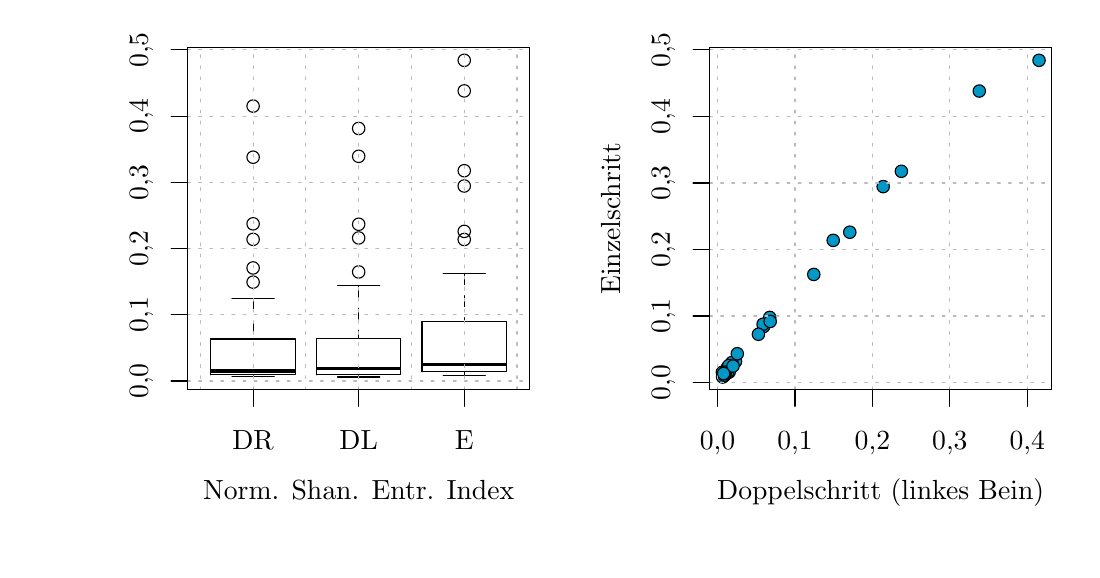
\begin{tikzpicture}[x=1pt,y=1pt]
\definecolor{fillColor}{RGB}{255,255,255}
\path[use as bounding box,fill=fillColor,fill opacity=0.00] (0,0) rectangle (377.25,188.62);
\begin{scope}
\path[clip] ( 57.82, 57.82) rectangle (181.40,181.40);
\definecolor{drawColor}{RGB}{0,0,0}

\path[draw=drawColor,line width= 1.2pt,line join=round] ( 66.21, 64.53) -- ( 96.72, 64.53);

\path[draw=drawColor,line width= 0.4pt,dash pattern=on 4pt off 4pt ,line join=round,line cap=round] ( 81.46, 62.42) -- ( 81.46, 63.18);

\path[draw=drawColor,line width= 0.4pt,dash pattern=on 4pt off 4pt ,line join=round,line cap=round] ( 81.46, 90.67) -- ( 81.46, 76.12);

\path[draw=drawColor,line width= 0.4pt,line join=round,line cap=round] ( 73.84, 62.42) -- ( 89.09, 62.42);

\path[draw=drawColor,line width= 0.4pt,line join=round,line cap=round] ( 73.84, 90.67) -- ( 89.09, 90.67);

\path[draw=drawColor,line width= 0.4pt,line join=round,line cap=round] ( 66.21, 63.18) --
	( 96.72, 63.18) --
	( 96.72, 76.12) --
	( 66.21, 76.12) --
	( 66.21, 63.18);

\path[draw=drawColor,line width= 0.4pt,line join=round,line cap=round] ( 81.46,101.80) circle (  2.25);

\path[draw=drawColor,line width= 0.4pt,line join=round,line cap=round] ( 81.46, 96.67) circle (  2.25);

\path[draw=drawColor,line width= 0.4pt,line join=round,line cap=round] ( 81.46,112.12) circle (  2.25);

\path[draw=drawColor,line width= 0.4pt,line join=round,line cap=round] ( 81.46,141.81) circle (  2.25);

\path[draw=drawColor,line width= 0.4pt,line join=round,line cap=round] ( 81.46,160.28) circle (  2.25);

\path[draw=drawColor,line width= 0.4pt,line join=round,line cap=round] ( 81.46,117.74) circle (  2.25);

\path[draw=drawColor,line width= 1.2pt,line join=round] (104.35, 65.35) -- (134.86, 65.35);

\path[draw=drawColor,line width= 0.4pt,dash pattern=on 4pt off 4pt ,line join=round,line cap=round] (119.61, 62.39) -- (119.61, 63.14);

\path[draw=drawColor,line width= 0.4pt,dash pattern=on 4pt off 4pt ,line join=round,line cap=round] (119.61, 95.30) -- (119.61, 76.40);

\path[draw=drawColor,line width= 0.4pt,line join=round,line cap=round] (111.98, 62.39) -- (127.24, 62.39);

\path[draw=drawColor,line width= 0.4pt,line join=round,line cap=round] (111.98, 95.30) -- (127.24, 95.30);

\path[draw=drawColor,line width= 0.4pt,line join=round,line cap=round] (104.35, 63.14) --
	(134.86, 63.14) --
	(134.86, 76.40) --
	(104.35, 76.40) --
	(104.35, 63.14);

\path[draw=drawColor,line width= 0.4pt,line join=round,line cap=round] (119.61,100.35) circle (  2.25);

\path[draw=drawColor,line width= 0.4pt,line join=round,line cap=round] (119.61,112.64) circle (  2.25);

\path[draw=drawColor,line width= 0.4pt,line join=round,line cap=round] (119.61,142.14) circle (  2.25);

\path[draw=drawColor,line width= 0.4pt,line join=round,line cap=round] (119.61,152.20) circle (  2.25);

\path[draw=drawColor,line width= 0.4pt,line join=round,line cap=round] (119.61,117.58) circle (  2.25);

\path[draw=drawColor,line width= 1.2pt,line join=round] (142.49, 66.86) -- (173.01, 66.86);

\path[draw=drawColor,line width= 0.4pt,dash pattern=on 4pt off 4pt ,line join=round,line cap=round] (157.75, 62.95) -- (157.75, 64.28);

\path[draw=drawColor,line width= 0.4pt,dash pattern=on 4pt off 4pt ,line join=round,line cap=round] (157.75, 99.82) -- (157.75, 82.43);

\path[draw=drawColor,line width= 0.4pt,line join=round,line cap=round] (150.12, 62.95) -- (165.38, 62.95);

\path[draw=drawColor,line width= 0.4pt,line join=round,line cap=round] (150.12, 99.82) -- (165.38, 99.82);

\path[draw=drawColor,line width= 0.4pt,line join=round,line cap=round] (142.49, 64.28) --
	(173.01, 64.28) --
	(173.01, 82.43) --
	(142.49, 82.43) --
	(142.49, 64.28);

\path[draw=drawColor,line width= 0.4pt,line join=round,line cap=round] (157.75,115.01) circle (  2.25);

\path[draw=drawColor,line width= 0.4pt,line join=round,line cap=round] (157.75,112.08) circle (  2.25);

\path[draw=drawColor,line width= 0.4pt,line join=round,line cap=round] (157.75,131.41) circle (  2.25);

\path[draw=drawColor,line width= 0.4pt,line join=round,line cap=round] (157.75,165.77) circle (  2.25);

\path[draw=drawColor,line width= 0.4pt,line join=round,line cap=round] (157.75,176.82) circle (  2.25);

\path[draw=drawColor,line width= 0.4pt,line join=round,line cap=round] (157.75,136.93) circle (  2.25);
\end{scope}
\begin{scope}
\path[clip] (  0.00,  0.00) rectangle (377.25,188.62);
\definecolor{drawColor}{RGB}{0,0,0}

\path[draw=drawColor,line width= 0.4pt,line join=round,line cap=round] ( 81.46, 57.82) -- (157.75, 57.82);

\path[draw=drawColor,line width= 0.4pt,line join=round,line cap=round] ( 81.46, 57.82) -- ( 81.46, 51.82);

\path[draw=drawColor,line width= 0.4pt,line join=round,line cap=round] (119.61, 57.82) -- (119.61, 51.82);

\path[draw=drawColor,line width= 0.4pt,line join=round,line cap=round] (157.75, 57.82) -- (157.75, 51.82);

\node[text=drawColor,anchor=base,inner sep=0pt, outer sep=0pt, scale=  1.00] at ( 81.46, 36.22) {DR};

\node[text=drawColor,anchor=base,inner sep=0pt, outer sep=0pt, scale=  1.00] at (119.61, 36.22) {DL};

\node[text=drawColor,anchor=base,inner sep=0pt, outer sep=0pt, scale=  1.00] at (157.75, 36.22) {E};

\path[draw=drawColor,line width= 0.4pt,line join=round,line cap=round] ( 57.82, 60.94) -- ( 57.82,180.58);

\path[draw=drawColor,line width= 0.4pt,line join=round,line cap=round] ( 57.82, 60.94) -- ( 51.82, 60.94);

\path[draw=drawColor,line width= 0.4pt,line join=round,line cap=round] ( 57.82, 84.87) -- ( 51.82, 84.87);

\path[draw=drawColor,line width= 0.4pt,line join=round,line cap=round] ( 57.82,108.80) -- ( 51.82,108.80);

\path[draw=drawColor,line width= 0.4pt,line join=round,line cap=round] ( 57.82,132.72) -- ( 51.82,132.72);

\path[draw=drawColor,line width= 0.4pt,line join=round,line cap=round] ( 57.82,156.65) -- ( 51.82,156.65);

\path[draw=drawColor,line width= 0.4pt,line join=round,line cap=round] ( 57.82,180.58) -- ( 51.82,180.58);

\node[text=drawColor,rotate= 90.00,anchor=base,inner sep=0pt, outer sep=0pt, scale=  1.00] at ( 43.42, 60.94) {0,0};

\node[text=drawColor,rotate= 90.00,anchor=base,inner sep=0pt, outer sep=0pt, scale=  1.00] at ( 43.42, 84.87) {0,1};

\node[text=drawColor,rotate= 90.00,anchor=base,inner sep=0pt, outer sep=0pt, scale=  1.00] at ( 43.42,108.80) {0,2};

\node[text=drawColor,rotate= 90.00,anchor=base,inner sep=0pt, outer sep=0pt, scale=  1.00] at ( 43.42,132.72) {0,3};

\node[text=drawColor,rotate= 90.00,anchor=base,inner sep=0pt, outer sep=0pt, scale=  1.00] at ( 43.42,156.65) {0,4};

\node[text=drawColor,rotate= 90.00,anchor=base,inner sep=0pt, outer sep=0pt, scale=  1.00] at ( 43.42,180.58) {0,5};
\end{scope}
\begin{scope}
\path[clip] (  0.00,  0.00) rectangle (188.62,188.62);
\definecolor{drawColor}{RGB}{0,0,0}

\node[text=drawColor,anchor=base,inner sep=0pt, outer sep=0pt, scale=  1.00] at (119.61, 18.22) {Norm. Shan. Entr. Index};
\end{scope}
\begin{scope}
\path[clip] (  0.00,  0.00) rectangle (377.25,188.62);
\definecolor{drawColor}{RGB}{0,0,0}

\path[draw=drawColor,line width= 0.4pt,line join=round,line cap=round] ( 57.82, 57.82) --
	(181.40, 57.82) --
	(181.40,181.40) --
	( 57.82,181.40) --
	( 57.82, 57.82);
\end{scope}
\begin{scope}
\path[clip] ( 57.82, 57.82) rectangle (181.40,181.40);
\definecolor{drawColor}{RGB}{186,187,194}

\path[draw=drawColor,line width= 0.4pt,dash pattern=on 1pt off 3pt ,line join=round,line cap=round] ( 62.39, 57.82) -- ( 62.39,181.40);

\path[draw=drawColor,line width= 0.4pt,dash pattern=on 1pt off 3pt ,line join=round,line cap=round] ( 81.46, 57.82) -- ( 81.46,181.40);

\path[draw=drawColor,line width= 0.4pt,dash pattern=on 1pt off 3pt ,line join=round,line cap=round] (100.54, 57.82) -- (100.54,181.40);

\path[draw=drawColor,line width= 0.4pt,dash pattern=on 1pt off 3pt ,line join=round,line cap=round] (119.61, 57.82) -- (119.61,181.40);

\path[draw=drawColor,line width= 0.4pt,dash pattern=on 1pt off 3pt ,line join=round,line cap=round] (138.68, 57.82) -- (138.68,181.40);

\path[draw=drawColor,line width= 0.4pt,dash pattern=on 1pt off 3pt ,line join=round,line cap=round] (157.75, 57.82) -- (157.75,181.40);

\path[draw=drawColor,line width= 0.4pt,dash pattern=on 1pt off 3pt ,line join=round,line cap=round] (176.82, 57.82) -- (176.82,181.40);

\path[draw=drawColor,line width= 0.4pt,dash pattern=on 1pt off 3pt ,line join=round,line cap=round] ( 57.82, 60.94) -- (181.40, 60.94);

\path[draw=drawColor,line width= 0.4pt,dash pattern=on 1pt off 3pt ,line join=round,line cap=round] ( 57.82, 84.87) -- (181.40, 84.87);

\path[draw=drawColor,line width= 0.4pt,dash pattern=on 1pt off 3pt ,line join=round,line cap=round] ( 57.82,108.80) -- (181.40,108.80);

\path[draw=drawColor,line width= 0.4pt,dash pattern=on 1pt off 3pt ,line join=round,line cap=round] ( 57.82,132.72) -- (181.40,132.72);

\path[draw=drawColor,line width= 0.4pt,dash pattern=on 1pt off 3pt ,line join=round,line cap=round] ( 57.82,156.65) -- (181.40,156.65);

\path[draw=drawColor,line width= 0.4pt,dash pattern=on 1pt off 3pt ,line join=round,line cap=round] ( 57.82,180.58) -- (181.40,180.58);
\end{scope}
\begin{scope}
\path[clip] (  0.00,  0.00) rectangle (377.25,188.62);
\definecolor{drawColor}{RGB}{0,0,0}

\path[draw=drawColor,line width= 0.4pt,line join=round,line cap=round] ( 57.82, 57.82) --
	(181.40, 57.82) --
	(181.40,181.40) --
	( 57.82,181.40) --
	( 57.82, 57.82);
\end{scope}
\begin{scope}
\path[clip] (246.44, 57.82) rectangle (370.02,181.40);
\definecolor{drawColor}{RGB}{0,0,0}
\definecolor{fillColor}{RGB}{0,152,199}

\path[draw=drawColor,line width= 0.4pt,line join=round,line cap=round,fill=fillColor] (251.95, 63.42) circle (  2.25);

\path[draw=drawColor,line width= 0.4pt,line join=round,line cap=round,fill=fillColor] (297.07,114.71) circle (  2.25);

\path[draw=drawColor,line width= 0.4pt,line join=round,line cap=round,fill=fillColor] (252.61, 64.42) circle (  2.25);

\path[draw=drawColor,line width= 0.4pt,line join=round,line cap=round,fill=fillColor] (253.49, 64.20) circle (  2.25);

\path[draw=drawColor,line width= 0.4pt,line join=round,line cap=round,fill=fillColor] (255.77, 67.97) circle (  2.25);

\path[draw=drawColor,line width= 0.4pt,line join=round,line cap=round,fill=fillColor] (268.14, 83.92) circle (  2.25);

\path[draw=drawColor,line width= 0.4pt,line join=round,line cap=round,fill=fillColor] (291.07,111.76) circle (  2.25);

\path[draw=drawColor,line width= 0.4pt,line join=round,line cap=round,fill=fillColor] (284.06, 99.45) circle (  2.25);

\path[draw=drawColor,line width= 0.4pt,line join=round,line cap=round,fill=fillColor] (251.23, 62.88) circle (  2.25);

\path[draw=drawColor,line width= 0.4pt,line join=round,line cap=round,fill=fillColor] (251.59, 62.77) circle (  2.25);

\path[draw=drawColor,line width= 0.4pt,line join=round,line cap=round,fill=fillColor] (309.14,131.19) circle (  2.25);

\path[draw=drawColor,line width= 0.4pt,line join=round,line cap=round,fill=fillColor] (265.94, 80.62) circle (  2.25);

\path[draw=drawColor,line width= 0.4pt,line join=round,line cap=round,fill=fillColor] (265.75, 81.47) circle (  2.25);

\path[draw=drawColor,line width= 0.4pt,line join=round,line cap=round,fill=fillColor] (268.30, 82.47) circle (  2.25);

\path[draw=drawColor,line width= 0.4pt,line join=round,line cap=round,fill=fillColor] (252.57, 64.58) circle (  2.25);

\path[draw=drawColor,line width= 0.4pt,line join=round,line cap=round,fill=fillColor] (264.06, 77.83) circle (  2.25);

\path[draw=drawColor,line width= 0.4pt,line join=round,line cap=round,fill=fillColor] (251.40, 63.20) circle (  2.25);

\path[draw=drawColor,line width= 0.4pt,line join=round,line cap=round,fill=fillColor] (254.48, 67.17) circle (  2.25);

\path[draw=drawColor,line width= 0.4pt,line join=round,line cap=round,fill=fillColor] (252.80, 63.85) circle (  2.25);

\path[draw=drawColor,line width= 0.4pt,line join=round,line cap=round,fill=fillColor] (343.86,165.72) circle (  2.25);

\path[draw=drawColor,line width= 0.4pt,line join=round,line cap=round,fill=fillColor] (251.13, 62.39) circle (  2.25);

\path[draw=drawColor,line width= 0.4pt,line join=round,line cap=round,fill=fillColor] (251.87, 63.83) circle (  2.25);

\path[draw=drawColor,line width= 0.4pt,line join=round,line cap=round,fill=fillColor] (365.45,176.82) circle (  2.25);

\path[draw=drawColor,line width= 0.4pt,line join=round,line cap=round,fill=fillColor] (254.42, 67.58) circle (  2.25);

\path[draw=drawColor,line width= 0.4pt,line join=round,line cap=round,fill=fillColor] (315.71,136.73) circle (  2.25);

\path[draw=drawColor,line width= 0.4pt,line join=round,line cap=round,fill=fillColor] (251.98, 63.17) circle (  2.25);

\path[draw=drawColor,line width= 0.4pt,line join=round,line cap=round,fill=fillColor] (251.02, 64.11) circle (  2.25);

\path[draw=drawColor,line width= 0.4pt,line join=round,line cap=round,fill=fillColor] (252.87, 65.82) circle (  2.25);

\path[draw=drawColor,line width= 0.4pt,line join=round,line cap=round,fill=fillColor] (253.38, 66.54) circle (  2.25);

\path[draw=drawColor,line width= 0.4pt,line join=round,line cap=round,fill=fillColor] (252.09, 64.14) circle (  2.25);

\path[draw=drawColor,line width= 0.4pt,line join=round,line cap=round,fill=fillColor] (251.70, 63.04) circle (  2.25);

\path[draw=drawColor,line width= 0.4pt,line join=round,line cap=round,fill=fillColor] (251.77, 63.59) circle (  2.25);

\path[draw=drawColor,line width= 0.4pt,line join=round,line cap=round,fill=fillColor] (254.88, 66.33) circle (  2.25);

\path[draw=drawColor,line width= 0.4pt,line join=round,line cap=round,fill=fillColor] (251.47, 63.63) circle (  2.25);

\path[draw=drawColor,line width= 0.4pt,line join=round,line cap=round,fill=fillColor] (256.42, 70.80) circle (  2.25);
\end{scope}
\begin{scope}
\path[clip] (  0.00,  0.00) rectangle (377.25,188.62);
\definecolor{drawColor}{RGB}{0,0,0}

\path[draw=drawColor,line width= 0.4pt,line join=round,line cap=round] (249.30, 57.82) -- (361.21, 57.82);

\path[draw=drawColor,line width= 0.4pt,line join=round,line cap=round] (249.30, 57.82) -- (249.30, 51.82);

\path[draw=drawColor,line width= 0.4pt,line join=round,line cap=round] (277.27, 57.82) -- (277.27, 51.82);

\path[draw=drawColor,line width= 0.4pt,line join=round,line cap=round] (305.25, 57.82) -- (305.25, 51.82);

\path[draw=drawColor,line width= 0.4pt,line join=round,line cap=round] (333.23, 57.82) -- (333.23, 51.82);

\path[draw=drawColor,line width= 0.4pt,line join=round,line cap=round] (361.21, 57.82) -- (361.21, 51.82);

\node[text=drawColor,anchor=base,inner sep=0pt, outer sep=0pt, scale=  1.00] at (249.30, 36.22) {0,0};

\node[text=drawColor,anchor=base,inner sep=0pt, outer sep=0pt, scale=  1.00] at (277.27, 36.22) {0,1};

\node[text=drawColor,anchor=base,inner sep=0pt, outer sep=0pt, scale=  1.00] at (305.25, 36.22) {0,2};

\node[text=drawColor,anchor=base,inner sep=0pt, outer sep=0pt, scale=  1.00] at (333.23, 36.22) {0,3};

\node[text=drawColor,anchor=base,inner sep=0pt, outer sep=0pt, scale=  1.00] at (361.21, 36.22) {0,4};

\path[draw=drawColor,line width= 0.4pt,line join=round,line cap=round] (246.44, 60.38) -- (246.44,180.60);

\path[draw=drawColor,line width= 0.4pt,line join=round,line cap=round] (246.44, 60.38) -- (240.44, 60.38);

\path[draw=drawColor,line width= 0.4pt,line join=round,line cap=round] (246.44, 84.42) -- (240.44, 84.42);

\path[draw=drawColor,line width= 0.4pt,line join=round,line cap=round] (246.44,108.46) -- (240.44,108.46);

\path[draw=drawColor,line width= 0.4pt,line join=round,line cap=round] (246.44,132.51) -- (240.44,132.51);

\path[draw=drawColor,line width= 0.4pt,line join=round,line cap=round] (246.44,156.55) -- (240.44,156.55);

\path[draw=drawColor,line width= 0.4pt,line join=round,line cap=round] (246.44,180.60) -- (240.44,180.60);

\node[text=drawColor,rotate= 90.00,anchor=base,inner sep=0pt, outer sep=0pt, scale=  1.00] at (232.04, 60.38) {0,0};

\node[text=drawColor,rotate= 90.00,anchor=base,inner sep=0pt, outer sep=0pt, scale=  1.00] at (232.04, 84.42) {0,1};

\node[text=drawColor,rotate= 90.00,anchor=base,inner sep=0pt, outer sep=0pt, scale=  1.00] at (232.04,108.46) {0,2};

\node[text=drawColor,rotate= 90.00,anchor=base,inner sep=0pt, outer sep=0pt, scale=  1.00] at (232.04,132.51) {0,3};

\node[text=drawColor,rotate= 90.00,anchor=base,inner sep=0pt, outer sep=0pt, scale=  1.00] at (232.04,156.55) {0,4};

\node[text=drawColor,rotate= 90.00,anchor=base,inner sep=0pt, outer sep=0pt, scale=  1.00] at (232.04,180.60) {0,5};

\path[draw=drawColor,line width= 0.4pt,line join=round,line cap=round] (246.44, 57.82) --
	(370.02, 57.82) --
	(370.02,181.40) --
	(246.44,181.40) --
	(246.44, 57.82);
\end{scope}
\begin{scope}
\path[clip] (188.62,  0.00) rectangle (377.25,188.62);
\definecolor{drawColor}{RGB}{0,0,0}

\node[text=drawColor,anchor=base,inner sep=0pt, outer sep=0pt, scale=  1.00] at (308.23, 18.22) {Doppelschritt (linkes Bein)};

\node[text=drawColor,rotate= 90.00,anchor=base,inner sep=0pt, outer sep=0pt, scale=  1.00] at (214.04,119.61) {Einzelschritt};
\end{scope}
\begin{scope}
\path[clip] (246.44, 57.82) rectangle (370.02,181.40);
\definecolor{drawColor}{RGB}{186,187,194}

\path[draw=drawColor,line width= 0.4pt,dash pattern=on 1pt off 3pt ,line join=round,line cap=round] (249.30, 57.82) -- (249.30,181.40);

\path[draw=drawColor,line width= 0.4pt,dash pattern=on 1pt off 3pt ,line join=round,line cap=round] (277.27, 57.82) -- (277.27,181.40);

\path[draw=drawColor,line width= 0.4pt,dash pattern=on 1pt off 3pt ,line join=round,line cap=round] (305.25, 57.82) -- (305.25,181.40);

\path[draw=drawColor,line width= 0.4pt,dash pattern=on 1pt off 3pt ,line join=round,line cap=round] (333.23, 57.82) -- (333.23,181.40);

\path[draw=drawColor,line width= 0.4pt,dash pattern=on 1pt off 3pt ,line join=round,line cap=round] (361.21, 57.82) -- (361.21,181.40);

\path[draw=drawColor,line width= 0.4pt,dash pattern=on 1pt off 3pt ,line join=round,line cap=round] (246.44, 60.38) -- (370.02, 60.38);

\path[draw=drawColor,line width= 0.4pt,dash pattern=on 1pt off 3pt ,line join=round,line cap=round] (246.44, 84.42) -- (370.02, 84.42);

\path[draw=drawColor,line width= 0.4pt,dash pattern=on 1pt off 3pt ,line join=round,line cap=round] (246.44,108.46) -- (370.02,108.46);

\path[draw=drawColor,line width= 0.4pt,dash pattern=on 1pt off 3pt ,line join=round,line cap=round] (246.44,132.51) -- (370.02,132.51);

\path[draw=drawColor,line width= 0.4pt,dash pattern=on 1pt off 3pt ,line join=round,line cap=round] (246.44,156.55) -- (370.02,156.55);

\path[draw=drawColor,line width= 0.4pt,dash pattern=on 1pt off 3pt ,line join=round,line cap=round] (246.44,180.60) -- (370.02,180.60);
\end{scope}
\begin{scope}
\path[clip] (  0.00,  0.00) rectangle (377.25,188.62);
\definecolor{drawColor}{RGB}{0,0,0}

\path[draw=drawColor,line width= 0.4pt,line join=round,line cap=round] (246.44, 57.82) --
	(370.02, 57.82) --
	(370.02,181.40) --
	(246.44,181.40) --
	(246.44, 57.82);
\end{scope}
\end{tikzpicture}
 \caption[Kardio-lokomotorischen Phasensynchronation: Vergleich der Doppelschrittberechnung und Einzelschrittberechnung.]{Kardio-lokomotorischen Phasensynchronation: Vergleich der Doppelschrittberechnung und Einzelschrittberechnung: (rechts) Mittelwertvergleich; (links) Zusammenhang zwischen Doppelschrittberechnung ausgehend vom linken Bein und Einzelschrittberechnung. \emph{Anmerkung}: \\
	\hspace{
	\textwidth}DL = Doppelschrittberechnung ausgehend vom linken Bein \\
	\hspace{
	\textwidth}DR = Doppelschrittberechnung ausgehend vom rechten Bein \\
	\hspace{
	\textwidth}E = Einzelschritt} \label{fig:index_vergleich} 
\end{figure}

% subsection operationalisierung_und_gewonnene_daten (end)
\subsection{Ergebnisse} 

% (fold)
\label{sub:ergebnisse_5_3}

\subsubsection{Korrelationsanalyse} 

% (fold)
\label{ssub:korrelationsanalyse_5_3}

Ich führte eine bivariate Korrelationsanalyse durch, um Zusammenhänge zwischen den Merkmalen der \ac{FKS}, der kardio-lokomorischen Phasensynchronisation und dem Bewegungsaufwand zu finden. Die Korrelationkoeffizienten sind in der Korrelationsmatrix in Tabelle~\ref{tab:korrelationen_3} dargestellt. Bei der Berechnung ließ ich die Bedingung der Normalverteilung (nötig für die exakte Abschätzung der Signifikanz) bei den impliziten Merkmalen mittlere HR und mittlerem normalisierten Shannon Entropie Index unberücksichtig. Die Korrelationsmatrix zeigt die signifikanten Zusammenhänge zwischen Generalfaktor und seiner beiden Dimensionen \emph{glatter Verlauf} und \emph{Absorbiertheit}. Zusätzlich korrelieren beide Dimensionen positiv. Ein weiterer linear positiver Zusammenhang wurde zwischen den beiden nicht normalverteilten impliziten Merkmalen mittlere HR HR und mittlerem normalisierten Shannon Entropie Index festgestellt.

Zwischen den impliziten Merkmalen (mittlere HR, mittlerer normalisierter Shannon Entropie Index, mittlerer Doppelschrittfrequenz und Bewegungsaufwand) und den explizit erhobenen Flow-Merkmalen konnte ich keine lineare Zusammenhänge feststellen.
\begin{sidewaystable}
	\centering \caption[Korrelationsmatrix (Finale Studie: Laufen).]{Korrelationsmatrix der finalen Studie zum Flow-Erleben beim Laufen: Arithmetisches Mittel, Standardabweichung und Korrelationen. \\
	\hspace{
	\textwidth}\emph{Anmerkung}: Bew. = Bewegungsaufwand \\
	\hspace{
	\textwidth}* Korrelation ist auf dem Niveau von 0,05 (zweiseitig) signifikant \\
	\hspace{
	\textwidth}** Korrelation ist auf dem Niveau von 0,01 (zweiseitig) signifikant} \label{tab:korrelationen_3} 
	\begin{tabular}
		{lxxxxxxxx} \toprule & M & SD & 1 & 2 & 3 & 4 & 5 & 6 \\
		\midrule 1. Generalfaktor & 4,85 & 0,79 & & & & & & \\
		2. Glatter Verlauf & 4,86 & 0,95 & 0,92** & & & & & \\
		3. Absorbiertheit & 4,85 & 0,87 & 0,78** & 0,47** & & & & \\
		4. HR ($1/min$) & 166,36 & 14,53 & 0,12 & 0,02 & 0,24 & & & \\
		5. Norm. Shan. Entr. Index & 0,09 & 0,13 & 0,29 & 0,18 & 0,36* & -0,04 & & \\
		6. Doppelschrittfrequenz ($1/min$) rechts & 82,68 & 4,86 & 0,29 & 0,22 & 0,29 & 0,21 & 0,02 & \\
		7. Bew. ($\times 10^3 \: m^2 \cdot s^{-5}$) rechts & 33,21 & 4,60 & -0,10 & 0,03 & -0,28 & 0,33 & -0,16 & 0,28 \\
		\bottomrule 
	\end{tabular}
\end{sidewaystable}

Damit kann ich keinen direkten Zusammenhang von Flow-Erleben und kardio-lokomotorischer Phasensychronisation feststellen (Abschnitt~\ref{sub:hypothesen}, $H^1$). Aus diesem Grund testete ich im nächsten Schritt den Effekt einer \emph{physiologisch gemessenen \ac{AFP}} auf das Flow-Erleben (Abschnitt~\ref{sub:hypothesen}, $H^2$).

% subsubsection korrelationsanalyse (end)
\subsubsection{Effekt der physiologisch gemessenen \ac{AFP} auf das Flow-Erleben} 

% (fold)
\label{ssub:effekt_der_physiologisch_gemessenen_afp}

In dieser Effektuntersuchung unterteilte ich die gemessenen expliziten Merkmale der Untersuchungspersonen in drei Gruppen auf. Bei sieben Untersuchungspersonen konnte ich in einen Zeitabschnitt von 15 Minuten vor der Befragung zumindenstens teilweise eine kardio-lokomotorische Phasensynchronisation feststellen (Gruppe: \emph{Gleichgewicht}). Bei den restlichen 22 Untersuchungsperson stellte ich bei zehn Untersuchungspersonenen eine höhere mittlere Schrittfrequenz als mittlere HR fest (Gruppe: \emph{Schritt dominiert}) und bei 14 Untersuchungspersonenen eine niedrigere mittlere Schrittfrequenz als mittlere HR fest (Gruppe: \emph{Herz dominiert}).

In der Analyse untersuchte ich, ob die Gruppe \emph{Gleichgewicht} mehr Flow-Erleben, gemessen am Generalfaktor der \ac{FKS}, erlebte als die Gruppe \emph{Schritt dominiert} oder die Gruppe \emph{Herz dominiert}. Als Methode nutzte ich einen Zweistichproben t-Test für unabhängige Stichproben ein. Der Zweistichproben t-Test setzt eine Normalverteilung der beiden zu testenen Stichproben und eine Varianzhomogenität (Gleichheit der Varianzen der beiden Stichproben) voraus. Bei allen nachflogenen Ergebnissen wurden diese Voraussetzungen nicht verletzt. 

In der Gruppe \emph{Gleichgewicht} beobachtete ich höhere Werte des Generalfaktors ($M = 4{,}73; SD = 0{,}69$) als in der Gruppe \emph{Schritt dominiert} ($M = 5{,}37; SD = 0{,}87$) oder in der Gruppe \emph{Herz dominiert} ($M = 4{,}69; SD = 0{,}76$) (Abbildung~\ref{fig:mittelwert_vergleich}, A). 
\begin{itemize}
	
	\item Beide Unterschiede konnte ich nicht als signifikant nachweisen, $t(19) = 1{,}85; p < 0{,}1$ und $t(15) = 1{,}69; p = 0{,}11$.
\end{itemize}

Daraufhin testete ich die beiden Subdimension der \ac{FKS}. Auch beim Glatten Verlauf sind in der Gruppe \emph{Gleichgewicht} höhere Werte zu beobachten ($M = 5{,}24; SD = 0{,}92$) als in der Gruppe \emph{Schritt dominiert} ($M = 4{,}81; SD = 0{,}8$) oder in der Gruppe \emph{Herz dominiert} ($M = 4{,}7; SD = 1{,}1$) (Abbildung~\ref{fig:mittelwert_vergleich}, B). 

Gleiches gilt für die Absorbiertheit. Die Gruppe \emph{Gleichgewicht} höhere Werte ($M = 5{,}57; SD = 0{,}87$) als die Gruppe \emph{Schritt dominiert} ($M = 4{,}6; SD = 0{,}84$) oder die Gruppe \emph{Herz dominiert} ($M = 4{,}66; SD = 0{,}74$) (Abbildung~\ref{fig:mittelwert_vergleich}, C)
\begin{itemize}
	
	\item Die Unterschiede für den glatten Verlauf sind nicht signifikant, $t(19) = 1{,}13; p = 0{,}27$ und $t(15) = 1{,}0; p = 0{,}33$.
	
	\item Für beide Unterschiede bei der Absorbiertheit konnte ich eine \emph{Signifikanz nachweisen}, $t(19) = 2{,}5; p < 0{,}05$ und $t(15) = 2{,}3; p < 0{,}05$.
\end{itemize}
\begin{figure}
	[thb!] % Created by tikzDevice version 0.10.1 on 2016-09-12 13:47:03
% !TEX encoding = UTF-8 Unicode
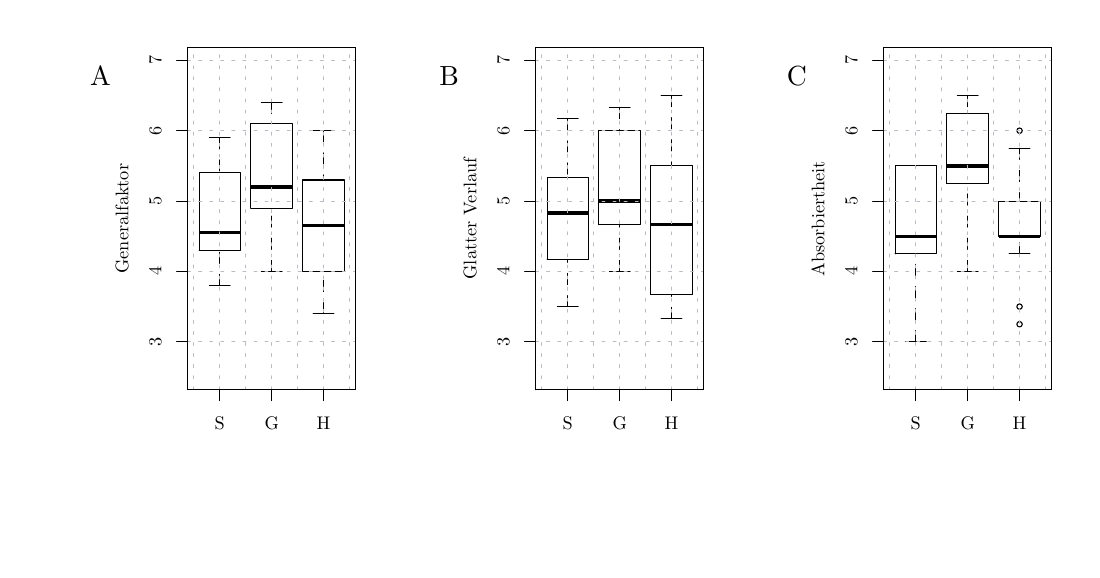
\begin{tikzpicture}[x=1pt,y=1pt]
\definecolor{fillColor}{RGB}{255,255,255}
\path[use as bounding box,fill=fillColor,fill opacity=0.00] (0,0) rectangle (377.25,188.62);
\begin{scope}
\path[clip] ( 57.82, 57.82) rectangle (118.52,181.40);
\definecolor{drawColor}{RGB}{0,0,0}

\path[draw=drawColor,line width= 1.2pt,line join=round] ( 61.94,114.52) -- ( 76.93,114.52);

\path[draw=drawColor,line width= 0.4pt,dash pattern=on 4pt off 4pt ,line join=round,line cap=round] ( 69.43, 95.45) -- ( 69.43,108.16);

\path[draw=drawColor,line width= 0.4pt,dash pattern=on 4pt off 4pt ,line join=round,line cap=round] ( 69.43,148.85) -- ( 69.43,136.14);

\path[draw=drawColor,line width= 0.4pt,line join=round,line cap=round] ( 65.69, 95.45) -- ( 73.18, 95.45);

\path[draw=drawColor,line width= 0.4pt,line join=round,line cap=round] ( 65.69,148.85) -- ( 73.18,148.85);

\path[draw=drawColor,line width= 0.4pt,line join=round,line cap=round] ( 61.94,108.16) --
	( 76.93,108.16) --
	( 76.93,136.14) --
	( 61.94,136.14) --
	( 61.94,108.16);

\path[draw=drawColor,line width= 1.2pt,line join=round] ( 80.67,131.05) -- ( 95.66,131.05);

\path[draw=drawColor,line width= 0.4pt,dash pattern=on 4pt off 4pt ,line join=round,line cap=round] ( 88.17,100.54) -- ( 88.17,123.42);

\path[draw=drawColor,line width= 0.4pt,dash pattern=on 4pt off 4pt ,line join=round,line cap=round] ( 88.17,161.56) -- ( 88.17,153.94);

\path[draw=drawColor,line width= 0.4pt,line join=round,line cap=round] ( 84.42,100.54) -- ( 91.92,100.54);

\path[draw=drawColor,line width= 0.4pt,line join=round,line cap=round] ( 84.42,161.56) -- ( 91.92,161.56);

\path[draw=drawColor,line width= 0.4pt,line join=round,line cap=round] ( 80.67,123.42) --
	( 95.66,123.42) --
	( 95.66,153.94) --
	( 80.67,153.94) --
	( 80.67,123.42);

\path[draw=drawColor,line width= 1.2pt,line join=round] ( 99.41,117.06) -- (114.40,117.06);

\path[draw=drawColor,line width= 0.4pt,dash pattern=on 4pt off 4pt ,line join=round,line cap=round] (106.91, 85.28) -- (106.91,100.54);

\path[draw=drawColor,line width= 0.4pt,dash pattern=on 4pt off 4pt ,line join=round,line cap=round] (106.91,151.39) -- (106.91,133.59);

\path[draw=drawColor,line width= 0.4pt,line join=round,line cap=round] (103.16, 85.28) -- (110.65, 85.28);

\path[draw=drawColor,line width= 0.4pt,line join=round,line cap=round] (103.16,151.39) -- (110.65,151.39);

\path[draw=drawColor,line width= 0.4pt,line join=round,line cap=round] ( 99.41,100.54) --
	(114.40,100.54) --
	(114.40,133.59) --
	( 99.41,133.59) --
	( 99.41,100.54);
\end{scope}
\begin{scope}
\path[clip] (  0.00,  0.00) rectangle (377.25,188.62);
\definecolor{drawColor}{RGB}{0,0,0}

\path[draw=drawColor,line width= 0.4pt,line join=round,line cap=round] ( 69.43, 57.82) -- (106.91, 57.82);

\path[draw=drawColor,line width= 0.4pt,line join=round,line cap=round] ( 69.43, 57.82) -- ( 69.43, 53.86);

\path[draw=drawColor,line width= 0.4pt,line join=round,line cap=round] ( 88.17, 57.82) -- ( 88.17, 53.86);

\path[draw=drawColor,line width= 0.4pt,line join=round,line cap=round] (106.91, 57.82) -- (106.91, 53.86);

\node[text=drawColor,anchor=base,inner sep=0pt, outer sep=0pt, scale=  0.66] at ( 69.43, 43.56) {S};

\node[text=drawColor,anchor=base,inner sep=0pt, outer sep=0pt, scale=  0.66] at ( 88.17, 43.56) {G};

\node[text=drawColor,anchor=base,inner sep=0pt, outer sep=0pt, scale=  0.66] at (106.91, 43.56) {H};

\path[draw=drawColor,line width= 0.4pt,line join=round,line cap=round] ( 57.82, 75.11) -- ( 57.82,176.82);

\path[draw=drawColor,line width= 0.4pt,line join=round,line cap=round] ( 57.82, 75.11) -- ( 53.86, 75.11);

\path[draw=drawColor,line width= 0.4pt,line join=round,line cap=round] ( 57.82,100.54) -- ( 53.86,100.54);

\path[draw=drawColor,line width= 0.4pt,line join=round,line cap=round] ( 57.82,125.96) -- ( 53.86,125.96);

\path[draw=drawColor,line width= 0.4pt,line join=round,line cap=round] ( 57.82,151.39) -- ( 53.86,151.39);

\path[draw=drawColor,line width= 0.4pt,line join=round,line cap=round] ( 57.82,176.82) -- ( 53.86,176.82);

\node[text=drawColor,rotate= 90.00,anchor=base,inner sep=0pt, outer sep=0pt, scale=  0.66] at ( 48.31, 75.11) {3};

\node[text=drawColor,rotate= 90.00,anchor=base,inner sep=0pt, outer sep=0pt, scale=  0.66] at ( 48.31,100.54) {4};

\node[text=drawColor,rotate= 90.00,anchor=base,inner sep=0pt, outer sep=0pt, scale=  0.66] at ( 48.31,125.96) {5};

\node[text=drawColor,rotate= 90.00,anchor=base,inner sep=0pt, outer sep=0pt, scale=  0.66] at ( 48.31,151.39) {6};

\node[text=drawColor,rotate= 90.00,anchor=base,inner sep=0pt, outer sep=0pt, scale=  0.66] at ( 48.31,176.82) {7};
\end{scope}
\begin{scope}
\path[clip] (  0.00,  0.00) rectangle (125.75,188.62);
\definecolor{drawColor}{RGB}{0,0,0}

\node[text=drawColor,rotate= 90.00,anchor=base,inner sep=0pt, outer sep=0pt, scale=  0.66] at ( 36.43,119.61) {Generalfaktor};
\end{scope}
\begin{scope}
\path[clip] (  0.00,  0.00) rectangle (377.25,188.62);
\definecolor{drawColor}{RGB}{0,0,0}

\path[draw=drawColor,line width= 0.4pt,line join=round,line cap=round] ( 57.82, 57.82) --
	(118.52, 57.82) --
	(118.52,181.40) --
	( 57.82,181.40) --
	( 57.82, 57.82);
\end{scope}
\begin{scope}
\path[clip] ( 57.82, 57.82) rectangle (118.52,181.40);
\definecolor{drawColor}{RGB}{186,187,194}

\path[draw=drawColor,line width= 0.4pt,dash pattern=on 1pt off 3pt ,line join=round,line cap=round] ( 60.06, 57.82) -- ( 60.06,181.40);

\path[draw=drawColor,line width= 0.4pt,dash pattern=on 1pt off 3pt ,line join=round,line cap=round] ( 69.43, 57.82) -- ( 69.43,181.40);

\path[draw=drawColor,line width= 0.4pt,dash pattern=on 1pt off 3pt ,line join=round,line cap=round] ( 78.80, 57.82) -- ( 78.80,181.40);

\path[draw=drawColor,line width= 0.4pt,dash pattern=on 1pt off 3pt ,line join=round,line cap=round] ( 88.17, 57.82) -- ( 88.17,181.40);

\path[draw=drawColor,line width= 0.4pt,dash pattern=on 1pt off 3pt ,line join=round,line cap=round] ( 97.54, 57.82) -- ( 97.54,181.40);

\path[draw=drawColor,line width= 0.4pt,dash pattern=on 1pt off 3pt ,line join=round,line cap=round] (106.91, 57.82) -- (106.91,181.40);

\path[draw=drawColor,line width= 0.4pt,dash pattern=on 1pt off 3pt ,line join=round,line cap=round] (116.27, 57.82) -- (116.27,181.40);

\path[draw=drawColor,line width= 0.4pt,dash pattern=on 1pt off 3pt ,line join=round,line cap=round] ( 57.82, 75.11) -- (118.52, 75.11);

\path[draw=drawColor,line width= 0.4pt,dash pattern=on 1pt off 3pt ,line join=round,line cap=round] ( 57.82,100.54) -- (118.52,100.54);

\path[draw=drawColor,line width= 0.4pt,dash pattern=on 1pt off 3pt ,line join=round,line cap=round] ( 57.82,125.96) -- (118.52,125.96);

\path[draw=drawColor,line width= 0.4pt,dash pattern=on 1pt off 3pt ,line join=round,line cap=round] ( 57.82,151.39) -- (118.52,151.39);

\path[draw=drawColor,line width= 0.4pt,dash pattern=on 1pt off 3pt ,line join=round,line cap=round] ( 57.82,176.82) -- (118.52,176.82);
\end{scope}
\begin{scope}
\path[clip] (  0.00,  0.00) rectangle (377.25,188.62);
\definecolor{drawColor}{RGB}{0,0,0}

\path[draw=drawColor,line width= 0.4pt,line join=round,line cap=round] ( 57.82, 57.82) --
	(118.52, 57.82) --
	(118.52,181.40) --
	( 57.82,181.40) --
	( 57.82, 57.82);

\node[text=drawColor,anchor=base east,inner sep=0pt, outer sep=0pt, scale=  1.00] at ( 30.10,167.82) {A};
\end{scope}
\begin{scope}
\path[clip] (183.57, 57.82) rectangle (244.27,181.40);
\definecolor{drawColor}{RGB}{0,0,0}

\path[draw=drawColor,line width= 1.2pt,line join=round] (187.69,121.64) -- (202.68,121.64);

\path[draw=drawColor,line width= 0.4pt,dash pattern=on 4pt off 4pt ,line join=round,line cap=round] (195.18, 87.82) -- (195.18,104.86);

\path[draw=drawColor,line width= 0.4pt,dash pattern=on 4pt off 4pt ,line join=round,line cap=round] (195.18,155.72) -- (195.18,134.36);

\path[draw=drawColor,line width= 0.4pt,line join=round,line cap=round] (191.44, 87.82) -- (198.93, 87.82);

\path[draw=drawColor,line width= 0.4pt,line join=round,line cap=round] (191.44,155.72) -- (198.93,155.72);

\path[draw=drawColor,line width= 0.4pt,line join=round,line cap=round] (187.69,104.86) --
	(202.68,104.86) --
	(202.68,134.36) --
	(187.69,134.36) --
	(187.69,104.86);

\path[draw=drawColor,line width= 1.2pt,line join=round] (206.42,125.96) -- (221.41,125.96);

\path[draw=drawColor,line width= 0.4pt,dash pattern=on 4pt off 4pt ,line join=round,line cap=round] (213.92,100.54) -- (213.92,117.45);

\path[draw=drawColor,line width= 0.4pt,dash pattern=on 4pt off 4pt ,line join=round,line cap=round] (213.92,159.78) -- (213.92,151.39);

\path[draw=drawColor,line width= 0.4pt,line join=round,line cap=round] (210.17,100.54) -- (217.67,100.54);

\path[draw=drawColor,line width= 0.4pt,line join=round,line cap=round] (210.17,159.78) -- (217.67,159.78);

\path[draw=drawColor,line width= 0.4pt,line join=round,line cap=round] (206.42,117.45) --
	(221.41,117.45) --
	(221.41,151.39) --
	(206.42,151.39) --
	(206.42,117.45);

\path[draw=drawColor,line width= 1.2pt,line join=round] (225.16,117.45) -- (240.15,117.45);

\path[draw=drawColor,line width= 0.4pt,dash pattern=on 4pt off 4pt ,line join=round,line cap=round] (232.66, 83.50) -- (232.66, 92.14);

\path[draw=drawColor,line width= 0.4pt,dash pattern=on 4pt off 4pt ,line join=round,line cap=round] (232.66,164.11) -- (232.66,138.68);

\path[draw=drawColor,line width= 0.4pt,line join=round,line cap=round] (228.91, 83.50) -- (236.40, 83.50);

\path[draw=drawColor,line width= 0.4pt,line join=round,line cap=round] (228.91,164.11) -- (236.40,164.11);

\path[draw=drawColor,line width= 0.4pt,line join=round,line cap=round] (225.16, 92.14) --
	(240.15, 92.14) --
	(240.15,138.68) --
	(225.16,138.68) --
	(225.16, 92.14);
\end{scope}
\begin{scope}
\path[clip] (  0.00,  0.00) rectangle (377.25,188.62);
\definecolor{drawColor}{RGB}{0,0,0}

\path[draw=drawColor,line width= 0.4pt,line join=round,line cap=round] (195.18, 57.82) -- (232.66, 57.82);

\path[draw=drawColor,line width= 0.4pt,line join=round,line cap=round] (195.18, 57.82) -- (195.18, 53.86);

\path[draw=drawColor,line width= 0.4pt,line join=round,line cap=round] (213.92, 57.82) -- (213.92, 53.86);

\path[draw=drawColor,line width= 0.4pt,line join=round,line cap=round] (232.66, 57.82) -- (232.66, 53.86);

\node[text=drawColor,anchor=base,inner sep=0pt, outer sep=0pt, scale=  0.66] at (195.18, 43.56) {S};

\node[text=drawColor,anchor=base,inner sep=0pt, outer sep=0pt, scale=  0.66] at (213.92, 43.56) {G};

\node[text=drawColor,anchor=base,inner sep=0pt, outer sep=0pt, scale=  0.66] at (232.66, 43.56) {H};

\path[draw=drawColor,line width= 0.4pt,line join=round,line cap=round] (183.57, 75.11) -- (183.57,176.82);

\path[draw=drawColor,line width= 0.4pt,line join=round,line cap=round] (183.57, 75.11) -- (179.61, 75.11);

\path[draw=drawColor,line width= 0.4pt,line join=round,line cap=round] (183.57,100.54) -- (179.61,100.54);

\path[draw=drawColor,line width= 0.4pt,line join=round,line cap=round] (183.57,125.96) -- (179.61,125.96);

\path[draw=drawColor,line width= 0.4pt,line join=round,line cap=round] (183.57,151.39) -- (179.61,151.39);

\path[draw=drawColor,line width= 0.4pt,line join=round,line cap=round] (183.57,176.82) -- (179.61,176.82);

\node[text=drawColor,rotate= 90.00,anchor=base,inner sep=0pt, outer sep=0pt, scale=  0.66] at (174.06, 75.11) {3};

\node[text=drawColor,rotate= 90.00,anchor=base,inner sep=0pt, outer sep=0pt, scale=  0.66] at (174.06,100.54) {4};

\node[text=drawColor,rotate= 90.00,anchor=base,inner sep=0pt, outer sep=0pt, scale=  0.66] at (174.06,125.96) {5};

\node[text=drawColor,rotate= 90.00,anchor=base,inner sep=0pt, outer sep=0pt, scale=  0.66] at (174.06,151.39) {6};

\node[text=drawColor,rotate= 90.00,anchor=base,inner sep=0pt, outer sep=0pt, scale=  0.66] at (174.06,176.82) {7};
\end{scope}
\begin{scope}
\path[clip] (125.75,  0.00) rectangle (251.50,188.62);
\definecolor{drawColor}{RGB}{0,0,0}

\node[text=drawColor,rotate= 90.00,anchor=base,inner sep=0pt, outer sep=0pt, scale=  0.66] at (162.18,119.61) {Glatter Verlauf};
\end{scope}
\begin{scope}
\path[clip] (  0.00,  0.00) rectangle (377.25,188.62);
\definecolor{drawColor}{RGB}{0,0,0}

\path[draw=drawColor,line width= 0.4pt,line join=round,line cap=round] (183.57, 57.82) --
	(244.27, 57.82) --
	(244.27,181.40) --
	(183.57,181.40) --
	(183.57, 57.82);
\end{scope}
\begin{scope}
\path[clip] (183.57, 57.82) rectangle (244.27,181.40);
\definecolor{drawColor}{RGB}{186,187,194}

\path[draw=drawColor,line width= 0.4pt,dash pattern=on 1pt off 3pt ,line join=round,line cap=round] (185.81, 57.82) -- (185.81,181.40);

\path[draw=drawColor,line width= 0.4pt,dash pattern=on 1pt off 3pt ,line join=round,line cap=round] (195.18, 57.82) -- (195.18,181.40);

\path[draw=drawColor,line width= 0.4pt,dash pattern=on 1pt off 3pt ,line join=round,line cap=round] (204.55, 57.82) -- (204.55,181.40);

\path[draw=drawColor,line width= 0.4pt,dash pattern=on 1pt off 3pt ,line join=round,line cap=round] (213.92, 57.82) -- (213.92,181.40);

\path[draw=drawColor,line width= 0.4pt,dash pattern=on 1pt off 3pt ,line join=round,line cap=round] (223.29, 57.82) -- (223.29,181.40);

\path[draw=drawColor,line width= 0.4pt,dash pattern=on 1pt off 3pt ,line join=round,line cap=round] (232.66, 57.82) -- (232.66,181.40);

\path[draw=drawColor,line width= 0.4pt,dash pattern=on 1pt off 3pt ,line join=round,line cap=round] (242.02, 57.82) -- (242.02,181.40);

\path[draw=drawColor,line width= 0.4pt,dash pattern=on 1pt off 3pt ,line join=round,line cap=round] (183.57, 75.11) -- (244.27, 75.11);

\path[draw=drawColor,line width= 0.4pt,dash pattern=on 1pt off 3pt ,line join=round,line cap=round] (183.57,100.54) -- (244.27,100.54);

\path[draw=drawColor,line width= 0.4pt,dash pattern=on 1pt off 3pt ,line join=round,line cap=round] (183.57,125.96) -- (244.27,125.96);

\path[draw=drawColor,line width= 0.4pt,dash pattern=on 1pt off 3pt ,line join=round,line cap=round] (183.57,151.39) -- (244.27,151.39);

\path[draw=drawColor,line width= 0.4pt,dash pattern=on 1pt off 3pt ,line join=round,line cap=round] (183.57,176.82) -- (244.27,176.82);
\end{scope}
\begin{scope}
\path[clip] (  0.00,  0.00) rectangle (377.25,188.62);
\definecolor{drawColor}{RGB}{0,0,0}

\path[draw=drawColor,line width= 0.4pt,line join=round,line cap=round] (183.57, 57.82) --
	(244.27, 57.82) --
	(244.27,181.40) --
	(183.57,181.40) --
	(183.57, 57.82);

\node[text=drawColor,anchor=base east,inner sep=0pt, outer sep=0pt, scale=  1.00] at (155.85,167.82) {B};
\end{scope}
\begin{scope}
\path[clip] (309.32, 57.82) rectangle (370.02,181.40);
\definecolor{drawColor}{RGB}{0,0,0}

\path[draw=drawColor,line width= 1.2pt,line join=round] (313.44,113.25) -- (328.43,113.25);

\path[draw=drawColor,line width= 0.4pt,dash pattern=on 4pt off 4pt ,line join=round,line cap=round] (320.93, 75.11) -- (320.93,106.89);

\path[draw=drawColor,line width= 0.4pt,dash pattern=on 4pt off 4pt ,line join=round,line cap=round] (320.93,138.68) -- (320.93,138.68);

\path[draw=drawColor,line width= 0.4pt,line join=round,line cap=round] (317.19, 75.11) -- (324.68, 75.11);

\path[draw=drawColor,line width= 0.4pt,line join=round,line cap=round] (317.19,138.68) -- (324.68,138.68);

\path[draw=drawColor,line width= 0.4pt,line join=round,line cap=round] (313.44,106.89) --
	(328.43,106.89) --
	(328.43,138.68) --
	(313.44,138.68) --
	(313.44,106.89);

\path[draw=drawColor,line width= 1.2pt,line join=round] (332.17,138.68) -- (347.16,138.68);

\path[draw=drawColor,line width= 0.4pt,dash pattern=on 4pt off 4pt ,line join=round,line cap=round] (339.67,100.54) -- (339.67,132.32);

\path[draw=drawColor,line width= 0.4pt,dash pattern=on 4pt off 4pt ,line join=round,line cap=round] (339.67,164.11) -- (339.67,157.75);

\path[draw=drawColor,line width= 0.4pt,line join=round,line cap=round] (335.92,100.54) -- (343.42,100.54);

\path[draw=drawColor,line width= 0.4pt,line join=round,line cap=round] (335.92,164.11) -- (343.42,164.11);

\path[draw=drawColor,line width= 0.4pt,line join=round,line cap=round] (332.17,132.32) --
	(347.16,132.32) --
	(347.16,157.75) --
	(332.17,157.75) --
	(332.17,132.32);

\path[draw=drawColor,line width= 1.2pt,line join=round] (350.91,113.25) -- (365.90,113.25);

\path[draw=drawColor,line width= 0.4pt,dash pattern=on 4pt off 4pt ,line join=round,line cap=round] (358.41,106.89) -- (358.41,113.25);

\path[draw=drawColor,line width= 0.4pt,dash pattern=on 4pt off 4pt ,line join=round,line cap=round] (358.41,145.04) -- (358.41,125.96);

\path[draw=drawColor,line width= 0.4pt,line join=round,line cap=round] (354.66,106.89) -- (362.15,106.89);

\path[draw=drawColor,line width= 0.4pt,line join=round,line cap=round] (354.66,145.04) -- (362.15,145.04);

\path[draw=drawColor,line width= 0.4pt,line join=round,line cap=round] (350.91,113.25) --
	(365.90,113.25) --
	(365.90,125.96) --
	(350.91,125.96) --
	(350.91,113.25);

\path[draw=drawColor,line width= 0.4pt,line join=round,line cap=round] (358.41,151.39) circle (  0.98);

\path[draw=drawColor,line width= 0.4pt,line join=round,line cap=round] (358.41, 81.46) circle (  0.98);

\path[draw=drawColor,line width= 0.4pt,line join=round,line cap=round] (358.41, 87.82) circle (  0.98);
\end{scope}
\begin{scope}
\path[clip] (  0.00,  0.00) rectangle (377.25,188.62);
\definecolor{drawColor}{RGB}{0,0,0}

\path[draw=drawColor,line width= 0.4pt,line join=round,line cap=round] (320.93, 57.82) -- (358.41, 57.82);

\path[draw=drawColor,line width= 0.4pt,line join=round,line cap=round] (320.93, 57.82) -- (320.93, 53.86);

\path[draw=drawColor,line width= 0.4pt,line join=round,line cap=round] (339.67, 57.82) -- (339.67, 53.86);

\path[draw=drawColor,line width= 0.4pt,line join=round,line cap=round] (358.41, 57.82) -- (358.41, 53.86);

\node[text=drawColor,anchor=base,inner sep=0pt, outer sep=0pt, scale=  0.66] at (320.93, 43.56) {S};

\node[text=drawColor,anchor=base,inner sep=0pt, outer sep=0pt, scale=  0.66] at (339.67, 43.56) {G};

\node[text=drawColor,anchor=base,inner sep=0pt, outer sep=0pt, scale=  0.66] at (358.41, 43.56) {H};

\path[draw=drawColor,line width= 0.4pt,line join=round,line cap=round] (309.32, 75.11) -- (309.32,176.82);

\path[draw=drawColor,line width= 0.4pt,line join=round,line cap=round] (309.32, 75.11) -- (305.36, 75.11);

\path[draw=drawColor,line width= 0.4pt,line join=round,line cap=round] (309.32,100.54) -- (305.36,100.54);

\path[draw=drawColor,line width= 0.4pt,line join=round,line cap=round] (309.32,125.96) -- (305.36,125.96);

\path[draw=drawColor,line width= 0.4pt,line join=round,line cap=round] (309.32,151.39) -- (305.36,151.39);

\path[draw=drawColor,line width= 0.4pt,line join=round,line cap=round] (309.32,176.82) -- (305.36,176.82);

\node[text=drawColor,rotate= 90.00,anchor=base,inner sep=0pt, outer sep=0pt, scale=  0.66] at (299.81, 75.11) {3};

\node[text=drawColor,rotate= 90.00,anchor=base,inner sep=0pt, outer sep=0pt, scale=  0.66] at (299.81,100.54) {4};

\node[text=drawColor,rotate= 90.00,anchor=base,inner sep=0pt, outer sep=0pt, scale=  0.66] at (299.81,125.96) {5};

\node[text=drawColor,rotate= 90.00,anchor=base,inner sep=0pt, outer sep=0pt, scale=  0.66] at (299.81,151.39) {6};

\node[text=drawColor,rotate= 90.00,anchor=base,inner sep=0pt, outer sep=0pt, scale=  0.66] at (299.81,176.82) {7};
\end{scope}
\begin{scope}
\path[clip] (251.50,  0.00) rectangle (377.25,188.62);
\definecolor{drawColor}{RGB}{0,0,0}

\node[text=drawColor,rotate= 90.00,anchor=base,inner sep=0pt, outer sep=0pt, scale=  0.66] at (287.93,119.61) {Absorbiertheit};
\end{scope}
\begin{scope}
\path[clip] (  0.00,  0.00) rectangle (377.25,188.62);
\definecolor{drawColor}{RGB}{0,0,0}

\path[draw=drawColor,line width= 0.4pt,line join=round,line cap=round] (309.32, 57.82) --
	(370.02, 57.82) --
	(370.02,181.40) --
	(309.32,181.40) --
	(309.32, 57.82);
\end{scope}
\begin{scope}
\path[clip] (309.32, 57.82) rectangle (370.02,181.40);
\definecolor{drawColor}{RGB}{186,187,194}

\path[draw=drawColor,line width= 0.4pt,dash pattern=on 1pt off 3pt ,line join=round,line cap=round] (311.56, 57.82) -- (311.56,181.40);

\path[draw=drawColor,line width= 0.4pt,dash pattern=on 1pt off 3pt ,line join=round,line cap=round] (320.93, 57.82) -- (320.93,181.40);

\path[draw=drawColor,line width= 0.4pt,dash pattern=on 1pt off 3pt ,line join=round,line cap=round] (330.30, 57.82) -- (330.30,181.40);

\path[draw=drawColor,line width= 0.4pt,dash pattern=on 1pt off 3pt ,line join=round,line cap=round] (339.67, 57.82) -- (339.67,181.40);

\path[draw=drawColor,line width= 0.4pt,dash pattern=on 1pt off 3pt ,line join=round,line cap=round] (349.04, 57.82) -- (349.04,181.40);

\path[draw=drawColor,line width= 0.4pt,dash pattern=on 1pt off 3pt ,line join=round,line cap=round] (358.41, 57.82) -- (358.41,181.40);

\path[draw=drawColor,line width= 0.4pt,dash pattern=on 1pt off 3pt ,line join=round,line cap=round] (367.77, 57.82) -- (367.77,181.40);

\path[draw=drawColor,line width= 0.4pt,dash pattern=on 1pt off 3pt ,line join=round,line cap=round] (309.32, 75.11) -- (370.02, 75.11);

\path[draw=drawColor,line width= 0.4pt,dash pattern=on 1pt off 3pt ,line join=round,line cap=round] (309.32,100.54) -- (370.02,100.54);

\path[draw=drawColor,line width= 0.4pt,dash pattern=on 1pt off 3pt ,line join=round,line cap=round] (309.32,125.96) -- (370.02,125.96);

\path[draw=drawColor,line width= 0.4pt,dash pattern=on 1pt off 3pt ,line join=round,line cap=round] (309.32,151.39) -- (370.02,151.39);

\path[draw=drawColor,line width= 0.4pt,dash pattern=on 1pt off 3pt ,line join=round,line cap=round] (309.32,176.82) -- (370.02,176.82);
\end{scope}
\begin{scope}
\path[clip] (  0.00,  0.00) rectangle (377.25,188.62);
\definecolor{drawColor}{RGB}{0,0,0}

\path[draw=drawColor,line width= 0.4pt,line join=round,line cap=round] (309.32, 57.82) --
	(370.02, 57.82) --
	(370.02,181.40) --
	(309.32,181.40) --
	(309.32, 57.82);

\node[text=drawColor,anchor=base east,inner sep=0pt, outer sep=0pt, scale=  1.00] at (281.60,167.82) {C};
\end{scope}
\end{tikzpicture}
 \caption[Mittelwertvergleich -- Schritt dominiert, Gleichgewicht, Herz dominiert.]{Mittelwertvergleich -- Schritt dominiert (S), Gleichgewicht (G), Herz dominiert (H). (A) Generalfaktor; (B) Glatter Verlauf; (C) Absorbiertheit.} \label{fig:mittelwert_vergleich} 
\end{figure}

% subsubsection effekt_der_physiologisch_gemessenen_afp (end)
\subsubsection{Prozessorientierter Ansatz} 

% (fold)
\label{ssub:prozessorientierter_ansatz_5_3}

Wie sich diese Unterschiede im Prozess der Daten darstellen zeige ich in Abbildung~\ref{fig:prozessorientierte_ansicht_2}. Die Abbildung zeigt anders als Abbildung~\ref{fig:prozessorientierte_ansicht_1} Daten von drei unterschiedlichen Untersuchungspersonen. Alle Datenströme haben eine Länge von einer Minute und kommen aus der Mitte der Daten, die für die vorherigen Analyse nutzte. Wie in Abbildung~\ref{fig:prozessorientierte_ansicht_1} zeigen sich die verschiedenen Muster in der relativen Phase der Phasensynchronisation: 
\begin{itemize}
	
	\item Aufsteigende Punkte beschreiben ein Ungleichgewicht, indem die mittlere Schrittfrequenz höher ist als die mittlere HR (Abbildung~\ref{fig:prozessorientierte_ansicht_2}, links) -- \emph{Schritt dominiert}
	
	\item Wagerechte Linien beschreiben ein Gleichgewicht zwischen mittlerer Schrittfrequenz und mittlerer HR (Abbildung~\ref{fig:prozessorientierte_ansicht_2}, mitte) -- \emph{Gleichgewicht}
	
	\item Absteigende Punkte beschreiben ein Ungleichgewicht, indem die mittlere Schrittfrequenz niedriger ist als die mittlere HR (Abbildung~\ref{fig:prozessorientierte_ansicht_2}, rechts) -- \emph{Herz dominiert} 
\end{itemize}

Die Untersuchungsperson bei der die mittlere Schrittfrequenz höher ist als die mittlere HR (Abbildung~\ref{fig:prozessorientierte_ansicht_2}, links) bewertete ihr Flow-Erleben anhand der \ac{FKS} mit 4,5. Die mittlere HR liegt mit über 170 Schlägen pro Minute im oberen Bereich der Stichprobe ($M = 166{,}36; SD = 14{,}53$). Durch die überdurchschnittlich hohe Anzahl von Schritten wird eine kardio-lokomotorischen Phasensynchronisation erschwert. Im Synchrogramm sind aufsteigende Punkte zu erkennen.
\begin{sidewaysfigure}
	% Created by tikzDevice version 0.10.1 on 2016-09-18 19:29:21
% !TEX encoding = UTF-8 Unicode
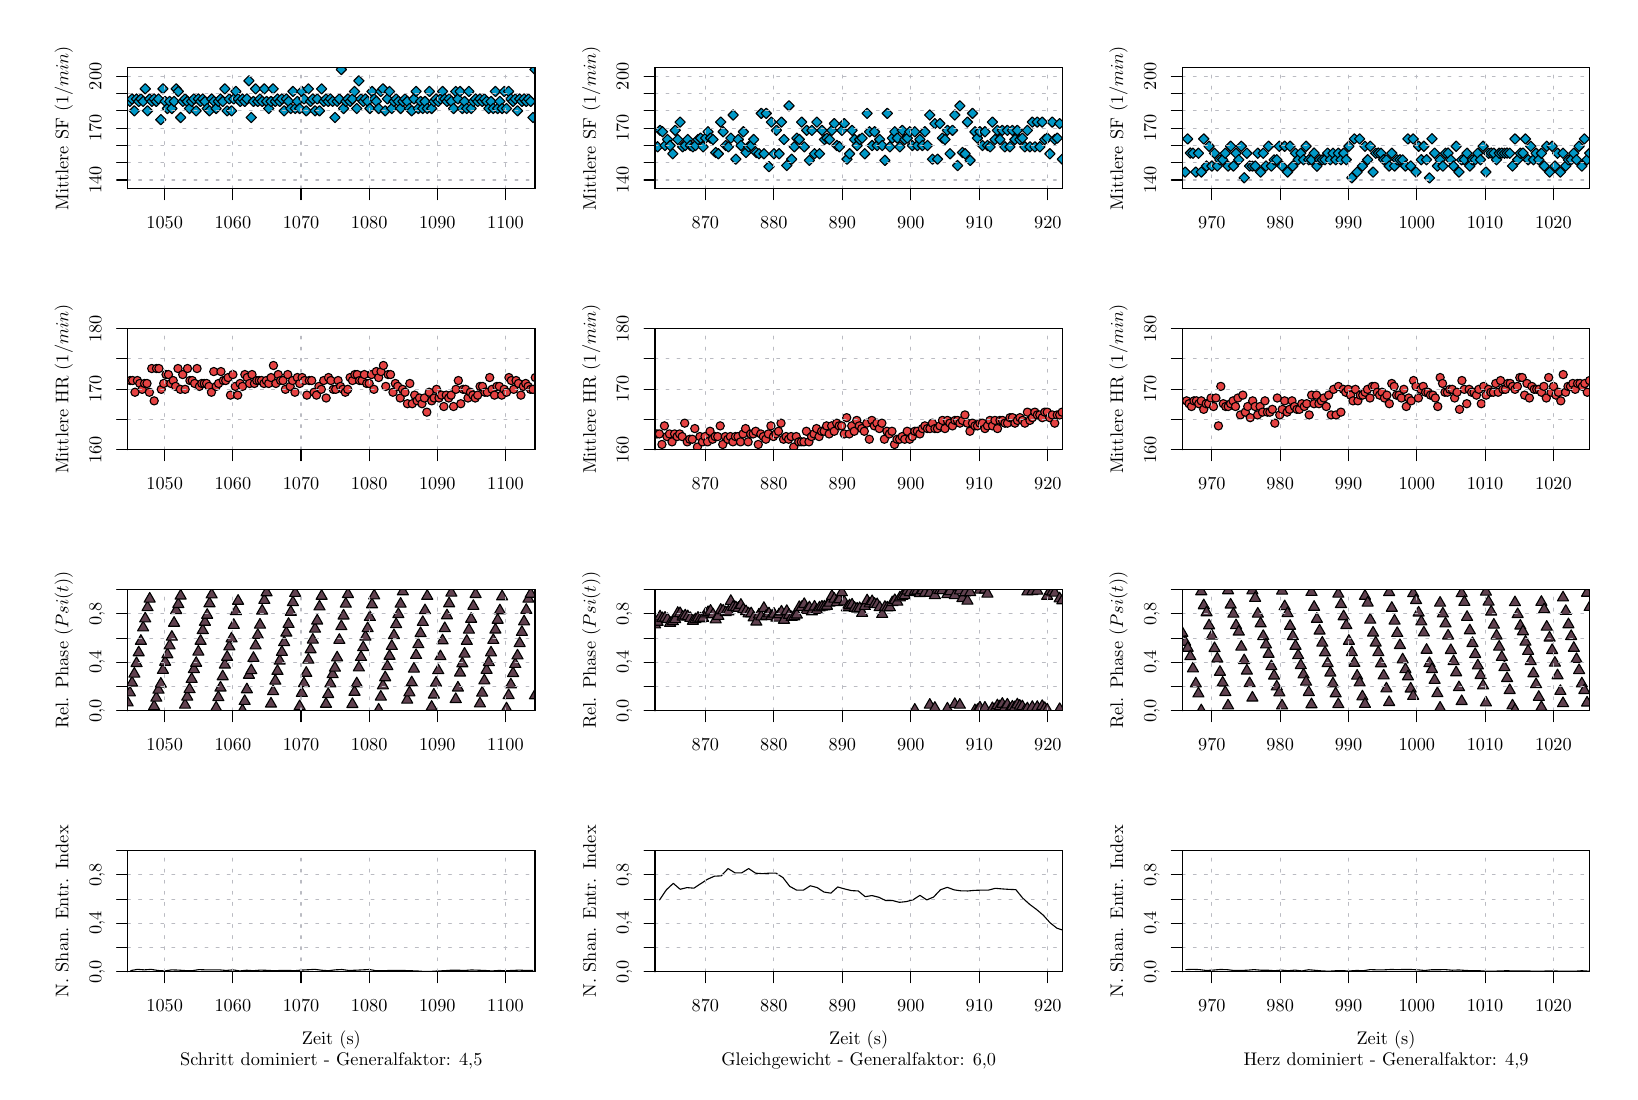
\begin{tikzpicture}[x=1pt,y=1pt]
\definecolor{fillColor}{RGB}{255,255,255}
\path[use as bounding box,fill=fillColor,fill opacity=0.00] (0,0) rectangle (571.66,377.25);
\begin{scope}
\path[clip] ( 36.13,319.07) rectangle (183.32,362.80);
\definecolor{drawColor}{RGB}{0,0,0}
\definecolor{fillColor}{RGB}{0,152,199}

\path[draw=drawColor,line width= 0.4pt,line join=round,line cap=round,fill=fillColor] ( 36.13,232.92) --
	( 38.00,234.78) --
	( 36.13,236.65) --
	( 34.27,234.78) --
	cycle;

\path[draw=drawColor,line width= 0.4pt,line join=round,line cap=round,fill=fillColor] ( 36.93,348.74) --
	( 38.79,350.60) --
	( 36.93,352.46) --
	( 35.07,350.60) --
	cycle;

\path[draw=drawColor,line width= 0.4pt,line join=round,line cap=round,fill=fillColor] ( 37.72,349.63) --
	( 39.58,351.49) --
	( 37.72,353.35) --
	( 35.86,351.49) --
	cycle;

\path[draw=drawColor,line width= 0.4pt,line join=round,line cap=round,fill=fillColor] ( 38.54,345.34) --
	( 40.40,347.20) --
	( 38.54,349.06) --
	( 36.68,347.20) --
	cycle;

\path[draw=drawColor,line width= 0.4pt,line join=round,line cap=round,fill=fillColor] ( 39.33,349.63) --
	( 41.19,351.49) --
	( 39.33,353.35) --
	( 37.47,351.49) --
	cycle;

\path[draw=drawColor,line width= 0.4pt,line join=round,line cap=round,fill=fillColor] ( 40.13,348.74) --
	( 41.99,350.60) --
	( 40.13,352.46) --
	( 38.27,350.60) --
	cycle;

\path[draw=drawColor,line width= 0.4pt,line join=round,line cap=round,fill=fillColor] ( 40.92,349.63) --
	( 42.78,351.49) --
	( 40.92,353.35) --
	( 39.06,351.49) --
	cycle;

\path[draw=drawColor,line width= 0.4pt,line join=round,line cap=round,fill=fillColor] ( 41.72,348.74) --
	( 43.58,350.60) --
	( 41.72,352.46) --
	( 39.86,350.60) --
	cycle;

\path[draw=drawColor,line width= 0.4pt,line join=round,line cap=round,fill=fillColor] ( 42.48,353.29) --
	( 44.35,355.15) --
	( 42.48,357.01) --
	( 40.62,355.15) --
	cycle;

\path[draw=drawColor,line width= 0.4pt,line join=round,line cap=round,fill=fillColor] ( 43.30,345.34) --
	( 45.17,347.20) --
	( 43.30,349.06) --
	( 41.44,347.20) --
	cycle;

\path[draw=drawColor,line width= 0.4pt,line join=round,line cap=round,fill=fillColor] ( 44.10,349.63) --
	( 45.96,351.49) --
	( 44.10,353.35) --
	( 42.23,351.49) --
	cycle;

\path[draw=drawColor,line width= 0.4pt,line join=round,line cap=round,fill=fillColor] ( 44.89,348.74) --
	( 46.75,350.60) --
	( 44.89,352.46) --
	( 43.03,350.60) --
	cycle;

\path[draw=drawColor,line width= 0.4pt,line join=round,line cap=round,fill=fillColor] ( 45.68,349.63) --
	( 47.54,351.49) --
	( 45.68,353.35) --
	( 43.82,351.49) --
	cycle;

\path[draw=drawColor,line width= 0.4pt,line join=round,line cap=round,fill=fillColor] ( 46.48,348.74) --
	( 48.34,350.60) --
	( 46.48,352.46) --
	( 44.62,350.60) --
	cycle;

\path[draw=drawColor,line width= 0.4pt,line join=round,line cap=round,fill=fillColor] ( 47.27,349.63) --
	( 49.13,351.49) --
	( 47.27,353.35) --
	( 45.41,351.49) --
	cycle;

\path[draw=drawColor,line width= 0.4pt,line join=round,line cap=round,fill=fillColor] ( 48.12,342.14) --
	( 49.98,344.00) --
	( 48.12,345.86) --
	( 46.25,344.00) --
	cycle;

\path[draw=drawColor,line width= 0.4pt,line join=round,line cap=round,fill=fillColor] ( 48.88,353.29) --
	( 50.74,355.15) --
	( 48.88,357.01) --
	( 47.02,355.15) --
	cycle;

\path[draw=drawColor,line width= 0.4pt,line join=round,line cap=round,fill=fillColor] ( 49.68,348.74) --
	( 51.54,350.60) --
	( 49.68,352.46) --
	( 47.82,350.60) --
	cycle;

\path[draw=drawColor,line width= 0.4pt,line join=round,line cap=round,fill=fillColor] ( 50.49,346.18) --
	( 52.35,348.04) --
	( 50.49,349.90) --
	( 48.63,348.04) --
	cycle;

\path[draw=drawColor,line width= 0.4pt,line join=round,line cap=round,fill=fillColor] ( 51.29,348.74) --
	( 53.15,350.60) --
	( 51.29,352.46) --
	( 49.43,350.60) --
	cycle;

\path[draw=drawColor,line width= 0.4pt,line join=round,line cap=round,fill=fillColor] ( 52.10,346.18) --
	( 53.97,348.04) --
	( 52.10,349.90) --
	( 50.24,348.04) --
	cycle;

\path[draw=drawColor,line width= 0.4pt,line join=round,line cap=round,fill=fillColor] ( 52.90,348.74) --
	( 54.76,350.60) --
	( 52.90,352.46) --
	( 51.04,350.60) --
	cycle;

\path[draw=drawColor,line width= 0.4pt,line join=round,line cap=round,fill=fillColor] ( 53.67,353.29) --
	( 55.53,355.15) --
	( 53.67,357.01) --
	( 51.81,355.15) --
	cycle;

\path[draw=drawColor,line width= 0.4pt,line join=round,line cap=round,fill=fillColor] ( 54.44,352.34) --
	( 56.30,354.20) --
	( 54.44,356.06) --
	( 52.58,354.20) --
	cycle;

\path[draw=drawColor,line width= 0.4pt,line join=round,line cap=round,fill=fillColor] ( 55.28,342.93) --
	( 57.14,344.79) --
	( 55.28,346.65) --
	( 53.42,344.79) --
	cycle;

\path[draw=drawColor,line width= 0.4pt,line join=round,line cap=round,fill=fillColor] ( 56.08,348.74) --
	( 57.94,350.60) --
	( 56.08,352.46) --
	( 54.21,350.60) --
	cycle;

\path[draw=drawColor,line width= 0.4pt,line join=round,line cap=round,fill=fillColor] ( 56.87,349.63) --
	( 58.73,351.49) --
	( 56.87,353.35) --
	( 55.01,351.49) --
	cycle;

\path[draw=drawColor,line width= 0.4pt,line join=round,line cap=round,fill=fillColor] ( 57.66,348.74) --
	( 59.52,350.60) --
	( 57.66,352.46) --
	( 55.80,350.60) --
	cycle;

\path[draw=drawColor,line width= 0.4pt,line join=round,line cap=round,fill=fillColor] ( 58.48,346.18) --
	( 60.34,348.04) --
	( 58.48,349.90) --
	( 56.62,348.04) --
	cycle;

\path[draw=drawColor,line width= 0.4pt,line join=round,line cap=round,fill=fillColor] ( 59.27,348.74) --
	( 61.14,350.60) --
	( 59.27,352.46) --
	( 57.41,350.60) --
	cycle;

\path[draw=drawColor,line width= 0.4pt,line join=round,line cap=round,fill=fillColor] ( 60.06,349.63) --
	( 61.93,351.49) --
	( 60.06,353.35) --
	( 58.20,351.49) --
	cycle;

\path[draw=drawColor,line width= 0.4pt,line join=round,line cap=round,fill=fillColor] ( 60.89,345.34) --
	( 62.75,347.20) --
	( 60.89,349.06) --
	( 59.02,347.20) --
	cycle;

\path[draw=drawColor,line width= 0.4pt,line join=round,line cap=round,fill=fillColor] ( 61.68,349.63) --
	( 63.54,351.49) --
	( 61.68,353.35) --
	( 59.82,351.49) --
	cycle;

\path[draw=drawColor,line width= 0.4pt,line join=round,line cap=round,fill=fillColor] ( 62.47,348.74) --
	( 64.33,350.60) --
	( 62.47,352.46) --
	( 60.61,350.60) --
	cycle;

\path[draw=drawColor,line width= 0.4pt,line join=round,line cap=round,fill=fillColor] ( 63.26,349.63) --
	( 65.12,351.49) --
	( 63.26,353.35) --
	( 61.40,351.49) --
	cycle;

\path[draw=drawColor,line width= 0.4pt,line join=round,line cap=round,fill=fillColor] ( 64.06,348.74) --
	( 65.92,350.60) --
	( 64.06,352.46) --
	( 62.20,350.60) --
	cycle;

\path[draw=drawColor,line width= 0.4pt,line join=round,line cap=round,fill=fillColor] ( 64.87,346.18) --
	( 66.74,348.04) --
	( 64.87,349.90) --
	( 63.01,348.04) --
	cycle;

\path[draw=drawColor,line width= 0.4pt,line join=round,line cap=round,fill=fillColor] ( 65.70,345.34) --
	( 67.56,347.20) --
	( 65.70,349.06) --
	( 63.83,347.20) --
	cycle;

\path[draw=drawColor,line width= 0.4pt,line join=round,line cap=round,fill=fillColor] ( 66.49,349.63) --
	( 68.35,351.49) --
	( 66.49,353.35) --
	( 64.63,351.49) --
	cycle;

\path[draw=drawColor,line width= 0.4pt,line join=round,line cap=round,fill=fillColor] ( 67.28,348.74) --
	( 69.14,350.60) --
	( 67.28,352.46) --
	( 65.42,350.60) --
	cycle;

\path[draw=drawColor,line width= 0.4pt,line join=round,line cap=round,fill=fillColor] ( 68.10,346.18) --
	( 69.96,348.04) --
	( 68.10,349.90) --
	( 66.24,348.04) --
	cycle;

\path[draw=drawColor,line width= 0.4pt,line join=round,line cap=round,fill=fillColor] ( 68.89,348.74) --
	( 70.76,350.60) --
	( 68.89,352.46) --
	( 67.03,350.60) --
	cycle;

\path[draw=drawColor,line width= 0.4pt,line join=round,line cap=round,fill=fillColor] ( 69.68,349.63) --
	( 71.55,351.49) --
	( 69.68,353.35) --
	( 67.82,351.49) --
	cycle;

\path[draw=drawColor,line width= 0.4pt,line join=round,line cap=round,fill=fillColor] ( 70.48,348.74) --
	( 72.34,350.60) --
	( 70.48,352.46) --
	( 68.62,350.60) --
	cycle;

\path[draw=drawColor,line width= 0.4pt,line join=round,line cap=round,fill=fillColor] ( 71.25,353.29) --
	( 73.11,355.15) --
	( 71.25,357.01) --
	( 69.39,355.15) --
	cycle;

\path[draw=drawColor,line width= 0.4pt,line join=round,line cap=round,fill=fillColor] ( 72.07,345.34) --
	( 73.93,347.20) --
	( 72.07,349.06) --
	( 70.21,347.20) --
	cycle;

\path[draw=drawColor,line width= 0.4pt,line join=round,line cap=round,fill=fillColor] ( 72.86,349.63) --
	( 74.72,351.49) --
	( 72.86,353.35) --
	( 71.00,351.49) --
	cycle;

\path[draw=drawColor,line width= 0.4pt,line join=round,line cap=round,fill=fillColor] ( 73.68,345.34) --
	( 75.54,347.20) --
	( 73.68,349.06) --
	( 71.82,347.20) --
	cycle;

\path[draw=drawColor,line width= 0.4pt,line join=round,line cap=round,fill=fillColor] ( 74.47,349.63) --
	( 76.33,351.49) --
	( 74.47,353.35) --
	( 72.61,351.49) --
	cycle;

\path[draw=drawColor,line width= 0.4pt,line join=round,line cap=round,fill=fillColor] ( 75.24,352.34) --
	( 77.10,354.20) --
	( 75.24,356.06) --
	( 73.38,354.20) --
	cycle;

\path[draw=drawColor,line width= 0.4pt,line join=round,line cap=round,fill=fillColor] ( 76.03,349.63) --
	( 77.90,351.49) --
	( 76.03,353.35) --
	( 74.17,351.49) --
	cycle;

\path[draw=drawColor,line width= 0.4pt,line join=round,line cap=round,fill=fillColor] ( 76.83,348.74) --
	( 78.69,350.60) --
	( 76.83,352.46) --
	( 74.97,350.60) --
	cycle;

\path[draw=drawColor,line width= 0.4pt,line join=round,line cap=round,fill=fillColor] ( 77.62,349.63) --
	( 79.48,351.49) --
	( 77.62,353.35) --
	( 75.76,351.49) --
	cycle;

\path[draw=drawColor,line width= 0.4pt,line join=round,line cap=round,fill=fillColor] ( 78.42,348.74) --
	( 80.28,350.60) --
	( 78.42,352.46) --
	( 76.56,350.60) --
	cycle;

\path[draw=drawColor,line width= 0.4pt,line join=round,line cap=round,fill=fillColor] ( 79.21,349.63) --
	( 81.07,351.49) --
	( 79.21,353.35) --
	( 77.35,351.49) --
	cycle;

\path[draw=drawColor,line width= 0.4pt,line join=round,line cap=round,fill=fillColor] ( 79.96,356.18) --
	( 81.82,358.04) --
	( 79.96,359.90) --
	( 78.10,358.04) --
	cycle;

\path[draw=drawColor,line width= 0.4pt,line join=round,line cap=round,fill=fillColor] ( 80.80,342.93) --
	( 82.66,344.79) --
	( 80.80,346.65) --
	( 78.93,344.79) --
	cycle;

\path[draw=drawColor,line width= 0.4pt,line join=round,line cap=round,fill=fillColor] ( 81.59,348.74) --
	( 83.45,350.60) --
	( 81.59,352.46) --
	( 79.73,350.60) --
	cycle;

\path[draw=drawColor,line width= 0.4pt,line join=round,line cap=round,fill=fillColor] ( 82.36,353.29) --
	( 84.22,355.15) --
	( 82.36,357.01) --
	( 80.50,355.15) --
	cycle;

\path[draw=drawColor,line width= 0.4pt,line join=round,line cap=round,fill=fillColor] ( 83.16,348.74) --
	( 85.02,350.60) --
	( 83.16,352.46) --
	( 81.29,350.60) --
	cycle;

\path[draw=drawColor,line width= 0.4pt,line join=round,line cap=round,fill=fillColor] ( 83.95,349.63) --
	( 85.81,351.49) --
	( 83.95,353.35) --
	( 82.09,351.49) --
	cycle;

\path[draw=drawColor,line width= 0.4pt,line join=round,line cap=round,fill=fillColor] ( 84.74,348.74) --
	( 86.60,350.60) --
	( 84.74,352.46) --
	( 82.88,350.60) --
	cycle;

\path[draw=drawColor,line width= 0.4pt,line join=round,line cap=round,fill=fillColor] ( 85.51,353.29) --
	( 87.37,355.15) --
	( 85.51,357.01) --
	( 83.65,355.15) --
	cycle;

\path[draw=drawColor,line width= 0.4pt,line join=round,line cap=round,fill=fillColor] ( 86.31,348.74) --
	( 88.17,350.60) --
	( 86.31,352.46) --
	( 84.45,350.60) --
	cycle;

\path[draw=drawColor,line width= 0.4pt,line join=round,line cap=round,fill=fillColor] ( 87.12,346.18) --
	( 88.98,348.04) --
	( 87.12,349.90) --
	( 85.26,348.04) --
	cycle;

\path[draw=drawColor,line width= 0.4pt,line join=round,line cap=round,fill=fillColor] ( 87.92,348.74) --
	( 89.78,350.60) --
	( 87.92,352.46) --
	( 86.06,350.60) --
	cycle;

\path[draw=drawColor,line width= 0.4pt,line join=round,line cap=round,fill=fillColor] ( 88.68,353.29) --
	( 90.55,355.15) --
	( 88.68,357.01) --
	( 86.82,355.15) --
	cycle;

\path[draw=drawColor,line width= 0.4pt,line join=round,line cap=round,fill=fillColor] ( 89.48,348.74) --
	( 91.34,350.60) --
	( 89.48,352.46) --
	( 87.62,350.60) --
	cycle;

\path[draw=drawColor,line width= 0.4pt,line join=round,line cap=round,fill=fillColor] ( 90.27,349.63) --
	( 92.13,351.49) --
	( 90.27,353.35) --
	( 88.41,351.49) --
	cycle;

\path[draw=drawColor,line width= 0.4pt,line join=round,line cap=round,fill=fillColor] ( 91.07,348.74) --
	( 92.93,350.60) --
	( 91.07,352.46) --
	( 89.21,350.60) --
	cycle;

\path[draw=drawColor,line width= 0.4pt,line join=round,line cap=round,fill=fillColor] ( 91.86,349.63) --
	( 93.72,351.49) --
	( 91.86,353.35) --
	( 90.00,351.49) --
	cycle;

\path[draw=drawColor,line width= 0.4pt,line join=round,line cap=round,fill=fillColor] ( 92.68,345.34) --
	( 94.54,347.20) --
	( 92.68,349.06) --
	( 90.82,347.20) --
	cycle;

\path[draw=drawColor,line width= 0.4pt,line join=round,line cap=round,fill=fillColor] ( 93.47,349.63) --
	( 95.33,351.49) --
	( 93.47,353.35) --
	( 91.61,351.49) --
	cycle;

\path[draw=drawColor,line width= 0.4pt,line join=round,line cap=round,fill=fillColor] ( 94.27,348.74) --
	( 96.13,350.60) --
	( 94.27,352.46) --
	( 92.41,350.60) --
	cycle;

\path[draw=drawColor,line width= 0.4pt,line join=round,line cap=round,fill=fillColor] ( 95.08,346.18) --
	( 96.94,348.04) --
	( 95.08,349.90) --
	( 93.22,348.04) --
	cycle;

\path[draw=drawColor,line width= 0.4pt,line join=round,line cap=round,fill=fillColor] ( 95.85,352.34) --
	( 97.72,354.20) --
	( 95.85,356.06) --
	( 93.99,354.20) --
	cycle;

\path[draw=drawColor,line width= 0.4pt,line join=round,line cap=round,fill=fillColor] ( 96.67,346.18) --
	( 98.53,348.04) --
	( 96.67,349.90) --
	( 94.81,348.04) --
	cycle;

\path[draw=drawColor,line width= 0.4pt,line join=round,line cap=round,fill=fillColor] ( 97.47,348.74) --
	( 99.33,350.60) --
	( 97.47,352.46) --
	( 95.60,350.60) --
	cycle;

\path[draw=drawColor,line width= 0.4pt,line join=round,line cap=round,fill=fillColor] ( 98.28,346.18) --
	(100.14,348.04) --
	( 98.28,349.90) --
	( 96.42,348.04) --
	cycle;

\path[draw=drawColor,line width= 0.4pt,line join=round,line cap=round,fill=fillColor] ( 99.05,352.34) --
	(100.91,354.20) --
	( 99.05,356.06) --
	( 97.19,354.20) --
	cycle;

\path[draw=drawColor,line width= 0.4pt,line join=round,line cap=round,fill=fillColor] ( 99.84,349.63) --
	(101.70,351.49) --
	( 99.84,353.35) --
	( 97.98,351.49) --
	cycle;

\path[draw=drawColor,line width= 0.4pt,line join=round,line cap=round,fill=fillColor] (100.66,345.34) --
	(102.53,347.20) --
	(100.66,349.06) --
	( 98.80,347.20) --
	cycle;

\path[draw=drawColor,line width= 0.4pt,line join=round,line cap=round,fill=fillColor] (101.43,353.29) --
	(103.29,355.15) --
	(101.43,357.01) --
	( 99.57,355.15) --
	cycle;

\path[draw=drawColor,line width= 0.4pt,line join=round,line cap=round,fill=fillColor] (102.23,348.74) --
	(104.09,350.60) --
	(102.23,352.46) --
	(100.37,350.60) --
	cycle;

\path[draw=drawColor,line width= 0.4pt,line join=round,line cap=round,fill=fillColor] (103.02,349.63) --
	(104.88,351.49) --
	(103.02,353.35) --
	(101.16,351.49) --
	cycle;

\path[draw=drawColor,line width= 0.4pt,line join=round,line cap=round,fill=fillColor] (103.84,345.34) --
	(105.70,347.20) --
	(103.84,349.06) --
	(101.98,347.20) --
	cycle;

\path[draw=drawColor,line width= 0.4pt,line join=round,line cap=round,fill=fillColor] (104.63,349.63) --
	(106.49,351.49) --
	(104.63,353.35) --
	(102.77,351.49) --
	cycle;

\path[draw=drawColor,line width= 0.4pt,line join=round,line cap=round,fill=fillColor] (105.45,345.34) --
	(107.31,347.20) --
	(105.45,349.06) --
	(103.59,347.20) --
	cycle;

\path[draw=drawColor,line width= 0.4pt,line join=round,line cap=round,fill=fillColor] (106.22,353.29) --
	(108.08,355.15) --
	(106.22,357.01) --
	(104.36,355.15) --
	cycle;

\path[draw=drawColor,line width= 0.4pt,line join=round,line cap=round,fill=fillColor] (107.01,348.74) --
	(108.87,350.60) --
	(107.01,352.46) --
	(105.15,350.60) --
	cycle;

\path[draw=drawColor,line width= 0.4pt,line join=round,line cap=round,fill=fillColor] (107.80,349.63) --
	(109.67,351.49) --
	(107.80,353.35) --
	(105.94,351.49) --
	cycle;

\path[draw=drawColor,line width= 0.4pt,line join=round,line cap=round,fill=fillColor] (108.60,348.74) --
	(110.46,350.60) --
	(108.60,352.46) --
	(106.74,350.60) --
	cycle;

\path[draw=drawColor,line width= 0.4pt,line join=round,line cap=round,fill=fillColor] (109.39,349.63) --
	(111.25,351.49) --
	(109.39,353.35) --
	(107.53,351.49) --
	cycle;

\path[draw=drawColor,line width= 0.4pt,line join=round,line cap=round,fill=fillColor] (110.19,348.74) --
	(112.05,350.60) --
	(110.19,352.46) --
	(108.33,350.60) --
	cycle;

\path[draw=drawColor,line width= 0.4pt,line join=round,line cap=round,fill=fillColor] (111.03,342.93) --
	(112.89,344.79) --
	(111.03,346.65) --
	(109.17,344.79) --
	cycle;

\path[draw=drawColor,line width= 0.4pt,line join=round,line cap=round,fill=fillColor] (111.82,348.74) --
	(113.69,350.60) --
	(111.82,352.46) --
	(109.96,350.60) --
	cycle;

\path[draw=drawColor,line width= 0.4pt,line join=round,line cap=round,fill=fillColor] (112.61,349.63) --
	(114.48,351.49) --
	(112.61,353.35) --
	(110.75,351.49) --
	cycle;

\path[draw=drawColor,line width= 0.4pt,line join=round,line cap=round,fill=fillColor] (113.34,360.27) --
	(115.20,362.13) --
	(113.34,363.99) --
	(111.48,362.13) --
	cycle;

\path[draw=drawColor,line width= 0.4pt,line join=round,line cap=round,fill=fillColor] (114.15,346.18) --
	(116.01,348.04) --
	(114.15,349.90) --
	(112.29,348.04) --
	cycle;

\path[draw=drawColor,line width= 0.4pt,line join=round,line cap=round,fill=fillColor] (114.95,348.74) --
	(116.81,350.60) --
	(114.95,352.46) --
	(113.09,350.60) --
	cycle;

\path[draw=drawColor,line width= 0.4pt,line join=round,line cap=round,fill=fillColor] (115.74,349.63) --
	(117.60,351.49) --
	(115.74,353.35) --
	(113.88,351.49) --
	cycle;

\path[draw=drawColor,line width= 0.4pt,line join=round,line cap=round,fill=fillColor] (116.54,348.74) --
	(118.40,350.60) --
	(116.54,352.46) --
	(114.68,350.60) --
	cycle;

\path[draw=drawColor,line width= 0.4pt,line join=round,line cap=round,fill=fillColor] (117.33,349.63) --
	(119.19,351.49) --
	(117.33,353.35) --
	(115.47,351.49) --
	cycle;

\path[draw=drawColor,line width= 0.4pt,line join=round,line cap=round,fill=fillColor] (118.10,352.34) --
	(119.96,354.20) --
	(118.10,356.06) --
	(116.24,354.20) --
	cycle;

\path[draw=drawColor,line width= 0.4pt,line join=round,line cap=round,fill=fillColor] (118.92,346.18) --
	(120.78,348.04) --
	(118.92,349.90) --
	(117.05,348.04) --
	cycle;

\path[draw=drawColor,line width= 0.4pt,line join=round,line cap=round,fill=fillColor] (119.66,356.18) --
	(121.53,358.04) --
	(119.66,359.90) --
	(117.80,358.04) --
	cycle;

\path[draw=drawColor,line width= 0.4pt,line join=round,line cap=round,fill=fillColor] (120.45,349.63) --
	(122.32,351.49) --
	(120.45,353.35) --
	(118.59,351.49) --
	cycle;

\path[draw=drawColor,line width= 0.4pt,line join=round,line cap=round,fill=fillColor] (121.25,348.74) --
	(123.11,350.60) --
	(121.25,352.46) --
	(119.39,350.60) --
	cycle;

\path[draw=drawColor,line width= 0.4pt,line join=round,line cap=round,fill=fillColor] (122.04,349.63) --
	(123.90,351.49) --
	(122.04,353.35) --
	(120.18,351.49) --
	cycle;

\path[draw=drawColor,line width= 0.4pt,line join=round,line cap=round,fill=fillColor] (122.84,348.74) --
	(124.70,350.60) --
	(122.84,352.46) --
	(120.98,350.60) --
	cycle;

\path[draw=drawColor,line width= 0.4pt,line join=round,line cap=round,fill=fillColor] (123.65,346.18) --
	(125.51,348.04) --
	(123.65,349.90) --
	(121.79,348.04) --
	cycle;

\path[draw=drawColor,line width= 0.4pt,line join=round,line cap=round,fill=fillColor] (124.43,352.34) --
	(126.29,354.20) --
	(124.43,356.06) --
	(122.56,354.20) --
	cycle;

\path[draw=drawColor,line width= 0.4pt,line join=round,line cap=round,fill=fillColor] (125.22,349.63) --
	(127.08,351.49) --
	(125.22,353.35) --
	(123.36,351.49) --
	cycle;

\path[draw=drawColor,line width= 0.4pt,line join=round,line cap=round,fill=fillColor] (126.01,348.74) --
	(127.87,350.60) --
	(126.01,352.46) --
	(124.15,350.60) --
	cycle;

\path[draw=drawColor,line width= 0.4pt,line join=round,line cap=round,fill=fillColor] (126.83,346.18) --
	(128.69,348.04) --
	(126.83,349.90) --
	(124.97,348.04) --
	cycle;

\path[draw=drawColor,line width= 0.4pt,line join=round,line cap=round,fill=fillColor] (127.60,352.34) --
	(129.46,354.20) --
	(127.60,356.06) --
	(125.74,354.20) --
	cycle;

\path[draw=drawColor,line width= 0.4pt,line join=round,line cap=round,fill=fillColor] (128.37,353.29) --
	(130.23,355.15) --
	(128.37,357.01) --
	(126.51,355.15) --
	cycle;

\path[draw=drawColor,line width= 0.4pt,line join=round,line cap=round,fill=fillColor] (129.19,345.34) --
	(131.05,347.20) --
	(129.19,349.06) --
	(127.33,347.20) --
	cycle;

\path[draw=drawColor,line width= 0.4pt,line join=round,line cap=round,fill=fillColor] (129.98,349.63) --
	(131.84,351.49) --
	(129.98,353.35) --
	(128.12,351.49) --
	cycle;

\path[draw=drawColor,line width= 0.4pt,line join=round,line cap=round,fill=fillColor] (130.75,352.34) --
	(132.61,354.20) --
	(130.75,356.06) --
	(128.89,354.20) --
	cycle;

\path[draw=drawColor,line width= 0.4pt,line join=round,line cap=round,fill=fillColor] (131.57,346.18) --
	(133.43,348.04) --
	(131.57,349.90) --
	(129.70,348.04) --
	cycle;

\path[draw=drawColor,line width= 0.4pt,line join=round,line cap=round,fill=fillColor] (132.36,348.74) --
	(134.22,350.60) --
	(132.36,352.46) --
	(130.50,350.60) --
	cycle;

\path[draw=drawColor,line width= 0.4pt,line join=round,line cap=round,fill=fillColor] (133.15,349.63) --
	(135.01,351.49) --
	(133.15,353.35) --
	(131.29,351.49) --
	cycle;

\path[draw=drawColor,line width= 0.4pt,line join=round,line cap=round,fill=fillColor] (133.95,348.74) --
	(135.81,350.60) --
	(133.95,352.46) --
	(132.09,350.60) --
	cycle;

\path[draw=drawColor,line width= 0.4pt,line join=round,line cap=round,fill=fillColor] (134.76,346.18) --
	(136.63,348.04) --
	(134.76,349.90) --
	(132.90,348.04) --
	cycle;

\path[draw=drawColor,line width= 0.4pt,line join=round,line cap=round,fill=fillColor] (135.56,348.74) --
	(137.42,350.60) --
	(135.56,352.46) --
	(133.70,350.60) --
	cycle;

\path[draw=drawColor,line width= 0.4pt,line join=round,line cap=round,fill=fillColor] (136.35,349.63) --
	(138.21,351.49) --
	(136.35,353.35) --
	(134.49,351.49) --
	cycle;

\path[draw=drawColor,line width= 0.4pt,line join=round,line cap=round,fill=fillColor] (137.15,348.74) --
	(139.01,350.60) --
	(137.15,352.46) --
	(135.29,350.60) --
	cycle;

\path[draw=drawColor,line width= 0.4pt,line join=round,line cap=round,fill=fillColor] (137.96,346.18) --
	(139.82,348.04) --
	(137.96,349.90) --
	(136.10,348.04) --
	cycle;

\path[draw=drawColor,line width= 0.4pt,line join=round,line cap=round,fill=fillColor] (138.78,345.34) --
	(140.65,347.20) --
	(138.78,349.06) --
	(136.92,347.20) --
	cycle;

\path[draw=drawColor,line width= 0.4pt,line join=round,line cap=round,fill=fillColor] (139.57,349.63) --
	(141.44,351.49) --
	(139.57,353.35) --
	(137.71,351.49) --
	cycle;

\path[draw=drawColor,line width= 0.4pt,line join=round,line cap=round,fill=fillColor] (140.35,352.34) --
	(142.21,354.20) --
	(140.35,356.06) --
	(138.49,354.20) --
	cycle;

\path[draw=drawColor,line width= 0.4pt,line join=round,line cap=round,fill=fillColor] (141.16,346.18) --
	(143.02,348.04) --
	(141.16,349.90) --
	(139.30,348.04) --
	cycle;

\path[draw=drawColor,line width= 0.4pt,line join=round,line cap=round,fill=fillColor] (141.96,348.74) --
	(143.82,350.60) --
	(141.96,352.46) --
	(140.10,350.60) --
	cycle;

\path[draw=drawColor,line width= 0.4pt,line join=round,line cap=round,fill=fillColor] (142.77,346.18) --
	(144.63,348.04) --
	(142.77,349.90) --
	(140.91,348.04) --
	cycle;

\path[draw=drawColor,line width= 0.4pt,line join=round,line cap=round,fill=fillColor] (143.57,348.74) --
	(145.43,350.60) --
	(143.57,352.46) --
	(141.71,350.60) --
	cycle;

\path[draw=drawColor,line width= 0.4pt,line join=round,line cap=round,fill=fillColor] (144.38,346.18) --
	(146.25,348.04) --
	(144.38,349.90) --
	(142.52,348.04) --
	cycle;

\path[draw=drawColor,line width= 0.4pt,line join=round,line cap=round,fill=fillColor] (145.16,352.34) --
	(147.02,354.20) --
	(145.16,356.06) --
	(143.30,354.20) --
	cycle;

\path[draw=drawColor,line width= 0.4pt,line join=round,line cap=round,fill=fillColor] (145.97,346.18) --
	(147.83,348.04) --
	(145.97,349.90) --
	(144.11,348.04) --
	cycle;

\path[draw=drawColor,line width= 0.4pt,line join=round,line cap=round,fill=fillColor] (146.77,348.74) --
	(148.63,350.60) --
	(146.77,352.46) --
	(144.91,350.60) --
	cycle;

\path[draw=drawColor,line width= 0.4pt,line join=round,line cap=round,fill=fillColor] (147.56,349.63) --
	(149.42,351.49) --
	(147.56,353.35) --
	(145.70,351.49) --
	cycle;

\path[draw=drawColor,line width= 0.4pt,line join=round,line cap=round,fill=fillColor] (148.36,348.74) --
	(150.22,350.60) --
	(148.36,352.46) --
	(146.49,350.60) --
	cycle;

\path[draw=drawColor,line width= 0.4pt,line join=round,line cap=round,fill=fillColor] (149.15,349.63) --
	(151.01,351.49) --
	(149.15,353.35) --
	(147.29,351.49) --
	cycle;

\path[draw=drawColor,line width= 0.4pt,line join=round,line cap=round,fill=fillColor] (149.92,352.34) --
	(151.78,354.20) --
	(149.92,356.06) --
	(148.06,354.20) --
	cycle;

\path[draw=drawColor,line width= 0.4pt,line join=round,line cap=round,fill=fillColor] (150.71,349.63) --
	(152.57,351.49) --
	(150.71,353.35) --
	(148.85,351.49) --
	cycle;

\path[draw=drawColor,line width= 0.4pt,line join=round,line cap=round,fill=fillColor] (151.51,348.74) --
	(153.37,350.60) --
	(151.51,352.46) --
	(149.65,350.60) --
	cycle;

\path[draw=drawColor,line width= 0.4pt,line join=round,line cap=round,fill=fillColor] (152.30,349.63) --
	(154.16,351.49) --
	(152.30,353.35) --
	(150.44,351.49) --
	cycle;

\path[draw=drawColor,line width= 0.4pt,line join=round,line cap=round,fill=fillColor] (153.09,348.74) --
	(154.96,350.60) --
	(153.09,352.46) --
	(151.23,350.60) --
	cycle;

\path[draw=drawColor,line width= 0.4pt,line join=round,line cap=round,fill=fillColor] (153.91,346.18) --
	(155.77,348.04) --
	(153.91,349.90) --
	(152.05,348.04) --
	cycle;

\path[draw=drawColor,line width= 0.4pt,line join=round,line cap=round,fill=fillColor] (154.68,352.34) --
	(156.54,354.20) --
	(154.68,356.06) --
	(152.82,354.20) --
	cycle;

\path[draw=drawColor,line width= 0.4pt,line join=round,line cap=round,fill=fillColor] (155.47,349.63) --
	(157.33,351.49) --
	(155.47,353.35) --
	(153.61,351.49) --
	cycle;

\path[draw=drawColor,line width= 0.4pt,line join=round,line cap=round,fill=fillColor] (156.24,352.34) --
	(158.11,354.20) --
	(156.24,356.06) --
	(154.38,354.20) --
	cycle;

\path[draw=drawColor,line width= 0.4pt,line join=round,line cap=round,fill=fillColor] (157.06,346.18) --
	(158.92,348.04) --
	(157.06,349.90) --
	(155.20,348.04) --
	cycle;

\path[draw=drawColor,line width= 0.4pt,line join=round,line cap=round,fill=fillColor] (157.86,348.74) --
	(159.72,350.60) --
	(157.86,352.46) --
	(155.99,350.60) --
	cycle;

\path[draw=drawColor,line width= 0.4pt,line join=round,line cap=round,fill=fillColor] (158.67,346.18) --
	(160.53,348.04) --
	(158.67,349.90) --
	(156.81,348.04) --
	cycle;

\path[draw=drawColor,line width= 0.4pt,line join=round,line cap=round,fill=fillColor] (159.44,352.34) --
	(161.30,354.20) --
	(159.44,356.06) --
	(157.58,354.20) --
	cycle;

\path[draw=drawColor,line width= 0.4pt,line join=round,line cap=round,fill=fillColor] (160.26,346.18) --
	(162.12,348.04) --
	(160.26,349.90) --
	(158.40,348.04) --
	cycle;

\path[draw=drawColor,line width= 0.4pt,line join=round,line cap=round,fill=fillColor] (161.05,348.74) --
	(162.92,350.60) --
	(161.05,352.46) --
	(159.19,350.60) --
	cycle;

\path[draw=drawColor,line width= 0.4pt,line join=round,line cap=round,fill=fillColor] (161.85,349.63) --
	(163.71,351.49) --
	(161.85,353.35) --
	(159.98,351.49) --
	cycle;

\path[draw=drawColor,line width= 0.4pt,line join=round,line cap=round,fill=fillColor] (162.64,348.74) --
	(164.50,350.60) --
	(162.64,352.46) --
	(160.78,350.60) --
	cycle;

\path[draw=drawColor,line width= 0.4pt,line join=round,line cap=round,fill=fillColor] (163.43,349.63) --
	(165.29,351.49) --
	(163.43,353.35) --
	(161.57,351.49) --
	cycle;

\path[draw=drawColor,line width= 0.4pt,line join=round,line cap=round,fill=fillColor] (164.23,348.74) --
	(166.09,350.60) --
	(164.23,352.46) --
	(162.37,350.60) --
	cycle;

\path[draw=drawColor,line width= 0.4pt,line join=round,line cap=round,fill=fillColor] (165.02,349.63) --
	(166.88,351.49) --
	(165.02,353.35) --
	(163.16,351.49) --
	cycle;

\path[draw=drawColor,line width= 0.4pt,line join=round,line cap=round,fill=fillColor] (165.82,348.74) --
	(167.68,350.60) --
	(165.82,352.46) --
	(163.96,350.60) --
	cycle;

\path[draw=drawColor,line width= 0.4pt,line join=round,line cap=round,fill=fillColor] (166.63,346.18) --
	(168.49,348.04) --
	(166.63,349.90) --
	(164.77,348.04) --
	cycle;

\path[draw=drawColor,line width= 0.4pt,line join=round,line cap=round,fill=fillColor] (167.43,348.74) --
	(169.29,350.60) --
	(167.43,352.46) --
	(165.57,350.60) --
	cycle;

\path[draw=drawColor,line width= 0.4pt,line join=round,line cap=round,fill=fillColor] (168.24,346.18) --
	(170.10,348.04) --
	(168.24,349.90) --
	(166.38,348.04) --
	cycle;

\path[draw=drawColor,line width= 0.4pt,line join=round,line cap=round,fill=fillColor] (169.02,352.34) --
	(170.88,354.20) --
	(169.02,356.06) --
	(167.15,354.20) --
	cycle;

\path[draw=drawColor,line width= 0.4pt,line join=round,line cap=round,fill=fillColor] (169.83,346.18) --
	(171.69,348.04) --
	(169.83,349.90) --
	(167.97,348.04) --
	cycle;

\path[draw=drawColor,line width= 0.4pt,line join=round,line cap=round,fill=fillColor] (170.63,348.74) --
	(172.49,350.60) --
	(170.63,352.46) --
	(168.77,350.60) --
	cycle;

\path[draw=drawColor,line width= 0.4pt,line join=round,line cap=round,fill=fillColor] (171.44,346.18) --
	(173.30,348.04) --
	(171.44,349.90) --
	(169.58,348.04) --
	cycle;

\path[draw=drawColor,line width= 0.4pt,line join=round,line cap=round,fill=fillColor] (172.21,352.34) --
	(174.07,354.20) --
	(172.21,356.06) --
	(170.35,354.20) --
	cycle;

\path[draw=drawColor,line width= 0.4pt,line join=round,line cap=round,fill=fillColor] (173.03,346.18) --
	(174.89,348.04) --
	(173.03,349.90) --
	(171.17,348.04) --
	cycle;

\path[draw=drawColor,line width= 0.4pt,line join=round,line cap=round,fill=fillColor] (173.80,352.34) --
	(175.66,354.20) --
	(173.80,356.06) --
	(171.94,354.20) --
	cycle;

\path[draw=drawColor,line width= 0.4pt,line join=round,line cap=round,fill=fillColor] (174.59,349.63) --
	(176.45,351.49) --
	(174.59,353.35) --
	(172.73,351.49) --
	cycle;

\path[draw=drawColor,line width= 0.4pt,line join=round,line cap=round,fill=fillColor] (175.39,348.74) --
	(177.25,350.60) --
	(175.39,352.46) --
	(173.53,350.60) --
	cycle;

\path[draw=drawColor,line width= 0.4pt,line join=round,line cap=round,fill=fillColor] (176.18,349.63) --
	(178.04,351.49) --
	(176.18,353.35) --
	(174.32,351.49) --
	cycle;

\path[draw=drawColor,line width= 0.4pt,line join=round,line cap=round,fill=fillColor] (177.00,345.34) --
	(178.86,347.20) --
	(177.00,349.06) --
	(175.14,347.20) --
	cycle;

\path[draw=drawColor,line width= 0.4pt,line join=round,line cap=round,fill=fillColor] (177.79,349.63) --
	(179.65,351.49) --
	(177.79,353.35) --
	(175.93,351.49) --
	cycle;

\path[draw=drawColor,line width= 0.4pt,line join=round,line cap=round,fill=fillColor] (178.59,348.74) --
	(180.45,350.60) --
	(178.59,352.46) --
	(176.73,350.60) --
	cycle;

\path[draw=drawColor,line width= 0.4pt,line join=round,line cap=round,fill=fillColor] (179.38,349.63) --
	(181.24,351.49) --
	(179.38,353.35) --
	(177.52,351.49) --
	cycle;

\path[draw=drawColor,line width= 0.4pt,line join=round,line cap=round,fill=fillColor] (180.17,348.74) --
	(182.04,350.60) --
	(180.17,352.46) --
	(178.31,350.60) --
	cycle;

\path[draw=drawColor,line width= 0.4pt,line join=round,line cap=round,fill=fillColor] (180.96,349.63) --
	(182.83,351.49) --
	(180.96,353.35) --
	(179.10,351.49) --
	cycle;

\path[draw=drawColor,line width= 0.4pt,line join=round,line cap=round,fill=fillColor] (181.76,348.74) --
	(183.62,350.60) --
	(181.76,352.46) --
	(179.90,350.60) --
	cycle;

\path[draw=drawColor,line width= 0.4pt,line join=round,line cap=round,fill=fillColor] (182.60,342.93) --
	(184.46,344.79) --
	(182.60,346.65) --
	(180.74,344.79) --
	cycle;

\path[draw=drawColor,line width= 0.4pt,line join=round,line cap=round,fill=fillColor] (183.32,360.27) --
	(185.19,362.13) --
	(183.32,363.99) --
	(181.46,362.13) --
	cycle;
\end{scope}
\begin{scope}
\path[clip] (  0.00,  0.00) rectangle (571.66,377.25);
\definecolor{drawColor}{RGB}{0,0,0}

\path[draw=drawColor,line width= 0.4pt,line join=round,line cap=round] ( 49.53,319.07) -- (172.66,319.07);

\path[draw=drawColor,line width= 0.4pt,line join=round,line cap=round] ( 49.53,319.07) -- ( 49.53,315.11);

\path[draw=drawColor,line width= 0.4pt,line join=round,line cap=round] ( 74.15,319.07) -- ( 74.15,315.11);

\path[draw=drawColor,line width= 0.4pt,line join=round,line cap=round] ( 98.78,319.07) -- ( 98.78,315.11);

\path[draw=drawColor,line width= 0.4pt,line join=round,line cap=round] (123.41,319.07) -- (123.41,315.11);

\path[draw=drawColor,line width= 0.4pt,line join=round,line cap=round] (148.03,319.07) -- (148.03,315.11);

\path[draw=drawColor,line width= 0.4pt,line join=round,line cap=round] (172.66,319.07) -- (172.66,315.11);

\node[text=drawColor,anchor=base,inner sep=0pt, outer sep=0pt, scale=  0.66] at ( 49.53,304.82) {1050};

\node[text=drawColor,anchor=base,inner sep=0pt, outer sep=0pt, scale=  0.66] at ( 74.15,304.82) {1060};

\node[text=drawColor,anchor=base,inner sep=0pt, outer sep=0pt, scale=  0.66] at ( 98.78,304.82) {1070};

\node[text=drawColor,anchor=base,inner sep=0pt, outer sep=0pt, scale=  0.66] at (123.41,304.82) {1080};

\node[text=drawColor,anchor=base,inner sep=0pt, outer sep=0pt, scale=  0.66] at (148.03,304.82) {1090};

\node[text=drawColor,anchor=base,inner sep=0pt, outer sep=0pt, scale=  0.66] at (172.66,304.82) {1100};

\path[draw=drawColor,line width= 0.4pt,line join=round,line cap=round] ( 36.13,322.20) -- ( 36.13,359.67);

\path[draw=drawColor,line width= 0.4pt,line join=round,line cap=round] ( 36.13,322.20) -- ( 32.17,322.20);

\path[draw=drawColor,line width= 0.4pt,line join=round,line cap=round] ( 36.13,328.44) -- ( 32.17,328.44);

\path[draw=drawColor,line width= 0.4pt,line join=round,line cap=round] ( 36.13,334.69) -- ( 32.17,334.69);

\path[draw=drawColor,line width= 0.4pt,line join=round,line cap=round] ( 36.13,340.93) -- ( 32.17,340.93);

\path[draw=drawColor,line width= 0.4pt,line join=round,line cap=round] ( 36.13,347.18) -- ( 32.17,347.18);

\path[draw=drawColor,line width= 0.4pt,line join=round,line cap=round] ( 36.13,353.43) -- ( 32.17,353.43);

\path[draw=drawColor,line width= 0.4pt,line join=round,line cap=round] ( 36.13,359.67) -- ( 32.17,359.67);

\node[text=drawColor,rotate= 90.00,anchor=base,inner sep=0pt, outer sep=0pt, scale=  0.66] at ( 26.63,322.20) {140};

\node[text=drawColor,rotate= 90.00,anchor=base,inner sep=0pt, outer sep=0pt, scale=  0.66] at ( 26.63,340.93) {170};

\node[text=drawColor,rotate= 90.00,anchor=base,inner sep=0pt, outer sep=0pt, scale=  0.66] at ( 26.63,359.67) {200};

\path[draw=drawColor,line width= 0.4pt,line join=round,line cap=round] ( 36.13,319.07) --
	(183.32,319.07) --
	(183.32,362.80) --
	( 36.13,362.80) --
	( 36.13,319.07);
\end{scope}
\begin{scope}
\path[clip] (  0.00,282.94) rectangle (190.55,377.25);
\definecolor{drawColor}{RGB}{0,0,0}

\node[text=drawColor,rotate= 90.00,anchor=base,inner sep=0pt, outer sep=0pt, scale=  0.66] at ( 14.75,340.93) {Mittlere SF ($1/min$)};
\end{scope}
\begin{scope}
\path[clip] ( 36.13,319.07) rectangle (183.32,362.80);
\definecolor{drawColor}{RGB}{186,187,194}

\path[draw=drawColor,line width= 0.4pt,dash pattern=on 1pt off 3pt ,line join=round,line cap=round] ( 49.53,319.07) -- ( 49.53,362.80);

\path[draw=drawColor,line width= 0.4pt,dash pattern=on 1pt off 3pt ,line join=round,line cap=round] ( 74.15,319.07) -- ( 74.15,362.80);

\path[draw=drawColor,line width= 0.4pt,dash pattern=on 1pt off 3pt ,line join=round,line cap=round] ( 98.78,319.07) -- ( 98.78,362.80);

\path[draw=drawColor,line width= 0.4pt,dash pattern=on 1pt off 3pt ,line join=round,line cap=round] (123.41,319.07) -- (123.41,362.80);

\path[draw=drawColor,line width= 0.4pt,dash pattern=on 1pt off 3pt ,line join=round,line cap=round] (148.03,319.07) -- (148.03,362.80);

\path[draw=drawColor,line width= 0.4pt,dash pattern=on 1pt off 3pt ,line join=round,line cap=round] (172.66,319.07) -- (172.66,362.80);

\path[draw=drawColor,line width= 0.4pt,dash pattern=on 1pt off 3pt ,line join=round,line cap=round] ( 36.13,322.20) -- (183.32,322.20);

\path[draw=drawColor,line width= 0.4pt,dash pattern=on 1pt off 3pt ,line join=round,line cap=round] ( 36.13,328.44) -- (183.32,328.44);

\path[draw=drawColor,line width= 0.4pt,dash pattern=on 1pt off 3pt ,line join=round,line cap=round] ( 36.13,334.69) -- (183.32,334.69);

\path[draw=drawColor,line width= 0.4pt,dash pattern=on 1pt off 3pt ,line join=round,line cap=round] ( 36.13,340.93) -- (183.32,340.93);

\path[draw=drawColor,line width= 0.4pt,dash pattern=on 1pt off 3pt ,line join=round,line cap=round] ( 36.13,347.18) -- (183.32,347.18);

\path[draw=drawColor,line width= 0.4pt,dash pattern=on 1pt off 3pt ,line join=round,line cap=round] ( 36.13,353.43) -- (183.32,353.43);

\path[draw=drawColor,line width= 0.4pt,dash pattern=on 1pt off 3pt ,line join=round,line cap=round] ( 36.13,359.67) -- (183.32,359.67);
\end{scope}
\begin{scope}
\path[clip] (  0.00,  0.00) rectangle (571.66,377.25);
\definecolor{drawColor}{RGB}{0,0,0}

\path[draw=drawColor,line width= 0.4pt,line join=round,line cap=round] ( 36.13,319.07) --
	(183.32,319.07) --
	(183.32,362.80) --
	( 36.13,362.80) --
	( 36.13,319.07);
\end{scope}
\begin{scope}
\path[clip] ( 36.13,224.76) rectangle (183.32,268.48);
\definecolor{drawColor}{RGB}{0,0,0}
\definecolor{fillColor}{RGB}{229,66,66}

\path[draw=drawColor,line width= 0.4pt,line join=round,line cap=round,fill=fillColor] ( 37.05,249.74) circle (  1.49);

\path[draw=drawColor,line width= 0.4pt,line join=round,line cap=round,fill=fillColor] ( 37.91,249.74) circle (  1.49);

\path[draw=drawColor,line width= 0.4pt,line join=round,line cap=round,fill=fillColor] ( 38.78,245.51) circle (  1.49);

\path[draw=drawColor,line width= 0.4pt,line join=round,line cap=round,fill=fillColor] ( 39.65,249.74) circle (  1.49);

\path[draw=drawColor,line width= 0.4pt,line join=round,line cap=round,fill=fillColor] ( 40.51,248.68) circle (  1.49);

\path[draw=drawColor,line width= 0.4pt,line join=round,line cap=round,fill=fillColor] ( 41.38,246.56) circle (  1.49);

\path[draw=drawColor,line width= 0.4pt,line join=round,line cap=round,fill=fillColor] ( 42.24,248.68) circle (  1.49);

\path[draw=drawColor,line width= 0.4pt,line join=round,line cap=round,fill=fillColor] ( 43.11,248.68) circle (  1.49);

\path[draw=drawColor,line width= 0.4pt,line join=round,line cap=round,fill=fillColor] ( 43.98,245.51) circle (  1.49);

\path[draw=drawColor,line width= 0.4pt,line join=round,line cap=round,fill=fillColor] ( 44.83,254.08) circle (  1.49);

\path[draw=drawColor,line width= 0.4pt,line join=round,line cap=round,fill=fillColor] ( 45.71,242.40) circle (  1.49);

\path[draw=drawColor,line width= 0.4pt,line join=round,line cap=round,fill=fillColor] ( 46.56,254.08) circle (  1.49);

\path[draw=drawColor,line width= 0.4pt,line join=round,line cap=round,fill=fillColor] ( 47.42,254.08) circle (  1.49);

\path[draw=drawColor,line width= 0.4pt,line join=round,line cap=round,fill=fillColor] ( 48.28,246.56) circle (  1.49);

\path[draw=drawColor,line width= 0.4pt,line join=round,line cap=round,fill=fillColor] ( 49.15,248.68) circle (  1.49);

\path[draw=drawColor,line width= 0.4pt,line join=round,line cap=round,fill=fillColor] ( 50.01,251.90) circle (  1.49);

\path[draw=drawColor,line width= 0.4pt,line join=round,line cap=round,fill=fillColor] ( 50.86,251.90) circle (  1.49);

\path[draw=drawColor,line width= 0.4pt,line join=round,line cap=round,fill=fillColor] ( 51.73,248.68) circle (  1.49);

\path[draw=drawColor,line width= 0.4pt,line join=round,line cap=round,fill=fillColor] ( 52.59,249.74) circle (  1.49);

\path[draw=drawColor,line width= 0.4pt,line join=round,line cap=round,fill=fillColor] ( 53.46,247.62) circle (  1.49);

\path[draw=drawColor,line width= 0.4pt,line join=round,line cap=round,fill=fillColor] ( 54.31,254.08) circle (  1.49);

\path[draw=drawColor,line width= 0.4pt,line join=round,line cap=round,fill=fillColor] ( 55.18,246.56) circle (  1.49);

\path[draw=drawColor,line width= 0.4pt,line join=round,line cap=round,fill=fillColor] ( 56.03,251.90) circle (  1.49);

\path[draw=drawColor,line width= 0.4pt,line join=round,line cap=round,fill=fillColor] ( 56.90,246.56) circle (  1.49);

\path[draw=drawColor,line width= 0.4pt,line join=round,line cap=round,fill=fillColor] ( 57.76,254.08) circle (  1.49);

\path[draw=drawColor,line width= 0.4pt,line join=round,line cap=round,fill=fillColor] ( 58.62,249.74) circle (  1.49);

\path[draw=drawColor,line width= 0.4pt,line join=round,line cap=round,fill=fillColor] ( 59.48,249.74) circle (  1.49);

\path[draw=drawColor,line width= 0.4pt,line join=round,line cap=round,fill=fillColor] ( 60.34,248.68) circle (  1.49);

\path[draw=drawColor,line width= 0.4pt,line join=round,line cap=round,fill=fillColor] ( 61.20,254.08) circle (  1.49);

\path[draw=drawColor,line width= 0.4pt,line join=round,line cap=round,fill=fillColor] ( 62.06,247.62) circle (  1.49);

\path[draw=drawColor,line width= 0.4pt,line join=round,line cap=round,fill=fillColor] ( 62.93,248.68) circle (  1.49);

\path[draw=drawColor,line width= 0.4pt,line join=round,line cap=round,fill=fillColor] ( 63.79,248.68) circle (  1.49);

\path[draw=drawColor,line width= 0.4pt,line join=round,line cap=round,fill=fillColor] ( 64.66,248.68) circle (  1.49);

\path[draw=drawColor,line width= 0.4pt,line join=round,line cap=round,fill=fillColor] ( 65.52,247.62) circle (  1.49);

\path[draw=drawColor,line width= 0.4pt,line join=round,line cap=round,fill=fillColor] ( 66.40,245.51) circle (  1.49);

\path[draw=drawColor,line width= 0.4pt,line join=round,line cap=round,fill=fillColor] ( 67.25,252.98) circle (  1.49);

\path[draw=drawColor,line width= 0.4pt,line join=round,line cap=round,fill=fillColor] ( 68.12,247.62) circle (  1.49);

\path[draw=drawColor,line width= 0.4pt,line join=round,line cap=round,fill=fillColor] ( 68.98,248.68) circle (  1.49);

\path[draw=drawColor,line width= 0.4pt,line join=round,line cap=round,fill=fillColor] ( 69.84,252.98) circle (  1.49);

\path[draw=drawColor,line width= 0.4pt,line join=round,line cap=round,fill=fillColor] ( 70.70,249.74) circle (  1.49);

\path[draw=drawColor,line width= 0.4pt,line join=round,line cap=round,fill=fillColor] ( 71.56,249.74) circle (  1.49);

\path[draw=drawColor,line width= 0.4pt,line join=round,line cap=round,fill=fillColor] ( 72.42,250.82) circle (  1.49);

\path[draw=drawColor,line width= 0.4pt,line join=round,line cap=round,fill=fillColor] ( 73.29,244.47) circle (  1.49);

\path[draw=drawColor,line width= 0.4pt,line join=round,line cap=round,fill=fillColor] ( 74.15,251.90) circle (  1.49);

\path[draw=drawColor,line width= 0.4pt,line join=round,line cap=round,fill=fillColor] ( 75.02,247.62) circle (  1.49);

\path[draw=drawColor,line width= 0.4pt,line join=round,line cap=round,fill=fillColor] ( 75.89,244.47) circle (  1.49);

\path[draw=drawColor,line width= 0.4pt,line join=round,line cap=round,fill=fillColor] ( 76.76,248.68) circle (  1.49);

\path[draw=drawColor,line width= 0.4pt,line join=round,line cap=round,fill=fillColor] ( 77.62,247.62) circle (  1.49);

\path[draw=drawColor,line width= 0.4pt,line join=round,line cap=round,fill=fillColor] ( 78.48,251.90) circle (  1.49);

\path[draw=drawColor,line width= 0.4pt,line join=round,line cap=round,fill=fillColor] ( 79.34,250.82) circle (  1.49);

\path[draw=drawColor,line width= 0.4pt,line join=round,line cap=round,fill=fillColor] ( 80.20,248.68) circle (  1.49);

\path[draw=drawColor,line width= 0.4pt,line join=round,line cap=round,fill=fillColor] ( 81.06,251.90) circle (  1.49);

\path[draw=drawColor,line width= 0.4pt,line join=round,line cap=round,fill=fillColor] ( 81.93,248.68) circle (  1.49);

\path[draw=drawColor,line width= 0.4pt,line join=round,line cap=round,fill=fillColor] ( 82.79,249.74) circle (  1.49);

\path[draw=drawColor,line width= 0.4pt,line join=round,line cap=round,fill=fillColor] ( 83.65,249.74) circle (  1.49);

\path[draw=drawColor,line width= 0.4pt,line join=round,line cap=round,fill=fillColor] ( 84.51,249.74) circle (  1.49);

\path[draw=drawColor,line width= 0.4pt,line join=round,line cap=round,fill=fillColor] ( 85.38,248.68) circle (  1.49);

\path[draw=drawColor,line width= 0.4pt,line join=round,line cap=round,fill=fillColor] ( 86.24,249.74) circle (  1.49);

\path[draw=drawColor,line width= 0.4pt,line join=round,line cap=round,fill=fillColor] ( 87.10,248.68) circle (  1.49);

\path[draw=drawColor,line width= 0.4pt,line join=round,line cap=round,fill=fillColor] ( 87.96,250.82) circle (  1.49);

\path[draw=drawColor,line width= 0.4pt,line join=round,line cap=round,fill=fillColor] ( 88.81,255.18) circle (  1.49);

\path[draw=drawColor,line width= 0.4pt,line join=round,line cap=round,fill=fillColor] ( 89.68,248.68) circle (  1.49);

\path[draw=drawColor,line width= 0.4pt,line join=round,line cap=round,fill=fillColor] ( 90.53,251.90) circle (  1.49);

\path[draw=drawColor,line width= 0.4pt,line join=round,line cap=round,fill=fillColor] ( 91.39,249.74) circle (  1.49);

\path[draw=drawColor,line width= 0.4pt,line join=round,line cap=round,fill=fillColor] ( 92.26,249.74) circle (  1.49);

\path[draw=drawColor,line width= 0.4pt,line join=round,line cap=round,fill=fillColor] ( 93.13,246.56) circle (  1.49);

\path[draw=drawColor,line width= 0.4pt,line join=round,line cap=round,fill=fillColor] ( 93.98,251.90) circle (  1.49);

\path[draw=drawColor,line width= 0.4pt,line join=round,line cap=round,fill=fillColor] ( 94.85,247.62) circle (  1.49);

\path[draw=drawColor,line width= 0.4pt,line join=round,line cap=round,fill=fillColor] ( 95.71,249.74) circle (  1.49);

\path[draw=drawColor,line width= 0.4pt,line join=round,line cap=round,fill=fillColor] ( 96.58,245.51) circle (  1.49);

\path[draw=drawColor,line width= 0.4pt,line join=round,line cap=round,fill=fillColor] ( 97.44,250.82) circle (  1.49);

\path[draw=drawColor,line width= 0.4pt,line join=round,line cap=round,fill=fillColor] ( 98.31,248.68) circle (  1.49);

\path[draw=drawColor,line width= 0.4pt,line join=round,line cap=round,fill=fillColor] ( 99.17,250.82) circle (  1.49);

\path[draw=drawColor,line width= 0.4pt,line join=round,line cap=round,fill=fillColor] (100.03,249.74) circle (  1.49);

\path[draw=drawColor,line width= 0.4pt,line join=round,line cap=round,fill=fillColor] (100.90,244.47) circle (  1.49);

\path[draw=drawColor,line width= 0.4pt,line join=round,line cap=round,fill=fillColor] (101.77,249.74) circle (  1.49);

\path[draw=drawColor,line width= 0.4pt,line join=round,line cap=round,fill=fillColor] (102.63,249.74) circle (  1.49);

\path[draw=drawColor,line width= 0.4pt,line join=round,line cap=round,fill=fillColor] (103.50,245.51) circle (  1.49);

\path[draw=drawColor,line width= 0.4pt,line join=round,line cap=round,fill=fillColor] (104.37,244.47) circle (  1.49);

\path[draw=drawColor,line width= 0.4pt,line join=round,line cap=round,fill=fillColor] (105.24,247.62) circle (  1.49);

\path[draw=drawColor,line width= 0.4pt,line join=round,line cap=round,fill=fillColor] (106.11,246.56) circle (  1.49);

\path[draw=drawColor,line width= 0.4pt,line join=round,line cap=round,fill=fillColor] (106.97,249.74) circle (  1.49);

\path[draw=drawColor,line width= 0.4pt,line join=round,line cap=round,fill=fillColor] (107.85,243.43) circle (  1.49);

\path[draw=drawColor,line width= 0.4pt,line join=round,line cap=round,fill=fillColor] (108.71,250.82) circle (  1.49);

\path[draw=drawColor,line width= 0.4pt,line join=round,line cap=round,fill=fillColor] (109.57,249.74) circle (  1.49);

\path[draw=drawColor,line width= 0.4pt,line join=round,line cap=round,fill=fillColor] (110.44,246.56) circle (  1.49);

\path[draw=drawColor,line width= 0.4pt,line join=round,line cap=round,fill=fillColor] (111.31,246.56) circle (  1.49);

\path[draw=drawColor,line width= 0.4pt,line join=round,line cap=round,fill=fillColor] (112.17,249.74) circle (  1.49);

\path[draw=drawColor,line width= 0.4pt,line join=round,line cap=round,fill=fillColor] (113.04,247.62) circle (  1.49);

\path[draw=drawColor,line width= 0.4pt,line join=round,line cap=round,fill=fillColor] (113.91,246.56) circle (  1.49);

\path[draw=drawColor,line width= 0.4pt,line join=round,line cap=round,fill=fillColor] (114.78,245.51) circle (  1.49);

\path[draw=drawColor,line width= 0.4pt,line join=round,line cap=round,fill=fillColor] (115.65,246.56) circle (  1.49);

\path[draw=drawColor,line width= 0.4pt,line join=round,line cap=round,fill=fillColor] (116.51,250.82) circle (  1.49);

\path[draw=drawColor,line width= 0.4pt,line join=round,line cap=round,fill=fillColor] (117.37,249.74) circle (  1.49);

\path[draw=drawColor,line width= 0.4pt,line join=round,line cap=round,fill=fillColor] (118.23,251.90) circle (  1.49);

\path[draw=drawColor,line width= 0.4pt,line join=round,line cap=round,fill=fillColor] (119.08,251.90) circle (  1.49);

\path[draw=drawColor,line width= 0.4pt,line join=round,line cap=round,fill=fillColor] (119.95,249.74) circle (  1.49);

\path[draw=drawColor,line width= 0.4pt,line join=round,line cap=round,fill=fillColor] (120.81,249.74) circle (  1.49);

\path[draw=drawColor,line width= 0.4pt,line join=round,line cap=round,fill=fillColor] (121.66,251.90) circle (  1.49);

\path[draw=drawColor,line width= 0.4pt,line join=round,line cap=round,fill=fillColor] (122.53,248.68) circle (  1.49);

\path[draw=drawColor,line width= 0.4pt,line join=round,line cap=round,fill=fillColor] (123.39,248.68) circle (  1.49);

\path[draw=drawColor,line width= 0.4pt,line join=round,line cap=round,fill=fillColor] (124.25,251.90) circle (  1.49);

\path[draw=drawColor,line width= 0.4pt,line join=round,line cap=round,fill=fillColor] (125.12,246.56) circle (  1.49);

\path[draw=drawColor,line width= 0.4pt,line join=round,line cap=round,fill=fillColor] (125.97,252.98) circle (  1.49);

\path[draw=drawColor,line width= 0.4pt,line join=round,line cap=round,fill=fillColor] (126.83,250.82) circle (  1.49);

\path[draw=drawColor,line width= 0.4pt,line join=round,line cap=round,fill=fillColor] (127.69,252.98) circle (  1.49);

\path[draw=drawColor,line width= 0.4pt,line join=round,line cap=round,fill=fillColor] (128.54,255.18) circle (  1.49);

\path[draw=drawColor,line width= 0.4pt,line join=round,line cap=round,fill=fillColor] (129.40,247.62) circle (  1.49);

\path[draw=drawColor,line width= 0.4pt,line join=round,line cap=round,fill=fillColor] (130.26,251.90) circle (  1.49);

\path[draw=drawColor,line width= 0.4pt,line join=round,line cap=round,fill=fillColor] (131.12,251.90) circle (  1.49);

\path[draw=drawColor,line width= 0.4pt,line join=round,line cap=round,fill=fillColor] (131.99,245.51) circle (  1.49);

\path[draw=drawColor,line width= 0.4pt,line join=round,line cap=round,fill=fillColor] (132.85,248.68) circle (  1.49);

\path[draw=drawColor,line width= 0.4pt,line join=round,line cap=round,fill=fillColor] (133.72,247.62) circle (  1.49);

\path[draw=drawColor,line width= 0.4pt,line join=round,line cap=round,fill=fillColor] (134.60,243.43) circle (  1.49);

\path[draw=drawColor,line width= 0.4pt,line join=round,line cap=round,fill=fillColor] (135.47,246.56) circle (  1.49);

\path[draw=drawColor,line width= 0.4pt,line join=round,line cap=round,fill=fillColor] (136.34,245.51) circle (  1.49);

\path[draw=drawColor,line width= 0.4pt,line join=round,line cap=round,fill=fillColor] (137.22,241.37) circle (  1.49);

\path[draw=drawColor,line width= 0.4pt,line join=round,line cap=round,fill=fillColor] (138.09,248.68) circle (  1.49);

\path[draw=drawColor,line width= 0.4pt,line join=round,line cap=round,fill=fillColor] (138.97,241.37) circle (  1.49);

\path[draw=drawColor,line width= 0.4pt,line join=round,line cap=round,fill=fillColor] (139.84,244.47) circle (  1.49);

\path[draw=drawColor,line width= 0.4pt,line join=round,line cap=round,fill=fillColor] (140.72,242.40) circle (  1.49);

\path[draw=drawColor,line width= 0.4pt,line join=round,line cap=round,fill=fillColor] (141.60,243.43) circle (  1.49);

\path[draw=drawColor,line width= 0.4pt,line join=round,line cap=round,fill=fillColor] (142.48,241.37) circle (  1.49);

\path[draw=drawColor,line width= 0.4pt,line join=round,line cap=round,fill=fillColor] (143.36,243.43) circle (  1.49);

\path[draw=drawColor,line width= 0.4pt,line join=round,line cap=round,fill=fillColor] (144.24,238.32) circle (  1.49);

\path[draw=drawColor,line width= 0.4pt,line join=round,line cap=round,fill=fillColor] (145.12,245.51) circle (  1.49);

\path[draw=drawColor,line width= 0.4pt,line join=round,line cap=round,fill=fillColor] (146.00,242.40) circle (  1.49);

\path[draw=drawColor,line width= 0.4pt,line join=round,line cap=round,fill=fillColor] (146.87,243.43) circle (  1.49);

\path[draw=drawColor,line width= 0.4pt,line join=round,line cap=round,fill=fillColor] (147.74,246.56) circle (  1.49);

\path[draw=drawColor,line width= 0.4pt,line join=round,line cap=round,fill=fillColor] (148.62,243.43) circle (  1.49);

\path[draw=drawColor,line width= 0.4pt,line join=round,line cap=round,fill=fillColor] (149.49,244.47) circle (  1.49);

\path[draw=drawColor,line width= 0.4pt,line join=round,line cap=round,fill=fillColor] (150.38,240.35) circle (  1.49);

\path[draw=drawColor,line width= 0.4pt,line join=round,line cap=round,fill=fillColor] (151.25,244.47) circle (  1.49);

\path[draw=drawColor,line width= 0.4pt,line join=round,line cap=round,fill=fillColor] (152.13,243.43) circle (  1.49);

\path[draw=drawColor,line width= 0.4pt,line join=round,line cap=round,fill=fillColor] (153.00,244.47) circle (  1.49);

\path[draw=drawColor,line width= 0.4pt,line join=round,line cap=round,fill=fillColor] (153.89,240.35) circle (  1.49);

\path[draw=drawColor,line width= 0.4pt,line join=round,line cap=round,fill=fillColor] (154.76,246.56) circle (  1.49);

\path[draw=drawColor,line width= 0.4pt,line join=round,line cap=round,fill=fillColor] (155.62,249.74) circle (  1.49);

\path[draw=drawColor,line width= 0.4pt,line join=round,line cap=round,fill=fillColor] (156.50,241.37) circle (  1.49);

\path[draw=drawColor,line width= 0.4pt,line join=round,line cap=round,fill=fillColor] (157.37,246.56) circle (  1.49);

\path[draw=drawColor,line width= 0.4pt,line join=round,line cap=round,fill=fillColor] (158.24,246.56) circle (  1.49);

\path[draw=drawColor,line width= 0.4pt,line join=round,line cap=round,fill=fillColor] (159.11,243.43) circle (  1.49);

\path[draw=drawColor,line width= 0.4pt,line join=round,line cap=round,fill=fillColor] (159.99,245.51) circle (  1.49);

\path[draw=drawColor,line width= 0.4pt,line join=round,line cap=round,fill=fillColor] (160.86,244.47) circle (  1.49);

\path[draw=drawColor,line width= 0.4pt,line join=round,line cap=round,fill=fillColor] (161.74,243.43) circle (  1.49);

\path[draw=drawColor,line width= 0.4pt,line join=round,line cap=round,fill=fillColor] (162.61,244.47) circle (  1.49);

\path[draw=drawColor,line width= 0.4pt,line join=round,line cap=round,fill=fillColor] (163.48,247.62) circle (  1.49);

\path[draw=drawColor,line width= 0.4pt,line join=round,line cap=round,fill=fillColor] (164.35,247.62) circle (  1.49);

\path[draw=drawColor,line width= 0.4pt,line join=round,line cap=round,fill=fillColor] (165.22,245.51) circle (  1.49);

\path[draw=drawColor,line width= 0.4pt,line join=round,line cap=round,fill=fillColor] (166.09,245.51) circle (  1.49);

\path[draw=drawColor,line width= 0.4pt,line join=round,line cap=round,fill=fillColor] (166.95,250.82) circle (  1.49);

\path[draw=drawColor,line width= 0.4pt,line join=round,line cap=round,fill=fillColor] (167.82,246.56) circle (  1.49);

\path[draw=drawColor,line width= 0.4pt,line join=round,line cap=round,fill=fillColor] (168.69,244.47) circle (  1.49);

\path[draw=drawColor,line width= 0.4pt,line join=round,line cap=round,fill=fillColor] (169.56,247.62) circle (  1.49);

\path[draw=drawColor,line width= 0.4pt,line join=round,line cap=round,fill=fillColor] (170.43,247.62) circle (  1.49);

\path[draw=drawColor,line width= 0.4pt,line join=round,line cap=round,fill=fillColor] (171.30,244.47) circle (  1.49);

\path[draw=drawColor,line width= 0.4pt,line join=round,line cap=round,fill=fillColor] (172.17,246.56) circle (  1.49);

\path[draw=drawColor,line width= 0.4pt,line join=round,line cap=round,fill=fillColor] (173.04,245.51) circle (  1.49);

\path[draw=drawColor,line width= 0.4pt,line join=round,line cap=round,fill=fillColor] (173.90,250.82) circle (  1.49);

\path[draw=drawColor,line width= 0.4pt,line join=round,line cap=round,fill=fillColor] (174.76,249.74) circle (  1.49);

\path[draw=drawColor,line width= 0.4pt,line join=round,line cap=round,fill=fillColor] (175.63,246.56) circle (  1.49);

\path[draw=drawColor,line width= 0.4pt,line join=round,line cap=round,fill=fillColor] (176.49,249.74) circle (  1.49);

\path[draw=drawColor,line width= 0.4pt,line join=round,line cap=round,fill=fillColor] (177.36,248.68) circle (  1.49);

\path[draw=drawColor,line width= 0.4pt,line join=round,line cap=round,fill=fillColor] (178.23,244.47) circle (  1.49);

\path[draw=drawColor,line width= 0.4pt,line join=round,line cap=round,fill=fillColor] (179.10,247.62) circle (  1.49);

\path[draw=drawColor,line width= 0.4pt,line join=round,line cap=round,fill=fillColor] (179.96,248.68) circle (  1.49);

\path[draw=drawColor,line width= 0.4pt,line join=round,line cap=round,fill=fillColor] (180.83,247.62) circle (  1.49);

\path[draw=drawColor,line width= 0.4pt,line join=round,line cap=round,fill=fillColor] (181.70,246.56) circle (  1.49);

\path[draw=drawColor,line width= 0.4pt,line join=round,line cap=round,fill=fillColor] (182.57,246.56) circle (  1.49);

\path[draw=drawColor,line width= 0.4pt,line join=round,line cap=round,fill=fillColor] (183.43,250.82) circle (  1.49);
\end{scope}
\begin{scope}
\path[clip] (  0.00,  0.00) rectangle (571.66,377.25);
\definecolor{drawColor}{RGB}{0,0,0}

\path[draw=drawColor,line width= 0.4pt,line join=round,line cap=round] ( 49.53,224.76) -- (172.66,224.76);

\path[draw=drawColor,line width= 0.4pt,line join=round,line cap=round] ( 49.53,224.76) -- ( 49.53,220.80);

\path[draw=drawColor,line width= 0.4pt,line join=round,line cap=round] ( 74.15,224.76) -- ( 74.15,220.80);

\path[draw=drawColor,line width= 0.4pt,line join=round,line cap=round] ( 98.78,224.76) -- ( 98.78,220.80);

\path[draw=drawColor,line width= 0.4pt,line join=round,line cap=round] (123.41,224.76) -- (123.41,220.80);

\path[draw=drawColor,line width= 0.4pt,line join=round,line cap=round] (148.03,224.76) -- (148.03,220.80);

\path[draw=drawColor,line width= 0.4pt,line join=round,line cap=round] (172.66,224.76) -- (172.66,220.80);

\node[text=drawColor,anchor=base,inner sep=0pt, outer sep=0pt, scale=  0.66] at ( 49.53,210.50) {1050};

\node[text=drawColor,anchor=base,inner sep=0pt, outer sep=0pt, scale=  0.66] at ( 74.15,210.50) {1060};

\node[text=drawColor,anchor=base,inner sep=0pt, outer sep=0pt, scale=  0.66] at ( 98.78,210.50) {1070};

\node[text=drawColor,anchor=base,inner sep=0pt, outer sep=0pt, scale=  0.66] at (123.41,210.50) {1080};

\node[text=drawColor,anchor=base,inner sep=0pt, outer sep=0pt, scale=  0.66] at (148.03,210.50) {1090};

\node[text=drawColor,anchor=base,inner sep=0pt, outer sep=0pt, scale=  0.66] at (172.66,210.50) {1100};

\path[draw=drawColor,line width= 0.4pt,line join=round,line cap=round] ( 36.13,224.76) -- ( 36.13,268.48);

\path[draw=drawColor,line width= 0.4pt,line join=round,line cap=round] ( 36.13,224.76) -- ( 32.17,224.76);

\path[draw=drawColor,line width= 0.4pt,line join=round,line cap=round] ( 36.13,235.69) -- ( 32.17,235.69);

\path[draw=drawColor,line width= 0.4pt,line join=round,line cap=round] ( 36.13,246.62) -- ( 32.17,246.62);

\path[draw=drawColor,line width= 0.4pt,line join=round,line cap=round] ( 36.13,257.55) -- ( 32.17,257.55);

\path[draw=drawColor,line width= 0.4pt,line join=round,line cap=round] ( 36.13,268.48) -- ( 32.17,268.48);

\node[text=drawColor,rotate= 90.00,anchor=base,inner sep=0pt, outer sep=0pt, scale=  0.66] at ( 26.63,224.76) {160};

\node[text=drawColor,rotate= 90.00,anchor=base,inner sep=0pt, outer sep=0pt, scale=  0.66] at ( 26.63,246.62) {170};

\node[text=drawColor,rotate= 90.00,anchor=base,inner sep=0pt, outer sep=0pt, scale=  0.66] at ( 26.63,268.48) {180};

\path[draw=drawColor,line width= 0.4pt,line join=round,line cap=round] ( 36.13,224.76) --
	(183.32,224.76) --
	(183.32,268.48) --
	( 36.13,268.48) --
	( 36.13,224.76);
\end{scope}
\begin{scope}
\path[clip] (  0.00,188.62) rectangle (190.55,282.94);
\definecolor{drawColor}{RGB}{0,0,0}

\node[text=drawColor,rotate= 90.00,anchor=base,inner sep=0pt, outer sep=0pt, scale=  0.66] at ( 14.75,246.62) {Mittlere HR ($1/min$)};
\end{scope}
\begin{scope}
\path[clip] ( 36.13,224.76) rectangle (183.32,268.48);
\definecolor{drawColor}{RGB}{186,187,194}

\path[draw=drawColor,line width= 0.4pt,dash pattern=on 1pt off 3pt ,line join=round,line cap=round] ( 49.53,224.76) -- ( 49.53,268.48);

\path[draw=drawColor,line width= 0.4pt,dash pattern=on 1pt off 3pt ,line join=round,line cap=round] ( 74.15,224.76) -- ( 74.15,268.48);

\path[draw=drawColor,line width= 0.4pt,dash pattern=on 1pt off 3pt ,line join=round,line cap=round] ( 98.78,224.76) -- ( 98.78,268.48);

\path[draw=drawColor,line width= 0.4pt,dash pattern=on 1pt off 3pt ,line join=round,line cap=round] (123.41,224.76) -- (123.41,268.48);

\path[draw=drawColor,line width= 0.4pt,dash pattern=on 1pt off 3pt ,line join=round,line cap=round] (148.03,224.76) -- (148.03,268.48);

\path[draw=drawColor,line width= 0.4pt,dash pattern=on 1pt off 3pt ,line join=round,line cap=round] (172.66,224.76) -- (172.66,268.48);

\path[draw=drawColor,line width= 0.4pt,dash pattern=on 1pt off 3pt ,line join=round,line cap=round] ( 36.13,224.76) -- (183.32,224.76);

\path[draw=drawColor,line width= 0.4pt,dash pattern=on 1pt off 3pt ,line join=round,line cap=round] ( 36.13,235.69) -- (183.32,235.69);

\path[draw=drawColor,line width= 0.4pt,dash pattern=on 1pt off 3pt ,line join=round,line cap=round] ( 36.13,246.62) -- (183.32,246.62);

\path[draw=drawColor,line width= 0.4pt,dash pattern=on 1pt off 3pt ,line join=round,line cap=round] ( 36.13,257.55) -- (183.32,257.55);

\path[draw=drawColor,line width= 0.4pt,dash pattern=on 1pt off 3pt ,line join=round,line cap=round] ( 36.13,268.48) -- (183.32,268.48);
\end{scope}
\begin{scope}
\path[clip] (  0.00,  0.00) rectangle (571.66,377.25);
\definecolor{drawColor}{RGB}{0,0,0}

\path[draw=drawColor,line width= 0.4pt,line join=round,line cap=round] ( 36.13,224.76) --
	(183.32,224.76) --
	(183.32,268.48) --
	( 36.13,268.48) --
	( 36.13,224.76);
\end{scope}
\begin{scope}
\path[clip] ( 36.13,130.45) rectangle (183.32,174.17);
\definecolor{drawColor}{RGB}{0,0,0}
\definecolor{fillColor}{RGB}{96,65,79}

\path[draw=drawColor,line width= 0.4pt,line join=round,line cap=round,fill=fillColor] ( 36.13,135.64) --
	( 38.13,132.18) --
	( 34.14,132.18) --
	cycle;

\path[draw=drawColor,line width= 0.4pt,line join=round,line cap=round,fill=fillColor] ( 36.93,139.27) --
	( 38.93,135.81) --
	( 34.93,135.81) --
	cycle;

\path[draw=drawColor,line width= 0.4pt,line join=round,line cap=round,fill=fillColor] ( 37.72,142.81) --
	( 39.72,139.35) --
	( 35.72,139.35) --
	cycle;

\path[draw=drawColor,line width= 0.4pt,line join=round,line cap=round,fill=fillColor] ( 38.54,146.05) --
	( 40.54,142.58) --
	( 36.54,142.58) --
	cycle;

\path[draw=drawColor,line width= 0.4pt,line join=round,line cap=round,fill=fillColor] ( 39.33,149.85) --
	( 41.33,146.39) --
	( 37.33,146.39) --
	cycle;

\path[draw=drawColor,line width= 0.4pt,line join=round,line cap=round,fill=fillColor] ( 40.13,153.74) --
	( 42.13,150.28) --
	( 38.13,150.28) --
	cycle;

\path[draw=drawColor,line width= 0.4pt,line join=round,line cap=round,fill=fillColor] ( 40.92,157.90) --
	( 42.92,154.43) --
	( 38.92,154.43) --
	cycle;

\path[draw=drawColor,line width= 0.4pt,line join=round,line cap=round,fill=fillColor] ( 41.72,162.75) --
	( 43.72,159.29) --
	( 39.72,159.29) --
	cycle;

\path[draw=drawColor,line width= 0.4pt,line join=round,line cap=round,fill=fillColor] ( 42.48,165.99) --
	( 44.48,162.52) --
	( 40.48,162.52) --
	cycle;

\path[draw=drawColor,line width= 0.4pt,line join=round,line cap=round,fill=fillColor] ( 43.30,170.05) --
	( 45.30,166.59) --
	( 41.31,166.59) --
	cycle;

\path[draw=drawColor,line width= 0.4pt,line join=round,line cap=round,fill=fillColor] ( 44.10,173.16) --
	( 46.10,169.69) --
	( 42.10,169.69) --
	cycle;

\path[draw=drawColor,line width= 0.4pt,line join=round,line cap=round,fill=fillColor] ( 45.68,134.29) --
	( 47.68,130.82) --
	( 43.68,130.82) --
	cycle;

\path[draw=drawColor,line width= 0.4pt,line join=round,line cap=round,fill=fillColor] ( 46.48,137.35) --
	( 48.48,133.88) --
	( 44.48,133.88) --
	cycle;

\path[draw=drawColor,line width= 0.4pt,line join=round,line cap=round,fill=fillColor] ( 47.27,140.23) --
	( 49.27,136.77) --
	( 45.27,136.77) --
	cycle;

\path[draw=drawColor,line width= 0.4pt,line join=round,line cap=round,fill=fillColor] ( 48.12,142.42) --
	( 50.11,138.96) --
	( 46.12,138.96) --
	cycle;

\path[draw=drawColor,line width= 0.4pt,line join=round,line cap=round,fill=fillColor] ( 48.88,147.40) --
	( 50.88,143.94) --
	( 46.88,143.94) --
	cycle;

\path[draw=drawColor,line width= 0.4pt,line join=round,line cap=round,fill=fillColor] ( 49.68,150.33) --
	( 51.68,146.87) --
	( 47.68,146.87) --
	cycle;

\path[draw=drawColor,line width= 0.4pt,line join=round,line cap=round,fill=fillColor] ( 50.49,153.04) --
	( 52.49,149.58) --
	( 48.49,149.58) --
	cycle;

\path[draw=drawColor,line width= 0.4pt,line join=round,line cap=round,fill=fillColor] ( 51.29,156.24) --
	( 53.29,152.77) --
	( 49.29,152.77) --
	cycle;

\path[draw=drawColor,line width= 0.4pt,line join=round,line cap=round,fill=fillColor] ( 52.10,159.38) --
	( 54.10,155.92) --
	( 50.10,155.92) --
	cycle;

\path[draw=drawColor,line width= 0.4pt,line join=round,line cap=round,fill=fillColor] ( 52.90,164.41) --
	( 54.90,160.95) --
	( 50.90,160.95) --
	cycle;

\path[draw=drawColor,line width= 0.4pt,line join=round,line cap=round,fill=fillColor] ( 53.67,169.00) --
	( 55.67,165.54) --
	( 51.67,165.54) --
	cycle;

\path[draw=drawColor,line width= 0.4pt,line join=round,line cap=round,fill=fillColor] ( 54.44,171.19) --
	( 56.44,167.73) --
	( 52.44,167.73) --
	cycle;

\path[draw=drawColor,line width= 0.4pt,line join=round,line cap=round,fill=fillColor] ( 55.28,174.25) --
	( 57.28,170.79) --
	( 53.28,170.79) --
	cycle;

\path[draw=drawColor,line width= 0.4pt,line join=round,line cap=round,fill=fillColor] ( 56.87,134.81) --
	( 58.87,131.35) --
	( 54.87,131.35) --
	cycle;

\path[draw=drawColor,line width= 0.4pt,line join=round,line cap=round,fill=fillColor] ( 57.66,137.74) --
	( 59.66,134.28) --
	( 55.66,134.28) --
	cycle;

\path[draw=drawColor,line width= 0.4pt,line join=round,line cap=round,fill=fillColor] ( 58.48,140.45) --
	( 60.48,136.99) --
	( 56.48,136.99) --
	cycle;

\path[draw=drawColor,line width= 0.4pt,line join=round,line cap=round,fill=fillColor] ( 59.27,144.12) --
	( 61.27,140.66) --
	( 57.27,140.66) --
	cycle;

\path[draw=drawColor,line width= 0.4pt,line join=round,line cap=round,fill=fillColor] ( 60.06,147.67) --
	( 62.06,144.20) --
	( 58.06,144.20) --
	cycle;

\path[draw=drawColor,line width= 0.4pt,line join=round,line cap=round,fill=fillColor] ( 60.89,149.94) --
	( 62.89,146.48) --
	( 58.89,146.48) --
	cycle;

\path[draw=drawColor,line width= 0.4pt,line join=round,line cap=round,fill=fillColor] ( 61.68,154.01) --
	( 63.68,150.54) --
	( 59.68,150.54) --
	cycle;

\path[draw=drawColor,line width= 0.4pt,line join=round,line cap=round,fill=fillColor] ( 62.47,157.90) --
	( 64.47,154.43) --
	( 60.47,154.43) --
	cycle;

\path[draw=drawColor,line width= 0.4pt,line join=round,line cap=round,fill=fillColor] ( 63.26,161.79) --
	( 65.26,158.32) --
	( 61.26,158.32) --
	cycle;

\path[draw=drawColor,line width= 0.4pt,line join=round,line cap=round,fill=fillColor] ( 64.06,164.76) --
	( 66.06,161.30) --
	( 62.06,161.30) --
	cycle;

\path[draw=drawColor,line width= 0.4pt,line join=round,line cap=round,fill=fillColor] ( 64.87,167.30) --
	( 66.87,163.83) --
	( 62.87,163.83) --
	cycle;

\path[draw=drawColor,line width= 0.4pt,line join=round,line cap=round,fill=fillColor] ( 65.70,171.45) --
	( 67.70,167.99) --
	( 63.70,167.99) --
	cycle;

\path[draw=drawColor,line width= 0.4pt,line join=round,line cap=round,fill=fillColor] ( 66.49,174.64) --
	( 68.49,171.18) --
	( 64.49,171.18) --
	cycle;

\path[draw=drawColor,line width= 0.4pt,line join=round,line cap=round,fill=fillColor] ( 68.10,133.81) --
	( 70.10,130.34) --
	( 66.10,130.34) --
	cycle;

\path[draw=drawColor,line width= 0.4pt,line join=round,line cap=round,fill=fillColor] ( 68.89,137.57) --
	( 70.89,134.10) --
	( 66.89,134.10) --
	cycle;

\path[draw=drawColor,line width= 0.4pt,line join=round,line cap=round,fill=fillColor] ( 69.68,141.02) --
	( 71.68,137.56) --
	( 67.68,137.56) --
	cycle;

\path[draw=drawColor,line width= 0.4pt,line join=round,line cap=round,fill=fillColor] ( 70.48,145.09) --
	( 72.48,141.62) --
	( 68.48,141.62) --
	cycle;

\path[draw=drawColor,line width= 0.4pt,line join=round,line cap=round,fill=fillColor] ( 71.25,149.33) --
	( 73.25,145.86) --
	( 69.25,145.86) --
	cycle;

\path[draw=drawColor,line width= 0.4pt,line join=round,line cap=round,fill=fillColor] ( 72.07,152.13) --
	( 74.07,148.66) --
	( 70.07,148.66) --
	cycle;

\path[draw=drawColor,line width= 0.4pt,line join=round,line cap=round,fill=fillColor] ( 72.86,155.89) --
	( 74.86,152.42) --
	( 70.86,152.42) --
	cycle;

\path[draw=drawColor,line width= 0.4pt,line join=round,line cap=round,fill=fillColor] ( 73.68,158.77) --
	( 75.68,155.31) --
	( 71.68,155.31) --
	cycle;

\path[draw=drawColor,line width= 0.4pt,line join=round,line cap=round,fill=fillColor] ( 74.47,163.67) --
	( 76.47,160.21) --
	( 72.47,160.21) --
	cycle;

\path[draw=drawColor,line width= 0.4pt,line join=round,line cap=round,fill=fillColor] ( 75.24,168.61) --
	( 77.24,165.15) --
	( 73.24,165.15) --
	cycle;

\path[draw=drawColor,line width= 0.4pt,line join=round,line cap=round,fill=fillColor] ( 76.03,172.37) --
	( 78.03,168.91) --
	( 74.03,168.91) --
	cycle;

\path[draw=drawColor,line width= 0.4pt,line join=round,line cap=round,fill=fillColor] ( 77.62,132.84) --
	( 79.62,129.38) --
	( 75.62,129.38) --
	cycle;

\path[draw=drawColor,line width= 0.4pt,line join=round,line cap=round,fill=fillColor] ( 78.42,136.17) --
	( 80.42,132.70) --
	( 76.42,132.70) --
	cycle;

\path[draw=drawColor,line width= 0.4pt,line join=round,line cap=round,fill=fillColor] ( 79.21,140.41) --
	( 81.21,136.94) --
	( 77.21,136.94) --
	cycle;

\path[draw=drawColor,line width= 0.4pt,line join=round,line cap=round,fill=fillColor] ( 79.96,145.61) --
	( 81.96,142.15) --
	( 77.96,142.15) --
	cycle;

\path[draw=drawColor,line width= 0.4pt,line join=round,line cap=round,fill=fillColor] ( 80.80,147.27) --
	( 82.80,143.81) --
	( 78.80,143.81) --
	cycle;

\path[draw=drawColor,line width= 0.4pt,line join=round,line cap=round,fill=fillColor] ( 81.59,151.73) --
	( 83.59,148.27) --
	( 79.59,148.27) --
	cycle;

\path[draw=drawColor,line width= 0.4pt,line join=round,line cap=round,fill=fillColor] ( 82.36,156.24) --
	( 84.36,152.77) --
	( 80.36,152.77) --
	cycle;

\path[draw=drawColor,line width= 0.4pt,line join=round,line cap=round,fill=fillColor] ( 83.16,160.04) --
	( 85.16,156.58) --
	( 81.16,156.58) --
	cycle;

\path[draw=drawColor,line width= 0.4pt,line join=round,line cap=round,fill=fillColor] ( 83.95,163.76) --
	( 85.95,160.29) --
	( 81.95,160.29) --
	cycle;

\path[draw=drawColor,line width= 0.4pt,line join=round,line cap=round,fill=fillColor] ( 84.74,168.83) --
	( 86.74,165.36) --
	( 82.74,165.36) --
	cycle;

\path[draw=drawColor,line width= 0.4pt,line join=round,line cap=round,fill=fillColor] ( 85.51,172.68) --
	( 87.51,169.21) --
	( 83.51,169.21) --
	cycle;

\path[draw=drawColor,line width= 0.4pt,line join=round,line cap=round,fill=fillColor] ( 86.31,175.43) --
	( 88.31,171.97) --
	( 84.31,171.97) --
	cycle;

\path[draw=drawColor,line width= 0.4pt,line join=round,line cap=round,fill=fillColor] ( 87.92,135.25) --
	( 89.92,131.78) --
	( 85.92,131.78) --
	cycle;

\path[draw=drawColor,line width= 0.4pt,line join=round,line cap=round,fill=fillColor] ( 88.68,139.71) --
	( 90.68,136.24) --
	( 86.68,136.24) --
	cycle;

\path[draw=drawColor,line width= 0.4pt,line join=round,line cap=round,fill=fillColor] ( 89.48,143.51) --
	( 91.48,140.05) --
	( 87.48,140.05) --
	cycle;

\path[draw=drawColor,line width= 0.4pt,line join=round,line cap=round,fill=fillColor] ( 90.27,147.05) --
	( 92.27,143.59) --
	( 88.27,143.59) --
	cycle;

\path[draw=drawColor,line width= 0.4pt,line join=round,line cap=round,fill=fillColor] ( 91.07,150.77) --
	( 93.07,147.31) --
	( 89.07,147.31) --
	cycle;

\path[draw=drawColor,line width= 0.4pt,line join=round,line cap=round,fill=fillColor] ( 91.86,153.92) --
	( 93.86,150.45) --
	( 89.86,150.45) --
	cycle;

\path[draw=drawColor,line width= 0.4pt,line join=round,line cap=round,fill=fillColor] ( 92.68,157.42) --
	( 94.68,153.95) --
	( 90.68,153.95) --
	cycle;

\path[draw=drawColor,line width= 0.4pt,line join=round,line cap=round,fill=fillColor] ( 93.47,160.87) --
	( 95.47,157.41) --
	( 91.47,157.41) --
	cycle;

\path[draw=drawColor,line width= 0.4pt,line join=round,line cap=round,fill=fillColor] ( 94.27,164.02) --
	( 96.27,160.55) --
	( 92.27,160.55) --
	cycle;

\path[draw=drawColor,line width= 0.4pt,line join=round,line cap=round,fill=fillColor] ( 95.08,168.39) --
	( 97.08,164.93) --
	( 93.08,164.93) --
	cycle;

\path[draw=drawColor,line width= 0.4pt,line join=round,line cap=round,fill=fillColor] ( 95.85,171.89) --
	( 97.85,168.43) --
	( 93.85,168.43) --
	cycle;

\path[draw=drawColor,line width= 0.4pt,line join=round,line cap=round,fill=fillColor] ( 96.67,175.21) --
	( 98.67,171.75) --
	( 94.67,171.75) --
	cycle;

\path[draw=drawColor,line width= 0.4pt,line join=round,line cap=round,fill=fillColor] ( 98.28,134.29) --
	(100.28,130.82) --
	( 96.28,130.82) --
	cycle;

\path[draw=drawColor,line width= 0.4pt,line join=round,line cap=round,fill=fillColor] ( 99.05,139.05) --
	(101.05,135.59) --
	( 97.05,135.59) --
	cycle;

\path[draw=drawColor,line width= 0.4pt,line join=round,line cap=round,fill=fillColor] ( 99.84,142.59) --
	(101.84,139.13) --
	( 97.84,139.13) --
	cycle;

\path[draw=drawColor,line width= 0.4pt,line join=round,line cap=round,fill=fillColor] (100.66,146.35) --
	(102.66,142.89) --
	( 98.66,142.89) --
	cycle;

\path[draw=drawColor,line width= 0.4pt,line join=round,line cap=round,fill=fillColor] (101.43,151.08) --
	(103.43,147.61) --
	( 99.43,147.61) --
	cycle;

\path[draw=drawColor,line width= 0.4pt,line join=round,line cap=round,fill=fillColor] (102.23,154.84) --
	(104.23,151.37) --
	(100.23,151.37) --
	cycle;

\path[draw=drawColor,line width= 0.4pt,line join=round,line cap=round,fill=fillColor] (103.02,158.33) --
	(105.02,154.87) --
	(101.02,154.87) --
	cycle;

\path[draw=drawColor,line width= 0.4pt,line join=round,line cap=round,fill=fillColor] (103.84,162.27) --
	(105.84,158.81) --
	(101.84,158.81) --
	cycle;

\path[draw=drawColor,line width= 0.4pt,line join=round,line cap=round,fill=fillColor] (104.63,165.24) --
	(106.63,161.78) --
	(102.63,161.78) --
	cycle;

\path[draw=drawColor,line width= 0.4pt,line join=round,line cap=round,fill=fillColor] (105.45,170.32) --
	(107.45,166.85) --
	(103.45,166.85) --
	cycle;

\path[draw=drawColor,line width= 0.4pt,line join=round,line cap=round,fill=fillColor] (106.22,174.16) --
	(108.22,170.70) --
	(104.22,170.70) --
	cycle;

\path[draw=drawColor,line width= 0.4pt,line join=round,line cap=round,fill=fillColor] (107.80,135.16) --
	(109.80,131.70) --
	(105.80,131.70) --
	cycle;

\path[draw=drawColor,line width= 0.4pt,line join=round,line cap=round,fill=fillColor] (108.60,138.66) --
	(110.60,135.20) --
	(106.60,135.20) --
	cycle;

\path[draw=drawColor,line width= 0.4pt,line join=round,line cap=round,fill=fillColor] (109.39,142.51) --
	(111.39,139.04) --
	(107.39,139.04) --
	cycle;

\path[draw=drawColor,line width= 0.4pt,line join=round,line cap=round,fill=fillColor] (110.19,145.83) --
	(112.19,142.37) --
	(108.19,142.37) --
	cycle;

\path[draw=drawColor,line width= 0.4pt,line join=round,line cap=round,fill=fillColor] (111.03,148.19) --
	(113.03,144.73) --
	(109.03,144.73) --
	cycle;

\path[draw=drawColor,line width= 0.4pt,line join=round,line cap=round,fill=fillColor] (111.82,151.91) --
	(113.82,148.44) --
	(109.82,148.44) --
	cycle;

\path[draw=drawColor,line width= 0.4pt,line join=round,line cap=round,fill=fillColor] (112.61,158.25) --
	(114.61,154.78) --
	(110.61,154.78) --
	cycle;

\path[draw=drawColor,line width= 0.4pt,line join=round,line cap=round,fill=fillColor] (113.34,163.19) --
	(115.34,159.72) --
	(111.34,159.72) --
	cycle;

\path[draw=drawColor,line width= 0.4pt,line join=round,line cap=round,fill=fillColor] (114.15,167.04) --
	(116.15,163.57) --
	(112.15,163.57) --
	cycle;

\path[draw=drawColor,line width= 0.4pt,line join=round,line cap=round,fill=fillColor] (114.95,171.32) --
	(116.95,167.86) --
	(112.95,167.86) --
	cycle;

\path[draw=drawColor,line width= 0.4pt,line join=round,line cap=round,fill=fillColor] (115.74,174.82) --
	(117.74,171.35) --
	(113.74,171.35) --
	cycle;

\path[draw=drawColor,line width= 0.4pt,line join=round,line cap=round,fill=fillColor] (117.33,135.07) --
	(119.33,131.61) --
	(115.33,131.61) --
	cycle;

\path[draw=drawColor,line width= 0.4pt,line join=round,line cap=round,fill=fillColor] (118.10,139.49) --
	(120.10,136.03) --
	(116.10,136.03) --
	cycle;

\path[draw=drawColor,line width= 0.4pt,line join=round,line cap=round,fill=fillColor] (118.92,142.55) --
	(120.92,139.09) --
	(116.92,139.09) --
	cycle;

\path[draw=drawColor,line width= 0.4pt,line join=round,line cap=round,fill=fillColor] (119.66,148.28) --
	(121.66,144.81) --
	(117.66,144.81) --
	cycle;

\path[draw=drawColor,line width= 0.4pt,line join=round,line cap=round,fill=fillColor] (120.45,152.08) --
	(122.45,148.62) --
	(118.45,148.62) --
	cycle;

\path[draw=drawColor,line width= 0.4pt,line join=round,line cap=round,fill=fillColor] (121.25,155.58) --
	(123.25,152.12) --
	(119.25,152.12) --
	cycle;

\path[draw=drawColor,line width= 0.4pt,line join=round,line cap=round,fill=fillColor] (122.04,159.43) --
	(124.04,155.96) --
	(120.04,155.96) --
	cycle;

\path[draw=drawColor,line width= 0.4pt,line join=round,line cap=round,fill=fillColor] (122.84,162.49) --
	(124.84,159.02) --
	(120.84,159.02) --
	cycle;

\path[draw=drawColor,line width= 0.4pt,line join=round,line cap=round,fill=fillColor] (123.65,166.51) --
	(125.65,163.05) --
	(121.65,163.05) --
	cycle;

\path[draw=drawColor,line width= 0.4pt,line join=round,line cap=round,fill=fillColor] (124.43,171.10) --
	(126.43,167.64) --
	(122.43,167.64) --
	cycle;

\path[draw=drawColor,line width= 0.4pt,line join=round,line cap=round,fill=fillColor] (125.22,174.29) --
	(127.22,170.83) --
	(123.22,170.83) --
	cycle;

\path[draw=drawColor,line width= 0.4pt,line join=round,line cap=round,fill=fillColor] (126.83,133.06) --
	(128.83,129.60) --
	(124.83,129.60) --
	cycle;

\path[draw=drawColor,line width= 0.4pt,line join=round,line cap=round,fill=fillColor] (127.60,137.74) --
	(129.60,134.28) --
	(125.60,134.28) --
	cycle;

\path[draw=drawColor,line width= 0.4pt,line join=round,line cap=round,fill=fillColor] (128.37,141.81) --
	(130.37,138.34) --
	(126.37,138.34) --
	cycle;

\path[draw=drawColor,line width= 0.4pt,line join=round,line cap=round,fill=fillColor] (129.19,144.74) --
	(131.19,141.27) --
	(127.19,141.27) --
	cycle;

\path[draw=drawColor,line width= 0.4pt,line join=round,line cap=round,fill=fillColor] (129.98,148.76) --
	(131.98,145.30) --
	(127.98,145.30) --
	cycle;

\path[draw=drawColor,line width= 0.4pt,line join=round,line cap=round,fill=fillColor] (130.75,152.48) --
	(132.75,149.01) --
	(128.75,149.01) --
	cycle;

\path[draw=drawColor,line width= 0.4pt,line join=round,line cap=round,fill=fillColor] (131.57,156.06) --
	(133.57,152.60) --
	(129.57,152.60) --
	cycle;

\path[draw=drawColor,line width= 0.4pt,line join=round,line cap=round,fill=fillColor] (132.36,159.95) --
	(134.36,156.49) --
	(130.36,156.49) --
	cycle;

\path[draw=drawColor,line width= 0.4pt,line join=round,line cap=round,fill=fillColor] (133.15,163.93) --
	(135.15,160.47) --
	(131.15,160.47) --
	cycle;

\path[draw=drawColor,line width= 0.4pt,line join=round,line cap=round,fill=fillColor] (133.95,167.56) --
	(135.95,164.10) --
	(131.95,164.10) --
	cycle;

\path[draw=drawColor,line width= 0.4pt,line join=round,line cap=round,fill=fillColor] (134.76,171.32) --
	(136.76,167.86) --
	(132.76,167.86) --
	cycle;

\path[draw=drawColor,line width= 0.4pt,line join=round,line cap=round,fill=fillColor] (135.56,175.78) --
	(137.56,172.32) --
	(133.56,172.32) --
	cycle;

\path[draw=drawColor,line width= 0.4pt,line join=round,line cap=round,fill=fillColor] (137.15,136.65) --
	(139.15,133.18) --
	(135.15,133.18) --
	cycle;

\path[draw=drawColor,line width= 0.4pt,line join=round,line cap=round,fill=fillColor] (137.96,139.27) --
	(139.96,135.81) --
	(135.96,135.81) --
	cycle;

\path[draw=drawColor,line width= 0.4pt,line join=round,line cap=round,fill=fillColor] (138.78,142.90) --
	(140.78,139.44) --
	(136.78,139.44) --
	cycle;

\path[draw=drawColor,line width= 0.4pt,line join=round,line cap=round,fill=fillColor] (139.57,147.84) --
	(141.57,144.38) --
	(137.57,144.38) --
	cycle;

\path[draw=drawColor,line width= 0.4pt,line join=round,line cap=round,fill=fillColor] (140.35,152.78) --
	(142.35,149.32) --
	(138.35,149.32) --
	cycle;

\path[draw=drawColor,line width= 0.4pt,line join=round,line cap=round,fill=fillColor] (141.16,156.67) --
	(143.16,153.21) --
	(139.16,153.21) --
	cycle;

\path[draw=drawColor,line width= 0.4pt,line join=round,line cap=round,fill=fillColor] (141.96,160.70) --
	(143.96,157.23) --
	(139.96,157.23) --
	cycle;

\path[draw=drawColor,line width= 0.4pt,line join=round,line cap=round,fill=fillColor] (142.77,164.72) --
	(144.77,161.25) --
	(140.77,161.25) --
	cycle;

\path[draw=drawColor,line width= 0.4pt,line join=round,line cap=round,fill=fillColor] (143.57,168.96) --
	(145.57,165.50) --
	(141.57,165.50) --
	cycle;

\path[draw=drawColor,line width= 0.4pt,line join=round,line cap=round,fill=fillColor] (144.38,174.16) --
	(146.38,170.70) --
	(142.38,170.70) --
	cycle;

\path[draw=drawColor,line width= 0.4pt,line join=round,line cap=round,fill=fillColor] (145.97,134.07) --
	(147.97,130.60) --
	(143.97,130.60) --
	cycle;

\path[draw=drawColor,line width= 0.4pt,line join=round,line cap=round,fill=fillColor] (146.77,138.48) --
	(148.77,135.02) --
	(144.77,135.02) --
	cycle;

\path[draw=drawColor,line width= 0.4pt,line join=round,line cap=round,fill=fillColor] (147.56,142.77) --
	(149.56,139.31) --
	(145.56,139.31) --
	cycle;

\path[draw=drawColor,line width= 0.4pt,line join=round,line cap=round,fill=fillColor] (148.36,147.27) --
	(150.36,143.81) --
	(146.36,143.81) --
	cycle;

\path[draw=drawColor,line width= 0.4pt,line join=round,line cap=round,fill=fillColor] (149.15,152.34) --
	(151.15,148.88) --
	(147.15,148.88) --
	cycle;

\path[draw=drawColor,line width= 0.4pt,line join=round,line cap=round,fill=fillColor] (149.92,158.07) --
	(151.92,154.61) --
	(147.92,154.61) --
	cycle;

\path[draw=drawColor,line width= 0.4pt,line join=round,line cap=round,fill=fillColor] (150.71,162.49) --
	(152.71,159.02) --
	(148.71,159.02) --
	cycle;

\path[draw=drawColor,line width= 0.4pt,line join=round,line cap=round,fill=fillColor] (151.51,167.12) --
	(153.51,163.66) --
	(149.51,163.66) --
	cycle;

\path[draw=drawColor,line width= 0.4pt,line join=round,line cap=round,fill=fillColor] (152.30,171.45) --
	(154.30,167.99) --
	(150.30,167.99) --
	cycle;

\path[draw=drawColor,line width= 0.4pt,line join=round,line cap=round,fill=fillColor] (153.09,175.30) --
	(155.09,171.84) --
	(151.09,171.84) --
	cycle;

\path[draw=drawColor,line width= 0.4pt,line join=round,line cap=round,fill=fillColor] (154.68,136.87) --
	(156.68,133.40) --
	(152.68,133.40) --
	cycle;

\path[draw=drawColor,line width= 0.4pt,line join=round,line cap=round,fill=fillColor] (155.47,141.02) --
	(157.47,137.56) --
	(153.47,137.56) --
	cycle;

\path[draw=drawColor,line width= 0.4pt,line join=round,line cap=round,fill=fillColor] (156.24,146.44) --
	(158.24,142.98) --
	(154.24,142.98) --
	cycle;

\path[draw=drawColor,line width= 0.4pt,line join=round,line cap=round,fill=fillColor] (157.06,149.77) --
	(159.06,146.30) --
	(155.06,146.30) --
	cycle;

\path[draw=drawColor,line width= 0.4pt,line join=round,line cap=round,fill=fillColor] (157.86,153.26) --
	(159.86,149.80) --
	(155.86,149.80) --
	cycle;

\path[draw=drawColor,line width= 0.4pt,line join=round,line cap=round,fill=fillColor] (158.67,157.90) --
	(160.67,154.43) --
	(156.67,154.43) --
	cycle;

\path[draw=drawColor,line width= 0.4pt,line join=round,line cap=round,fill=fillColor] (159.44,161.92) --
	(161.44,158.46) --
	(157.44,158.46) --
	cycle;

\path[draw=drawColor,line width= 0.4pt,line join=round,line cap=round,fill=fillColor] (160.26,165.86) --
	(162.26,162.39) --
	(158.26,162.39) --
	cycle;

\path[draw=drawColor,line width= 0.4pt,line join=round,line cap=round,fill=fillColor] (161.05,170.53) --
	(163.05,167.07) --
	(159.05,167.07) --
	cycle;

\path[draw=drawColor,line width= 0.4pt,line join=round,line cap=round,fill=fillColor] (161.85,174.82) --
	(163.85,171.35) --
	(159.85,171.35) --
	cycle;

\path[draw=drawColor,line width= 0.4pt,line join=round,line cap=round,fill=fillColor] (163.43,135.29) --
	(165.43,131.83) --
	(161.43,131.83) --
	cycle;

\path[draw=drawColor,line width= 0.4pt,line join=round,line cap=round,fill=fillColor] (164.23,139.18) --
	(166.23,135.72) --
	(162.23,135.72) --
	cycle;

\path[draw=drawColor,line width= 0.4pt,line join=round,line cap=round,fill=fillColor] (165.02,143.60) --
	(167.02,140.14) --
	(163.02,140.14) --
	cycle;

\path[draw=drawColor,line width= 0.4pt,line join=round,line cap=round,fill=fillColor] (165.82,147.40) --
	(167.82,143.94) --
	(163.82,143.94) --
	cycle;

\path[draw=drawColor,line width= 0.4pt,line join=round,line cap=round,fill=fillColor] (166.63,150.20) --
	(168.63,146.74) --
	(164.63,146.74) --
	cycle;

\path[draw=drawColor,line width= 0.4pt,line join=round,line cap=round,fill=fillColor] (167.43,153.70) --
	(169.43,150.24) --
	(165.43,150.24) --
	cycle;

\path[draw=drawColor,line width= 0.4pt,line join=round,line cap=round,fill=fillColor] (168.24,158.20) --
	(170.24,154.74) --
	(166.24,154.74) --
	cycle;

\path[draw=drawColor,line width= 0.4pt,line join=round,line cap=round,fill=fillColor] (169.02,161.96) --
	(171.02,158.50) --
	(167.02,158.50) --
	cycle;

\path[draw=drawColor,line width= 0.4pt,line join=round,line cap=round,fill=fillColor] (169.83,165.51) --
	(171.83,162.04) --
	(167.83,162.04) --
	cycle;

\path[draw=drawColor,line width= 0.4pt,line join=round,line cap=round,fill=fillColor] (170.63,168.92) --
	(172.63,165.45) --
	(168.63,165.45) --
	cycle;

\path[draw=drawColor,line width= 0.4pt,line join=round,line cap=round,fill=fillColor] (171.44,173.99) --
	(173.44,170.52) --
	(169.44,170.52) --
	cycle;

\path[draw=drawColor,line width= 0.4pt,line join=round,line cap=round,fill=fillColor] (173.03,133.50) --
	(175.03,130.04) --
	(171.03,130.04) --
	cycle;

\path[draw=drawColor,line width= 0.4pt,line join=round,line cap=round,fill=fillColor] (173.80,138.27) --
	(175.80,134.80) --
	(171.80,134.80) --
	cycle;

\path[draw=drawColor,line width= 0.4pt,line join=round,line cap=round,fill=fillColor] (174.59,142.16) --
	(176.59,138.69) --
	(172.59,138.69) --
	cycle;

\path[draw=drawColor,line width= 0.4pt,line join=round,line cap=round,fill=fillColor] (175.39,146.27) --
	(177.39,142.80) --
	(173.39,142.80) --
	cycle;

\path[draw=drawColor,line width= 0.4pt,line join=round,line cap=round,fill=fillColor] (176.18,149.55) --
	(178.18,146.08) --
	(174.18,146.08) --
	cycle;

\path[draw=drawColor,line width= 0.4pt,line join=round,line cap=round,fill=fillColor] (177.00,152.61) --
	(179.00,149.14) --
	(175.00,149.14) --
	cycle;

\path[draw=drawColor,line width= 0.4pt,line join=round,line cap=round,fill=fillColor] (177.79,157.07) --
	(179.79,153.60) --
	(175.79,153.60) --
	cycle;

\path[draw=drawColor,line width= 0.4pt,line join=round,line cap=round,fill=fillColor] (178.59,161.13) --
	(180.59,157.67) --
	(176.59,157.67) --
	cycle;

\path[draw=drawColor,line width= 0.4pt,line join=round,line cap=round,fill=fillColor] (179.38,164.94) --
	(181.38,161.47) --
	(177.38,161.47) --
	cycle;

\path[draw=drawColor,line width= 0.4pt,line join=round,line cap=round,fill=fillColor] (180.17,169.09) --
	(182.17,165.63) --
	(178.17,165.63) --
	cycle;

\path[draw=drawColor,line width= 0.4pt,line join=round,line cap=round,fill=fillColor] (180.96,173.11) --
	(182.96,169.65) --
	(178.96,169.65) --
	cycle;

\path[draw=drawColor,line width= 0.4pt,line join=round,line cap=round,fill=fillColor] (181.76,174.91) --
	(183.76,171.44) --
	(179.76,171.44) --
	cycle;

\path[draw=drawColor,line width= 0.4pt,line join=round,line cap=round,fill=fillColor] (183.32,138.22) --
	(185.32,134.76) --
	(181.32,134.76) --
	cycle;
\end{scope}
\begin{scope}
\path[clip] (  0.00,  0.00) rectangle (571.66,377.25);
\definecolor{drawColor}{RGB}{0,0,0}

\path[draw=drawColor,line width= 0.4pt,line join=round,line cap=round] ( 49.53,130.45) -- (172.66,130.45);

\path[draw=drawColor,line width= 0.4pt,line join=round,line cap=round] ( 49.53,130.45) -- ( 49.53,126.49);

\path[draw=drawColor,line width= 0.4pt,line join=round,line cap=round] ( 74.15,130.45) -- ( 74.15,126.49);

\path[draw=drawColor,line width= 0.4pt,line join=round,line cap=round] ( 98.78,130.45) -- ( 98.78,126.49);

\path[draw=drawColor,line width= 0.4pt,line join=round,line cap=round] (123.41,130.45) -- (123.41,126.49);

\path[draw=drawColor,line width= 0.4pt,line join=round,line cap=round] (148.03,130.45) -- (148.03,126.49);

\path[draw=drawColor,line width= 0.4pt,line join=round,line cap=round] (172.66,130.45) -- (172.66,126.49);

\node[text=drawColor,anchor=base,inner sep=0pt, outer sep=0pt, scale=  0.66] at ( 49.53,116.19) {1050};

\node[text=drawColor,anchor=base,inner sep=0pt, outer sep=0pt, scale=  0.66] at ( 74.15,116.19) {1060};

\node[text=drawColor,anchor=base,inner sep=0pt, outer sep=0pt, scale=  0.66] at ( 98.78,116.19) {1070};

\node[text=drawColor,anchor=base,inner sep=0pt, outer sep=0pt, scale=  0.66] at (123.41,116.19) {1080};

\node[text=drawColor,anchor=base,inner sep=0pt, outer sep=0pt, scale=  0.66] at (148.03,116.19) {1090};

\node[text=drawColor,anchor=base,inner sep=0pt, outer sep=0pt, scale=  0.66] at (172.66,116.19) {1100};

\path[draw=drawColor,line width= 0.4pt,line join=round,line cap=round] ( 36.13,130.45) -- ( 36.13,174.17);

\path[draw=drawColor,line width= 0.4pt,line join=round,line cap=round] ( 36.13,130.45) -- ( 32.17,130.45);

\path[draw=drawColor,line width= 0.4pt,line join=round,line cap=round] ( 36.13,139.19) -- ( 32.17,139.19);

\path[draw=drawColor,line width= 0.4pt,line join=round,line cap=round] ( 36.13,147.94) -- ( 32.17,147.94);

\path[draw=drawColor,line width= 0.4pt,line join=round,line cap=round] ( 36.13,156.68) -- ( 32.17,156.68);

\path[draw=drawColor,line width= 0.4pt,line join=round,line cap=round] ( 36.13,165.43) -- ( 32.17,165.43);

\path[draw=drawColor,line width= 0.4pt,line join=round,line cap=round] ( 36.13,174.17) -- ( 32.17,174.17);

\node[text=drawColor,rotate= 90.00,anchor=base,inner sep=0pt, outer sep=0pt, scale=  0.66] at ( 26.63,130.45) {0,0};

\node[text=drawColor,rotate= 90.00,anchor=base,inner sep=0pt, outer sep=0pt, scale=  0.66] at ( 26.63,147.94) {0,4};

\node[text=drawColor,rotate= 90.00,anchor=base,inner sep=0pt, outer sep=0pt, scale=  0.66] at ( 26.63,165.43) {0,8};

\path[draw=drawColor,line width= 0.4pt,line join=round,line cap=round] ( 36.13,130.45) --
	(183.32,130.45) --
	(183.32,174.17) --
	( 36.13,174.17) --
	( 36.13,130.45);
\end{scope}
\begin{scope}
\path[clip] (  0.00, 94.31) rectangle (190.55,188.62);
\definecolor{drawColor}{RGB}{0,0,0}

\node[text=drawColor,rotate= 90.00,anchor=base,inner sep=0pt, outer sep=0pt, scale=  0.66] at ( 14.75,152.31) {Rel. Phase ($Psi(t)$)};
\end{scope}
\begin{scope}
\path[clip] ( 36.13,130.45) rectangle (183.32,174.17);
\definecolor{drawColor}{RGB}{186,187,194}

\path[draw=drawColor,line width= 0.4pt,dash pattern=on 1pt off 3pt ,line join=round,line cap=round] ( 49.53,130.45) -- ( 49.53,174.17);

\path[draw=drawColor,line width= 0.4pt,dash pattern=on 1pt off 3pt ,line join=round,line cap=round] ( 74.15,130.45) -- ( 74.15,174.17);

\path[draw=drawColor,line width= 0.4pt,dash pattern=on 1pt off 3pt ,line join=round,line cap=round] ( 98.78,130.45) -- ( 98.78,174.17);

\path[draw=drawColor,line width= 0.4pt,dash pattern=on 1pt off 3pt ,line join=round,line cap=round] (123.41,130.45) -- (123.41,174.17);

\path[draw=drawColor,line width= 0.4pt,dash pattern=on 1pt off 3pt ,line join=round,line cap=round] (148.03,130.45) -- (148.03,174.17);

\path[draw=drawColor,line width= 0.4pt,dash pattern=on 1pt off 3pt ,line join=round,line cap=round] (172.66,130.45) -- (172.66,174.17);

\path[draw=drawColor,line width= 0.4pt,dash pattern=on 1pt off 3pt ,line join=round,line cap=round] ( 36.13,130.45) -- (183.32,130.45);

\path[draw=drawColor,line width= 0.4pt,dash pattern=on 1pt off 3pt ,line join=round,line cap=round] ( 36.13,139.19) -- (183.32,139.19);

\path[draw=drawColor,line width= 0.4pt,dash pattern=on 1pt off 3pt ,line join=round,line cap=round] ( 36.13,147.94) -- (183.32,147.94);

\path[draw=drawColor,line width= 0.4pt,dash pattern=on 1pt off 3pt ,line join=round,line cap=round] ( 36.13,156.68) -- (183.32,156.68);

\path[draw=drawColor,line width= 0.4pt,dash pattern=on 1pt off 3pt ,line join=round,line cap=round] ( 36.13,165.43) -- (183.32,165.43);

\path[draw=drawColor,line width= 0.4pt,dash pattern=on 1pt off 3pt ,line join=round,line cap=round] ( 36.13,174.17) -- (183.32,174.17);
\end{scope}
\begin{scope}
\path[clip] (  0.00,  0.00) rectangle (571.66,377.25);
\definecolor{drawColor}{RGB}{0,0,0}

\path[draw=drawColor,line width= 0.4pt,line join=round,line cap=round] ( 36.13,130.45) --
	(183.32,130.45) --
	(183.32,174.17) --
	( 36.13,174.17) --
	( 36.13,130.45);
\end{scope}
\begin{scope}
\path[clip] ( 36.13, 36.13) rectangle (183.32, 79.86);
\definecolor{drawColor}{RGB}{0,0,0}

\path[draw=drawColor,line width= 0.4pt,line join=round,line cap=round] ( 37.23, 36.53) --
	( 39.69, 36.97) --
	( 42.16, 36.79) --
	( 44.62, 36.97) --
	( 47.08, 36.57) --
	( 49.55, 36.40) --
	( 52.01, 36.79) --
	( 54.47, 36.70) --
	( 56.93, 36.53) --
	( 59.40, 36.48) --
	( 61.86, 36.88) --
	( 64.32, 36.79) --
	( 66.78, 36.79) --
	( 69.25, 36.79) --
	( 71.71, 36.57) --
	( 74.17, 36.79) --
	( 76.64, 36.40) --
	( 79.10, 36.66) --
	( 81.56, 36.48) --
	( 84.02, 36.70) --
	( 86.49, 36.62) --
	( 88.95, 36.48) --
	( 91.41, 36.57) --
	( 93.87, 36.62) --
	( 96.34, 36.48) --
	( 98.80, 36.70) --
	(101.26, 36.83) --
	(103.73, 36.97) --
	(106.19, 36.66) --
	(108.65, 36.48) --
	(111.11, 36.79) --
	(113.58, 36.92) --
	(116.04, 36.57) --
	(118.50, 36.66) --
	(120.96, 36.79) --
	(123.43, 36.92) --
	(125.89, 36.48) --
	(128.35, 36.48) --
	(130.82, 36.57) --
	(133.28, 36.57) --
	(135.74, 36.57) --
	(138.20, 36.48) --
	(140.67, 36.40) --
	(143.13, 36.22) --
	(145.59, 36.22) --
	(148.05, 36.40) --
	(150.52, 36.48) --
	(152.98, 36.66) --
	(155.44, 36.66) --
	(157.91, 36.57) --
	(160.37, 36.75) --
	(162.83, 36.66) --
	(165.29, 36.57) --
	(167.76, 36.40) --
	(170.22, 36.57) --
	(172.68, 36.48) --
	(175.14, 36.57) --
	(177.61, 36.70) --
	(180.07, 36.57) --
	(182.53, 36.57);
\end{scope}
\begin{scope}
\path[clip] (  0.00,  0.00) rectangle (571.66,377.25);
\definecolor{drawColor}{RGB}{0,0,0}

\path[draw=drawColor,line width= 0.4pt,line join=round,line cap=round] ( 49.53, 36.13) -- (172.66, 36.13);

\path[draw=drawColor,line width= 0.4pt,line join=round,line cap=round] ( 49.53, 36.13) -- ( 49.53, 32.17);

\path[draw=drawColor,line width= 0.4pt,line join=round,line cap=round] ( 74.15, 36.13) -- ( 74.15, 32.17);

\path[draw=drawColor,line width= 0.4pt,line join=round,line cap=round] ( 98.78, 36.13) -- ( 98.78, 32.17);

\path[draw=drawColor,line width= 0.4pt,line join=round,line cap=round] (123.41, 36.13) -- (123.41, 32.17);

\path[draw=drawColor,line width= 0.4pt,line join=round,line cap=round] (148.03, 36.13) -- (148.03, 32.17);

\path[draw=drawColor,line width= 0.4pt,line join=round,line cap=round] (172.66, 36.13) -- (172.66, 32.17);

\node[text=drawColor,anchor=base,inner sep=0pt, outer sep=0pt, scale=  0.66] at ( 49.53, 21.88) {1050};

\node[text=drawColor,anchor=base,inner sep=0pt, outer sep=0pt, scale=  0.66] at ( 74.15, 21.88) {1060};

\node[text=drawColor,anchor=base,inner sep=0pt, outer sep=0pt, scale=  0.66] at ( 98.78, 21.88) {1070};

\node[text=drawColor,anchor=base,inner sep=0pt, outer sep=0pt, scale=  0.66] at (123.41, 21.88) {1080};

\node[text=drawColor,anchor=base,inner sep=0pt, outer sep=0pt, scale=  0.66] at (148.03, 21.88) {1090};

\node[text=drawColor,anchor=base,inner sep=0pt, outer sep=0pt, scale=  0.66] at (172.66, 21.88) {1100};

\path[draw=drawColor,line width= 0.4pt,line join=round,line cap=round] ( 36.13, 36.13) -- ( 36.13, 79.86);

\path[draw=drawColor,line width= 0.4pt,line join=round,line cap=round] ( 36.13, 36.13) -- ( 32.17, 36.13);

\path[draw=drawColor,line width= 0.4pt,line join=round,line cap=round] ( 36.13, 44.88) -- ( 32.17, 44.88);

\path[draw=drawColor,line width= 0.4pt,line join=round,line cap=round] ( 36.13, 53.62) -- ( 32.17, 53.62);

\path[draw=drawColor,line width= 0.4pt,line join=round,line cap=round] ( 36.13, 62.37) -- ( 32.17, 62.37);

\path[draw=drawColor,line width= 0.4pt,line join=round,line cap=round] ( 36.13, 71.11) -- ( 32.17, 71.11);

\path[draw=drawColor,line width= 0.4pt,line join=round,line cap=round] ( 36.13, 79.86) -- ( 32.17, 79.86);

\node[text=drawColor,rotate= 90.00,anchor=base,inner sep=0pt, outer sep=0pt, scale=  0.66] at ( 26.63, 36.13) {0,0};

\node[text=drawColor,rotate= 90.00,anchor=base,inner sep=0pt, outer sep=0pt, scale=  0.66] at ( 26.63, 53.62) {0,4};

\node[text=drawColor,rotate= 90.00,anchor=base,inner sep=0pt, outer sep=0pt, scale=  0.66] at ( 26.63, 71.11) {0,8};

\path[draw=drawColor,line width= 0.4pt,line join=round,line cap=round] ( 36.13, 36.13) --
	(183.32, 36.13) --
	(183.32, 79.86) --
	( 36.13, 79.86) --
	( 36.13, 36.13);
\end{scope}
\begin{scope}
\path[clip] (  0.00,  0.00) rectangle (190.55, 94.31);
\definecolor{drawColor}{RGB}{0,0,0}

\node[text=drawColor,anchor=base,inner sep=0pt, outer sep=0pt, scale=  0.66] at (109.73, 10.00) {Zeit (s)};

\node[text=drawColor,rotate= 90.00,anchor=base,inner sep=0pt, outer sep=0pt, scale=  0.66] at ( 14.75, 58.00) {N. Shan. Entr. Index};
\end{scope}
\begin{scope}
\path[clip] ( 36.13, 36.13) rectangle (183.32, 79.86);
\definecolor{drawColor}{RGB}{186,187,194}

\path[draw=drawColor,line width= 0.4pt,dash pattern=on 1pt off 3pt ,line join=round,line cap=round] ( 49.53, 36.13) -- ( 49.53, 79.86);

\path[draw=drawColor,line width= 0.4pt,dash pattern=on 1pt off 3pt ,line join=round,line cap=round] ( 74.15, 36.13) -- ( 74.15, 79.86);

\path[draw=drawColor,line width= 0.4pt,dash pattern=on 1pt off 3pt ,line join=round,line cap=round] ( 98.78, 36.13) -- ( 98.78, 79.86);

\path[draw=drawColor,line width= 0.4pt,dash pattern=on 1pt off 3pt ,line join=round,line cap=round] (123.41, 36.13) -- (123.41, 79.86);

\path[draw=drawColor,line width= 0.4pt,dash pattern=on 1pt off 3pt ,line join=round,line cap=round] (148.03, 36.13) -- (148.03, 79.86);

\path[draw=drawColor,line width= 0.4pt,dash pattern=on 1pt off 3pt ,line join=round,line cap=round] (172.66, 36.13) -- (172.66, 79.86);

\path[draw=drawColor,line width= 0.4pt,dash pattern=on 1pt off 3pt ,line join=round,line cap=round] ( 36.13, 36.13) -- (183.32, 36.13);

\path[draw=drawColor,line width= 0.4pt,dash pattern=on 1pt off 3pt ,line join=round,line cap=round] ( 36.13, 44.88) -- (183.32, 44.88);

\path[draw=drawColor,line width= 0.4pt,dash pattern=on 1pt off 3pt ,line join=round,line cap=round] ( 36.13, 53.62) -- (183.32, 53.62);

\path[draw=drawColor,line width= 0.4pt,dash pattern=on 1pt off 3pt ,line join=round,line cap=round] ( 36.13, 62.37) -- (183.32, 62.37);

\path[draw=drawColor,line width= 0.4pt,dash pattern=on 1pt off 3pt ,line join=round,line cap=round] ( 36.13, 71.11) -- (183.32, 71.11);

\path[draw=drawColor,line width= 0.4pt,dash pattern=on 1pt off 3pt ,line join=round,line cap=round] ( 36.13, 79.86) -- (183.32, 79.86);
\end{scope}
\begin{scope}
\path[clip] (  0.00,  0.00) rectangle (571.66,377.25);
\definecolor{drawColor}{RGB}{0,0,0}

\path[draw=drawColor,line width= 0.4pt,line join=round,line cap=round] ( 36.13, 36.13) --
	(183.32, 36.13) --
	(183.32, 79.86) --
	( 36.13, 79.86) --
	( 36.13, 36.13);
\end{scope}
\begin{scope}
\path[clip] (  0.00,  0.00) rectangle (190.55, 94.31);
\definecolor{drawColor}{RGB}{0,0,0}

\node[text=drawColor,anchor=base,inner sep=0pt, outer sep=0pt, scale=  0.66] at (109.73,  2.08) {Schritt dominiert - Generalfaktor: 4,5};
\end{scope}
\begin{scope}
\path[clip] (226.69,319.07) rectangle (373.88,362.80);
\definecolor{drawColor}{RGB}{0,0,0}
\definecolor{fillColor}{RGB}{0,152,199}

\path[draw=drawColor,line width= 0.4pt,line join=round,line cap=round,fill=fillColor] (226.69,232.93) --
	(228.55,234.79) --
	(226.69,236.65) --
	(224.83,234.79) --
	cycle;

\path[draw=drawColor,line width= 0.4pt,line join=round,line cap=round,fill=fillColor] (227.62,332.33) --
	(229.48,334.19) --
	(227.62,336.06) --
	(225.76,334.19) --
	cycle;

\path[draw=drawColor,line width= 0.4pt,line join=round,line cap=round,fill=fillColor] (228.50,338.29) --
	(230.36,340.15) --
	(228.50,342.01) --
	(226.64,340.15) --
	cycle;

\path[draw=drawColor,line width= 0.4pt,line join=round,line cap=round,fill=fillColor] (229.38,337.77) --
	(231.25,339.63) --
	(229.38,341.49) --
	(227.52,339.63) --
	cycle;

\path[draw=drawColor,line width= 0.4pt,line join=round,line cap=round,fill=fillColor] (230.31,332.80) --
	(232.17,334.66) --
	(230.31,336.52) --
	(228.45,334.66) --
	cycle;

\path[draw=drawColor,line width= 0.4pt,line join=round,line cap=round,fill=fillColor] (231.22,334.98) --
	(233.08,336.84) --
	(231.22,338.70) --
	(229.36,336.84) --
	cycle;

\path[draw=drawColor,line width= 0.4pt,line join=round,line cap=round,fill=fillColor] (232.15,332.80) --
	(234.01,334.66) --
	(232.15,336.52) --
	(230.29,334.66) --
	cycle;

\path[draw=drawColor,line width= 0.4pt,line join=round,line cap=round,fill=fillColor] (233.11,329.82) --
	(234.97,331.68) --
	(233.11,333.54) --
	(231.25,331.68) --
	cycle;

\path[draw=drawColor,line width= 0.4pt,line join=round,line cap=round,fill=fillColor] (233.99,338.29) --
	(235.85,340.15) --
	(233.99,342.01) --
	(232.13,340.15) --
	cycle;

\path[draw=drawColor,line width= 0.4pt,line join=round,line cap=round,fill=fillColor] (234.90,334.98) --
	(236.76,336.84) --
	(234.90,338.70) --
	(233.04,336.84) --
	cycle;

\path[draw=drawColor,line width= 0.4pt,line join=round,line cap=round,fill=fillColor] (235.75,341.27) --
	(237.61,343.13) --
	(235.75,344.99) --
	(233.89,343.13) --
	cycle;

\path[draw=drawColor,line width= 0.4pt,line join=round,line cap=round,fill=fillColor] (236.69,332.33) --
	(238.55,334.19) --
	(236.69,336.06) --
	(234.83,334.19) --
	cycle;

\path[draw=drawColor,line width= 0.4pt,line join=round,line cap=round,fill=fillColor] (237.61,332.80) --
	(239.48,334.66) --
	(237.61,336.52) --
	(235.75,334.66) --
	cycle;

\path[draw=drawColor,line width= 0.4pt,line join=round,line cap=round,fill=fillColor] (238.52,334.98) --
	(240.38,336.84) --
	(238.52,338.70) --
	(236.66,336.84) --
	cycle;

\path[draw=drawColor,line width= 0.4pt,line join=round,line cap=round,fill=fillColor] (239.45,332.80) --
	(241.31,334.66) --
	(239.45,336.52) --
	(237.59,334.66) --
	cycle;

\path[draw=drawColor,line width= 0.4pt,line join=round,line cap=round,fill=fillColor] (240.39,332.33) --
	(242.25,334.19) --
	(240.39,336.06) --
	(238.52,334.19) --
	cycle;

\path[draw=drawColor,line width= 0.4pt,line join=round,line cap=round,fill=fillColor] (241.31,332.80) --
	(243.18,334.66) --
	(241.31,336.52) --
	(239.45,334.66) --
	cycle;

\path[draw=drawColor,line width= 0.4pt,line join=round,line cap=round,fill=fillColor] (242.22,334.98) --
	(244.08,336.84) --
	(242.22,338.70) --
	(240.36,336.84) --
	cycle;

\path[draw=drawColor,line width= 0.4pt,line join=round,line cap=round,fill=fillColor] (243.13,335.47) --
	(244.99,337.33) --
	(243.13,339.19) --
	(241.27,337.33) --
	cycle;

\path[draw=drawColor,line width= 0.4pt,line join=round,line cap=round,fill=fillColor] (244.06,332.33) --
	(245.92,334.19) --
	(244.06,336.06) --
	(242.20,334.19) --
	cycle;

\path[draw=drawColor,line width= 0.4pt,line join=round,line cap=round,fill=fillColor] (244.96,335.47) --
	(246.83,337.33) --
	(244.96,339.19) --
	(243.10,337.33) --
	cycle;

\path[draw=drawColor,line width= 0.4pt,line join=round,line cap=round,fill=fillColor] (245.85,337.77) --
	(247.71,339.63) --
	(245.85,341.49) --
	(243.99,339.63) --
	cycle;

\path[draw=drawColor,line width= 0.4pt,line join=round,line cap=round,fill=fillColor] (246.75,335.47) --
	(248.62,337.33) --
	(246.75,339.19) --
	(244.89,337.33) --
	cycle;

\path[draw=drawColor,line width= 0.4pt,line join=round,line cap=round,fill=fillColor] (247.66,334.98) --
	(249.52,336.84) --
	(247.66,338.70) --
	(245.80,336.84) --
	cycle;

\path[draw=drawColor,line width= 0.4pt,line join=round,line cap=round,fill=fillColor] (248.62,330.27) --
	(250.48,332.13) --
	(248.62,333.99) --
	(246.75,332.13) --
	cycle;

\path[draw=drawColor,line width= 0.4pt,line join=round,line cap=round,fill=fillColor] (249.57,329.82) --
	(251.43,331.68) --
	(249.57,333.54) --
	(247.71,331.68) --
	cycle;

\path[draw=drawColor,line width= 0.4pt,line join=round,line cap=round,fill=fillColor] (250.43,341.27) --
	(252.29,343.13) --
	(250.43,344.99) --
	(248.57,343.13) --
	cycle;

\path[draw=drawColor,line width= 0.4pt,line join=round,line cap=round,fill=fillColor] (251.31,337.77) --
	(253.17,339.63) --
	(251.31,341.49) --
	(249.45,339.63) --
	cycle;

\path[draw=drawColor,line width= 0.4pt,line join=round,line cap=round,fill=fillColor] (252.24,332.80) --
	(254.10,334.66) --
	(252.24,336.52) --
	(250.38,334.66) --
	cycle;

\path[draw=drawColor,line width= 0.4pt,line join=round,line cap=round,fill=fillColor] (253.18,332.33) --
	(255.04,334.19) --
	(253.18,336.06) --
	(251.31,334.19) --
	cycle;

\path[draw=drawColor,line width= 0.4pt,line join=round,line cap=round,fill=fillColor] (254.08,335.47) --
	(255.94,337.33) --
	(254.08,339.19) --
	(252.22,337.33) --
	cycle;

\path[draw=drawColor,line width= 0.4pt,line join=round,line cap=round,fill=fillColor] (254.92,343.83) --
	(256.78,345.69) --
	(254.92,347.56) --
	(253.05,345.69) --
	cycle;

\path[draw=drawColor,line width= 0.4pt,line join=round,line cap=round,fill=fillColor] (255.89,327.86) --
	(257.75,329.72) --
	(255.89,331.58) --
	(254.03,329.72) --
	cycle;

\path[draw=drawColor,line width= 0.4pt,line join=round,line cap=round,fill=fillColor] (256.80,334.98) --
	(258.66,336.84) --
	(256.80,338.70) --
	(254.94,336.84) --
	cycle;

\path[draw=drawColor,line width= 0.4pt,line join=round,line cap=round,fill=fillColor] (257.73,332.80) --
	(259.59,334.66) --
	(257.73,336.52) --
	(255.87,334.66) --
	cycle;

\path[draw=drawColor,line width= 0.4pt,line join=round,line cap=round,fill=fillColor] (258.61,337.77) --
	(260.48,339.63) --
	(258.61,341.49) --
	(256.75,339.63) --
	cycle;

\path[draw=drawColor,line width= 0.4pt,line join=round,line cap=round,fill=fillColor] (259.57,330.27) --
	(261.43,332.13) --
	(259.57,333.99) --
	(257.71,332.13) --
	cycle;

\path[draw=drawColor,line width= 0.4pt,line join=round,line cap=round,fill=fillColor] (260.50,332.33) --
	(262.36,334.19) --
	(260.50,336.06) --
	(258.64,334.19) --
	cycle;

\path[draw=drawColor,line width= 0.4pt,line join=round,line cap=round,fill=fillColor] (261.43,332.80) --
	(263.29,334.66) --
	(261.43,336.52) --
	(259.57,334.66) --
	cycle;

\path[draw=drawColor,line width= 0.4pt,line join=round,line cap=round,fill=fillColor] (262.34,334.98) --
	(264.20,336.84) --
	(262.34,338.70) --
	(260.48,336.84) --
	cycle;

\path[draw=drawColor,line width= 0.4pt,line join=round,line cap=round,fill=fillColor] (263.29,330.27) --
	(265.15,332.13) --
	(263.29,333.99) --
	(261.43,332.13) --
	cycle;

\path[draw=drawColor,line width= 0.4pt,line join=round,line cap=round,fill=fillColor] (264.25,329.82) --
	(266.11,331.68) --
	(264.25,333.54) --
	(262.39,331.68) --
	cycle;

\path[draw=drawColor,line width= 0.4pt,line join=round,line cap=round,fill=fillColor] (265.08,344.42) --
	(266.94,346.28) --
	(265.08,348.14) --
	(263.22,346.28) --
	cycle;

\path[draw=drawColor,line width= 0.4pt,line join=round,line cap=round,fill=fillColor] (266.04,329.82) --
	(267.90,331.68) --
	(266.04,333.54) --
	(264.18,331.68) --
	cycle;

\path[draw=drawColor,line width= 0.4pt,line join=round,line cap=round,fill=fillColor] (266.87,344.42) --
	(268.73,346.28) --
	(266.87,348.14) --
	(265.01,346.28) --
	cycle;

\path[draw=drawColor,line width= 0.4pt,line join=round,line cap=round,fill=fillColor] (267.87,325.16) --
	(269.74,327.02) --
	(267.87,328.88) --
	(266.01,327.02) --
	cycle;

\path[draw=drawColor,line width= 0.4pt,line join=round,line cap=round,fill=fillColor] (268.73,341.27) --
	(270.59,343.13) --
	(268.73,344.99) --
	(266.87,343.13) --
	cycle;

\path[draw=drawColor,line width= 0.4pt,line join=round,line cap=round,fill=fillColor] (269.69,329.82) --
	(271.55,331.68) --
	(269.69,333.54) --
	(267.83,331.68) --
	cycle;

\path[draw=drawColor,line width= 0.4pt,line join=round,line cap=round,fill=fillColor] (270.57,338.29) --
	(272.43,340.15) --
	(270.57,342.01) --
	(268.71,340.15) --
	cycle;

\path[draw=drawColor,line width= 0.4pt,line join=round,line cap=round,fill=fillColor] (271.53,329.82) --
	(273.39,331.68) --
	(271.53,333.54) --
	(269.66,331.68) --
	cycle;

\path[draw=drawColor,line width= 0.4pt,line join=round,line cap=round,fill=fillColor] (272.38,341.27) --
	(274.24,343.13) --
	(272.38,344.99) --
	(270.52,343.13) --
	cycle;

\path[draw=drawColor,line width= 0.4pt,line join=round,line cap=round,fill=fillColor] (273.29,334.98) --
	(275.15,336.84) --
	(273.29,338.70) --
	(271.43,336.84) --
	cycle;

\path[draw=drawColor,line width= 0.4pt,line join=round,line cap=round,fill=fillColor] (274.29,325.56) --
	(276.15,327.42) --
	(274.29,329.29) --
	(272.43,327.42) --
	cycle;

\path[draw=drawColor,line width= 0.4pt,line join=round,line cap=round,fill=fillColor] (275.10,347.14) --
	(276.96,349.00) --
	(275.10,350.86) --
	(273.24,349.00) --
	cycle;

\path[draw=drawColor,line width= 0.4pt,line join=round,line cap=round,fill=fillColor] (276.08,327.86) --
	(277.94,329.72) --
	(276.08,331.58) --
	(274.22,329.72) --
	cycle;

\path[draw=drawColor,line width= 0.4pt,line join=round,line cap=round,fill=fillColor] (277.01,332.33) --
	(278.87,334.19) --
	(277.01,336.06) --
	(275.15,334.19) --
	cycle;

\path[draw=drawColor,line width= 0.4pt,line join=round,line cap=round,fill=fillColor] (277.92,335.47) --
	(279.78,337.33) --
	(277.92,339.19) --
	(276.06,337.33) --
	cycle;

\path[draw=drawColor,line width= 0.4pt,line join=round,line cap=round,fill=fillColor] (278.83,334.98) --
	(280.69,336.84) --
	(278.83,338.70) --
	(276.97,336.84) --
	cycle;

\path[draw=drawColor,line width= 0.4pt,line join=round,line cap=round,fill=fillColor] (279.68,341.27) --
	(281.54,343.13) --
	(279.68,344.99) --
	(277.82,343.13) --
	cycle;

\path[draw=drawColor,line width= 0.4pt,line join=round,line cap=round,fill=fillColor] (280.62,332.33) --
	(282.48,334.19) --
	(280.62,336.06) --
	(278.75,334.19) --
	cycle;

\path[draw=drawColor,line width= 0.4pt,line join=round,line cap=round,fill=fillColor] (281.50,338.29) --
	(283.36,340.15) --
	(281.50,342.01) --
	(279.64,340.15) --
	cycle;

\path[draw=drawColor,line width= 0.4pt,line join=round,line cap=round,fill=fillColor] (282.48,327.43) --
	(284.34,329.29) --
	(282.48,331.16) --
	(280.62,329.29) --
	cycle;

\path[draw=drawColor,line width= 0.4pt,line join=round,line cap=round,fill=fillColor] (283.36,338.29) --
	(285.22,340.15) --
	(283.36,342.01) --
	(281.50,340.15) --
	cycle;

\path[draw=drawColor,line width= 0.4pt,line join=round,line cap=round,fill=fillColor] (284.32,329.82) --
	(286.18,331.68) --
	(284.32,333.54) --
	(282.45,331.68) --
	cycle;

\path[draw=drawColor,line width= 0.4pt,line join=round,line cap=round,fill=fillColor] (285.17,341.27) --
	(287.03,343.13) --
	(285.17,344.99) --
	(283.31,343.13) --
	cycle;

\path[draw=drawColor,line width= 0.4pt,line join=round,line cap=round,fill=fillColor] (286.13,329.82) --
	(287.99,331.68) --
	(286.13,333.54) --
	(284.27,331.68) --
	cycle;

\path[draw=drawColor,line width= 0.4pt,line join=round,line cap=round,fill=fillColor] (287.01,338.29) --
	(288.87,340.15) --
	(287.01,342.01) --
	(285.15,340.15) --
	cycle;

\path[draw=drawColor,line width= 0.4pt,line join=round,line cap=round,fill=fillColor] (287.92,334.98) --
	(289.78,336.84) --
	(287.92,338.70) --
	(286.06,336.84) --
	cycle;

\path[draw=drawColor,line width= 0.4pt,line join=round,line cap=round,fill=fillColor] (288.82,335.47) --
	(290.68,337.33) --
	(288.82,339.19) --
	(286.96,337.33) --
	cycle;

\path[draw=drawColor,line width= 0.4pt,line join=round,line cap=round,fill=fillColor] (289.73,334.98) --
	(291.59,336.84) --
	(289.73,338.70) --
	(287.87,336.84) --
	cycle;

\path[draw=drawColor,line width= 0.4pt,line join=round,line cap=round,fill=fillColor] (290.61,338.29) --
	(292.47,340.15) --
	(290.61,342.01) --
	(288.75,340.15) --
	cycle;

\path[draw=drawColor,line width= 0.4pt,line join=round,line cap=round,fill=fillColor] (291.47,340.72) --
	(293.33,342.58) --
	(291.47,344.44) --
	(289.61,342.58) --
	cycle;

\path[draw=drawColor,line width= 0.4pt,line join=round,line cap=round,fill=fillColor] (292.40,332.80) --
	(294.26,334.66) --
	(292.40,336.52) --
	(290.54,334.66) --
	cycle;

\path[draw=drawColor,line width= 0.4pt,line join=round,line cap=round,fill=fillColor] (293.33,332.33) --
	(295.19,334.19) --
	(293.33,336.06) --
	(291.47,334.19) --
	cycle;

\path[draw=drawColor,line width= 0.4pt,line join=round,line cap=round,fill=fillColor] (294.21,338.29) --
	(296.07,340.15) --
	(294.21,342.01) --
	(292.35,340.15) --
	cycle;

\path[draw=drawColor,line width= 0.4pt,line join=round,line cap=round,fill=fillColor] (295.07,340.72) --
	(296.94,342.58) --
	(295.07,344.44) --
	(293.21,342.58) --
	cycle;

\path[draw=drawColor,line width= 0.4pt,line join=round,line cap=round,fill=fillColor] (296.05,327.86) --
	(297.91,329.72) --
	(296.05,331.58) --
	(294.19,329.72) --
	cycle;

\path[draw=drawColor,line width= 0.4pt,line join=round,line cap=round,fill=fillColor] (297.01,329.82) --
	(298.87,331.68) --
	(297.01,333.54) --
	(295.15,331.68) --
	cycle;

\path[draw=drawColor,line width= 0.4pt,line join=round,line cap=round,fill=fillColor] (297.89,338.29) --
	(299.75,340.15) --
	(297.89,342.01) --
	(296.03,340.15) --
	cycle;

\path[draw=drawColor,line width= 0.4pt,line join=round,line cap=round,fill=fillColor] (298.80,334.98) --
	(300.66,336.84) --
	(298.80,338.70) --
	(296.94,336.84) --
	cycle;

\path[draw=drawColor,line width= 0.4pt,line join=round,line cap=round,fill=fillColor] (299.73,332.80) --
	(301.59,334.66) --
	(299.73,336.52) --
	(297.86,334.66) --
	cycle;

\path[draw=drawColor,line width= 0.4pt,line join=round,line cap=round,fill=fillColor] (300.63,334.98) --
	(302.50,336.84) --
	(300.63,338.70) --
	(298.77,336.84) --
	cycle;

\path[draw=drawColor,line width= 0.4pt,line join=round,line cap=round,fill=fillColor] (301.54,335.47) --
	(303.40,337.33) --
	(301.54,339.19) --
	(299.68,337.33) --
	cycle;

\path[draw=drawColor,line width= 0.4pt,line join=round,line cap=round,fill=fillColor] (302.50,329.82) --
	(304.36,331.68) --
	(302.50,333.54) --
	(300.64,331.68) --
	cycle;

\path[draw=drawColor,line width= 0.4pt,line join=round,line cap=round,fill=fillColor] (303.33,344.42) --
	(305.19,346.28) --
	(303.33,348.14) --
	(301.47,346.28) --
	cycle;

\path[draw=drawColor,line width= 0.4pt,line join=round,line cap=round,fill=fillColor] (304.21,337.77) --
	(306.07,339.63) --
	(304.21,341.49) --
	(302.35,339.63) --
	cycle;

\path[draw=drawColor,line width= 0.4pt,line join=round,line cap=round,fill=fillColor] (305.14,332.80) --
	(307.00,334.66) --
	(305.14,336.52) --
	(303.28,334.66) --
	cycle;

\path[draw=drawColor,line width= 0.4pt,line join=round,line cap=round,fill=fillColor] (306.03,337.77) --
	(307.89,339.63) --
	(306.03,341.49) --
	(304.16,339.63) --
	cycle;

\path[draw=drawColor,line width= 0.4pt,line join=round,line cap=round,fill=fillColor] (306.95,332.80) --
	(308.82,334.66) --
	(306.95,336.52) --
	(305.09,334.66) --
	cycle;

\path[draw=drawColor,line width= 0.4pt,line join=round,line cap=round,fill=fillColor] (307.86,334.98) --
	(309.72,336.84) --
	(307.86,338.70) --
	(306.00,336.84) --
	cycle;

\path[draw=drawColor,line width= 0.4pt,line join=round,line cap=round,fill=fillColor] (308.79,332.80) --
	(310.65,334.66) --
	(308.79,336.52) --
	(306.93,334.66) --
	cycle;

\path[draw=drawColor,line width= 0.4pt,line join=round,line cap=round,fill=fillColor] (309.77,327.43) --
	(311.63,329.29) --
	(309.77,331.16) --
	(307.91,329.29) --
	cycle;

\path[draw=drawColor,line width= 0.4pt,line join=round,line cap=round,fill=fillColor] (310.61,344.42) --
	(312.47,346.28) --
	(310.61,348.14) --
	(308.74,346.28) --
	cycle;

\path[draw=drawColor,line width= 0.4pt,line join=round,line cap=round,fill=fillColor] (311.54,332.33) --
	(313.40,334.19) --
	(311.54,336.06) --
	(309.68,334.19) --
	cycle;

\path[draw=drawColor,line width= 0.4pt,line join=round,line cap=round,fill=fillColor] (312.44,335.47) --
	(314.30,337.33) --
	(312.44,339.19) --
	(310.58,337.33) --
	cycle;

\path[draw=drawColor,line width= 0.4pt,line join=round,line cap=round,fill=fillColor] (313.33,337.77) --
	(315.19,339.63) --
	(313.33,341.49) --
	(311.47,339.63) --
	cycle;

\path[draw=drawColor,line width= 0.4pt,line join=round,line cap=round,fill=fillColor] (314.23,335.47) --
	(316.09,337.33) --
	(314.23,339.19) --
	(312.37,337.33) --
	cycle;

\path[draw=drawColor,line width= 0.4pt,line join=round,line cap=round,fill=fillColor] (315.17,332.33) --
	(317.03,334.19) --
	(315.17,336.06) --
	(313.30,334.19) --
	cycle;

\path[draw=drawColor,line width= 0.4pt,line join=round,line cap=round,fill=fillColor] (316.05,338.29) --
	(317.91,340.15) --
	(316.05,342.01) --
	(314.18,340.15) --
	cycle;

\path[draw=drawColor,line width= 0.4pt,line join=round,line cap=round,fill=fillColor] (316.95,334.98) --
	(318.82,336.84) --
	(316.95,338.70) --
	(315.09,336.84) --
	cycle;

\path[draw=drawColor,line width= 0.4pt,line join=round,line cap=round,fill=fillColor] (317.86,335.47) --
	(319.72,337.33) --
	(317.86,339.19) --
	(316.00,337.33) --
	cycle;

\path[draw=drawColor,line width= 0.4pt,line join=round,line cap=round,fill=fillColor] (318.74,337.77) --
	(320.60,339.63) --
	(318.74,341.49) --
	(316.88,339.63) --
	cycle;

\path[draw=drawColor,line width= 0.4pt,line join=round,line cap=round,fill=fillColor] (319.67,332.80) --
	(321.53,334.66) --
	(319.67,336.52) --
	(317.81,334.66) --
	cycle;

\path[draw=drawColor,line width= 0.4pt,line join=round,line cap=round,fill=fillColor] (320.56,337.77) --
	(322.42,339.63) --
	(320.56,341.49) --
	(318.70,339.63) --
	cycle;

\path[draw=drawColor,line width= 0.4pt,line join=round,line cap=round,fill=fillColor] (321.49,332.80) --
	(323.35,334.66) --
	(321.49,336.52) --
	(319.62,334.66) --
	cycle;

\path[draw=drawColor,line width= 0.4pt,line join=round,line cap=round,fill=fillColor] (322.39,334.98) --
	(324.26,336.84) --
	(322.39,338.70) --
	(320.53,336.84) --
	cycle;

\path[draw=drawColor,line width= 0.4pt,line join=round,line cap=round,fill=fillColor] (323.32,332.80) --
	(325.18,334.66) --
	(323.32,336.52) --
	(321.46,334.66) --
	cycle;

\path[draw=drawColor,line width= 0.4pt,line join=round,line cap=round,fill=fillColor] (324.21,337.77) --
	(326.07,339.63) --
	(324.21,341.49) --
	(322.35,339.63) --
	cycle;

\path[draw=drawColor,line width= 0.4pt,line join=round,line cap=round,fill=fillColor] (325.14,332.80) --
	(327.00,334.66) --
	(325.14,336.52) --
	(323.27,334.66) --
	cycle;

\path[draw=drawColor,line width= 0.4pt,line join=round,line cap=round,fill=fillColor] (325.97,343.83) --
	(327.83,345.69) --
	(325.97,347.56) --
	(324.11,345.69) --
	cycle;

\path[draw=drawColor,line width= 0.4pt,line join=round,line cap=round,fill=fillColor] (326.95,327.86) --
	(328.81,329.72) --
	(326.95,331.58) --
	(325.09,329.72) --
	cycle;

\path[draw=drawColor,line width= 0.4pt,line join=round,line cap=round,fill=fillColor] (327.81,340.72) --
	(329.67,342.58) --
	(327.81,344.44) --
	(325.95,342.58) --
	cycle;

\path[draw=drawColor,line width= 0.4pt,line join=round,line cap=round,fill=fillColor] (328.79,327.86) --
	(330.65,329.72) --
	(328.79,331.58) --
	(326.93,329.72) --
	cycle;

\path[draw=drawColor,line width= 0.4pt,line join=round,line cap=round,fill=fillColor] (329.65,340.72) --
	(331.51,342.58) --
	(329.65,344.44) --
	(327.79,342.58) --
	cycle;

\path[draw=drawColor,line width= 0.4pt,line join=round,line cap=round,fill=fillColor] (330.55,335.47) --
	(332.41,337.33) --
	(330.55,339.19) --
	(328.69,337.33) --
	cycle;

\path[draw=drawColor,line width= 0.4pt,line join=round,line cap=round,fill=fillColor] (331.46,334.98) --
	(333.32,336.84) --
	(331.46,338.70) --
	(329.60,336.84) --
	cycle;

\path[draw=drawColor,line width= 0.4pt,line join=round,line cap=round,fill=fillColor] (332.34,338.29) --
	(334.20,340.15) --
	(332.34,342.01) --
	(330.48,340.15) --
	cycle;

\path[draw=drawColor,line width= 0.4pt,line join=round,line cap=round,fill=fillColor] (333.30,329.82) --
	(335.16,331.68) --
	(333.30,333.54) --
	(331.44,331.68) --
	cycle;

\path[draw=drawColor,line width= 0.4pt,line join=round,line cap=round,fill=fillColor] (334.18,338.29) --
	(336.04,340.15) --
	(334.18,342.01) --
	(332.32,340.15) --
	cycle;

\path[draw=drawColor,line width= 0.4pt,line join=round,line cap=round,fill=fillColor] (335.01,343.83) --
	(336.88,345.69) --
	(335.01,347.56) --
	(333.15,345.69) --
	cycle;

\path[draw=drawColor,line width= 0.4pt,line join=round,line cap=round,fill=fillColor] (336.02,325.56) --
	(337.88,327.42) --
	(336.02,329.29) --
	(334.15,327.42) --
	cycle;

\path[draw=drawColor,line width= 0.4pt,line join=round,line cap=round,fill=fillColor] (336.83,347.14) --
	(338.69,349.00) --
	(336.83,350.86) --
	(334.97,349.00) --
	cycle;

\path[draw=drawColor,line width= 0.4pt,line join=round,line cap=round,fill=fillColor] (337.78,330.27) --
	(339.64,332.13) --
	(337.78,333.99) --
	(335.92,332.13) --
	cycle;

\path[draw=drawColor,line width= 0.4pt,line join=round,line cap=round,fill=fillColor] (338.74,329.82) --
	(340.60,331.68) --
	(338.74,333.54) --
	(336.88,331.68) --
	cycle;

\path[draw=drawColor,line width= 0.4pt,line join=round,line cap=round,fill=fillColor] (339.59,341.27) --
	(341.45,343.13) --
	(339.59,344.99) --
	(337.73,343.13) --
	cycle;

\path[draw=drawColor,line width= 0.4pt,line join=round,line cap=round,fill=fillColor] (340.58,327.43) --
	(342.44,329.29) --
	(340.58,331.16) --
	(338.71,329.29) --
	cycle;

\path[draw=drawColor,line width= 0.4pt,line join=round,line cap=round,fill=fillColor] (341.41,344.42) --
	(343.27,346.28) --
	(341.41,348.14) --
	(339.55,346.28) --
	cycle;

\path[draw=drawColor,line width= 0.4pt,line join=round,line cap=round,fill=fillColor] (342.29,337.77) --
	(344.15,339.63) --
	(342.29,341.49) --
	(340.43,339.63) --
	cycle;

\path[draw=drawColor,line width= 0.4pt,line join=round,line cap=round,fill=fillColor] (343.20,335.47) --
	(345.06,337.33) --
	(343.20,339.19) --
	(341.33,337.33) --
	cycle;

\path[draw=drawColor,line width= 0.4pt,line join=round,line cap=round,fill=fillColor] (344.08,337.77) --
	(345.94,339.63) --
	(344.08,341.49) --
	(342.22,339.63) --
	cycle;

\path[draw=drawColor,line width= 0.4pt,line join=round,line cap=round,fill=fillColor] (345.01,332.80) --
	(346.87,334.66) --
	(345.01,336.52) --
	(343.15,334.66) --
	cycle;

\path[draw=drawColor,line width= 0.4pt,line join=round,line cap=round,fill=fillColor] (345.89,337.77) --
	(347.76,339.63) --
	(345.89,341.49) --
	(344.03,339.63) --
	cycle;

\path[draw=drawColor,line width= 0.4pt,line join=round,line cap=round,fill=fillColor] (346.82,332.80) --
	(348.68,334.66) --
	(346.82,336.52) --
	(344.96,334.66) --
	cycle;

\path[draw=drawColor,line width= 0.4pt,line join=round,line cap=round,fill=fillColor] (347.76,332.33) --
	(349.62,334.19) --
	(347.76,336.06) --
	(345.89,334.19) --
	cycle;

\path[draw=drawColor,line width= 0.4pt,line join=round,line cap=round,fill=fillColor] (348.61,341.27) --
	(350.47,343.13) --
	(348.61,344.99) --
	(346.75,343.13) --
	cycle;

\path[draw=drawColor,line width= 0.4pt,line join=round,line cap=round,fill=fillColor] (349.52,334.98) --
	(351.38,336.84) --
	(349.52,338.70) --
	(347.66,336.84) --
	cycle;

\path[draw=drawColor,line width= 0.4pt,line join=round,line cap=round,fill=fillColor] (350.40,338.29) --
	(352.26,340.15) --
	(350.40,342.01) --
	(348.54,340.15) --
	cycle;

\path[draw=drawColor,line width= 0.4pt,line join=round,line cap=round,fill=fillColor] (351.31,334.98) --
	(353.17,336.84) --
	(351.31,338.70) --
	(349.45,336.84) --
	cycle;

\path[draw=drawColor,line width= 0.4pt,line join=round,line cap=round,fill=fillColor] (352.19,338.29) --
	(354.05,340.15) --
	(352.19,342.01) --
	(350.33,340.15) --
	cycle;

\path[draw=drawColor,line width= 0.4pt,line join=round,line cap=round,fill=fillColor] (353.12,332.33) --
	(354.98,334.19) --
	(353.12,336.06) --
	(351.26,334.19) --
	cycle;

\path[draw=drawColor,line width= 0.4pt,line join=round,line cap=round,fill=fillColor] (354.00,338.29) --
	(355.86,340.15) --
	(354.00,342.01) --
	(352.14,340.15) --
	cycle;

\path[draw=drawColor,line width= 0.4pt,line join=round,line cap=round,fill=fillColor] (354.94,332.33) --
	(356.80,334.19) --
	(354.94,336.06) --
	(353.08,334.19) --
	cycle;

\path[draw=drawColor,line width= 0.4pt,line join=round,line cap=round,fill=fillColor] (355.82,338.29) --
	(357.68,340.15) --
	(355.82,342.01) --
	(353.96,340.15) --
	cycle;

\path[draw=drawColor,line width= 0.4pt,line join=round,line cap=round,fill=fillColor] (356.73,334.98) --
	(358.59,336.84) --
	(356.73,338.70) --
	(354.86,336.84) --
	cycle;

\path[draw=drawColor,line width= 0.4pt,line join=round,line cap=round,fill=fillColor] (357.61,338.29) --
	(359.47,340.15) --
	(357.61,342.01) --
	(355.74,340.15) --
	cycle;

\path[draw=drawColor,line width= 0.4pt,line join=round,line cap=round,fill=fillColor] (358.51,334.98) --
	(360.38,336.84) --
	(358.51,338.70) --
	(356.65,336.84) --
	cycle;

\path[draw=drawColor,line width= 0.4pt,line join=round,line cap=round,fill=fillColor] (359.42,335.47) --
	(361.28,337.33) --
	(359.42,339.19) --
	(357.56,337.33) --
	cycle;

\path[draw=drawColor,line width= 0.4pt,line join=round,line cap=round,fill=fillColor] (360.35,332.33) --
	(362.21,334.19) --
	(360.35,336.06) --
	(358.49,334.19) --
	cycle;

\path[draw=drawColor,line width= 0.4pt,line join=round,line cap=round,fill=fillColor] (361.23,338.29) --
	(363.09,340.15) --
	(361.23,342.01) --
	(359.37,340.15) --
	cycle;

\path[draw=drawColor,line width= 0.4pt,line join=round,line cap=round,fill=fillColor] (362.17,332.33) --
	(364.03,334.19) --
	(362.17,336.06) --
	(360.30,334.19) --
	cycle;

\path[draw=drawColor,line width= 0.4pt,line join=round,line cap=round,fill=fillColor] (363.02,341.27) --
	(364.88,343.13) --
	(363.02,344.99) --
	(361.16,343.13) --
	cycle;

\path[draw=drawColor,line width= 0.4pt,line join=round,line cap=round,fill=fillColor] (363.95,332.33) --
	(365.82,334.19) --
	(363.95,336.06) --
	(362.09,334.19) --
	cycle;

\path[draw=drawColor,line width= 0.4pt,line join=round,line cap=round,fill=fillColor] (364.81,341.27) --
	(366.67,343.13) --
	(364.81,344.99) --
	(362.95,343.13) --
	cycle;

\path[draw=drawColor,line width= 0.4pt,line join=round,line cap=round,fill=fillColor] (365.74,332.33) --
	(367.60,334.19) --
	(365.74,336.06) --
	(363.88,334.19) --
	cycle;

\path[draw=drawColor,line width= 0.4pt,line join=round,line cap=round,fill=fillColor] (366.60,341.27) --
	(368.46,343.13) --
	(366.60,344.99) --
	(364.74,343.13) --
	cycle;

\path[draw=drawColor,line width= 0.4pt,line join=round,line cap=round,fill=fillColor] (367.51,334.98) --
	(369.37,336.84) --
	(367.51,338.70) --
	(365.65,336.84) --
	cycle;

\path[draw=drawColor,line width= 0.4pt,line join=round,line cap=round,fill=fillColor] (368.41,335.47) --
	(370.27,337.33) --
	(368.41,339.19) --
	(366.55,337.33) --
	cycle;

\path[draw=drawColor,line width= 0.4pt,line join=round,line cap=round,fill=fillColor] (369.37,329.82) --
	(371.23,331.68) --
	(369.37,333.54) --
	(367.51,331.68) --
	cycle;

\path[draw=drawColor,line width= 0.4pt,line join=round,line cap=round,fill=fillColor] (370.23,341.27) --
	(372.09,343.13) --
	(370.23,344.99) --
	(368.36,343.13) --
	cycle;

\path[draw=drawColor,line width= 0.4pt,line join=round,line cap=round,fill=fillColor] (371.13,334.98) --
	(373.00,336.84) --
	(371.13,338.70) --
	(369.27,336.84) --
	cycle;

\path[draw=drawColor,line width= 0.4pt,line join=round,line cap=round,fill=fillColor] (372.04,335.47) --
	(373.90,337.33) --
	(372.04,339.19) --
	(370.18,337.33) --
	cycle;

\path[draw=drawColor,line width= 0.4pt,line join=round,line cap=round,fill=fillColor] (372.90,340.72) --
	(374.76,342.58) --
	(372.90,344.44) --
	(371.04,342.58) --
	cycle;

\path[draw=drawColor,line width= 0.4pt,line join=round,line cap=round,fill=fillColor] (373.88,327.86) --
	(375.74,329.72) --
	(373.88,331.58) --
	(372.02,329.72) --
	cycle;
\end{scope}
\begin{scope}
\path[clip] (  0.00,  0.00) rectangle (571.66,377.25);
\definecolor{drawColor}{RGB}{0,0,0}

\path[draw=drawColor,line width= 0.4pt,line join=round,line cap=round] (244.88,319.07) -- (368.67,319.07);

\path[draw=drawColor,line width= 0.4pt,line join=round,line cap=round] (244.88,319.07) -- (244.88,315.11);

\path[draw=drawColor,line width= 0.4pt,line join=round,line cap=round] (269.64,319.07) -- (269.64,315.11);

\path[draw=drawColor,line width= 0.4pt,line join=round,line cap=round] (294.39,319.07) -- (294.39,315.11);

\path[draw=drawColor,line width= 0.4pt,line join=round,line cap=round] (319.15,319.07) -- (319.15,315.11);

\path[draw=drawColor,line width= 0.4pt,line join=round,line cap=round] (343.91,319.07) -- (343.91,315.11);

\path[draw=drawColor,line width= 0.4pt,line join=round,line cap=round] (368.67,319.07) -- (368.67,315.11);

\node[text=drawColor,anchor=base,inner sep=0pt, outer sep=0pt, scale=  0.66] at (244.88,304.82) {870};

\node[text=drawColor,anchor=base,inner sep=0pt, outer sep=0pt, scale=  0.66] at (269.64,304.82) {880};

\node[text=drawColor,anchor=base,inner sep=0pt, outer sep=0pt, scale=  0.66] at (294.39,304.82) {890};

\node[text=drawColor,anchor=base,inner sep=0pt, outer sep=0pt, scale=  0.66] at (319.15,304.82) {900};

\node[text=drawColor,anchor=base,inner sep=0pt, outer sep=0pt, scale=  0.66] at (343.91,304.82) {910};

\node[text=drawColor,anchor=base,inner sep=0pt, outer sep=0pt, scale=  0.66] at (368.67,304.82) {920};

\path[draw=drawColor,line width= 0.4pt,line join=round,line cap=round] (226.69,322.20) -- (226.69,359.67);

\path[draw=drawColor,line width= 0.4pt,line join=round,line cap=round] (226.69,322.20) -- (222.73,322.20);

\path[draw=drawColor,line width= 0.4pt,line join=round,line cap=round] (226.69,328.44) -- (222.73,328.44);

\path[draw=drawColor,line width= 0.4pt,line join=round,line cap=round] (226.69,334.69) -- (222.73,334.69);

\path[draw=drawColor,line width= 0.4pt,line join=round,line cap=round] (226.69,340.93) -- (222.73,340.93);

\path[draw=drawColor,line width= 0.4pt,line join=round,line cap=round] (226.69,347.18) -- (222.73,347.18);

\path[draw=drawColor,line width= 0.4pt,line join=round,line cap=round] (226.69,353.43) -- (222.73,353.43);

\path[draw=drawColor,line width= 0.4pt,line join=round,line cap=round] (226.69,359.67) -- (222.73,359.67);

\node[text=drawColor,rotate= 90.00,anchor=base,inner sep=0pt, outer sep=0pt, scale=  0.66] at (217.18,322.20) {140};

\node[text=drawColor,rotate= 90.00,anchor=base,inner sep=0pt, outer sep=0pt, scale=  0.66] at (217.18,340.93) {170};

\node[text=drawColor,rotate= 90.00,anchor=base,inner sep=0pt, outer sep=0pt, scale=  0.66] at (217.18,359.67) {200};

\path[draw=drawColor,line width= 0.4pt,line join=round,line cap=round] (226.69,319.07) --
	(373.88,319.07) --
	(373.88,362.80) --
	(226.69,362.80) --
	(226.69,319.07);
\end{scope}
\begin{scope}
\path[clip] (190.55,282.94) rectangle (381.10,377.25);
\definecolor{drawColor}{RGB}{0,0,0}

\node[text=drawColor,rotate= 90.00,anchor=base,inner sep=0pt, outer sep=0pt, scale=  0.66] at (205.30,340.93) {Mittlere SF ($1/min$)};
\end{scope}
\begin{scope}
\path[clip] (226.69,319.07) rectangle (373.88,362.80);
\definecolor{drawColor}{RGB}{186,187,194}

\path[draw=drawColor,line width= 0.4pt,dash pattern=on 1pt off 3pt ,line join=round,line cap=round] (244.88,319.07) -- (244.88,362.80);

\path[draw=drawColor,line width= 0.4pt,dash pattern=on 1pt off 3pt ,line join=round,line cap=round] (269.64,319.07) -- (269.64,362.80);

\path[draw=drawColor,line width= 0.4pt,dash pattern=on 1pt off 3pt ,line join=round,line cap=round] (294.39,319.07) -- (294.39,362.80);

\path[draw=drawColor,line width= 0.4pt,dash pattern=on 1pt off 3pt ,line join=round,line cap=round] (319.15,319.07) -- (319.15,362.80);

\path[draw=drawColor,line width= 0.4pt,dash pattern=on 1pt off 3pt ,line join=round,line cap=round] (343.91,319.07) -- (343.91,362.80);

\path[draw=drawColor,line width= 0.4pt,dash pattern=on 1pt off 3pt ,line join=round,line cap=round] (368.67,319.07) -- (368.67,362.80);

\path[draw=drawColor,line width= 0.4pt,dash pattern=on 1pt off 3pt ,line join=round,line cap=round] (226.69,322.20) -- (373.88,322.20);

\path[draw=drawColor,line width= 0.4pt,dash pattern=on 1pt off 3pt ,line join=round,line cap=round] (226.69,328.44) -- (373.88,328.44);

\path[draw=drawColor,line width= 0.4pt,dash pattern=on 1pt off 3pt ,line join=round,line cap=round] (226.69,334.69) -- (373.88,334.69);

\path[draw=drawColor,line width= 0.4pt,dash pattern=on 1pt off 3pt ,line join=round,line cap=round] (226.69,340.93) -- (373.88,340.93);

\path[draw=drawColor,line width= 0.4pt,dash pattern=on 1pt off 3pt ,line join=round,line cap=round] (226.69,347.18) -- (373.88,347.18);

\path[draw=drawColor,line width= 0.4pt,dash pattern=on 1pt off 3pt ,line join=round,line cap=round] (226.69,353.43) -- (373.88,353.43);

\path[draw=drawColor,line width= 0.4pt,dash pattern=on 1pt off 3pt ,line join=round,line cap=round] (226.69,359.67) -- (373.88,359.67);
\end{scope}
\begin{scope}
\path[clip] (  0.00,  0.00) rectangle (571.66,377.25);
\definecolor{drawColor}{RGB}{0,0,0}

\path[draw=drawColor,line width= 0.4pt,line join=round,line cap=round] (226.69,319.07) --
	(373.88,319.07) --
	(373.88,362.80) --
	(226.69,362.80) --
	(226.69,319.07);
\end{scope}
\begin{scope}
\path[clip] (226.69,224.76) rectangle (373.88,268.48);
\definecolor{drawColor}{RGB}{0,0,0}
\definecolor{fillColor}{RGB}{229,66,66}

\path[draw=drawColor,line width= 0.4pt,line join=round,line cap=round,fill=fillColor] (227.35,230.45) circle (  1.49);

\path[draw=drawColor,line width= 0.4pt,line join=round,line cap=round,fill=fillColor] (228.26,230.45) circle (  1.49);

\path[draw=drawColor,line width= 0.4pt,line join=round,line cap=round,fill=fillColor] (229.19,226.64) circle (  1.49);

\path[draw=drawColor,line width= 0.4pt,line join=round,line cap=round,fill=fillColor] (230.09,233.36) circle (  1.49);

\path[draw=drawColor,line width= 0.4pt,line join=round,line cap=round,fill=fillColor] (231.01,229.49) circle (  1.49);

\path[draw=drawColor,line width= 0.4pt,line join=round,line cap=round,fill=fillColor] (231.92,230.45) circle (  1.49);

\path[draw=drawColor,line width= 0.4pt,line join=round,line cap=round,fill=fillColor] (232.84,227.58) circle (  1.49);

\path[draw=drawColor,line width= 0.4pt,line join=round,line cap=round,fill=fillColor] (233.76,230.45) circle (  1.49);

\path[draw=drawColor,line width= 0.4pt,line join=round,line cap=round,fill=fillColor] (234.67,229.49) circle (  1.49);

\path[draw=drawColor,line width= 0.4pt,line join=round,line cap=round,fill=fillColor] (235.59,230.45) circle (  1.49);

\path[draw=drawColor,line width= 0.4pt,line join=round,line cap=round,fill=fillColor] (236.50,229.49) circle (  1.49);

\path[draw=drawColor,line width= 0.4pt,line join=round,line cap=round,fill=fillColor] (237.41,234.34) circle (  1.49);

\path[draw=drawColor,line width= 0.4pt,line join=round,line cap=round,fill=fillColor] (238.33,227.58) circle (  1.49);

\path[draw=drawColor,line width= 0.4pt,line join=round,line cap=round,fill=fillColor] (239.25,228.53) circle (  1.49);

\path[draw=drawColor,line width= 0.4pt,line join=round,line cap=round,fill=fillColor] (240.17,228.53) circle (  1.49);

\path[draw=drawColor,line width= 0.4pt,line join=round,line cap=round,fill=fillColor] (241.07,232.38) circle (  1.49);

\path[draw=drawColor,line width= 0.4pt,line join=round,line cap=round,fill=fillColor] (242.00,225.69) circle (  1.49);

\path[draw=drawColor,line width= 0.4pt,line join=round,line cap=round,fill=fillColor] (242.92,229.49) circle (  1.49);

\path[draw=drawColor,line width= 0.4pt,line join=round,line cap=round,fill=fillColor] (243.84,227.58) circle (  1.49);

\path[draw=drawColor,line width= 0.4pt,line join=round,line cap=round,fill=fillColor] (244.75,229.49) circle (  1.49);

\path[draw=drawColor,line width= 0.4pt,line join=round,line cap=round,fill=fillColor] (245.67,227.58) circle (  1.49);

\path[draw=drawColor,line width= 0.4pt,line join=round,line cap=round,fill=fillColor] (246.58,231.41) circle (  1.49);

\path[draw=drawColor,line width= 0.4pt,line join=round,line cap=round,fill=fillColor] (247.50,228.53) circle (  1.49);

\path[draw=drawColor,line width= 0.4pt,line join=round,line cap=round,fill=fillColor] (248.42,229.49) circle (  1.49);

\path[draw=drawColor,line width= 0.4pt,line join=round,line cap=round,fill=fillColor] (249.34,229.49) circle (  1.49);

\path[draw=drawColor,line width= 0.4pt,line join=round,line cap=round,fill=fillColor] (250.24,233.36) circle (  1.49);

\path[draw=drawColor,line width= 0.4pt,line join=round,line cap=round,fill=fillColor] (251.16,226.64) circle (  1.49);

\path[draw=drawColor,line width= 0.4pt,line join=round,line cap=round,fill=fillColor] (252.08,229.49) circle (  1.49);

\path[draw=drawColor,line width= 0.4pt,line join=round,line cap=round,fill=fillColor] (253.00,228.53) circle (  1.49);

\path[draw=drawColor,line width= 0.4pt,line join=round,line cap=round,fill=fillColor] (253.92,229.49) circle (  1.49);

\path[draw=drawColor,line width= 0.4pt,line join=round,line cap=round,fill=fillColor] (254.84,227.58) circle (  1.49);

\path[draw=drawColor,line width= 0.4pt,line join=round,line cap=round,fill=fillColor] (255.75,229.49) circle (  1.49);

\path[draw=drawColor,line width= 0.4pt,line join=round,line cap=round,fill=fillColor] (256.67,229.49) circle (  1.49);

\path[draw=drawColor,line width= 0.4pt,line join=round,line cap=round,fill=fillColor] (257.59,227.58) circle (  1.49);

\path[draw=drawColor,line width= 0.4pt,line join=round,line cap=round,fill=fillColor] (258.50,230.45) circle (  1.49);

\path[draw=drawColor,line width= 0.4pt,line join=round,line cap=round,fill=fillColor] (259.41,232.38) circle (  1.49);

\path[draw=drawColor,line width= 0.4pt,line join=round,line cap=round,fill=fillColor] (260.33,227.58) circle (  1.49);

\path[draw=drawColor,line width= 0.4pt,line join=round,line cap=round,fill=fillColor] (261.25,230.45) circle (  1.49);

\path[draw=drawColor,line width= 0.4pt,line join=round,line cap=round,fill=fillColor] (262.16,230.45) circle (  1.49);

\path[draw=drawColor,line width= 0.4pt,line join=round,line cap=round,fill=fillColor] (263.07,231.41) circle (  1.49);

\path[draw=drawColor,line width= 0.4pt,line join=round,line cap=round,fill=fillColor] (263.99,226.64) circle (  1.49);

\path[draw=drawColor,line width= 0.4pt,line join=round,line cap=round,fill=fillColor] (264.91,230.45) circle (  1.49);

\path[draw=drawColor,line width= 0.4pt,line join=round,line cap=round,fill=fillColor] (265.82,229.49) circle (  1.49);

\path[draw=drawColor,line width= 0.4pt,line join=round,line cap=round,fill=fillColor] (266.74,228.53) circle (  1.49);

\path[draw=drawColor,line width= 0.4pt,line join=round,line cap=round,fill=fillColor] (267.66,230.45) circle (  1.49);

\path[draw=drawColor,line width= 0.4pt,line join=round,line cap=round,fill=fillColor] (268.56,233.36) circle (  1.49);

\path[draw=drawColor,line width= 0.4pt,line join=round,line cap=round,fill=fillColor] (269.48,229.49) circle (  1.49);

\path[draw=drawColor,line width= 0.4pt,line join=round,line cap=round,fill=fillColor] (270.39,230.45) circle (  1.49);

\path[draw=drawColor,line width= 0.4pt,line join=round,line cap=round,fill=fillColor] (271.30,231.41) circle (  1.49);

\path[draw=drawColor,line width= 0.4pt,line join=round,line cap=round,fill=fillColor] (272.21,234.34) circle (  1.49);

\path[draw=drawColor,line width= 0.4pt,line join=round,line cap=round,fill=fillColor] (273.12,228.53) circle (  1.49);

\path[draw=drawColor,line width= 0.4pt,line join=round,line cap=round,fill=fillColor] (274.04,229.49) circle (  1.49);

\path[draw=drawColor,line width= 0.4pt,line join=round,line cap=round,fill=fillColor] (274.96,228.53) circle (  1.49);

\path[draw=drawColor,line width= 0.4pt,line join=round,line cap=round,fill=fillColor] (275.87,229.49) circle (  1.49);

\path[draw=drawColor,line width= 0.4pt,line join=round,line cap=round,fill=fillColor] (276.80,225.69) circle (  1.49);

\path[draw=drawColor,line width= 0.4pt,line join=round,line cap=round,fill=fillColor] (277.72,229.49) circle (  1.49);

\path[draw=drawColor,line width= 0.4pt,line join=round,line cap=round,fill=fillColor] (278.64,227.58) circle (  1.49);

\path[draw=drawColor,line width= 0.4pt,line join=round,line cap=round,fill=fillColor] (279.56,227.58) circle (  1.49);

\path[draw=drawColor,line width= 0.4pt,line join=round,line cap=round,fill=fillColor] (280.48,227.58) circle (  1.49);

\path[draw=drawColor,line width= 0.4pt,line join=round,line cap=round,fill=fillColor] (281.39,231.41) circle (  1.49);

\path[draw=drawColor,line width= 0.4pt,line join=round,line cap=round,fill=fillColor] (282.31,227.58) circle (  1.49);

\path[draw=drawColor,line width= 0.4pt,line join=round,line cap=round,fill=fillColor] (283.23,229.49) circle (  1.49);

\path[draw=drawColor,line width= 0.4pt,line join=round,line cap=round,fill=fillColor] (284.14,230.45) circle (  1.49);

\path[draw=drawColor,line width= 0.4pt,line join=round,line cap=round,fill=fillColor] (285.05,232.38) circle (  1.49);

\path[draw=drawColor,line width= 0.4pt,line join=round,line cap=round,fill=fillColor] (285.97,229.49) circle (  1.49);

\path[draw=drawColor,line width= 0.4pt,line join=round,line cap=round,fill=fillColor] (286.88,231.41) circle (  1.49);

\path[draw=drawColor,line width= 0.4pt,line join=round,line cap=round,fill=fillColor] (287.79,231.41) circle (  1.49);

\path[draw=drawColor,line width= 0.4pt,line join=round,line cap=round,fill=fillColor] (288.69,233.36) circle (  1.49);

\path[draw=drawColor,line width= 0.4pt,line join=round,line cap=round,fill=fillColor] (289.61,230.45) circle (  1.49);

\path[draw=drawColor,line width= 0.4pt,line join=round,line cap=round,fill=fillColor] (290.51,233.36) circle (  1.49);

\path[draw=drawColor,line width= 0.4pt,line join=round,line cap=round,fill=fillColor] (291.43,231.41) circle (  1.49);

\path[draw=drawColor,line width= 0.4pt,line join=round,line cap=round,fill=fillColor] (292.33,234.34) circle (  1.49);

\path[draw=drawColor,line width= 0.4pt,line join=round,line cap=round,fill=fillColor] (293.23,233.36) circle (  1.49);

\path[draw=drawColor,line width= 0.4pt,line join=round,line cap=round,fill=fillColor] (294.14,233.36) circle (  1.49);

\path[draw=drawColor,line width= 0.4pt,line join=round,line cap=round,fill=fillColor] (295.05,230.45) circle (  1.49);

\path[draw=drawColor,line width= 0.4pt,line join=round,line cap=round,fill=fillColor] (295.95,236.32) circle (  1.49);

\path[draw=drawColor,line width= 0.4pt,line join=round,line cap=round,fill=fillColor] (296.87,230.45) circle (  1.49);

\path[draw=drawColor,line width= 0.4pt,line join=round,line cap=round,fill=fillColor] (297.77,233.36) circle (  1.49);

\path[draw=drawColor,line width= 0.4pt,line join=round,line cap=round,fill=fillColor] (298.68,231.41) circle (  1.49);

\path[draw=drawColor,line width= 0.4pt,line join=round,line cap=round,fill=fillColor] (299.59,235.33) circle (  1.49);

\path[draw=drawColor,line width= 0.4pt,line join=round,line cap=round,fill=fillColor] (300.49,233.36) circle (  1.49);

\path[draw=drawColor,line width= 0.4pt,line join=round,line cap=round,fill=fillColor] (301.40,232.38) circle (  1.49);

\path[draw=drawColor,line width= 0.4pt,line join=round,line cap=round,fill=fillColor] (302.31,231.41) circle (  1.49);

\path[draw=drawColor,line width= 0.4pt,line join=round,line cap=round,fill=fillColor] (303.21,234.34) circle (  1.49);

\path[draw=drawColor,line width= 0.4pt,line join=round,line cap=round,fill=fillColor] (304.13,228.53) circle (  1.49);

\path[draw=drawColor,line width= 0.4pt,line join=round,line cap=round,fill=fillColor] (305.03,235.33) circle (  1.49);

\path[draw=drawColor,line width= 0.4pt,line join=round,line cap=round,fill=fillColor] (305.94,233.36) circle (  1.49);

\path[draw=drawColor,line width= 0.4pt,line join=round,line cap=round,fill=fillColor] (306.84,234.34) circle (  1.49);

\path[draw=drawColor,line width= 0.4pt,line join=round,line cap=round,fill=fillColor] (307.75,232.38) circle (  1.49);

\path[draw=drawColor,line width= 0.4pt,line join=round,line cap=round,fill=fillColor] (308.66,234.34) circle (  1.49);

\path[draw=drawColor,line width= 0.4pt,line join=round,line cap=round,fill=fillColor] (309.57,228.53) circle (  1.49);

\path[draw=drawColor,line width= 0.4pt,line join=round,line cap=round,fill=fillColor] (310.49,231.41) circle (  1.49);

\path[draw=drawColor,line width= 0.4pt,line join=round,line cap=round,fill=fillColor] (311.40,230.45) circle (  1.49);

\path[draw=drawColor,line width= 0.4pt,line join=round,line cap=round,fill=fillColor] (312.31,231.41) circle (  1.49);

\path[draw=drawColor,line width= 0.4pt,line join=round,line cap=round,fill=fillColor] (313.23,226.64) circle (  1.49);

\path[draw=drawColor,line width= 0.4pt,line join=round,line cap=round,fill=fillColor] (314.15,228.53) circle (  1.49);

\path[draw=drawColor,line width= 0.4pt,line join=round,line cap=round,fill=fillColor] (315.07,228.53) circle (  1.49);

\path[draw=drawColor,line width= 0.4pt,line join=round,line cap=round,fill=fillColor] (315.99,229.49) circle (  1.49);

\path[draw=drawColor,line width= 0.4pt,line join=round,line cap=round,fill=fillColor] (316.91,228.53) circle (  1.49);

\path[draw=drawColor,line width= 0.4pt,line join=round,line cap=round,fill=fillColor] (317.82,231.41) circle (  1.49);

\path[draw=drawColor,line width= 0.4pt,line join=round,line cap=round,fill=fillColor] (318.73,228.53) circle (  1.49);

\path[draw=drawColor,line width= 0.4pt,line join=round,line cap=round,fill=fillColor] (319.65,229.49) circle (  1.49);

\path[draw=drawColor,line width= 0.4pt,line join=round,line cap=round,fill=fillColor] (320.56,231.41) circle (  1.49);

\path[draw=drawColor,line width= 0.4pt,line join=round,line cap=round,fill=fillColor] (321.47,231.41) circle (  1.49);

\path[draw=drawColor,line width= 0.4pt,line join=round,line cap=round,fill=fillColor] (322.39,230.45) circle (  1.49);

\path[draw=drawColor,line width= 0.4pt,line join=round,line cap=round,fill=fillColor] (323.30,232.38) circle (  1.49);

\path[draw=drawColor,line width= 0.4pt,line join=round,line cap=round,fill=fillColor] (324.20,233.36) circle (  1.49);

\path[draw=drawColor,line width= 0.4pt,line join=round,line cap=round,fill=fillColor] (325.11,232.38) circle (  1.49);

\path[draw=drawColor,line width= 0.4pt,line join=round,line cap=round,fill=fillColor] (326.02,232.38) circle (  1.49);

\path[draw=drawColor,line width= 0.4pt,line join=round,line cap=round,fill=fillColor] (326.92,234.34) circle (  1.49);

\path[draw=drawColor,line width= 0.4pt,line join=round,line cap=round,fill=fillColor] (327.83,232.38) circle (  1.49);

\path[draw=drawColor,line width= 0.4pt,line join=round,line cap=round,fill=fillColor] (328.74,232.38) circle (  1.49);

\path[draw=drawColor,line width= 0.4pt,line join=round,line cap=round,fill=fillColor] (329.65,233.36) circle (  1.49);

\path[draw=drawColor,line width= 0.4pt,line join=round,line cap=round,fill=fillColor] (330.55,235.33) circle (  1.49);

\path[draw=drawColor,line width= 0.4pt,line join=round,line cap=round,fill=fillColor] (331.46,232.38) circle (  1.49);

\path[draw=drawColor,line width= 0.4pt,line join=round,line cap=round,fill=fillColor] (332.36,235.33) circle (  1.49);

\path[draw=drawColor,line width= 0.4pt,line join=round,line cap=round,fill=fillColor] (333.26,234.34) circle (  1.49);

\path[draw=drawColor,line width= 0.4pt,line join=round,line cap=round,fill=fillColor] (334.17,233.36) circle (  1.49);

\path[draw=drawColor,line width= 0.4pt,line join=round,line cap=round,fill=fillColor] (335.07,235.33) circle (  1.49);

\path[draw=drawColor,line width= 0.4pt,line join=round,line cap=round,fill=fillColor] (335.97,235.33) circle (  1.49);

\path[draw=drawColor,line width= 0.4pt,line join=round,line cap=round,fill=fillColor] (336.87,234.34) circle (  1.49);

\path[draw=drawColor,line width= 0.4pt,line join=round,line cap=round,fill=fillColor] (337.77,235.33) circle (  1.49);

\path[draw=drawColor,line width= 0.4pt,line join=round,line cap=round,fill=fillColor] (338.67,237.32) circle (  1.49);

\path[draw=drawColor,line width= 0.4pt,line join=round,line cap=round,fill=fillColor] (339.57,234.34) circle (  1.49);

\path[draw=drawColor,line width= 0.4pt,line join=round,line cap=round,fill=fillColor] (340.48,231.41) circle (  1.49);

\path[draw=drawColor,line width= 0.4pt,line join=round,line cap=round,fill=fillColor] (341.39,234.34) circle (  1.49);

\path[draw=drawColor,line width= 0.4pt,line join=round,line cap=round,fill=fillColor] (342.29,233.36) circle (  1.49);

\path[draw=drawColor,line width= 0.4pt,line join=round,line cap=round,fill=fillColor] (343.20,233.36) circle (  1.49);

\path[draw=drawColor,line width= 0.4pt,line join=round,line cap=round,fill=fillColor] (344.10,234.34) circle (  1.49);

\path[draw=drawColor,line width= 0.4pt,line join=round,line cap=round,fill=fillColor] (345.01,234.34) circle (  1.49);

\path[draw=drawColor,line width= 0.4pt,line join=round,line cap=round,fill=fillColor] (345.92,232.38) circle (  1.49);

\path[draw=drawColor,line width= 0.4pt,line join=round,line cap=round,fill=fillColor] (346.82,233.36) circle (  1.49);

\path[draw=drawColor,line width= 0.4pt,line join=round,line cap=round,fill=fillColor] (347.72,235.33) circle (  1.49);

\path[draw=drawColor,line width= 0.4pt,line join=round,line cap=round,fill=fillColor] (348.63,233.36) circle (  1.49);

\path[draw=drawColor,line width= 0.4pt,line join=round,line cap=round,fill=fillColor] (349.53,235.33) circle (  1.49);

\path[draw=drawColor,line width= 0.4pt,line join=round,line cap=round,fill=fillColor] (350.44,232.38) circle (  1.49);

\path[draw=drawColor,line width= 0.4pt,line join=round,line cap=round,fill=fillColor] (351.34,235.33) circle (  1.49);

\path[draw=drawColor,line width= 0.4pt,line join=round,line cap=round,fill=fillColor] (352.24,235.33) circle (  1.49);

\path[draw=drawColor,line width= 0.4pt,line join=round,line cap=round,fill=fillColor] (353.14,234.34) circle (  1.49);

\path[draw=drawColor,line width= 0.4pt,line join=round,line cap=round,fill=fillColor] (354.05,234.34) circle (  1.49);

\path[draw=drawColor,line width= 0.4pt,line join=round,line cap=round,fill=fillColor] (354.95,236.32) circle (  1.49);

\path[draw=drawColor,line width= 0.4pt,line join=round,line cap=round,fill=fillColor] (355.85,236.32) circle (  1.49);

\path[draw=drawColor,line width= 0.4pt,line join=round,line cap=round,fill=fillColor] (356.75,234.34) circle (  1.49);

\path[draw=drawColor,line width= 0.4pt,line join=round,line cap=round,fill=fillColor] (357.65,235.33) circle (  1.49);

\path[draw=drawColor,line width= 0.4pt,line join=round,line cap=round,fill=fillColor] (358.55,236.32) circle (  1.49);

\path[draw=drawColor,line width= 0.4pt,line join=round,line cap=round,fill=fillColor] (359.45,235.33) circle (  1.49);

\path[draw=drawColor,line width= 0.4pt,line join=round,line cap=round,fill=fillColor] (360.35,234.34) circle (  1.49);

\path[draw=drawColor,line width= 0.4pt,line join=round,line cap=round,fill=fillColor] (361.25,238.32) circle (  1.49);

\path[draw=drawColor,line width= 0.4pt,line join=round,line cap=round,fill=fillColor] (362.15,235.33) circle (  1.49);

\path[draw=drawColor,line width= 0.4pt,line join=round,line cap=round,fill=fillColor] (363.05,236.32) circle (  1.49);

\path[draw=drawColor,line width= 0.4pt,line join=round,line cap=round,fill=fillColor] (363.94,238.32) circle (  1.49);

\path[draw=drawColor,line width= 0.4pt,line join=round,line cap=round,fill=fillColor] (364.84,237.32) circle (  1.49);

\path[draw=drawColor,line width= 0.4pt,line join=round,line cap=round,fill=fillColor] (365.73,237.32) circle (  1.49);

\path[draw=drawColor,line width= 0.4pt,line join=round,line cap=round,fill=fillColor] (366.63,236.32) circle (  1.49);

\path[draw=drawColor,line width= 0.4pt,line join=round,line cap=round,fill=fillColor] (367.53,238.32) circle (  1.49);

\path[draw=drawColor,line width= 0.4pt,line join=round,line cap=round,fill=fillColor] (368.42,238.32) circle (  1.49);

\path[draw=drawColor,line width= 0.4pt,line join=round,line cap=round,fill=fillColor] (369.32,236.32) circle (  1.49);

\path[draw=drawColor,line width= 0.4pt,line join=round,line cap=round,fill=fillColor] (370.22,237.32) circle (  1.49);

\path[draw=drawColor,line width= 0.4pt,line join=round,line cap=round,fill=fillColor] (371.12,234.34) circle (  1.49);

\path[draw=drawColor,line width= 0.4pt,line join=round,line cap=round,fill=fillColor] (372.02,237.32) circle (  1.49);

\path[draw=drawColor,line width= 0.4pt,line join=round,line cap=round,fill=fillColor] (372.91,237.32) circle (  1.49);

\path[draw=drawColor,line width= 0.4pt,line join=round,line cap=round,fill=fillColor] (373.80,238.32) circle (  1.49);
\end{scope}
\begin{scope}
\path[clip] (  0.00,  0.00) rectangle (571.66,377.25);
\definecolor{drawColor}{RGB}{0,0,0}

\path[draw=drawColor,line width= 0.4pt,line join=round,line cap=round] (244.88,224.76) -- (368.67,224.76);

\path[draw=drawColor,line width= 0.4pt,line join=round,line cap=round] (244.88,224.76) -- (244.88,220.80);

\path[draw=drawColor,line width= 0.4pt,line join=round,line cap=round] (269.64,224.76) -- (269.64,220.80);

\path[draw=drawColor,line width= 0.4pt,line join=round,line cap=round] (294.39,224.76) -- (294.39,220.80);

\path[draw=drawColor,line width= 0.4pt,line join=round,line cap=round] (319.15,224.76) -- (319.15,220.80);

\path[draw=drawColor,line width= 0.4pt,line join=round,line cap=round] (343.91,224.76) -- (343.91,220.80);

\path[draw=drawColor,line width= 0.4pt,line join=round,line cap=round] (368.67,224.76) -- (368.67,220.80);

\node[text=drawColor,anchor=base,inner sep=0pt, outer sep=0pt, scale=  0.66] at (244.88,210.50) {870};

\node[text=drawColor,anchor=base,inner sep=0pt, outer sep=0pt, scale=  0.66] at (269.64,210.50) {880};

\node[text=drawColor,anchor=base,inner sep=0pt, outer sep=0pt, scale=  0.66] at (294.39,210.50) {890};

\node[text=drawColor,anchor=base,inner sep=0pt, outer sep=0pt, scale=  0.66] at (319.15,210.50) {900};

\node[text=drawColor,anchor=base,inner sep=0pt, outer sep=0pt, scale=  0.66] at (343.91,210.50) {910};

\node[text=drawColor,anchor=base,inner sep=0pt, outer sep=0pt, scale=  0.66] at (368.67,210.50) {920};

\path[draw=drawColor,line width= 0.4pt,line join=round,line cap=round] (226.69,224.76) -- (226.69,268.48);

\path[draw=drawColor,line width= 0.4pt,line join=round,line cap=round] (226.69,224.76) -- (222.73,224.76);

\path[draw=drawColor,line width= 0.4pt,line join=round,line cap=round] (226.69,235.69) -- (222.73,235.69);

\path[draw=drawColor,line width= 0.4pt,line join=round,line cap=round] (226.69,246.62) -- (222.73,246.62);

\path[draw=drawColor,line width= 0.4pt,line join=round,line cap=round] (226.69,257.55) -- (222.73,257.55);

\path[draw=drawColor,line width= 0.4pt,line join=round,line cap=round] (226.69,268.48) -- (222.73,268.48);

\node[text=drawColor,rotate= 90.00,anchor=base,inner sep=0pt, outer sep=0pt, scale=  0.66] at (217.18,224.76) {160};

\node[text=drawColor,rotate= 90.00,anchor=base,inner sep=0pt, outer sep=0pt, scale=  0.66] at (217.18,246.62) {170};

\node[text=drawColor,rotate= 90.00,anchor=base,inner sep=0pt, outer sep=0pt, scale=  0.66] at (217.18,268.48) {180};

\path[draw=drawColor,line width= 0.4pt,line join=round,line cap=round] (226.69,224.76) --
	(373.88,224.76) --
	(373.88,268.48) --
	(226.69,268.48) --
	(226.69,224.76);
\end{scope}
\begin{scope}
\path[clip] (190.55,188.62) rectangle (381.10,282.94);
\definecolor{drawColor}{RGB}{0,0,0}

\node[text=drawColor,rotate= 90.00,anchor=base,inner sep=0pt, outer sep=0pt, scale=  0.66] at (205.30,246.62) {Mittlere HR ($1/min$)};
\end{scope}
\begin{scope}
\path[clip] (226.69,224.76) rectangle (373.88,268.48);
\definecolor{drawColor}{RGB}{186,187,194}

\path[draw=drawColor,line width= 0.4pt,dash pattern=on 1pt off 3pt ,line join=round,line cap=round] (244.88,224.76) -- (244.88,268.48);

\path[draw=drawColor,line width= 0.4pt,dash pattern=on 1pt off 3pt ,line join=round,line cap=round] (269.64,224.76) -- (269.64,268.48);

\path[draw=drawColor,line width= 0.4pt,dash pattern=on 1pt off 3pt ,line join=round,line cap=round] (294.39,224.76) -- (294.39,268.48);

\path[draw=drawColor,line width= 0.4pt,dash pattern=on 1pt off 3pt ,line join=round,line cap=round] (319.15,224.76) -- (319.15,268.48);

\path[draw=drawColor,line width= 0.4pt,dash pattern=on 1pt off 3pt ,line join=round,line cap=round] (343.91,224.76) -- (343.91,268.48);

\path[draw=drawColor,line width= 0.4pt,dash pattern=on 1pt off 3pt ,line join=round,line cap=round] (368.67,224.76) -- (368.67,268.48);

\path[draw=drawColor,line width= 0.4pt,dash pattern=on 1pt off 3pt ,line join=round,line cap=round] (226.69,224.76) -- (373.88,224.76);

\path[draw=drawColor,line width= 0.4pt,dash pattern=on 1pt off 3pt ,line join=round,line cap=round] (226.69,235.69) -- (373.88,235.69);

\path[draw=drawColor,line width= 0.4pt,dash pattern=on 1pt off 3pt ,line join=round,line cap=round] (226.69,246.62) -- (373.88,246.62);

\path[draw=drawColor,line width= 0.4pt,dash pattern=on 1pt off 3pt ,line join=round,line cap=round] (226.69,257.55) -- (373.88,257.55);

\path[draw=drawColor,line width= 0.4pt,dash pattern=on 1pt off 3pt ,line join=round,line cap=round] (226.69,268.48) -- (373.88,268.48);
\end{scope}
\begin{scope}
\path[clip] (  0.00,  0.00) rectangle (571.66,377.25);
\definecolor{drawColor}{RGB}{0,0,0}

\path[draw=drawColor,line width= 0.4pt,line join=round,line cap=round] (226.69,224.76) --
	(373.88,224.76) --
	(373.88,268.48) --
	(226.69,268.48) --
	(226.69,224.76);
\end{scope}
\begin{scope}
\path[clip] (226.69,130.45) rectangle (373.88,174.17);
\definecolor{drawColor}{RGB}{0,0,0}
\definecolor{fillColor}{RGB}{96,65,79}

\path[draw=drawColor,line width= 0.4pt,line join=round,line cap=round,fill=fillColor] (226.69,163.84) --
	(228.69,160.38) --
	(224.69,160.38) --
	cycle;

\path[draw=drawColor,line width= 0.4pt,line join=round,line cap=round,fill=fillColor] (227.62,164.76) --
	(229.62,161.30) --
	(225.62,161.30) --
	cycle;

\path[draw=drawColor,line width= 0.4pt,line join=round,line cap=round,fill=fillColor] (228.50,166.73) --
	(230.50,163.27) --
	(226.50,163.27) --
	cycle;

\path[draw=drawColor,line width= 0.4pt,line join=round,line cap=round,fill=fillColor] (229.38,166.12) --
	(231.38,162.65) --
	(227.38,162.65) --
	cycle;

\path[draw=drawColor,line width= 0.4pt,line join=round,line cap=round,fill=fillColor] (230.31,166.25) --
	(232.31,162.78) --
	(228.31,162.78) --
	cycle;

\path[draw=drawColor,line width= 0.4pt,line join=round,line cap=round,fill=fillColor] (231.22,165.77) --
	(233.22,162.30) --
	(229.22,162.30) --
	cycle;

\path[draw=drawColor,line width= 0.4pt,line join=round,line cap=round,fill=fillColor] (232.15,164.41) --
	(234.15,160.95) --
	(230.15,160.95) --
	cycle;

\path[draw=drawColor,line width= 0.4pt,line join=round,line cap=round,fill=fillColor] (233.11,165.02) --
	(235.11,161.56) --
	(231.11,161.56) --
	cycle;

\path[draw=drawColor,line width= 0.4pt,line join=round,line cap=round,fill=fillColor] (233.99,165.72) --
	(235.99,162.26) --
	(231.99,162.26) --
	cycle;

\path[draw=drawColor,line width= 0.4pt,line join=round,line cap=round,fill=fillColor] (234.90,168.00) --
	(236.90,164.53) --
	(232.90,164.53) --
	cycle;

\path[draw=drawColor,line width= 0.4pt,line join=round,line cap=round,fill=fillColor] (235.75,167.91) --
	(237.75,164.45) --
	(233.75,164.45) --
	cycle;

\path[draw=drawColor,line width= 0.4pt,line join=round,line cap=round,fill=fillColor] (236.69,166.69) --
	(238.69,163.22) --
	(234.69,163.22) --
	cycle;

\path[draw=drawColor,line width= 0.4pt,line join=round,line cap=round,fill=fillColor] (237.61,167.08) --
	(239.61,163.62) --
	(235.61,163.62) --
	cycle;

\path[draw=drawColor,line width= 0.4pt,line join=round,line cap=round,fill=fillColor] (238.52,166.77) --
	(240.52,163.31) --
	(236.52,163.31) --
	cycle;

\path[draw=drawColor,line width= 0.4pt,line join=round,line cap=round,fill=fillColor] (239.45,166.16) --
	(241.45,162.70) --
	(237.45,162.70) --
	cycle;

\path[draw=drawColor,line width= 0.4pt,line join=round,line cap=round,fill=fillColor] (240.39,165.16) --
	(242.39,161.69) --
	(238.39,161.69) --
	cycle;

\path[draw=drawColor,line width= 0.4pt,line join=round,line cap=round,fill=fillColor] (241.31,165.72) --
	(243.31,162.26) --
	(239.31,162.26) --
	cycle;

\path[draw=drawColor,line width= 0.4pt,line join=round,line cap=round,fill=fillColor] (242.22,166.25) --
	(244.22,162.78) --
	(240.22,162.78) --
	cycle;

\path[draw=drawColor,line width= 0.4pt,line join=round,line cap=round,fill=fillColor] (243.13,165.99) --
	(245.13,162.52) --
	(241.13,162.52) --
	cycle;

\path[draw=drawColor,line width= 0.4pt,line join=round,line cap=round,fill=fillColor] (244.06,166.21) --
	(246.06,162.74) --
	(242.06,162.74) --
	cycle;

\path[draw=drawColor,line width= 0.4pt,line join=round,line cap=round,fill=fillColor] (244.96,167.78) --
	(246.96,164.32) --
	(242.96,164.32) --
	cycle;

\path[draw=drawColor,line width= 0.4pt,line join=round,line cap=round,fill=fillColor] (245.85,168.30) --
	(247.85,164.84) --
	(243.85,164.84) --
	cycle;

\path[draw=drawColor,line width= 0.4pt,line join=round,line cap=round,fill=fillColor] (246.75,168.78) --
	(248.75,165.32) --
	(244.75,165.32) --
	cycle;

\path[draw=drawColor,line width= 0.4pt,line join=round,line cap=round,fill=fillColor] (247.66,167.47) --
	(249.66,164.01) --
	(245.66,164.01) --
	cycle;

\path[draw=drawColor,line width= 0.4pt,line join=round,line cap=round,fill=fillColor] (248.62,165.64) --
	(250.62,162.17) --
	(246.62,162.17) --
	cycle;

\path[draw=drawColor,line width= 0.4pt,line join=round,line cap=round,fill=fillColor] (249.57,166.90) --
	(251.57,163.44) --
	(247.57,163.44) --
	cycle;

\path[draw=drawColor,line width= 0.4pt,line join=round,line cap=round,fill=fillColor] (250.43,169.13) --
	(252.43,165.67) --
	(248.43,165.67) --
	cycle;

\path[draw=drawColor,line width= 0.4pt,line join=round,line cap=round,fill=fillColor] (251.31,168.87) --
	(253.31,165.41) --
	(249.31,165.41) --
	cycle;

\path[draw=drawColor,line width= 0.4pt,line join=round,line cap=round,fill=fillColor] (252.24,168.26) --
	(254.24,164.80) --
	(250.24,164.80) --
	cycle;

\path[draw=drawColor,line width= 0.4pt,line join=round,line cap=round,fill=fillColor] (253.18,168.52) --
	(255.18,165.06) --
	(251.18,165.06) --
	cycle;

\path[draw=drawColor,line width= 0.4pt,line join=round,line cap=round,fill=fillColor] (254.08,172.33) --
	(256.08,168.86) --
	(252.08,168.86) --
	cycle;

\path[draw=drawColor,line width= 0.4pt,line join=round,line cap=round,fill=fillColor] (254.92,170.18) --
	(256.92,166.72) --
	(252.92,166.72) --
	cycle;

\path[draw=drawColor,line width= 0.4pt,line join=round,line cap=round,fill=fillColor] (255.89,170.05) --
	(257.89,166.59) --
	(253.89,166.59) --
	cycle;

\path[draw=drawColor,line width= 0.4pt,line join=round,line cap=round,fill=fillColor] (256.80,169.83) --
	(258.80,166.37) --
	(254.80,166.37) --
	cycle;

\path[draw=drawColor,line width= 0.4pt,line join=round,line cap=round,fill=fillColor] (257.73,170.93) --
	(259.73,167.46) --
	(255.73,167.46) --
	cycle;

\path[draw=drawColor,line width= 0.4pt,line join=round,line cap=round,fill=fillColor] (258.61,169.31) --
	(260.61,165.85) --
	(256.61,165.85) --
	cycle;

\path[draw=drawColor,line width= 0.4pt,line join=round,line cap=round,fill=fillColor] (259.57,168.61) --
	(261.57,165.15) --
	(257.57,165.15) --
	cycle;

\path[draw=drawColor,line width= 0.4pt,line join=round,line cap=round,fill=fillColor] (260.50,167.82) --
	(262.50,164.36) --
	(258.50,164.36) --
	cycle;

\path[draw=drawColor,line width= 0.4pt,line join=round,line cap=round,fill=fillColor] (261.43,167.87) --
	(263.43,164.40) --
	(259.43,164.40) --
	cycle;

\path[draw=drawColor,line width= 0.4pt,line join=round,line cap=round,fill=fillColor] (262.34,166.38) --
	(264.34,162.92) --
	(260.34,162.92) --
	cycle;

\path[draw=drawColor,line width= 0.4pt,line join=round,line cap=round,fill=fillColor] (263.29,164.85) --
	(265.29,161.39) --
	(261.29,161.39) --
	cycle;

\path[draw=drawColor,line width= 0.4pt,line join=round,line cap=round,fill=fillColor] (264.25,167.43) --
	(266.25,163.97) --
	(262.25,163.97) --
	cycle;

\path[draw=drawColor,line width= 0.4pt,line join=round,line cap=round,fill=fillColor] (265.08,166.73) --
	(267.08,163.27) --
	(263.08,163.27) --
	cycle;

\path[draw=drawColor,line width= 0.4pt,line join=round,line cap=round,fill=fillColor] (266.04,169.79) --
	(268.04,166.33) --
	(264.04,166.33) --
	cycle;

\path[draw=drawColor,line width= 0.4pt,line join=round,line cap=round,fill=fillColor] (266.87,166.95) --
	(268.87,163.48) --
	(264.87,163.48) --
	cycle;

\path[draw=drawColor,line width= 0.4pt,line join=round,line cap=round,fill=fillColor] (267.87,167.82) --
	(269.87,164.36) --
	(265.87,164.36) --
	cycle;

\path[draw=drawColor,line width= 0.4pt,line join=round,line cap=round,fill=fillColor] (268.73,166.86) --
	(270.73,163.40) --
	(266.73,163.40) --
	cycle;

\path[draw=drawColor,line width= 0.4pt,line join=round,line cap=round,fill=fillColor] (269.69,167.69) --
	(271.69,164.23) --
	(267.69,164.23) --
	cycle;

\path[draw=drawColor,line width= 0.4pt,line join=round,line cap=round,fill=fillColor] (270.57,166.29) --
	(272.57,162.83) --
	(268.57,162.83) --
	cycle;

\path[draw=drawColor,line width= 0.4pt,line join=round,line cap=round,fill=fillColor] (271.53,167.52) --
	(273.53,164.05) --
	(269.53,164.05) --
	cycle;

\path[draw=drawColor,line width= 0.4pt,line join=round,line cap=round,fill=fillColor] (272.38,168.48) --
	(274.38,165.01) --
	(270.38,165.01) --
	cycle;

\path[draw=drawColor,line width= 0.4pt,line join=round,line cap=round,fill=fillColor] (273.29,165.51) --
	(275.29,162.04) --
	(271.29,162.04) --
	cycle;

\path[draw=drawColor,line width= 0.4pt,line join=round,line cap=round,fill=fillColor] (274.29,168.70) --
	(276.29,165.23) --
	(272.29,165.23) --
	cycle;

\path[draw=drawColor,line width= 0.4pt,line join=round,line cap=round,fill=fillColor] (275.10,167.30) --
	(277.10,163.83) --
	(273.10,163.83) --
	cycle;

\path[draw=drawColor,line width= 0.4pt,line join=round,line cap=round,fill=fillColor] (276.08,166.51) --
	(278.08,163.05) --
	(274.08,163.05) --
	cycle;

\path[draw=drawColor,line width= 0.4pt,line join=round,line cap=round,fill=fillColor] (277.01,166.77) --
	(279.01,163.31) --
	(275.01,163.31) --
	cycle;

\path[draw=drawColor,line width= 0.4pt,line join=round,line cap=round,fill=fillColor] (277.92,167.39) --
	(279.92,163.92) --
	(275.92,163.92) --
	cycle;

\path[draw=drawColor,line width= 0.4pt,line join=round,line cap=round,fill=fillColor] (278.83,170.14) --
	(280.83,166.68) --
	(276.83,166.68) --
	cycle;

\path[draw=drawColor,line width= 0.4pt,line join=round,line cap=round,fill=fillColor] (279.68,170.10) --
	(281.68,166.63) --
	(277.68,166.63) --
	cycle;

\path[draw=drawColor,line width= 0.4pt,line join=round,line cap=round,fill=fillColor] (280.62,171.23) --
	(282.62,167.77) --
	(278.62,167.77) --
	cycle;

\path[draw=drawColor,line width= 0.4pt,line join=round,line cap=round,fill=fillColor] (281.50,169.09) --
	(283.50,165.63) --
	(279.50,165.63) --
	cycle;

\path[draw=drawColor,line width= 0.4pt,line join=round,line cap=round,fill=fillColor] (282.48,170.01) --
	(284.48,166.54) --
	(280.48,166.54) --
	cycle;

\path[draw=drawColor,line width= 0.4pt,line join=round,line cap=round,fill=fillColor] (283.36,168.57) --
	(285.36,165.10) --
	(281.36,165.10) --
	cycle;

\path[draw=drawColor,line width= 0.4pt,line join=round,line cap=round,fill=fillColor] (284.32,170.27) --
	(286.32,166.81) --
	(282.32,166.81) --
	cycle;

\path[draw=drawColor,line width= 0.4pt,line join=round,line cap=round,fill=fillColor] (285.17,169.05) --
	(287.17,165.58) --
	(283.17,165.58) --
	cycle;

\path[draw=drawColor,line width= 0.4pt,line join=round,line cap=round,fill=fillColor] (286.13,169.97) --
	(288.13,166.50) --
	(284.13,166.50) --
	cycle;

\path[draw=drawColor,line width= 0.4pt,line join=round,line cap=round,fill=fillColor] (287.01,170.27) --
	(289.01,166.81) --
	(285.01,166.81) --
	cycle;

\path[draw=drawColor,line width= 0.4pt,line join=round,line cap=round,fill=fillColor] (287.92,170.32) --
	(289.92,166.85) --
	(285.92,166.85) --
	cycle;

\path[draw=drawColor,line width= 0.4pt,line join=round,line cap=round,fill=fillColor] (288.82,170.58) --
	(290.82,167.11) --
	(286.82,167.11) --
	cycle;

\path[draw=drawColor,line width= 0.4pt,line join=round,line cap=round,fill=fillColor] (289.73,171.67) --
	(291.73,168.21) --
	(287.73,168.21) --
	cycle;

\path[draw=drawColor,line width= 0.4pt,line join=round,line cap=round,fill=fillColor] (290.61,174.12) --
	(292.61,170.65) --
	(288.61,170.65) --
	cycle;

\path[draw=drawColor,line width= 0.4pt,line join=round,line cap=round,fill=fillColor] (291.47,173.11) --
	(293.47,169.65) --
	(289.47,169.65) --
	cycle;

\path[draw=drawColor,line width= 0.4pt,line join=round,line cap=round,fill=fillColor] (292.40,171.89) --
	(294.40,168.43) --
	(290.40,168.43) --
	cycle;

\path[draw=drawColor,line width= 0.4pt,line join=round,line cap=round,fill=fillColor] (293.33,172.89) --
	(295.33,169.43) --
	(291.33,169.43) --
	cycle;

\path[draw=drawColor,line width= 0.4pt,line join=round,line cap=round,fill=fillColor] (294.21,175.47) --
	(296.21,172.01) --
	(292.21,172.01) --
	cycle;

\path[draw=drawColor,line width= 0.4pt,line join=round,line cap=round,fill=fillColor] (295.07,172.11) --
	(297.07,168.64) --
	(293.07,168.64) --
	cycle;

\path[draw=drawColor,line width= 0.4pt,line join=round,line cap=round,fill=fillColor] (296.05,170.01) --
	(298.05,166.54) --
	(294.05,166.54) --
	cycle;

\path[draw=drawColor,line width= 0.4pt,line join=round,line cap=round,fill=fillColor] (297.01,170.75) --
	(299.01,167.29) --
	(295.01,167.29) --
	cycle;

\path[draw=drawColor,line width= 0.4pt,line join=round,line cap=round,fill=fillColor] (297.89,171.01) --
	(299.89,167.55) --
	(295.89,167.55) --
	cycle;

\path[draw=drawColor,line width= 0.4pt,line join=round,line cap=round,fill=fillColor] (298.80,169.83) --
	(300.80,166.37) --
	(296.80,166.37) --
	cycle;

\path[draw=drawColor,line width= 0.4pt,line join=round,line cap=round,fill=fillColor] (299.73,169.57) --
	(301.73,166.11) --
	(297.73,166.11) --
	cycle;

\path[draw=drawColor,line width= 0.4pt,line join=round,line cap=round,fill=fillColor] (300.63,169.75) --
	(302.63,166.28) --
	(298.63,166.28) --
	cycle;

\path[draw=drawColor,line width= 0.4pt,line join=round,line cap=round,fill=fillColor] (301.54,168.00) --
	(303.54,164.53) --
	(299.54,164.53) --
	cycle;

\path[draw=drawColor,line width= 0.4pt,line join=round,line cap=round,fill=fillColor] (302.50,170.49) --
	(304.50,167.03) --
	(300.50,167.03) --
	cycle;

\path[draw=drawColor,line width= 0.4pt,line join=round,line cap=round,fill=fillColor] (303.33,172.54) --
	(305.33,169.08) --
	(301.33,169.08) --
	cycle;

\path[draw=drawColor,line width= 0.4pt,line join=round,line cap=round,fill=fillColor] (304.21,171.41) --
	(306.21,167.94) --
	(302.21,167.94) --
	cycle;

\path[draw=drawColor,line width= 0.4pt,line join=round,line cap=round,fill=fillColor] (305.14,172.24) --
	(307.14,168.77) --
	(303.14,168.77) --
	cycle;

\path[draw=drawColor,line width= 0.4pt,line join=round,line cap=round,fill=fillColor] (306.03,171.28) --
	(308.03,167.81) --
	(304.03,167.81) --
	cycle;

\path[draw=drawColor,line width= 0.4pt,line join=round,line cap=round,fill=fillColor] (306.95,171.15) --
	(308.95,167.68) --
	(304.95,167.68) --
	cycle;

\path[draw=drawColor,line width= 0.4pt,line join=round,line cap=round,fill=fillColor] (307.86,170.05) --
	(309.86,166.59) --
	(305.86,166.59) --
	cycle;

\path[draw=drawColor,line width= 0.4pt,line join=round,line cap=round,fill=fillColor] (308.79,167.60) --
	(310.79,164.14) --
	(306.79,164.14) --
	cycle;

\path[draw=drawColor,line width= 0.4pt,line join=round,line cap=round,fill=fillColor] (309.77,170.18) --
	(311.77,166.72) --
	(307.77,166.72) --
	cycle;

\path[draw=drawColor,line width= 0.4pt,line join=round,line cap=round,fill=fillColor] (310.61,169.97) --
	(312.61,166.50) --
	(308.61,166.50) --
	cycle;

\path[draw=drawColor,line width= 0.4pt,line join=round,line cap=round,fill=fillColor] (311.54,170.05) --
	(313.54,166.59) --
	(309.54,166.59) --
	cycle;

\path[draw=drawColor,line width= 0.4pt,line join=round,line cap=round,fill=fillColor] (312.44,171.85) --
	(314.44,168.38) --
	(310.44,168.38) --
	cycle;

\path[draw=drawColor,line width= 0.4pt,line join=round,line cap=round,fill=fillColor] (313.33,172.63) --
	(315.33,169.17) --
	(311.33,169.17) --
	cycle;

\path[draw=drawColor,line width= 0.4pt,line join=round,line cap=round,fill=fillColor] (314.23,172.06) --
	(316.23,168.60) --
	(312.23,168.60) --
	cycle;

\path[draw=drawColor,line width= 0.4pt,line join=round,line cap=round,fill=fillColor] (315.17,173.59) --
	(317.16,170.13) --
	(313.17,170.13) --
	cycle;

\path[draw=drawColor,line width= 0.4pt,line join=round,line cap=round,fill=fillColor] (316.05,174.12) --
	(318.05,170.65) --
	(314.05,170.65) --
	cycle;

\path[draw=drawColor,line width= 0.4pt,line join=round,line cap=round,fill=fillColor] (316.95,174.43) --
	(318.95,170.96) --
	(314.95,170.96) --
	cycle;

\path[draw=drawColor,line width= 0.4pt,line join=round,line cap=round,fill=fillColor] (317.86,176.09) --
	(319.86,172.62) --
	(315.86,172.62) --
	cycle;

\path[draw=drawColor,line width= 0.4pt,line join=round,line cap=round,fill=fillColor] (318.74,175.47) --
	(320.74,172.01) --
	(316.74,172.01) --
	cycle;

\path[draw=drawColor,line width= 0.4pt,line join=round,line cap=round,fill=fillColor] (320.56,133.02) --
	(322.56,129.56) --
	(318.56,129.56) --
	cycle;

\path[draw=drawColor,line width= 0.4pt,line join=round,line cap=round,fill=fillColor] (320.56,175.91) --
	(322.56,172.45) --
	(318.56,172.45) --
	cycle;

\path[draw=drawColor,line width= 0.4pt,line join=round,line cap=round,fill=fillColor] (321.49,176.13) --
	(323.49,172.67) --
	(319.49,172.67) --
	cycle;

\path[draw=drawColor,line width= 0.4pt,line join=round,line cap=round,fill=fillColor] (322.39,175.17) --
	(324.39,171.70) --
	(320.39,171.70) --
	cycle;

\path[draw=drawColor,line width= 0.4pt,line join=round,line cap=round,fill=fillColor] (323.32,176.17) --
	(325.32,172.71) --
	(321.32,172.71) --
	cycle;

\path[draw=drawColor,line width= 0.4pt,line join=round,line cap=round,fill=fillColor] (324.21,175.26) --
	(326.21,171.79) --
	(322.21,171.79) --
	cycle;

\path[draw=drawColor,line width= 0.4pt,line join=round,line cap=round,fill=fillColor] (325.97,134.81) --
	(327.97,131.35) --
	(323.97,131.35) --
	cycle;

\path[draw=drawColor,line width= 0.4pt,line join=round,line cap=round,fill=fillColor] (325.97,175.26) --
	(327.97,171.79) --
	(323.97,171.79) --
	cycle;

\path[draw=drawColor,line width= 0.4pt,line join=round,line cap=round,fill=fillColor] (327.81,133.72) --
	(329.81,130.25) --
	(325.81,130.25) --
	cycle;

\path[draw=drawColor,line width= 0.4pt,line join=round,line cap=round,fill=fillColor] (327.81,174.38) --
	(329.81,170.92) --
	(325.81,170.92) --
	cycle;

\path[draw=drawColor,line width= 0.4pt,line join=round,line cap=round,fill=fillColor] (328.79,176.39) --
	(330.79,172.93) --
	(326.79,172.93) --
	cycle;

\path[draw=drawColor,line width= 0.4pt,line join=round,line cap=round,fill=fillColor] (329.65,176.22) --
	(331.65,172.75) --
	(327.65,172.75) --
	cycle;

\path[draw=drawColor,line width= 0.4pt,line join=round,line cap=round,fill=fillColor] (330.55,176.22) --
	(332.55,172.75) --
	(328.55,172.75) --
	cycle;

\path[draw=drawColor,line width= 0.4pt,line join=round,line cap=round,fill=fillColor] (332.34,133.46) --
	(334.34,129.99) --
	(330.34,129.99) --
	cycle;

\path[draw=drawColor,line width= 0.4pt,line join=round,line cap=round,fill=fillColor] (332.34,174.73) --
	(334.34,171.27) --
	(330.34,171.27) --
	cycle;

\path[draw=drawColor,line width= 0.4pt,line join=round,line cap=round,fill=fillColor] (333.30,175.87) --
	(335.30,172.40) --
	(331.30,172.40) --
	cycle;

\path[draw=drawColor,line width= 0.4pt,line join=round,line cap=round,fill=fillColor] (335.01,135.07) --
	(337.01,131.61) --
	(333.01,131.61) --
	cycle;

\path[draw=drawColor,line width= 0.4pt,line join=round,line cap=round,fill=fillColor] (335.01,174.43) --
	(337.01,170.96) --
	(333.01,170.96) --
	cycle;

\path[draw=drawColor,line width= 0.4pt,line join=round,line cap=round,fill=fillColor] (336.83,134.81) --
	(338.83,131.35) --
	(334.83,131.35) --
	cycle;

\path[draw=drawColor,line width= 0.4pt,line join=round,line cap=round,fill=fillColor] (336.83,176.13) --
	(338.83,172.67) --
	(334.83,172.67) --
	cycle;

\path[draw=drawColor,line width= 0.4pt,line join=round,line cap=round,fill=fillColor] (337.78,173.38) --
	(339.78,169.91) --
	(335.78,169.91) --
	cycle;

\path[draw=drawColor,line width= 0.4pt,line join=round,line cap=round,fill=fillColor] (338.74,175.43) --
	(340.74,171.97) --
	(336.74,171.97) --
	cycle;

\path[draw=drawColor,line width= 0.4pt,line join=round,line cap=round,fill=fillColor] (339.59,172.41) --
	(341.59,168.95) --
	(337.59,168.95) --
	cycle;

\path[draw=drawColor,line width= 0.4pt,line join=round,line cap=round,fill=fillColor] (340.58,175.47) --
	(342.58,172.01) --
	(338.58,172.01) --
	cycle;

\path[draw=drawColor,line width= 0.4pt,line join=round,line cap=round,fill=fillColor] (342.29,132.84) --
	(344.29,129.38) --
	(340.29,129.38) --
	cycle;

\path[draw=drawColor,line width= 0.4pt,line join=round,line cap=round,fill=fillColor] (343.20,132.93) --
	(345.20,129.47) --
	(341.20,129.47) --
	cycle;

\path[draw=drawColor,line width= 0.4pt,line join=round,line cap=round,fill=fillColor] (344.08,133.85) --
	(346.08,130.39) --
	(342.08,130.39) --
	cycle;

\path[draw=drawColor,line width= 0.4pt,line join=round,line cap=round,fill=fillColor] (344.08,176.39) --
	(346.08,172.93) --
	(342.08,172.93) --
	cycle;

\path[draw=drawColor,line width= 0.4pt,line join=round,line cap=round,fill=fillColor] (345.89,133.76) --
	(347.89,130.30) --
	(343.89,130.30) --
	cycle;

\path[draw=drawColor,line width= 0.4pt,line join=round,line cap=round,fill=fillColor] (345.89,176.44) --
	(347.89,172.97) --
	(343.89,172.97) --
	cycle;

\path[draw=drawColor,line width= 0.4pt,line join=round,line cap=round,fill=fillColor] (346.82,174.95) --
	(348.82,171.49) --
	(344.82,171.49) --
	cycle;

\path[draw=drawColor,line width= 0.4pt,line join=round,line cap=round,fill=fillColor] (348.61,133.59) --
	(350.61,130.12) --
	(346.61,130.12) --
	cycle;

\path[draw=drawColor,line width= 0.4pt,line join=round,line cap=round,fill=fillColor] (349.52,133.24) --
	(351.52,129.77) --
	(347.52,129.77) --
	cycle;

\path[draw=drawColor,line width= 0.4pt,line join=round,line cap=round,fill=fillColor] (350.40,134.59) --
	(352.40,131.13) --
	(348.40,131.13) --
	cycle;

\path[draw=drawColor,line width= 0.4pt,line join=round,line cap=round,fill=fillColor] (351.31,134.29) --
	(353.31,130.82) --
	(349.31,130.82) --
	cycle;

\path[draw=drawColor,line width= 0.4pt,line join=round,line cap=round,fill=fillColor] (352.19,135.16) --
	(354.19,131.70) --
	(350.19,131.70) --
	cycle;

\path[draw=drawColor,line width= 0.4pt,line join=round,line cap=round,fill=fillColor] (353.12,133.85) --
	(355.12,130.39) --
	(351.12,130.39) --
	cycle;

\path[draw=drawColor,line width= 0.4pt,line join=round,line cap=round,fill=fillColor] (354.00,134.90) --
	(356.00,131.44) --
	(352.00,131.44) --
	cycle;

\path[draw=drawColor,line width= 0.4pt,line join=round,line cap=round,fill=fillColor] (354.94,133.33) --
	(356.94,129.86) --
	(352.94,129.86) --
	cycle;

\path[draw=drawColor,line width= 0.4pt,line join=round,line cap=round,fill=fillColor] (355.82,134.16) --
	(357.82,130.69) --
	(353.82,130.69) --
	cycle;

\path[draw=drawColor,line width= 0.4pt,line join=round,line cap=round,fill=fillColor] (356.73,133.98) --
	(358.73,130.52) --
	(354.73,130.52) --
	cycle;

\path[draw=drawColor,line width= 0.4pt,line join=round,line cap=round,fill=fillColor] (357.61,134.94) --
	(359.61,131.48) --
	(355.61,131.48) --
	cycle;

\path[draw=drawColor,line width= 0.4pt,line join=round,line cap=round,fill=fillColor] (358.51,134.46) --
	(360.51,131.00) --
	(356.51,131.00) --
	cycle;

\path[draw=drawColor,line width= 0.4pt,line join=round,line cap=round,fill=fillColor] (359.42,134.24) --
	(361.42,130.78) --
	(357.42,130.78) --
	cycle;

\path[draw=drawColor,line width= 0.4pt,line join=round,line cap=round,fill=fillColor] (360.35,132.89) --
	(362.35,129.42) --
	(358.35,129.42) --
	cycle;

\path[draw=drawColor,line width= 0.4pt,line join=round,line cap=round,fill=fillColor] (361.23,133.50) --
	(363.23,130.04) --
	(359.23,130.04) --
	cycle;

\path[draw=drawColor,line width= 0.4pt,line join=round,line cap=round,fill=fillColor] (361.23,175.74) --
	(363.23,172.27) --
	(359.23,172.27) --
	cycle;

\path[draw=drawColor,line width= 0.4pt,line join=round,line cap=round,fill=fillColor] (363.02,134.02) --
	(365.02,130.56) --
	(361.02,130.56) --
	cycle;

\path[draw=drawColor,line width= 0.4pt,line join=round,line cap=round,fill=fillColor] (363.02,175.87) --
	(365.02,172.40) --
	(361.02,172.40) --
	cycle;

\path[draw=drawColor,line width= 0.4pt,line join=round,line cap=round,fill=fillColor] (364.81,134.02) --
	(366.81,130.56) --
	(362.81,130.56) --
	cycle;

\path[draw=drawColor,line width= 0.4pt,line join=round,line cap=round,fill=fillColor] (364.81,176.04) --
	(366.81,172.58) --
	(362.81,172.58) --
	cycle;

\path[draw=drawColor,line width= 0.4pt,line join=round,line cap=round,fill=fillColor] (366.60,134.37) --
	(368.60,130.91) --
	(364.60,130.91) --
	cycle;

\path[draw=drawColor,line width= 0.4pt,line join=round,line cap=round,fill=fillColor] (367.51,133.63) --
	(369.51,130.17) --
	(365.51,130.17) --
	cycle;

\path[draw=drawColor,line width= 0.4pt,line join=round,line cap=round,fill=fillColor] (368.41,133.11) --
	(370.41,129.64) --
	(366.41,129.64) --
	cycle;

\path[draw=drawColor,line width= 0.4pt,line join=round,line cap=round,fill=fillColor] (368.41,174.16) --
	(370.41,170.70) --
	(366.41,170.70) --
	cycle;

\path[draw=drawColor,line width= 0.4pt,line join=round,line cap=round,fill=fillColor] (369.37,175.91) --
	(371.37,172.45) --
	(367.37,172.45) --
	cycle;

\path[draw=drawColor,line width= 0.4pt,line join=round,line cap=round,fill=fillColor] (370.23,175.69) --
	(372.23,172.23) --
	(368.23,172.23) --
	cycle;

\path[draw=drawColor,line width= 0.4pt,line join=round,line cap=round,fill=fillColor] (371.13,175.30) --
	(373.13,171.84) --
	(369.13,171.84) --
	cycle;

\path[draw=drawColor,line width= 0.4pt,line join=round,line cap=round,fill=fillColor] (372.90,133.28) --
	(374.90,129.82) --
	(370.90,129.82) --
	cycle;

\path[draw=drawColor,line width= 0.4pt,line join=round,line cap=round,fill=fillColor] (372.90,173.24) --
	(374.90,169.78) --
	(370.90,169.78) --
	cycle;

\path[draw=drawColor,line width= 0.4pt,line join=round,line cap=round,fill=fillColor] (373.88,172.54) --
	(375.88,169.08) --
	(371.88,169.08) --
	cycle;
\end{scope}
\begin{scope}
\path[clip] (  0.00,  0.00) rectangle (571.66,377.25);
\definecolor{drawColor}{RGB}{0,0,0}

\path[draw=drawColor,line width= 0.4pt,line join=round,line cap=round] (244.88,130.45) -- (368.67,130.45);

\path[draw=drawColor,line width= 0.4pt,line join=round,line cap=round] (244.88,130.45) -- (244.88,126.49);

\path[draw=drawColor,line width= 0.4pt,line join=round,line cap=round] (269.64,130.45) -- (269.64,126.49);

\path[draw=drawColor,line width= 0.4pt,line join=round,line cap=round] (294.39,130.45) -- (294.39,126.49);

\path[draw=drawColor,line width= 0.4pt,line join=round,line cap=round] (319.15,130.45) -- (319.15,126.49);

\path[draw=drawColor,line width= 0.4pt,line join=round,line cap=round] (343.91,130.45) -- (343.91,126.49);

\path[draw=drawColor,line width= 0.4pt,line join=round,line cap=round] (368.67,130.45) -- (368.67,126.49);

\node[text=drawColor,anchor=base,inner sep=0pt, outer sep=0pt, scale=  0.66] at (244.88,116.19) {870};

\node[text=drawColor,anchor=base,inner sep=0pt, outer sep=0pt, scale=  0.66] at (269.64,116.19) {880};

\node[text=drawColor,anchor=base,inner sep=0pt, outer sep=0pt, scale=  0.66] at (294.39,116.19) {890};

\node[text=drawColor,anchor=base,inner sep=0pt, outer sep=0pt, scale=  0.66] at (319.15,116.19) {900};

\node[text=drawColor,anchor=base,inner sep=0pt, outer sep=0pt, scale=  0.66] at (343.91,116.19) {910};

\node[text=drawColor,anchor=base,inner sep=0pt, outer sep=0pt, scale=  0.66] at (368.67,116.19) {920};

\path[draw=drawColor,line width= 0.4pt,line join=round,line cap=round] (226.69,130.45) -- (226.69,174.17);

\path[draw=drawColor,line width= 0.4pt,line join=round,line cap=round] (226.69,130.45) -- (222.73,130.45);

\path[draw=drawColor,line width= 0.4pt,line join=round,line cap=round] (226.69,139.19) -- (222.73,139.19);

\path[draw=drawColor,line width= 0.4pt,line join=round,line cap=round] (226.69,147.94) -- (222.73,147.94);

\path[draw=drawColor,line width= 0.4pt,line join=round,line cap=round] (226.69,156.68) -- (222.73,156.68);

\path[draw=drawColor,line width= 0.4pt,line join=round,line cap=round] (226.69,165.43) -- (222.73,165.43);

\path[draw=drawColor,line width= 0.4pt,line join=round,line cap=round] (226.69,174.17) -- (222.73,174.17);

\node[text=drawColor,rotate= 90.00,anchor=base,inner sep=0pt, outer sep=0pt, scale=  0.66] at (217.18,130.45) {0,0};

\node[text=drawColor,rotate= 90.00,anchor=base,inner sep=0pt, outer sep=0pt, scale=  0.66] at (217.18,147.94) {0,4};

\node[text=drawColor,rotate= 90.00,anchor=base,inner sep=0pt, outer sep=0pt, scale=  0.66] at (217.18,165.43) {0,8};

\path[draw=drawColor,line width= 0.4pt,line join=round,line cap=round] (226.69,130.45) --
	(373.88,130.45) --
	(373.88,174.17) --
	(226.69,174.17) --
	(226.69,130.45);
\end{scope}
\begin{scope}
\path[clip] (190.55, 94.31) rectangle (381.10,188.62);
\definecolor{drawColor}{RGB}{0,0,0}

\node[text=drawColor,rotate= 90.00,anchor=base,inner sep=0pt, outer sep=0pt, scale=  0.66] at (205.30,152.31) {Rel. Phase ($Psi(t)$)};
\end{scope}
\begin{scope}
\path[clip] (226.69,130.45) rectangle (373.88,174.17);
\definecolor{drawColor}{RGB}{186,187,194}

\path[draw=drawColor,line width= 0.4pt,dash pattern=on 1pt off 3pt ,line join=round,line cap=round] (244.88,130.45) -- (244.88,174.17);

\path[draw=drawColor,line width= 0.4pt,dash pattern=on 1pt off 3pt ,line join=round,line cap=round] (269.64,130.45) -- (269.64,174.17);

\path[draw=drawColor,line width= 0.4pt,dash pattern=on 1pt off 3pt ,line join=round,line cap=round] (294.39,130.45) -- (294.39,174.17);

\path[draw=drawColor,line width= 0.4pt,dash pattern=on 1pt off 3pt ,line join=round,line cap=round] (319.15,130.45) -- (319.15,174.17);

\path[draw=drawColor,line width= 0.4pt,dash pattern=on 1pt off 3pt ,line join=round,line cap=round] (343.91,130.45) -- (343.91,174.17);

\path[draw=drawColor,line width= 0.4pt,dash pattern=on 1pt off 3pt ,line join=round,line cap=round] (368.67,130.45) -- (368.67,174.17);

\path[draw=drawColor,line width= 0.4pt,dash pattern=on 1pt off 3pt ,line join=round,line cap=round] (226.69,130.45) -- (373.88,130.45);

\path[draw=drawColor,line width= 0.4pt,dash pattern=on 1pt off 3pt ,line join=round,line cap=round] (226.69,139.19) -- (373.88,139.19);

\path[draw=drawColor,line width= 0.4pt,dash pattern=on 1pt off 3pt ,line join=round,line cap=round] (226.69,147.94) -- (373.88,147.94);

\path[draw=drawColor,line width= 0.4pt,dash pattern=on 1pt off 3pt ,line join=round,line cap=round] (226.69,156.68) -- (373.88,156.68);

\path[draw=drawColor,line width= 0.4pt,dash pattern=on 1pt off 3pt ,line join=round,line cap=round] (226.69,165.43) -- (373.88,165.43);

\path[draw=drawColor,line width= 0.4pt,dash pattern=on 1pt off 3pt ,line join=round,line cap=round] (226.69,174.17) -- (373.88,174.17);
\end{scope}
\begin{scope}
\path[clip] (  0.00,  0.00) rectangle (571.66,377.25);
\definecolor{drawColor}{RGB}{0,0,0}

\path[draw=drawColor,line width= 0.4pt,line join=round,line cap=round] (226.69,130.45) --
	(373.88,130.45) --
	(373.88,174.17) --
	(226.69,174.17) --
	(226.69,130.45);
\end{scope}
\begin{scope}
\path[clip] (226.69, 36.13) rectangle (373.88, 79.86);
\definecolor{drawColor}{RGB}{0,0,0}

\path[draw=drawColor,line width= 0.4pt,line join=round,line cap=round] (228.34, 62.06) --
	(230.81, 65.74) --
	(233.29, 68.05) --
	(235.76, 65.91) --
	(238.24, 66.52) --
	(240.71, 66.30) --
	(243.19, 67.92) --
	(245.67, 69.54) --
	(248.14, 70.63) --
	(250.62, 70.76) --
	(253.09, 73.39) --
	(255.57, 71.86) --
	(258.04, 71.86) --
	(260.52, 73.39) --
	(263.00, 71.73) --
	(265.47, 71.55) --
	(267.95, 71.73) --
	(270.42, 71.73) --
	(272.90, 70.15) --
	(275.37, 66.96) --
	(277.85, 65.60) --
	(280.33, 65.60) --
	(282.80, 67.18) --
	(285.28, 66.52) --
	(287.75, 64.90) --
	(290.23, 64.51) --
	(292.70, 66.74) --
	(295.18, 66.04) --
	(297.66, 65.43) --
	(300.13, 65.30) --
	(302.61, 63.24) --
	(305.08, 63.64) --
	(307.56, 63.02) --
	(310.03, 61.84) --
	(312.51, 61.84) --
	(314.99, 61.19) --
	(317.46, 61.45) --
	(319.94, 62.11) --
	(322.41, 63.72) --
	(324.89, 62.06) --
	(327.36, 63.11) --
	(329.84, 65.74) --
	(332.32, 66.61) --
	(334.79, 65.69) --
	(337.27, 65.34) --
	(339.74, 65.30) --
	(342.22, 65.52) --
	(344.70, 65.60) --
	(347.17, 65.60) --
	(349.65, 66.26) --
	(352.12, 66.04) --
	(354.60, 65.87) --
	(357.07, 65.78) --
	(359.55, 62.72) --
	(362.03, 60.49) --
	(364.50, 58.65) --
	(366.98, 56.55) --
	(369.45, 53.80) --
	(371.93, 51.83) --
	(374.40, 51.04);
\end{scope}
\begin{scope}
\path[clip] (  0.00,  0.00) rectangle (571.66,377.25);
\definecolor{drawColor}{RGB}{0,0,0}

\path[draw=drawColor,line width= 0.4pt,line join=round,line cap=round] (244.88, 36.13) -- (368.67, 36.13);

\path[draw=drawColor,line width= 0.4pt,line join=round,line cap=round] (244.88, 36.13) -- (244.88, 32.17);

\path[draw=drawColor,line width= 0.4pt,line join=round,line cap=round] (269.64, 36.13) -- (269.64, 32.17);

\path[draw=drawColor,line width= 0.4pt,line join=round,line cap=round] (294.39, 36.13) -- (294.39, 32.17);

\path[draw=drawColor,line width= 0.4pt,line join=round,line cap=round] (319.15, 36.13) -- (319.15, 32.17);

\path[draw=drawColor,line width= 0.4pt,line join=round,line cap=round] (343.91, 36.13) -- (343.91, 32.17);

\path[draw=drawColor,line width= 0.4pt,line join=round,line cap=round] (368.67, 36.13) -- (368.67, 32.17);

\node[text=drawColor,anchor=base,inner sep=0pt, outer sep=0pt, scale=  0.66] at (244.88, 21.88) {870};

\node[text=drawColor,anchor=base,inner sep=0pt, outer sep=0pt, scale=  0.66] at (269.64, 21.88) {880};

\node[text=drawColor,anchor=base,inner sep=0pt, outer sep=0pt, scale=  0.66] at (294.39, 21.88) {890};

\node[text=drawColor,anchor=base,inner sep=0pt, outer sep=0pt, scale=  0.66] at (319.15, 21.88) {900};

\node[text=drawColor,anchor=base,inner sep=0pt, outer sep=0pt, scale=  0.66] at (343.91, 21.88) {910};

\node[text=drawColor,anchor=base,inner sep=0pt, outer sep=0pt, scale=  0.66] at (368.67, 21.88) {920};

\path[draw=drawColor,line width= 0.4pt,line join=round,line cap=round] (226.69, 36.13) -- (226.69, 79.86);

\path[draw=drawColor,line width= 0.4pt,line join=round,line cap=round] (226.69, 36.13) -- (222.73, 36.13);

\path[draw=drawColor,line width= 0.4pt,line join=round,line cap=round] (226.69, 44.88) -- (222.73, 44.88);

\path[draw=drawColor,line width= 0.4pt,line join=round,line cap=round] (226.69, 53.62) -- (222.73, 53.62);

\path[draw=drawColor,line width= 0.4pt,line join=round,line cap=round] (226.69, 62.37) -- (222.73, 62.37);

\path[draw=drawColor,line width= 0.4pt,line join=round,line cap=round] (226.69, 71.11) -- (222.73, 71.11);

\path[draw=drawColor,line width= 0.4pt,line join=round,line cap=round] (226.69, 79.86) -- (222.73, 79.86);

\node[text=drawColor,rotate= 90.00,anchor=base,inner sep=0pt, outer sep=0pt, scale=  0.66] at (217.18, 36.13) {0,0};

\node[text=drawColor,rotate= 90.00,anchor=base,inner sep=0pt, outer sep=0pt, scale=  0.66] at (217.18, 53.62) {0,4};

\node[text=drawColor,rotate= 90.00,anchor=base,inner sep=0pt, outer sep=0pt, scale=  0.66] at (217.18, 71.11) {0,8};

\path[draw=drawColor,line width= 0.4pt,line join=round,line cap=round] (226.69, 36.13) --
	(373.88, 36.13) --
	(373.88, 79.86) --
	(226.69, 79.86) --
	(226.69, 36.13);
\end{scope}
\begin{scope}
\path[clip] (190.55,  0.00) rectangle (381.10, 94.31);
\definecolor{drawColor}{RGB}{0,0,0}

\node[text=drawColor,anchor=base,inner sep=0pt, outer sep=0pt, scale=  0.66] at (300.28, 10.00) {Zeit (s)};

\node[text=drawColor,rotate= 90.00,anchor=base,inner sep=0pt, outer sep=0pt, scale=  0.66] at (205.30, 58.00) {N. Shan. Entr. Index};
\end{scope}
\begin{scope}
\path[clip] (226.69, 36.13) rectangle (373.88, 79.86);
\definecolor{drawColor}{RGB}{186,187,194}

\path[draw=drawColor,line width= 0.4pt,dash pattern=on 1pt off 3pt ,line join=round,line cap=round] (244.88, 36.13) -- (244.88, 79.86);

\path[draw=drawColor,line width= 0.4pt,dash pattern=on 1pt off 3pt ,line join=round,line cap=round] (269.64, 36.13) -- (269.64, 79.86);

\path[draw=drawColor,line width= 0.4pt,dash pattern=on 1pt off 3pt ,line join=round,line cap=round] (294.39, 36.13) -- (294.39, 79.86);

\path[draw=drawColor,line width= 0.4pt,dash pattern=on 1pt off 3pt ,line join=round,line cap=round] (319.15, 36.13) -- (319.15, 79.86);

\path[draw=drawColor,line width= 0.4pt,dash pattern=on 1pt off 3pt ,line join=round,line cap=round] (343.91, 36.13) -- (343.91, 79.86);

\path[draw=drawColor,line width= 0.4pt,dash pattern=on 1pt off 3pt ,line join=round,line cap=round] (368.67, 36.13) -- (368.67, 79.86);

\path[draw=drawColor,line width= 0.4pt,dash pattern=on 1pt off 3pt ,line join=round,line cap=round] (226.69, 36.13) -- (373.88, 36.13);

\path[draw=drawColor,line width= 0.4pt,dash pattern=on 1pt off 3pt ,line join=round,line cap=round] (226.69, 44.88) -- (373.88, 44.88);

\path[draw=drawColor,line width= 0.4pt,dash pattern=on 1pt off 3pt ,line join=round,line cap=round] (226.69, 53.62) -- (373.88, 53.62);

\path[draw=drawColor,line width= 0.4pt,dash pattern=on 1pt off 3pt ,line join=round,line cap=round] (226.69, 62.37) -- (373.88, 62.37);

\path[draw=drawColor,line width= 0.4pt,dash pattern=on 1pt off 3pt ,line join=round,line cap=round] (226.69, 71.11) -- (373.88, 71.11);

\path[draw=drawColor,line width= 0.4pt,dash pattern=on 1pt off 3pt ,line join=round,line cap=round] (226.69, 79.86) -- (373.88, 79.86);
\end{scope}
\begin{scope}
\path[clip] (  0.00,  0.00) rectangle (571.66,377.25);
\definecolor{drawColor}{RGB}{0,0,0}

\path[draw=drawColor,line width= 0.4pt,line join=round,line cap=round] (226.69, 36.13) --
	(373.88, 36.13) --
	(373.88, 79.86) --
	(226.69, 79.86) --
	(226.69, 36.13);
\end{scope}
\begin{scope}
\path[clip] (190.55,  0.00) rectangle (381.10, 94.31);
\definecolor{drawColor}{RGB}{0,0,0}

\node[text=drawColor,anchor=base,inner sep=0pt, outer sep=0pt, scale=  0.66] at (300.28,  2.08) {Gleichgewicht - Generalfaktor: 6,0};
\end{scope}
\begin{scope}
\path[clip] (417.24,319.07) rectangle (564.43,362.80);
\definecolor{drawColor}{RGB}{0,0,0}
\definecolor{fillColor}{RGB}{0,152,199}

\path[draw=drawColor,line width= 0.4pt,line join=round,line cap=round,fill=fillColor] (417.24,232.93) --
	(419.10,234.79) --
	(417.24,236.65) --
	(415.38,234.79) --
	cycle;

\path[draw=drawColor,line width= 0.4pt,line join=round,line cap=round,fill=fillColor] (418.26,323.21) --
	(420.12,325.07) --
	(418.26,326.93) --
	(416.40,325.07) --
	cycle;

\path[draw=drawColor,line width= 0.4pt,line join=round,line cap=round,fill=fillColor] (419.17,335.19) --
	(421.03,337.05) --
	(419.17,338.91) --
	(417.31,337.05) --
	cycle;

\path[draw=drawColor,line width= 0.4pt,line join=round,line cap=round,fill=fillColor] (420.12,330.07) --
	(421.98,331.93) --
	(420.12,333.80) --
	(418.26,331.93) --
	cycle;

\path[draw=drawColor,line width= 0.4pt,line join=round,line cap=round,fill=fillColor] (421.07,330.01) --
	(422.93,331.87) --
	(421.07,333.74) --
	(419.21,331.87) --
	cycle;

\path[draw=drawColor,line width= 0.4pt,line join=round,line cap=round,fill=fillColor] (422.10,323.21) --
	(423.96,325.07) --
	(422.10,326.93) --
	(420.23,325.07) --
	cycle;

\path[draw=drawColor,line width= 0.4pt,line join=round,line cap=round,fill=fillColor] (423.05,330.01) --
	(424.91,331.88) --
	(423.05,333.74) --
	(421.19,331.88) --
	cycle;

\path[draw=drawColor,line width= 0.4pt,line join=round,line cap=round,fill=fillColor] (424.07,323.21) --
	(425.93,325.07) --
	(424.07,326.93) --
	(422.21,325.07) --
	cycle;

\path[draw=drawColor,line width= 0.4pt,line join=round,line cap=round,fill=fillColor] (424.98,335.19) --
	(426.84,337.05) --
	(424.98,338.91) --
	(423.11,337.05) --
	cycle;

\path[draw=drawColor,line width= 0.4pt,line join=round,line cap=round,fill=fillColor] (425.98,325.39) --
	(427.84,327.25) --
	(425.98,329.11) --
	(424.11,327.25) --
	cycle;

\path[draw=drawColor,line width= 0.4pt,line join=round,line cap=round,fill=fillColor] (426.90,332.54) --
	(428.76,334.40) --
	(426.90,336.26) --
	(425.04,334.40) --
	cycle;

\path[draw=drawColor,line width= 0.4pt,line join=round,line cap=round,fill=fillColor] (427.90,325.39) --
	(429.76,327.25) --
	(427.90,329.11) --
	(426.04,327.25) --
	cycle;

\path[draw=drawColor,line width= 0.4pt,line join=round,line cap=round,fill=fillColor] (428.86,330.01) --
	(430.72,331.87) --
	(428.86,333.74) --
	(426.99,331.87) --
	cycle;

\path[draw=drawColor,line width= 0.4pt,line join=round,line cap=round,fill=fillColor] (429.86,325.39) --
	(431.72,327.25) --
	(429.86,329.11) --
	(427.99,327.25) --
	cycle;

\path[draw=drawColor,line width= 0.4pt,line join=round,line cap=round,fill=fillColor] (430.83,327.62) --
	(432.69,329.48) --
	(430.83,331.34) --
	(428.97,329.48) --
	cycle;

\path[draw=drawColor,line width= 0.4pt,line join=round,line cap=round,fill=fillColor] (431.81,327.67) --
	(433.67,329.53) --
	(431.81,331.39) --
	(429.95,329.53) --
	cycle;

\path[draw=drawColor,line width= 0.4pt,line join=round,line cap=round,fill=fillColor] (432.76,330.01) --
	(434.62,331.88) --
	(432.76,333.74) --
	(430.90,331.88) --
	cycle;

\path[draw=drawColor,line width= 0.4pt,line join=round,line cap=round,fill=fillColor] (433.76,325.39) --
	(435.62,327.25) --
	(433.76,329.11) --
	(431.90,327.25) --
	cycle;

\path[draw=drawColor,line width= 0.4pt,line join=round,line cap=round,fill=fillColor] (434.69,332.54) --
	(436.55,334.40) --
	(434.69,336.26) --
	(432.83,334.40) --
	cycle;

\path[draw=drawColor,line width= 0.4pt,line join=round,line cap=round,fill=fillColor] (435.69,325.39) --
	(437.55,327.25) --
	(435.69,329.11) --
	(433.83,327.25) --
	cycle;

\path[draw=drawColor,line width= 0.4pt,line join=round,line cap=round,fill=fillColor] (436.64,330.01) --
	(438.50,331.88) --
	(436.64,333.74) --
	(434.78,331.88) --
	cycle;

\path[draw=drawColor,line width= 0.4pt,line join=round,line cap=round,fill=fillColor] (437.62,327.67) --
	(439.48,329.53) --
	(437.62,331.39) --
	(435.76,329.53) --
	cycle;

\path[draw=drawColor,line width= 0.4pt,line join=round,line cap=round,fill=fillColor] (438.54,332.54) --
	(440.41,334.40) --
	(438.54,336.26) --
	(436.68,334.40) --
	cycle;

\path[draw=drawColor,line width= 0.4pt,line join=round,line cap=round,fill=fillColor] (439.59,321.13) --
	(441.45,322.99) --
	(439.59,324.86) --
	(437.73,322.99) --
	cycle;

\path[draw=drawColor,line width= 0.4pt,line join=round,line cap=round,fill=fillColor] (440.55,330.01) --
	(442.41,331.87) --
	(440.55,333.74) --
	(438.68,331.87) --
	cycle;

\path[draw=drawColor,line width= 0.4pt,line join=round,line cap=round,fill=fillColor] (441.55,325.39) --
	(443.41,327.25) --
	(441.55,329.11) --
	(439.68,327.25) --
	cycle;

\path[draw=drawColor,line width= 0.4pt,line join=round,line cap=round,fill=fillColor] (442.55,325.33) --
	(444.41,327.20) --
	(442.55,329.06) --
	(440.68,327.20) --
	cycle;

\path[draw=drawColor,line width= 0.4pt,line join=round,line cap=round,fill=fillColor] (443.55,325.39) --
	(445.41,327.25) --
	(443.55,329.11) --
	(441.68,327.25) --
	cycle;

\path[draw=drawColor,line width= 0.4pt,line join=round,line cap=round,fill=fillColor] (444.50,330.01) --
	(446.36,331.88) --
	(444.50,333.74) --
	(442.64,331.88) --
	cycle;

\path[draw=drawColor,line width= 0.4pt,line join=round,line cap=round,fill=fillColor] (445.52,323.21) --
	(447.38,325.07) --
	(445.52,326.93) --
	(443.66,325.07) --
	cycle;

\path[draw=drawColor,line width= 0.4pt,line join=round,line cap=round,fill=fillColor] (446.47,330.01) --
	(448.34,331.87) --
	(446.47,333.74) --
	(444.61,331.87) --
	cycle;

\path[draw=drawColor,line width= 0.4pt,line join=round,line cap=round,fill=fillColor] (447.47,325.39) --
	(449.34,327.25) --
	(447.47,329.11) --
	(445.61,327.25) --
	cycle;

\path[draw=drawColor,line width= 0.4pt,line join=round,line cap=round,fill=fillColor] (448.40,332.54) --
	(450.26,334.40) --
	(448.40,336.26) --
	(446.54,334.40) --
	cycle;

\path[draw=drawColor,line width= 0.4pt,line join=round,line cap=round,fill=fillColor] (449.40,325.39) --
	(451.26,327.25) --
	(449.40,329.11) --
	(447.54,327.25) --
	cycle;

\path[draw=drawColor,line width= 0.4pt,line join=round,line cap=round,fill=fillColor] (450.38,327.62) --
	(452.24,329.48) --
	(450.38,331.34) --
	(448.52,329.48) --
	cycle;

\path[draw=drawColor,line width= 0.4pt,line join=round,line cap=round,fill=fillColor] (451.35,327.67) --
	(453.22,329.53) --
	(451.35,331.39) --
	(449.49,329.53) --
	cycle;

\path[draw=drawColor,line width= 0.4pt,line join=round,line cap=round,fill=fillColor] (452.28,332.54) --
	(454.14,334.40) --
	(452.28,336.26) --
	(450.42,334.40) --
	cycle;

\path[draw=drawColor,line width= 0.4pt,line join=round,line cap=round,fill=fillColor] (453.28,325.39) --
	(455.14,327.25) --
	(453.28,329.11) --
	(451.42,327.25) --
	cycle;

\path[draw=drawColor,line width= 0.4pt,line join=round,line cap=round,fill=fillColor] (454.21,332.54) --
	(456.07,334.40) --
	(454.21,336.26) --
	(452.35,334.40) --
	cycle;

\path[draw=drawColor,line width= 0.4pt,line join=round,line cap=round,fill=fillColor] (455.24,323.21) --
	(457.10,325.07) --
	(455.24,326.93) --
	(453.37,325.07) --
	cycle;

\path[draw=drawColor,line width= 0.4pt,line join=round,line cap=round,fill=fillColor] (456.16,332.54) --
	(458.02,334.40) --
	(456.16,336.26) --
	(454.30,334.40) --
	cycle;

\path[draw=drawColor,line width= 0.4pt,line join=round,line cap=round,fill=fillColor] (457.16,325.39) --
	(459.02,327.25) --
	(457.16,329.11) --
	(455.30,327.25) --
	cycle;

\path[draw=drawColor,line width= 0.4pt,line join=round,line cap=round,fill=fillColor] (458.12,330.01) --
	(459.98,331.88) --
	(458.12,333.74) --
	(456.25,331.88) --
	cycle;

\path[draw=drawColor,line width= 0.4pt,line join=round,line cap=round,fill=fillColor] (459.09,327.67) --
	(460.95,329.53) --
	(459.09,331.39) --
	(457.23,329.53) --
	cycle;

\path[draw=drawColor,line width= 0.4pt,line join=round,line cap=round,fill=fillColor] (460.04,330.01) --
	(461.90,331.88) --
	(460.04,333.74) --
	(458.18,331.88) --
	cycle;

\path[draw=drawColor,line width= 0.4pt,line join=round,line cap=round,fill=fillColor] (461.02,327.67) --
	(462.88,329.53) --
	(461.02,331.39) --
	(459.16,329.53) --
	cycle;

\path[draw=drawColor,line width= 0.4pt,line join=round,line cap=round,fill=fillColor] (461.95,332.54) --
	(463.81,334.40) --
	(461.95,336.26) --
	(460.09,334.40) --
	cycle;

\path[draw=drawColor,line width= 0.4pt,line join=round,line cap=round,fill=fillColor] (462.92,327.67) --
	(464.78,329.53) --
	(462.92,331.39) --
	(461.06,329.53) --
	cycle;

\path[draw=drawColor,line width= 0.4pt,line join=round,line cap=round,fill=fillColor] (463.90,327.62) --
	(465.76,329.48) --
	(463.90,331.34) --
	(462.04,329.48) --
	cycle;

\path[draw=drawColor,line width= 0.4pt,line join=round,line cap=round,fill=fillColor] (464.85,330.07) --
	(466.71,331.93) --
	(464.85,333.80) --
	(462.99,331.93) --
	cycle;

\path[draw=drawColor,line width= 0.4pt,line join=round,line cap=round,fill=fillColor] (465.85,325.33) --
	(467.71,327.20) --
	(465.85,329.06) --
	(463.99,327.20) --
	cycle;

\path[draw=drawColor,line width= 0.4pt,line join=round,line cap=round,fill=fillColor] (466.83,327.67) --
	(468.69,329.53) --
	(466.83,331.39) --
	(464.97,329.53) --
	cycle;

\path[draw=drawColor,line width= 0.4pt,line join=round,line cap=round,fill=fillColor] (467.80,327.62) --
	(469.67,329.48) --
	(467.80,331.34) --
	(465.94,329.48) --
	cycle;

\path[draw=drawColor,line width= 0.4pt,line join=round,line cap=round,fill=fillColor] (468.78,327.67) --
	(470.64,329.53) --
	(468.78,331.39) --
	(466.92,329.53) --
	cycle;

\path[draw=drawColor,line width= 0.4pt,line join=round,line cap=round,fill=fillColor] (469.73,330.01) --
	(471.59,331.87) --
	(469.73,333.74) --
	(467.87,331.87) --
	cycle;

\path[draw=drawColor,line width= 0.4pt,line join=round,line cap=round,fill=fillColor] (470.71,327.67) --
	(472.57,329.53) --
	(470.71,331.39) --
	(468.85,329.53) --
	cycle;

\path[draw=drawColor,line width= 0.4pt,line join=round,line cap=round,fill=fillColor] (471.66,330.01) --
	(473.52,331.87) --
	(471.66,333.74) --
	(469.80,331.87) --
	cycle;

\path[draw=drawColor,line width= 0.4pt,line join=round,line cap=round,fill=fillColor] (472.64,327.67) --
	(474.50,329.53) --
	(472.64,331.39) --
	(470.78,329.53) --
	cycle;

\path[draw=drawColor,line width= 0.4pt,line join=round,line cap=round,fill=fillColor] (473.59,330.01) --
	(475.45,331.87) --
	(473.59,333.74) --
	(471.73,331.87) --
	cycle;

\path[draw=drawColor,line width= 0.4pt,line join=round,line cap=round,fill=fillColor] (474.56,327.67) --
	(476.43,329.53) --
	(474.56,331.39) --
	(472.70,329.53) --
	cycle;

\path[draw=drawColor,line width= 0.4pt,line join=round,line cap=round,fill=fillColor] (475.52,330.01) --
	(477.38,331.87) --
	(475.52,333.74) --
	(473.66,331.87) --
	cycle;

\path[draw=drawColor,line width= 0.4pt,line join=round,line cap=round,fill=fillColor] (476.49,327.67) --
	(478.35,329.53) --
	(476.49,331.39) --
	(474.63,329.53) --
	cycle;

\path[draw=drawColor,line width= 0.4pt,line join=round,line cap=round,fill=fillColor] (477.42,332.54) --
	(479.28,334.40) --
	(477.42,336.26) --
	(475.56,334.40) --
	cycle;

\path[draw=drawColor,line width= 0.4pt,line join=round,line cap=round,fill=fillColor] (478.47,321.13) --
	(480.33,322.99) --
	(478.47,324.86) --
	(476.61,322.99) --
	cycle;

\path[draw=drawColor,line width= 0.4pt,line join=round,line cap=round,fill=fillColor] (479.37,335.19) --
	(481.23,337.05) --
	(479.37,338.91) --
	(477.51,337.05) --
	cycle;

\path[draw=drawColor,line width= 0.4pt,line join=round,line cap=round,fill=fillColor] (480.40,323.21) --
	(482.26,325.07) --
	(480.40,326.93) --
	(478.54,325.07) --
	cycle;

\path[draw=drawColor,line width= 0.4pt,line join=round,line cap=round,fill=fillColor] (481.30,335.19) --
	(483.16,337.05) --
	(481.30,338.91) --
	(479.44,337.05) --
	cycle;

\path[draw=drawColor,line width= 0.4pt,line join=round,line cap=round,fill=fillColor] (482.30,325.39) --
	(484.16,327.25) --
	(482.30,329.11) --
	(480.44,327.25) --
	cycle;

\path[draw=drawColor,line width= 0.4pt,line join=round,line cap=round,fill=fillColor] (483.23,332.54) --
	(485.09,334.40) --
	(483.23,336.26) --
	(481.37,334.40) --
	cycle;

\path[draw=drawColor,line width= 0.4pt,line join=round,line cap=round,fill=fillColor] (484.21,327.67) --
	(486.07,329.53) --
	(484.21,331.39) --
	(482.34,329.53) --
	cycle;

\path[draw=drawColor,line width= 0.4pt,line join=round,line cap=round,fill=fillColor] (485.13,332.54) --
	(486.99,334.40) --
	(485.13,336.26) --
	(483.27,334.40) --
	cycle;

\path[draw=drawColor,line width= 0.4pt,line join=round,line cap=round,fill=fillColor] (486.16,323.21) --
	(488.02,325.07) --
	(486.16,326.93) --
	(484.30,325.07) --
	cycle;

\path[draw=drawColor,line width= 0.4pt,line join=round,line cap=round,fill=fillColor] (487.11,330.01) --
	(488.97,331.88) --
	(487.11,333.74) --
	(485.25,331.88) --
	cycle;

\path[draw=drawColor,line width= 0.4pt,line join=round,line cap=round,fill=fillColor] (488.06,330.07) --
	(489.92,331.93) --
	(488.06,333.80) --
	(486.20,331.93) --
	cycle;

\path[draw=drawColor,line width= 0.4pt,line join=round,line cap=round,fill=fillColor] (489.01,330.01) --
	(490.88,331.87) --
	(489.01,333.74) --
	(487.15,331.87) --
	cycle;

\path[draw=drawColor,line width= 0.4pt,line join=round,line cap=round,fill=fillColor] (489.99,327.67) --
	(491.85,329.53) --
	(489.99,331.39) --
	(488.13,329.53) --
	cycle;

\path[draw=drawColor,line width= 0.4pt,line join=round,line cap=round,fill=fillColor] (490.97,327.62) --
	(492.83,329.48) --
	(490.97,331.34) --
	(489.11,329.48) --
	cycle;

\path[draw=drawColor,line width= 0.4pt,line join=round,line cap=round,fill=fillColor] (491.97,325.39) --
	(493.83,327.25) --
	(491.97,329.11) --
	(490.11,327.25) --
	cycle;

\path[draw=drawColor,line width= 0.4pt,line join=round,line cap=round,fill=fillColor] (492.92,330.01) --
	(494.78,331.88) --
	(492.92,333.74) --
	(491.06,331.88) --
	cycle;

\path[draw=drawColor,line width= 0.4pt,line join=round,line cap=round,fill=fillColor] (493.92,325.39) --
	(495.78,327.25) --
	(493.92,329.11) --
	(492.06,327.25) --
	cycle;

\path[draw=drawColor,line width= 0.4pt,line join=round,line cap=round,fill=fillColor] (494.89,327.62) --
	(496.76,329.48) --
	(494.89,331.34) --
	(493.03,329.48) --
	cycle;

\path[draw=drawColor,line width= 0.4pt,line join=round,line cap=round,fill=fillColor] (495.87,327.67) --
	(497.73,329.53) --
	(495.87,331.39) --
	(494.01,329.53) --
	cycle;

\path[draw=drawColor,line width= 0.4pt,line join=round,line cap=round,fill=fillColor] (496.85,327.62) --
	(498.71,329.48) --
	(496.85,331.34) --
	(494.99,329.48) --
	cycle;

\path[draw=drawColor,line width= 0.4pt,line join=round,line cap=round,fill=fillColor] (497.85,325.39) --
	(499.71,327.25) --
	(497.85,329.11) --
	(495.99,327.25) --
	cycle;

\path[draw=drawColor,line width= 0.4pt,line join=round,line cap=round,fill=fillColor] (498.75,335.19) --
	(500.61,337.05) --
	(498.75,338.91) --
	(496.89,337.05) --
	cycle;

\path[draw=drawColor,line width= 0.4pt,line join=round,line cap=round,fill=fillColor] (499.75,325.39) --
	(501.61,327.25) --
	(499.75,329.11) --
	(497.89,327.25) --
	cycle;

\path[draw=drawColor,line width= 0.4pt,line join=round,line cap=round,fill=fillColor] (500.66,335.19) --
	(502.52,337.05) --
	(500.66,338.91) --
	(498.79,337.05) --
	cycle;

\path[draw=drawColor,line width= 0.4pt,line join=round,line cap=round,fill=fillColor] (501.68,323.21) --
	(503.54,325.07) --
	(501.68,326.93) --
	(499.82,325.07) --
	cycle;

\path[draw=drawColor,line width= 0.4pt,line join=round,line cap=round,fill=fillColor] (502.61,332.54) --
	(504.47,334.40) --
	(502.61,336.26) --
	(500.75,334.40) --
	cycle;

\path[draw=drawColor,line width= 0.4pt,line join=round,line cap=round,fill=fillColor] (503.58,327.67) --
	(505.44,329.53) --
	(503.58,331.39) --
	(501.72,329.53) --
	cycle;

\path[draw=drawColor,line width= 0.4pt,line join=round,line cap=round,fill=fillColor] (504.51,332.54) --
	(506.37,334.40) --
	(504.51,336.26) --
	(502.65,334.40) --
	cycle;

\path[draw=drawColor,line width= 0.4pt,line join=round,line cap=round,fill=fillColor] (505.49,327.67) --
	(507.35,329.53) --
	(505.49,331.39) --
	(503.63,329.53) --
	cycle;

\path[draw=drawColor,line width= 0.4pt,line join=round,line cap=round,fill=fillColor] (506.54,321.09) --
	(508.40,322.95) --
	(506.54,324.81) --
	(504.67,322.95) --
	cycle;

\path[draw=drawColor,line width= 0.4pt,line join=round,line cap=round,fill=fillColor] (507.44,335.26) --
	(509.30,337.12) --
	(507.44,338.98) --
	(505.58,337.12) --
	cycle;

\path[draw=drawColor,line width= 0.4pt,line join=round,line cap=round,fill=fillColor] (508.39,330.01) --
	(510.25,331.88) --
	(508.39,333.74) --
	(506.53,331.88) --
	cycle;

\path[draw=drawColor,line width= 0.4pt,line join=round,line cap=round,fill=fillColor] (509.39,325.39) --
	(511.25,327.25) --
	(509.39,329.11) --
	(507.53,327.25) --
	cycle;

\path[draw=drawColor,line width= 0.4pt,line join=round,line cap=round,fill=fillColor] (510.37,327.62) --
	(512.23,329.48) --
	(510.37,331.34) --
	(508.51,329.48) --
	cycle;

\path[draw=drawColor,line width= 0.4pt,line join=round,line cap=round,fill=fillColor] (511.37,325.39) --
	(513.23,327.25) --
	(511.37,329.11) --
	(509.51,327.25) --
	cycle;

\path[draw=drawColor,line width= 0.4pt,line join=round,line cap=round,fill=fillColor] (512.32,330.01) --
	(514.18,331.88) --
	(512.32,333.74) --
	(510.46,331.88) --
	cycle;

\path[draw=drawColor,line width= 0.4pt,line join=round,line cap=round,fill=fillColor] (513.27,330.07) --
	(515.13,331.93) --
	(513.27,333.80) --
	(511.41,331.93) --
	cycle;

\path[draw=drawColor,line width= 0.4pt,line join=round,line cap=round,fill=fillColor] (514.25,327.62) --
	(516.11,329.48) --
	(514.25,331.34) --
	(512.39,329.48) --
	cycle;

\path[draw=drawColor,line width= 0.4pt,line join=round,line cap=round,fill=fillColor] (515.25,325.39) --
	(517.11,327.25) --
	(515.25,329.11) --
	(513.39,327.25) --
	cycle;

\path[draw=drawColor,line width= 0.4pt,line join=round,line cap=round,fill=fillColor] (516.18,332.54) --
	(518.04,334.40) --
	(516.18,336.26) --
	(514.32,334.40) --
	cycle;

\path[draw=drawColor,line width= 0.4pt,line join=round,line cap=round,fill=fillColor] (517.20,323.21) --
	(519.06,325.07) --
	(517.20,326.93) --
	(515.34,325.07) --
	cycle;

\path[draw=drawColor,line width= 0.4pt,line join=round,line cap=round,fill=fillColor] (518.18,327.62) --
	(520.04,329.48) --
	(518.18,331.34) --
	(516.32,329.48) --
	cycle;

\path[draw=drawColor,line width= 0.4pt,line join=round,line cap=round,fill=fillColor] (519.15,327.67) --
	(521.01,329.53) --
	(519.15,331.39) --
	(517.29,329.53) --
	cycle;

\path[draw=drawColor,line width= 0.4pt,line join=round,line cap=round,fill=fillColor] (520.11,330.01) --
	(521.97,331.87) --
	(520.11,333.74) --
	(518.24,331.87) --
	cycle;

\path[draw=drawColor,line width= 0.4pt,line join=round,line cap=round,fill=fillColor] (521.11,325.39) --
	(522.97,327.25) --
	(521.11,329.11) --
	(519.24,327.25) --
	cycle;

\path[draw=drawColor,line width= 0.4pt,line join=round,line cap=round,fill=fillColor] (522.08,327.62) --
	(523.94,329.48) --
	(522.08,331.34) --
	(520.22,329.48) --
	cycle;

\path[draw=drawColor,line width= 0.4pt,line join=round,line cap=round,fill=fillColor] (523.06,327.67) --
	(524.92,329.53) --
	(523.06,331.39) --
	(521.20,329.53) --
	cycle;

\path[draw=drawColor,line width= 0.4pt,line join=round,line cap=round,fill=fillColor] (524.01,330.01) --
	(525.87,331.88) --
	(524.01,333.74) --
	(522.15,331.88) --
	cycle;

\path[draw=drawColor,line width= 0.4pt,line join=round,line cap=round,fill=fillColor] (524.99,327.67) --
	(526.85,329.53) --
	(524.99,331.39) --
	(523.12,329.53) --
	cycle;

\path[draw=drawColor,line width= 0.4pt,line join=round,line cap=round,fill=fillColor] (525.91,332.54) --
	(527.78,334.40) --
	(525.91,336.26) --
	(524.05,334.40) --
	cycle;

\path[draw=drawColor,line width= 0.4pt,line join=round,line cap=round,fill=fillColor] (526.94,323.21) --
	(528.80,325.07) --
	(526.94,326.93) --
	(525.08,325.07) --
	cycle;

\path[draw=drawColor,line width= 0.4pt,line join=round,line cap=round,fill=fillColor] (527.89,330.01) --
	(529.75,331.87) --
	(527.89,333.74) --
	(526.03,331.87) --
	cycle;

\path[draw=drawColor,line width= 0.4pt,line join=round,line cap=round,fill=fillColor] (528.84,330.07) --
	(530.70,331.93) --
	(528.84,333.80) --
	(526.98,331.93) --
	cycle;

\path[draw=drawColor,line width= 0.4pt,line join=round,line cap=round,fill=fillColor] (529.79,330.01) --
	(531.66,331.88) --
	(529.79,333.74) --
	(527.93,331.88) --
	cycle;

\path[draw=drawColor,line width= 0.4pt,line join=round,line cap=round,fill=fillColor] (530.77,327.67) --
	(532.63,329.53) --
	(530.77,331.39) --
	(528.91,329.53) --
	cycle;

\path[draw=drawColor,line width= 0.4pt,line join=round,line cap=round,fill=fillColor] (531.72,330.01) --
	(533.58,331.88) --
	(531.72,333.74) --
	(529.86,331.88) --
	cycle;

\path[draw=drawColor,line width= 0.4pt,line join=round,line cap=round,fill=fillColor] (532.67,330.07) --
	(534.54,331.93) --
	(532.67,333.80) --
	(530.81,331.93) --
	cycle;

\path[draw=drawColor,line width= 0.4pt,line join=round,line cap=round,fill=fillColor] (533.63,330.01) --
	(535.49,331.87) --
	(533.63,333.74) --
	(531.77,331.87) --
	cycle;

\path[draw=drawColor,line width= 0.4pt,line join=round,line cap=round,fill=fillColor] (534.58,330.07) --
	(536.44,331.93) --
	(534.58,333.80) --
	(532.72,331.93) --
	cycle;

\path[draw=drawColor,line width= 0.4pt,line join=round,line cap=round,fill=fillColor] (535.53,330.01) --
	(537.39,331.87) --
	(535.53,333.74) --
	(533.67,331.87) --
	cycle;

\path[draw=drawColor,line width= 0.4pt,line join=round,line cap=round,fill=fillColor] (536.53,325.39) --
	(538.39,327.25) --
	(536.53,329.11) --
	(534.67,327.25) --
	cycle;

\path[draw=drawColor,line width= 0.4pt,line join=round,line cap=round,fill=fillColor] (537.43,335.19) --
	(539.30,337.05) --
	(537.43,338.91) --
	(535.57,337.05) --
	cycle;

\path[draw=drawColor,line width= 0.4pt,line join=round,line cap=round,fill=fillColor] (538.41,327.67) --
	(540.27,329.53) --
	(538.41,331.39) --
	(536.55,329.53) --
	cycle;

\path[draw=drawColor,line width= 0.4pt,line join=round,line cap=round,fill=fillColor] (539.36,330.01) --
	(541.22,331.88) --
	(539.36,333.74) --
	(537.50,331.88) --
	cycle;

\path[draw=drawColor,line width= 0.4pt,line join=round,line cap=round,fill=fillColor] (540.31,330.07) --
	(542.18,331.93) --
	(540.31,333.80) --
	(538.45,331.93) --
	cycle;

\path[draw=drawColor,line width= 0.4pt,line join=round,line cap=round,fill=fillColor] (541.22,335.19) --
	(543.08,337.05) --
	(541.22,338.91) --
	(539.36,337.05) --
	cycle;

\path[draw=drawColor,line width= 0.4pt,line join=round,line cap=round,fill=fillColor] (542.19,327.67) --
	(544.06,329.53) --
	(542.19,331.39) --
	(540.33,329.53) --
	cycle;

\path[draw=drawColor,line width= 0.4pt,line join=round,line cap=round,fill=fillColor] (543.12,332.54) --
	(544.98,334.40) --
	(543.12,336.26) --
	(541.26,334.40) --
	cycle;

\path[draw=drawColor,line width= 0.4pt,line join=round,line cap=round,fill=fillColor] (544.10,327.67) --
	(545.96,329.53) --
	(544.10,331.39) --
	(542.24,329.53) --
	cycle;

\path[draw=drawColor,line width= 0.4pt,line join=round,line cap=round,fill=fillColor] (545.05,330.01) --
	(546.91,331.87) --
	(545.05,333.74) --
	(543.19,331.87) --
	cycle;

\path[draw=drawColor,line width= 0.4pt,line join=round,line cap=round,fill=fillColor] (546.03,327.67) --
	(547.89,329.53) --
	(546.03,331.39) --
	(544.17,329.53) --
	cycle;

\path[draw=drawColor,line width= 0.4pt,line join=round,line cap=round,fill=fillColor] (546.98,330.01) --
	(548.84,331.87) --
	(546.98,333.74) --
	(545.12,331.87) --
	cycle;

\path[draw=drawColor,line width= 0.4pt,line join=round,line cap=round,fill=fillColor] (547.98,325.39) --
	(549.84,327.25) --
	(547.98,329.11) --
	(546.12,327.25) --
	cycle;

\path[draw=drawColor,line width= 0.4pt,line join=round,line cap=round,fill=fillColor] (548.91,332.54) --
	(550.77,334.40) --
	(548.91,336.26) --
	(547.05,334.40) --
	cycle;

\path[draw=drawColor,line width= 0.4pt,line join=round,line cap=round,fill=fillColor] (549.93,323.21) --
	(551.79,325.07) --
	(549.93,326.93) --
	(548.07,325.07) --
	cycle;

\path[draw=drawColor,line width= 0.4pt,line join=round,line cap=round,fill=fillColor] (550.86,332.54) --
	(552.72,334.40) --
	(550.86,336.26) --
	(549.00,334.40) --
	cycle;

\path[draw=drawColor,line width= 0.4pt,line join=round,line cap=round,fill=fillColor] (551.86,325.39) --
	(553.72,327.25) --
	(551.86,329.11) --
	(550.00,327.25) --
	cycle;

\path[draw=drawColor,line width= 0.4pt,line join=round,line cap=round,fill=fillColor] (552.81,330.01) --
	(554.67,331.88) --
	(552.81,333.74) --
	(550.95,331.88) --
	cycle;

\path[draw=drawColor,line width= 0.4pt,line join=round,line cap=round,fill=fillColor] (553.84,323.21) --
	(555.70,325.07) --
	(553.84,326.93) --
	(551.97,325.07) --
	cycle;

\path[draw=drawColor,line width= 0.4pt,line join=round,line cap=round,fill=fillColor] (554.79,330.01) --
	(556.65,331.88) --
	(554.79,333.74) --
	(552.93,331.88) --
	cycle;

\path[draw=drawColor,line width= 0.4pt,line join=round,line cap=round,fill=fillColor] (555.79,325.39) --
	(557.65,327.25) --
	(555.79,329.11) --
	(553.93,327.25) --
	cycle;

\path[draw=drawColor,line width= 0.4pt,line join=round,line cap=round,fill=fillColor] (556.76,327.62) --
	(558.63,329.48) --
	(556.76,331.34) --
	(554.90,329.48) --
	cycle;

\path[draw=drawColor,line width= 0.4pt,line join=round,line cap=round,fill=fillColor] (557.74,327.67) --
	(559.60,329.53) --
	(557.74,331.39) --
	(555.88,329.53) --
	cycle;

\path[draw=drawColor,line width= 0.4pt,line join=round,line cap=round,fill=fillColor] (558.69,330.01) --
	(560.55,331.87) --
	(558.69,333.74) --
	(556.83,331.87) --
	cycle;

\path[draw=drawColor,line width= 0.4pt,line join=round,line cap=round,fill=fillColor] (559.67,327.67) --
	(561.53,329.53) --
	(559.67,331.39) --
	(557.81,329.53) --
	cycle;

\path[draw=drawColor,line width= 0.4pt,line join=round,line cap=round,fill=fillColor] (560.60,332.54) --
	(562.46,334.40) --
	(560.60,336.26) --
	(558.74,334.40) --
	cycle;

\path[draw=drawColor,line width= 0.4pt,line join=round,line cap=round,fill=fillColor] (561.60,325.39) --
	(563.46,327.25) --
	(561.60,329.11) --
	(559.74,327.25) --
	cycle;

\path[draw=drawColor,line width= 0.4pt,line join=round,line cap=round,fill=fillColor] (562.50,335.19) --
	(564.36,337.05) --
	(562.50,338.91) --
	(560.64,337.05) --
	cycle;

\path[draw=drawColor,line width= 0.4pt,line join=round,line cap=round,fill=fillColor] (563.48,327.67) --
	(565.34,329.53) --
	(563.48,331.39) --
	(561.62,329.53) --
	cycle;

\path[draw=drawColor,line width= 0.4pt,line join=round,line cap=round,fill=fillColor] (564.43,330.01) --
	(566.29,331.88) --
	(564.43,333.74) --
	(562.57,331.88) --
	cycle;
\end{scope}
\begin{scope}
\path[clip] (  0.00,  0.00) rectangle (571.66,377.25);
\definecolor{drawColor}{RGB}{0,0,0}

\path[draw=drawColor,line width= 0.4pt,line join=round,line cap=round] (427.91,319.07) -- (551.32,319.07);

\path[draw=drawColor,line width= 0.4pt,line join=round,line cap=round] (427.91,319.07) -- (427.91,315.11);

\path[draw=drawColor,line width= 0.4pt,line join=round,line cap=round] (452.60,319.07) -- (452.60,315.11);

\path[draw=drawColor,line width= 0.4pt,line join=round,line cap=round] (477.28,319.07) -- (477.28,315.11);

\path[draw=drawColor,line width= 0.4pt,line join=round,line cap=round] (501.96,319.07) -- (501.96,315.11);

\path[draw=drawColor,line width= 0.4pt,line join=round,line cap=round] (526.64,319.07) -- (526.64,315.11);

\path[draw=drawColor,line width= 0.4pt,line join=round,line cap=round] (551.32,319.07) -- (551.32,315.11);

\node[text=drawColor,anchor=base,inner sep=0pt, outer sep=0pt, scale=  0.66] at (427.91,304.82) {970};

\node[text=drawColor,anchor=base,inner sep=0pt, outer sep=0pt, scale=  0.66] at (452.60,304.82) {980};

\node[text=drawColor,anchor=base,inner sep=0pt, outer sep=0pt, scale=  0.66] at (477.28,304.82) {990};

\node[text=drawColor,anchor=base,inner sep=0pt, outer sep=0pt, scale=  0.66] at (501.96,304.82) {1000};

\node[text=drawColor,anchor=base,inner sep=0pt, outer sep=0pt, scale=  0.66] at (526.64,304.82) {1010};

\node[text=drawColor,anchor=base,inner sep=0pt, outer sep=0pt, scale=  0.66] at (551.32,304.82) {1020};

\path[draw=drawColor,line width= 0.4pt,line join=round,line cap=round] (417.24,322.20) -- (417.24,359.67);

\path[draw=drawColor,line width= 0.4pt,line join=round,line cap=round] (417.24,322.20) -- (413.28,322.20);

\path[draw=drawColor,line width= 0.4pt,line join=round,line cap=round] (417.24,328.44) -- (413.28,328.44);

\path[draw=drawColor,line width= 0.4pt,line join=round,line cap=round] (417.24,334.69) -- (413.28,334.69);

\path[draw=drawColor,line width= 0.4pt,line join=round,line cap=round] (417.24,340.93) -- (413.28,340.93);

\path[draw=drawColor,line width= 0.4pt,line join=round,line cap=round] (417.24,347.18) -- (413.28,347.18);

\path[draw=drawColor,line width= 0.4pt,line join=round,line cap=round] (417.24,353.43) -- (413.28,353.43);

\path[draw=drawColor,line width= 0.4pt,line join=round,line cap=round] (417.24,359.67) -- (413.28,359.67);

\node[text=drawColor,rotate= 90.00,anchor=base,inner sep=0pt, outer sep=0pt, scale=  0.66] at (407.73,322.20) {140};

\node[text=drawColor,rotate= 90.00,anchor=base,inner sep=0pt, outer sep=0pt, scale=  0.66] at (407.73,340.93) {170};

\node[text=drawColor,rotate= 90.00,anchor=base,inner sep=0pt, outer sep=0pt, scale=  0.66] at (407.73,359.67) {200};

\path[draw=drawColor,line width= 0.4pt,line join=round,line cap=round] (417.24,319.07) --
	(564.43,319.07) --
	(564.43,362.80) --
	(417.24,362.80) --
	(417.24,319.07);
\end{scope}
\begin{scope}
\path[clip] (381.10,282.94) rectangle (571.66,377.25);
\definecolor{drawColor}{RGB}{0,0,0}

\node[text=drawColor,rotate= 90.00,anchor=base,inner sep=0pt, outer sep=0pt, scale=  0.66] at (395.85,340.93) {Mittlere SF ($1/min$)};
\end{scope}
\begin{scope}
\path[clip] (417.24,319.07) rectangle (564.43,362.80);
\definecolor{drawColor}{RGB}{186,187,194}

\path[draw=drawColor,line width= 0.4pt,dash pattern=on 1pt off 3pt ,line join=round,line cap=round] (427.91,319.07) -- (427.91,362.80);

\path[draw=drawColor,line width= 0.4pt,dash pattern=on 1pt off 3pt ,line join=round,line cap=round] (452.60,319.07) -- (452.60,362.80);

\path[draw=drawColor,line width= 0.4pt,dash pattern=on 1pt off 3pt ,line join=round,line cap=round] (477.28,319.07) -- (477.28,362.80);

\path[draw=drawColor,line width= 0.4pt,dash pattern=on 1pt off 3pt ,line join=round,line cap=round] (501.96,319.07) -- (501.96,362.80);

\path[draw=drawColor,line width= 0.4pt,dash pattern=on 1pt off 3pt ,line join=round,line cap=round] (526.64,319.07) -- (526.64,362.80);

\path[draw=drawColor,line width= 0.4pt,dash pattern=on 1pt off 3pt ,line join=round,line cap=round] (551.32,319.07) -- (551.32,362.80);

\path[draw=drawColor,line width= 0.4pt,dash pattern=on 1pt off 3pt ,line join=round,line cap=round] (417.24,322.20) -- (564.43,322.20);

\path[draw=drawColor,line width= 0.4pt,dash pattern=on 1pt off 3pt ,line join=round,line cap=round] (417.24,328.44) -- (564.43,328.44);

\path[draw=drawColor,line width= 0.4pt,dash pattern=on 1pt off 3pt ,line join=round,line cap=round] (417.24,334.69) -- (564.43,334.69);

\path[draw=drawColor,line width= 0.4pt,dash pattern=on 1pt off 3pt ,line join=round,line cap=round] (417.24,340.93) -- (564.43,340.93);

\path[draw=drawColor,line width= 0.4pt,dash pattern=on 1pt off 3pt ,line join=round,line cap=round] (417.24,347.18) -- (564.43,347.18);

\path[draw=drawColor,line width= 0.4pt,dash pattern=on 1pt off 3pt ,line join=round,line cap=round] (417.24,353.43) -- (564.43,353.43);

\path[draw=drawColor,line width= 0.4pt,dash pattern=on 1pt off 3pt ,line join=round,line cap=round] (417.24,359.67) -- (564.43,359.67);
\end{scope}
\begin{scope}
\path[clip] (  0.00,  0.00) rectangle (571.66,377.25);
\definecolor{drawColor}{RGB}{0,0,0}

\path[draw=drawColor,line width= 0.4pt,line join=round,line cap=round] (417.24,319.07) --
	(564.43,319.07) --
	(564.43,362.80) --
	(417.24,362.80) --
	(417.24,319.07);
\end{scope}
\begin{scope}
\path[clip] (417.24,224.76) rectangle (564.43,268.48);
\definecolor{drawColor}{RGB}{0,0,0}
\definecolor{fillColor}{RGB}{229,66,66}

\path[draw=drawColor,line width= 0.4pt,line join=round,line cap=round,fill=fillColor] (418.78,242.40) circle (  1.49);

\path[draw=drawColor,line width= 0.4pt,line join=round,line cap=round,fill=fillColor] (419.66,241.37) circle (  1.49);

\path[draw=drawColor,line width= 0.4pt,line join=round,line cap=round,fill=fillColor] (420.55,240.35) circle (  1.49);

\path[draw=drawColor,line width= 0.4pt,line join=round,line cap=round,fill=fillColor] (421.43,242.40) circle (  1.49);

\path[draw=drawColor,line width= 0.4pt,line join=round,line cap=round,fill=fillColor] (422.31,242.40) circle (  1.49);

\path[draw=drawColor,line width= 0.4pt,line join=round,line cap=round,fill=fillColor] (423.19,241.37) circle (  1.49);

\path[draw=drawColor,line width= 0.4pt,line join=round,line cap=round,fill=fillColor] (424.07,242.40) circle (  1.49);

\path[draw=drawColor,line width= 0.4pt,line join=round,line cap=round,fill=fillColor] (424.96,239.33) circle (  1.49);

\path[draw=drawColor,line width= 0.4pt,line join=round,line cap=round,fill=fillColor] (425.84,241.37) circle (  1.49);

\path[draw=drawColor,line width= 0.4pt,line join=round,line cap=round,fill=fillColor] (426.73,241.37) circle (  1.49);

\path[draw=drawColor,line width= 0.4pt,line join=round,line cap=round,fill=fillColor] (427.61,243.43) circle (  1.49);

\path[draw=drawColor,line width= 0.4pt,line join=round,line cap=round,fill=fillColor] (428.49,240.35) circle (  1.49);

\path[draw=drawColor,line width= 0.4pt,line join=round,line cap=round,fill=fillColor] (429.37,243.43) circle (  1.49);

\path[draw=drawColor,line width= 0.4pt,line join=round,line cap=round,fill=fillColor] (430.27,233.36) circle (  1.49);

\path[draw=drawColor,line width= 0.4pt,line join=round,line cap=round,fill=fillColor] (431.14,247.62) circle (  1.49);

\path[draw=drawColor,line width= 0.4pt,line join=round,line cap=round,fill=fillColor] (432.03,241.37) circle (  1.49);

\path[draw=drawColor,line width= 0.4pt,line join=round,line cap=round,fill=fillColor] (432.91,240.35) circle (  1.49);

\path[draw=drawColor,line width= 0.4pt,line join=round,line cap=round,fill=fillColor] (433.80,240.35) circle (  1.49);

\path[draw=drawColor,line width= 0.4pt,line join=round,line cap=round,fill=fillColor] (434.68,241.37) circle (  1.49);

\path[draw=drawColor,line width= 0.4pt,line join=round,line cap=round,fill=fillColor] (435.56,242.40) circle (  1.49);

\path[draw=drawColor,line width= 0.4pt,line join=round,line cap=round,fill=fillColor] (436.45,240.35) circle (  1.49);

\path[draw=drawColor,line width= 0.4pt,line join=round,line cap=round,fill=fillColor] (437.33,243.43) circle (  1.49);

\path[draw=drawColor,line width= 0.4pt,line join=round,line cap=round,fill=fillColor] (438.22,237.32) circle (  1.49);

\path[draw=drawColor,line width= 0.4pt,line join=round,line cap=round,fill=fillColor] (439.10,244.47) circle (  1.49);

\path[draw=drawColor,line width= 0.4pt,line join=round,line cap=round,fill=fillColor] (439.99,238.32) circle (  1.49);

\path[draw=drawColor,line width= 0.4pt,line join=round,line cap=round,fill=fillColor] (440.87,240.35) circle (  1.49);

\path[draw=drawColor,line width= 0.4pt,line join=round,line cap=round,fill=fillColor] (441.77,236.32) circle (  1.49);

\path[draw=drawColor,line width= 0.4pt,line join=round,line cap=round,fill=fillColor] (442.65,242.40) circle (  1.49);

\path[draw=drawColor,line width= 0.4pt,line join=round,line cap=round,fill=fillColor] (443.54,240.35) circle (  1.49);

\path[draw=drawColor,line width= 0.4pt,line join=round,line cap=round,fill=fillColor] (444.43,237.32) circle (  1.49);

\path[draw=drawColor,line width= 0.4pt,line join=round,line cap=round,fill=fillColor] (445.32,240.35) circle (  1.49);

\path[draw=drawColor,line width= 0.4pt,line join=round,line cap=round,fill=fillColor] (446.21,238.32) circle (  1.49);

\path[draw=drawColor,line width= 0.4pt,line join=round,line cap=round,fill=fillColor] (447.09,242.40) circle (  1.49);

\path[draw=drawColor,line width= 0.4pt,line join=round,line cap=round,fill=fillColor] (447.98,238.32) circle (  1.49);

\path[draw=drawColor,line width= 0.4pt,line join=round,line cap=round,fill=fillColor] (448.87,238.32) circle (  1.49);

\path[draw=drawColor,line width= 0.4pt,line join=round,line cap=round,fill=fillColor] (449.76,239.33) circle (  1.49);

\path[draw=drawColor,line width= 0.4pt,line join=round,line cap=round,fill=fillColor] (450.66,234.34) circle (  1.49);

\path[draw=drawColor,line width= 0.4pt,line join=round,line cap=round,fill=fillColor] (451.54,243.43) circle (  1.49);

\path[draw=drawColor,line width= 0.4pt,line join=round,line cap=round,fill=fillColor] (452.43,237.32) circle (  1.49);

\path[draw=drawColor,line width= 0.4pt,line join=round,line cap=round,fill=fillColor] (453.32,239.33) circle (  1.49);

\path[draw=drawColor,line width= 0.4pt,line join=round,line cap=round,fill=fillColor] (454.20,242.40) circle (  1.49);

\path[draw=drawColor,line width= 0.4pt,line join=round,line cap=round,fill=fillColor] (455.09,238.32) circle (  1.49);

\path[draw=drawColor,line width= 0.4pt,line join=round,line cap=round,fill=fillColor] (455.98,239.33) circle (  1.49);

\path[draw=drawColor,line width= 0.4pt,line join=round,line cap=round,fill=fillColor] (456.86,242.40) circle (  1.49);

\path[draw=drawColor,line width= 0.4pt,line join=round,line cap=round,fill=fillColor] (457.75,240.35) circle (  1.49);

\path[draw=drawColor,line width= 0.4pt,line join=round,line cap=round,fill=fillColor] (458.64,239.33) circle (  1.49);

\path[draw=drawColor,line width= 0.4pt,line join=round,line cap=round,fill=fillColor] (459.53,239.33) circle (  1.49);

\path[draw=drawColor,line width= 0.4pt,line join=round,line cap=round,fill=fillColor] (460.41,241.37) circle (  1.49);

\path[draw=drawColor,line width= 0.4pt,line join=round,line cap=round,fill=fillColor] (461.29,240.35) circle (  1.49);

\path[draw=drawColor,line width= 0.4pt,line join=round,line cap=round,fill=fillColor] (462.18,241.37) circle (  1.49);

\path[draw=drawColor,line width= 0.4pt,line join=round,line cap=round,fill=fillColor] (463.07,237.32) circle (  1.49);

\path[draw=drawColor,line width= 0.4pt,line join=round,line cap=round,fill=fillColor] (463.95,244.47) circle (  1.49);

\path[draw=drawColor,line width= 0.4pt,line join=round,line cap=round,fill=fillColor] (464.83,241.37) circle (  1.49);

\path[draw=drawColor,line width= 0.4pt,line join=round,line cap=round,fill=fillColor] (465.71,244.47) circle (  1.49);

\path[draw=drawColor,line width= 0.4pt,line join=round,line cap=round,fill=fillColor] (466.59,241.37) circle (  1.49);

\path[draw=drawColor,line width= 0.4pt,line join=round,line cap=round,fill=fillColor] (467.47,242.40) circle (  1.49);

\path[draw=drawColor,line width= 0.4pt,line join=round,line cap=round,fill=fillColor] (468.35,243.43) circle (  1.49);

\path[draw=drawColor,line width= 0.4pt,line join=round,line cap=round,fill=fillColor] (469.24,240.35) circle (  1.49);

\path[draw=drawColor,line width= 0.4pt,line join=round,line cap=round,fill=fillColor] (470.11,244.47) circle (  1.49);

\path[draw=drawColor,line width= 0.4pt,line join=round,line cap=round,fill=fillColor] (471.01,237.32) circle (  1.49);

\path[draw=drawColor,line width= 0.4pt,line join=round,line cap=round,fill=fillColor] (471.88,246.56) circle (  1.49);

\path[draw=drawColor,line width= 0.4pt,line join=round,line cap=round,fill=fillColor] (472.77,237.32) circle (  1.49);

\path[draw=drawColor,line width= 0.4pt,line join=round,line cap=round,fill=fillColor] (473.64,247.62) circle (  1.49);

\path[draw=drawColor,line width= 0.4pt,line join=round,line cap=round,fill=fillColor] (474.53,238.32) circle (  1.49);

\path[draw=drawColor,line width= 0.4pt,line join=round,line cap=round,fill=fillColor] (475.40,246.56) circle (  1.49);

\path[draw=drawColor,line width= 0.4pt,line join=round,line cap=round,fill=fillColor] (476.28,245.51) circle (  1.49);

\path[draw=drawColor,line width= 0.4pt,line join=round,line cap=round,fill=fillColor] (477.15,246.56) circle (  1.49);

\path[draw=drawColor,line width= 0.4pt,line join=round,line cap=round,fill=fillColor] (478.02,244.47) circle (  1.49);

\path[draw=drawColor,line width= 0.4pt,line join=round,line cap=round,fill=fillColor] (478.90,242.40) circle (  1.49);

\path[draw=drawColor,line width= 0.4pt,line join=round,line cap=round,fill=fillColor] (479.78,246.56) circle (  1.49);

\path[draw=drawColor,line width= 0.4pt,line join=round,line cap=round,fill=fillColor] (480.66,242.40) circle (  1.49);

\path[draw=drawColor,line width= 0.4pt,line join=round,line cap=round,fill=fillColor] (481.53,244.47) circle (  1.49);

\path[draw=drawColor,line width= 0.4pt,line join=round,line cap=round,fill=fillColor] (482.41,244.47) circle (  1.49);

\path[draw=drawColor,line width= 0.4pt,line join=round,line cap=round,fill=fillColor] (483.28,245.51) circle (  1.49);

\path[draw=drawColor,line width= 0.4pt,line join=round,line cap=round,fill=fillColor] (484.15,246.56) circle (  1.49);

\path[draw=drawColor,line width= 0.4pt,line join=round,line cap=round,fill=fillColor] (485.03,243.43) circle (  1.49);

\path[draw=drawColor,line width= 0.4pt,line join=round,line cap=round,fill=fillColor] (485.90,247.62) circle (  1.49);

\path[draw=drawColor,line width= 0.4pt,line join=round,line cap=round,fill=fillColor] (486.77,247.62) circle (  1.49);

\path[draw=drawColor,line width= 0.4pt,line join=round,line cap=round,fill=fillColor] (487.64,245.51) circle (  1.49);

\path[draw=drawColor,line width= 0.4pt,line join=round,line cap=round,fill=fillColor] (488.52,244.47) circle (  1.49);

\path[draw=drawColor,line width= 0.4pt,line join=round,line cap=round,fill=fillColor] (489.39,245.51) circle (  1.49);

\path[draw=drawColor,line width= 0.4pt,line join=round,line cap=round,fill=fillColor] (490.27,243.43) circle (  1.49);

\path[draw=drawColor,line width= 0.4pt,line join=round,line cap=round,fill=fillColor] (491.15,244.47) circle (  1.49);

\path[draw=drawColor,line width= 0.4pt,line join=round,line cap=round,fill=fillColor] (492.03,241.37) circle (  1.49);

\path[draw=drawColor,line width= 0.4pt,line join=round,line cap=round,fill=fillColor] (492.90,248.68) circle (  1.49);

\path[draw=drawColor,line width= 0.4pt,line join=round,line cap=round,fill=fillColor] (493.77,247.62) circle (  1.49);

\path[draw=drawColor,line width= 0.4pt,line join=round,line cap=round,fill=fillColor] (494.64,244.47) circle (  1.49);

\path[draw=drawColor,line width= 0.4pt,line join=round,line cap=round,fill=fillColor] (495.52,244.47) circle (  1.49);

\path[draw=drawColor,line width= 0.4pt,line join=round,line cap=round,fill=fillColor] (496.40,243.43) circle (  1.49);

\path[draw=drawColor,line width= 0.4pt,line join=round,line cap=round,fill=fillColor] (497.27,246.56) circle (  1.49);

\path[draw=drawColor,line width= 0.4pt,line join=round,line cap=round,fill=fillColor] (498.15,240.35) circle (  1.49);

\path[draw=drawColor,line width= 0.4pt,line join=round,line cap=round,fill=fillColor] (499.03,243.43) circle (  1.49);

\path[draw=drawColor,line width= 0.4pt,line join=round,line cap=round,fill=fillColor] (499.91,242.40) circle (  1.49);

\path[draw=drawColor,line width= 0.4pt,line join=round,line cap=round,fill=fillColor] (500.78,249.74) circle (  1.49);

\path[draw=drawColor,line width= 0.4pt,line join=round,line cap=round,fill=fillColor] (501.65,247.62) circle (  1.49);

\path[draw=drawColor,line width= 0.4pt,line join=round,line cap=round,fill=fillColor] (502.53,243.43) circle (  1.49);

\path[draw=drawColor,line width= 0.4pt,line join=round,line cap=round,fill=fillColor] (503.40,246.56) circle (  1.49);

\path[draw=drawColor,line width= 0.4pt,line join=round,line cap=round,fill=fillColor] (504.27,247.62) circle (  1.49);

\path[draw=drawColor,line width= 0.4pt,line join=round,line cap=round,fill=fillColor] (505.14,245.51) circle (  1.49);

\path[draw=drawColor,line width= 0.4pt,line join=round,line cap=round,fill=fillColor] (506.01,245.51) circle (  1.49);

\path[draw=drawColor,line width= 0.4pt,line join=round,line cap=round,fill=fillColor] (506.89,244.47) circle (  1.49);

\path[draw=drawColor,line width= 0.4pt,line join=round,line cap=round,fill=fillColor] (507.77,244.47) circle (  1.49);

\path[draw=drawColor,line width= 0.4pt,line join=round,line cap=round,fill=fillColor] (508.64,243.43) circle (  1.49);

\path[draw=drawColor,line width= 0.4pt,line join=round,line cap=round,fill=fillColor] (509.53,240.35) circle (  1.49);

\path[draw=drawColor,line width= 0.4pt,line join=round,line cap=round,fill=fillColor] (510.39,250.82) circle (  1.49);

\path[draw=drawColor,line width= 0.4pt,line join=round,line cap=round,fill=fillColor] (511.26,248.68) circle (  1.49);

\path[draw=drawColor,line width= 0.4pt,line join=round,line cap=round,fill=fillColor] (512.13,245.51) circle (  1.49);

\path[draw=drawColor,line width= 0.4pt,line join=round,line cap=round,fill=fillColor] (513.01,245.51) circle (  1.49);

\path[draw=drawColor,line width= 0.4pt,line join=round,line cap=round,fill=fillColor] (513.88,246.56) circle (  1.49);

\path[draw=drawColor,line width= 0.4pt,line join=round,line cap=round,fill=fillColor] (514.75,246.56) circle (  1.49);

\path[draw=drawColor,line width= 0.4pt,line join=round,line cap=round,fill=fillColor] (515.63,243.43) circle (  1.49);

\path[draw=drawColor,line width= 0.4pt,line join=round,line cap=round,fill=fillColor] (516.50,245.51) circle (  1.49);

\path[draw=drawColor,line width= 0.4pt,line join=round,line cap=round,fill=fillColor] (517.39,239.33) circle (  1.49);

\path[draw=drawColor,line width= 0.4pt,line join=round,line cap=round,fill=fillColor] (518.25,249.74) circle (  1.49);

\path[draw=drawColor,line width= 0.4pt,line join=round,line cap=round,fill=fillColor] (519.12,246.56) circle (  1.49);

\path[draw=drawColor,line width= 0.4pt,line join=round,line cap=round,fill=fillColor] (520.01,241.37) circle (  1.49);

\path[draw=drawColor,line width= 0.4pt,line join=round,line cap=round,fill=fillColor] (520.88,246.56) circle (  1.49);

\path[draw=drawColor,line width= 0.4pt,line join=round,line cap=round,fill=fillColor] (521.75,245.51) circle (  1.49);

\path[draw=drawColor,line width= 0.4pt,line join=round,line cap=round,fill=fillColor] (522.63,245.51) circle (  1.49);

\path[draw=drawColor,line width= 0.4pt,line join=round,line cap=round,fill=fillColor] (523.50,244.47) circle (  1.49);

\path[draw=drawColor,line width= 0.4pt,line join=round,line cap=round,fill=fillColor] (524.37,246.56) circle (  1.49);

\path[draw=drawColor,line width= 0.4pt,line join=round,line cap=round,fill=fillColor] (525.26,241.37) circle (  1.49);

\path[draw=drawColor,line width= 0.4pt,line join=round,line cap=round,fill=fillColor] (526.13,247.62) circle (  1.49);

\path[draw=drawColor,line width= 0.4pt,line join=round,line cap=round,fill=fillColor] (527.00,244.47) circle (  1.49);

\path[draw=drawColor,line width= 0.4pt,line join=round,line cap=round,fill=fillColor] (527.87,246.56) circle (  1.49);

\path[draw=drawColor,line width= 0.4pt,line join=round,line cap=round,fill=fillColor] (528.75,245.51) circle (  1.49);

\path[draw=drawColor,line width= 0.4pt,line join=round,line cap=round,fill=fillColor] (529.62,245.51) circle (  1.49);

\path[draw=drawColor,line width= 0.4pt,line join=round,line cap=round,fill=fillColor] (530.49,248.68) circle (  1.49);

\path[draw=drawColor,line width= 0.4pt,line join=round,line cap=round,fill=fillColor] (531.36,245.51) circle (  1.49);

\path[draw=drawColor,line width= 0.4pt,line join=round,line cap=round,fill=fillColor] (532.22,249.74) circle (  1.49);

\path[draw=drawColor,line width= 0.4pt,line join=round,line cap=round,fill=fillColor] (533.09,246.56) circle (  1.49);

\path[draw=drawColor,line width= 0.4pt,line join=round,line cap=round,fill=fillColor] (533.97,246.56) circle (  1.49);

\path[draw=drawColor,line width= 0.4pt,line join=round,line cap=round,fill=fillColor] (534.83,248.68) circle (  1.49);

\path[draw=drawColor,line width= 0.4pt,line join=round,line cap=round,fill=fillColor] (535.70,248.68) circle (  1.49);

\path[draw=drawColor,line width= 0.4pt,line join=round,line cap=round,fill=fillColor] (536.57,247.62) circle (  1.49);

\path[draw=drawColor,line width= 0.4pt,line join=round,line cap=round,fill=fillColor] (537.44,246.56) circle (  1.49);

\path[draw=drawColor,line width= 0.4pt,line join=round,line cap=round,fill=fillColor] (538.31,247.62) circle (  1.49);

\path[draw=drawColor,line width= 0.4pt,line join=round,line cap=round,fill=fillColor] (539.17,250.82) circle (  1.49);

\path[draw=drawColor,line width= 0.4pt,line join=round,line cap=round,fill=fillColor] (540.03,250.82) circle (  1.49);

\path[draw=drawColor,line width= 0.4pt,line join=round,line cap=round,fill=fillColor] (540.91,244.47) circle (  1.49);

\path[draw=drawColor,line width= 0.4pt,line join=round,line cap=round,fill=fillColor] (541.77,248.68) circle (  1.49);

\path[draw=drawColor,line width= 0.4pt,line join=round,line cap=round,fill=fillColor] (542.65,243.43) circle (  1.49);

\path[draw=drawColor,line width= 0.4pt,line join=round,line cap=round,fill=fillColor] (543.52,247.62) circle (  1.49);

\path[draw=drawColor,line width= 0.4pt,line join=round,line cap=round,fill=fillColor] (544.39,246.56) circle (  1.49);

\path[draw=drawColor,line width= 0.4pt,line join=round,line cap=round,fill=fillColor] (545.26,246.56) circle (  1.49);

\path[draw=drawColor,line width= 0.4pt,line join=round,line cap=round,fill=fillColor] (546.13,246.56) circle (  1.49);

\path[draw=drawColor,line width= 0.4pt,line join=round,line cap=round,fill=fillColor] (547.01,245.51) circle (  1.49);

\path[draw=drawColor,line width= 0.4pt,line join=round,line cap=round,fill=fillColor] (547.88,247.62) circle (  1.49);

\path[draw=drawColor,line width= 0.4pt,line join=round,line cap=round,fill=fillColor] (548.75,243.43) circle (  1.49);

\path[draw=drawColor,line width= 0.4pt,line join=round,line cap=round,fill=fillColor] (549.62,250.82) circle (  1.49);

\path[draw=drawColor,line width= 0.4pt,line join=round,line cap=round,fill=fillColor] (550.49,245.51) circle (  1.49);

\path[draw=drawColor,line width= 0.4pt,line join=round,line cap=round,fill=fillColor] (551.36,247.62) circle (  1.49);

\path[draw=drawColor,line width= 0.4pt,line join=round,line cap=round,fill=fillColor] (552.23,244.47) circle (  1.49);

\path[draw=drawColor,line width= 0.4pt,line join=round,line cap=round,fill=fillColor] (553.11,245.51) circle (  1.49);

\path[draw=drawColor,line width= 0.4pt,line join=round,line cap=round,fill=fillColor] (553.99,242.40) circle (  1.49);

\path[draw=drawColor,line width= 0.4pt,line join=round,line cap=round,fill=fillColor] (554.85,251.90) circle (  1.49);

\path[draw=drawColor,line width= 0.4pt,line join=round,line cap=round,fill=fillColor] (555.72,245.51) circle (  1.49);

\path[draw=drawColor,line width= 0.4pt,line join=round,line cap=round,fill=fillColor] (556.59,247.62) circle (  1.49);

\path[draw=drawColor,line width= 0.4pt,line join=round,line cap=round,fill=fillColor] (557.46,247.62) circle (  1.49);

\path[draw=drawColor,line width= 0.4pt,line join=round,line cap=round,fill=fillColor] (558.33,248.68) circle (  1.49);

\path[draw=drawColor,line width= 0.4pt,line join=round,line cap=round,fill=fillColor] (559.20,246.56) circle (  1.49);

\path[draw=drawColor,line width= 0.4pt,line join=round,line cap=round,fill=fillColor] (560.06,248.68) circle (  1.49);

\path[draw=drawColor,line width= 0.4pt,line join=round,line cap=round,fill=fillColor] (560.93,248.68) circle (  1.49);

\path[draw=drawColor,line width= 0.4pt,line join=round,line cap=round,fill=fillColor] (561.80,247.62) circle (  1.49);

\path[draw=drawColor,line width= 0.4pt,line join=round,line cap=round,fill=fillColor] (562.66,248.68) circle (  1.49);

\path[draw=drawColor,line width= 0.4pt,line join=round,line cap=round,fill=fillColor] (563.54,245.51) circle (  1.49);

\path[draw=drawColor,line width= 0.4pt,line join=round,line cap=round,fill=fillColor] (564.40,249.74) circle (  1.49);
\end{scope}
\begin{scope}
\path[clip] (  0.00,  0.00) rectangle (571.66,377.25);
\definecolor{drawColor}{RGB}{0,0,0}

\path[draw=drawColor,line width= 0.4pt,line join=round,line cap=round] (427.91,224.76) -- (551.32,224.76);

\path[draw=drawColor,line width= 0.4pt,line join=round,line cap=round] (427.91,224.76) -- (427.91,220.80);

\path[draw=drawColor,line width= 0.4pt,line join=round,line cap=round] (452.60,224.76) -- (452.60,220.80);

\path[draw=drawColor,line width= 0.4pt,line join=round,line cap=round] (477.28,224.76) -- (477.28,220.80);

\path[draw=drawColor,line width= 0.4pt,line join=round,line cap=round] (501.96,224.76) -- (501.96,220.80);

\path[draw=drawColor,line width= 0.4pt,line join=round,line cap=round] (526.64,224.76) -- (526.64,220.80);

\path[draw=drawColor,line width= 0.4pt,line join=round,line cap=round] (551.32,224.76) -- (551.32,220.80);

\node[text=drawColor,anchor=base,inner sep=0pt, outer sep=0pt, scale=  0.66] at (427.91,210.50) {970};

\node[text=drawColor,anchor=base,inner sep=0pt, outer sep=0pt, scale=  0.66] at (452.60,210.50) {980};

\node[text=drawColor,anchor=base,inner sep=0pt, outer sep=0pt, scale=  0.66] at (477.28,210.50) {990};

\node[text=drawColor,anchor=base,inner sep=0pt, outer sep=0pt, scale=  0.66] at (501.96,210.50) {1000};

\node[text=drawColor,anchor=base,inner sep=0pt, outer sep=0pt, scale=  0.66] at (526.64,210.50) {1010};

\node[text=drawColor,anchor=base,inner sep=0pt, outer sep=0pt, scale=  0.66] at (551.32,210.50) {1020};

\path[draw=drawColor,line width= 0.4pt,line join=round,line cap=round] (417.24,224.76) -- (417.24,268.48);

\path[draw=drawColor,line width= 0.4pt,line join=round,line cap=round] (417.24,224.76) -- (413.28,224.76);

\path[draw=drawColor,line width= 0.4pt,line join=round,line cap=round] (417.24,235.69) -- (413.28,235.69);

\path[draw=drawColor,line width= 0.4pt,line join=round,line cap=round] (417.24,246.62) -- (413.28,246.62);

\path[draw=drawColor,line width= 0.4pt,line join=round,line cap=round] (417.24,257.55) -- (413.28,257.55);

\path[draw=drawColor,line width= 0.4pt,line join=round,line cap=round] (417.24,268.48) -- (413.28,268.48);

\node[text=drawColor,rotate= 90.00,anchor=base,inner sep=0pt, outer sep=0pt, scale=  0.66] at (407.73,224.76) {160};

\node[text=drawColor,rotate= 90.00,anchor=base,inner sep=0pt, outer sep=0pt, scale=  0.66] at (407.73,246.62) {170};

\node[text=drawColor,rotate= 90.00,anchor=base,inner sep=0pt, outer sep=0pt, scale=  0.66] at (407.73,268.48) {180};

\path[draw=drawColor,line width= 0.4pt,line join=round,line cap=round] (417.24,224.76) --
	(564.43,224.76) --
	(564.43,268.48) --
	(417.24,268.48) --
	(417.24,224.76);
\end{scope}
\begin{scope}
\path[clip] (381.10,188.62) rectangle (571.66,282.94);
\definecolor{drawColor}{RGB}{0,0,0}

\node[text=drawColor,rotate= 90.00,anchor=base,inner sep=0pt, outer sep=0pt, scale=  0.66] at (395.85,246.62) {Mittlere HR ($1/min$)};
\end{scope}
\begin{scope}
\path[clip] (417.24,224.76) rectangle (564.43,268.48);
\definecolor{drawColor}{RGB}{186,187,194}

\path[draw=drawColor,line width= 0.4pt,dash pattern=on 1pt off 3pt ,line join=round,line cap=round] (427.91,224.76) -- (427.91,268.48);

\path[draw=drawColor,line width= 0.4pt,dash pattern=on 1pt off 3pt ,line join=round,line cap=round] (452.60,224.76) -- (452.60,268.48);

\path[draw=drawColor,line width= 0.4pt,dash pattern=on 1pt off 3pt ,line join=round,line cap=round] (477.28,224.76) -- (477.28,268.48);

\path[draw=drawColor,line width= 0.4pt,dash pattern=on 1pt off 3pt ,line join=round,line cap=round] (501.96,224.76) -- (501.96,268.48);

\path[draw=drawColor,line width= 0.4pt,dash pattern=on 1pt off 3pt ,line join=round,line cap=round] (526.64,224.76) -- (526.64,268.48);

\path[draw=drawColor,line width= 0.4pt,dash pattern=on 1pt off 3pt ,line join=round,line cap=round] (551.32,224.76) -- (551.32,268.48);

\path[draw=drawColor,line width= 0.4pt,dash pattern=on 1pt off 3pt ,line join=round,line cap=round] (417.24,224.76) -- (564.43,224.76);

\path[draw=drawColor,line width= 0.4pt,dash pattern=on 1pt off 3pt ,line join=round,line cap=round] (417.24,235.69) -- (564.43,235.69);

\path[draw=drawColor,line width= 0.4pt,dash pattern=on 1pt off 3pt ,line join=round,line cap=round] (417.24,246.62) -- (564.43,246.62);

\path[draw=drawColor,line width= 0.4pt,dash pattern=on 1pt off 3pt ,line join=round,line cap=round] (417.24,257.55) -- (564.43,257.55);

\path[draw=drawColor,line width= 0.4pt,dash pattern=on 1pt off 3pt ,line join=round,line cap=round] (417.24,268.48) -- (564.43,268.48);
\end{scope}
\begin{scope}
\path[clip] (  0.00,  0.00) rectangle (571.66,377.25);
\definecolor{drawColor}{RGB}{0,0,0}

\path[draw=drawColor,line width= 0.4pt,line join=round,line cap=round] (417.24,224.76) --
	(564.43,224.76) --
	(564.43,268.48) --
	(417.24,268.48) --
	(417.24,224.76);
\end{scope}
\begin{scope}
\path[clip] (417.24,130.45) rectangle (564.43,174.17);
\definecolor{drawColor}{RGB}{0,0,0}
\definecolor{fillColor}{RGB}{96,65,79}

\path[draw=drawColor,line width= 0.4pt,line join=round,line cap=round,fill=fillColor] (417.24,160.78) --
	(419.24,157.32) --
	(415.24,157.32) --
	cycle;

\path[draw=drawColor,line width= 0.4pt,line join=round,line cap=round,fill=fillColor] (418.26,157.55) --
	(420.26,154.08) --
	(416.26,154.08) --
	cycle;

\path[draw=drawColor,line width= 0.4pt,line join=round,line cap=round,fill=fillColor] (419.17,155.36) --
	(421.17,151.90) --
	(417.17,151.90) --
	cycle;

\path[draw=drawColor,line width= 0.4pt,line join=round,line cap=round,fill=fillColor] (420.12,152.34) --
	(422.12,148.88) --
	(418.12,148.88) --
	cycle;

\path[draw=drawColor,line width= 0.4pt,line join=round,line cap=round,fill=fillColor] (421.07,147.93) --
	(423.07,144.46) --
	(419.07,144.46) --
	cycle;

\path[draw=drawColor,line width= 0.4pt,line join=round,line cap=round,fill=fillColor] (422.10,142.51) --
	(424.09,139.04) --
	(420.10,139.04) --
	cycle;

\path[draw=drawColor,line width= 0.4pt,line join=round,line cap=round,fill=fillColor] (423.05,138.88) --
	(425.05,135.41) --
	(421.05,135.41) --
	cycle;

\path[draw=drawColor,line width= 0.4pt,line join=round,line cap=round,fill=fillColor] (424.07,132.80) --
	(426.07,129.34) --
	(422.07,129.34) --
	cycle;

\path[draw=drawColor,line width= 0.4pt,line join=round,line cap=round,fill=fillColor] (424.07,175.78) --
	(426.07,172.32) --
	(422.07,172.32) --
	cycle;

\path[draw=drawColor,line width= 0.4pt,line join=round,line cap=round,fill=fillColor] (424.98,170.75) --
	(426.98,167.29) --
	(422.98,167.29) --
	cycle;

\path[draw=drawColor,line width= 0.4pt,line join=round,line cap=round,fill=fillColor] (425.98,168.22) --
	(427.98,164.75) --
	(423.98,164.75) --
	cycle;

\path[draw=drawColor,line width= 0.4pt,line join=round,line cap=round,fill=fillColor] (426.90,163.49) --
	(428.90,160.03) --
	(424.90,160.03) --
	cycle;

\path[draw=drawColor,line width= 0.4pt,line join=round,line cap=round,fill=fillColor] (427.90,159.78) --
	(429.90,156.31) --
	(425.90,156.31) --
	cycle;

\path[draw=drawColor,line width= 0.4pt,line join=round,line cap=round,fill=fillColor] (428.86,155.27) --
	(430.86,151.81) --
	(426.86,151.81) --
	cycle;

\path[draw=drawColor,line width= 0.4pt,line join=round,line cap=round,fill=fillColor] (429.86,151.51) --
	(431.86,148.05) --
	(427.86,148.05) --
	cycle;

\path[draw=drawColor,line width= 0.4pt,line join=round,line cap=round,fill=fillColor] (430.83,146.70) --
	(432.83,143.24) --
	(428.83,143.24) --
	cycle;

\path[draw=drawColor,line width= 0.4pt,line join=round,line cap=round,fill=fillColor] (431.81,142.81) --
	(433.81,139.35) --
	(429.81,139.35) --
	cycle;

\path[draw=drawColor,line width= 0.4pt,line join=round,line cap=round,fill=fillColor] (432.76,139.40) --
	(434.76,135.94) --
	(430.76,135.94) --
	cycle;

\path[draw=drawColor,line width= 0.4pt,line join=round,line cap=round,fill=fillColor] (433.76,134.55) --
	(435.76,131.09) --
	(431.76,131.09) --
	cycle;

\path[draw=drawColor,line width= 0.4pt,line join=round,line cap=round,fill=fillColor] (433.76,176.17) --
	(435.76,172.71) --
	(431.76,172.71) --
	cycle;

\path[draw=drawColor,line width= 0.4pt,line join=round,line cap=round,fill=fillColor] (434.69,171.01) --
	(436.69,167.55) --
	(432.69,167.55) --
	cycle;

\path[draw=drawColor,line width= 0.4pt,line join=round,line cap=round,fill=fillColor] (435.69,167.69) --
	(437.69,164.23) --
	(433.69,164.23) --
	cycle;

\path[draw=drawColor,line width= 0.4pt,line join=round,line cap=round,fill=fillColor] (436.64,163.54) --
	(438.64,160.07) --
	(434.64,160.07) --
	cycle;

\path[draw=drawColor,line width= 0.4pt,line join=round,line cap=round,fill=fillColor] (437.62,161.26) --
	(439.62,157.80) --
	(435.62,157.80) --
	cycle;

\path[draw=drawColor,line width= 0.4pt,line join=round,line cap=round,fill=fillColor] (438.54,155.80) --
	(440.54,152.33) --
	(436.54,152.33) --
	cycle;

\path[draw=drawColor,line width= 0.4pt,line join=round,line cap=round,fill=fillColor] (439.59,150.90) --
	(441.59,147.44) --
	(437.59,147.44) --
	cycle;

\path[draw=drawColor,line width= 0.4pt,line join=round,line cap=round,fill=fillColor] (440.55,147.14) --
	(442.55,143.68) --
	(438.55,143.68) --
	cycle;

\path[draw=drawColor,line width= 0.4pt,line join=round,line cap=round,fill=fillColor] (441.55,142.59) --
	(443.55,139.13) --
	(439.55,139.13) --
	cycle;

\path[draw=drawColor,line width= 0.4pt,line join=round,line cap=round,fill=fillColor] (442.55,137.39) --
	(444.55,133.93) --
	(440.55,133.93) --
	cycle;

\path[draw=drawColor,line width= 0.4pt,line join=round,line cap=round,fill=fillColor] (442.55,176.13) --
	(444.55,172.67) --
	(440.55,172.67) --
	cycle;

\path[draw=drawColor,line width= 0.4pt,line join=round,line cap=round,fill=fillColor] (443.55,173.42) --
	(445.55,169.96) --
	(441.55,169.96) --
	cycle;

\path[draw=drawColor,line width= 0.4pt,line join=round,line cap=round,fill=fillColor] (444.50,167.74) --
	(446.50,164.27) --
	(442.50,164.27) --
	cycle;

\path[draw=drawColor,line width= 0.4pt,line join=round,line cap=round,fill=fillColor] (445.52,164.24) --
	(447.52,160.77) --
	(443.52,160.77) --
	cycle;

\path[draw=drawColor,line width= 0.4pt,line join=round,line cap=round,fill=fillColor] (446.47,159.65) --
	(448.47,156.18) --
	(444.47,156.18) --
	cycle;

\path[draw=drawColor,line width= 0.4pt,line join=round,line cap=round,fill=fillColor] (447.47,156.59) --
	(449.47,153.12) --
	(445.47,153.12) --
	cycle;

\path[draw=drawColor,line width= 0.4pt,line join=round,line cap=round,fill=fillColor] (448.40,153.22) --
	(450.40,149.76) --
	(446.40,149.76) --
	cycle;

\path[draw=drawColor,line width= 0.4pt,line join=round,line cap=round,fill=fillColor] (449.40,148.76) --
	(451.40,145.30) --
	(447.40,145.30) --
	cycle;

\path[draw=drawColor,line width= 0.4pt,line join=round,line cap=round,fill=fillColor] (450.38,145.35) --
	(452.38,141.88) --
	(448.38,141.88) --
	cycle;

\path[draw=drawColor,line width= 0.4pt,line join=round,line cap=round,fill=fillColor] (451.35,141.41) --
	(453.35,137.95) --
	(449.35,137.95) --
	cycle;

\path[draw=drawColor,line width= 0.4pt,line join=round,line cap=round,fill=fillColor] (452.28,139.27) --
	(454.28,135.81) --
	(450.28,135.81) --
	cycle;

\path[draw=drawColor,line width= 0.4pt,line join=round,line cap=round,fill=fillColor] (453.28,134.55) --
	(455.28,131.09) --
	(451.28,131.09) --
	cycle;

\path[draw=drawColor,line width= 0.4pt,line join=round,line cap=round,fill=fillColor] (453.28,176.04) --
	(455.28,172.58) --
	(451.28,172.58) --
	cycle;

\path[draw=drawColor,line width= 0.4pt,line join=round,line cap=round,fill=fillColor] (454.21,170.40) --
	(456.21,166.94) --
	(452.21,166.94) --
	cycle;

\path[draw=drawColor,line width= 0.4pt,line join=round,line cap=round,fill=fillColor] (455.24,167.91) --
	(457.24,164.45) --
	(453.24,164.45) --
	cycle;

\path[draw=drawColor,line width= 0.4pt,line join=round,line cap=round,fill=fillColor] (456.16,163.32) --
	(458.16,159.86) --
	(454.16,159.86) --
	cycle;

\path[draw=drawColor,line width= 0.4pt,line join=round,line cap=round,fill=fillColor] (457.16,159.65) --
	(459.16,156.18) --
	(455.16,156.18) --
	cycle;

\path[draw=drawColor,line width= 0.4pt,line join=round,line cap=round,fill=fillColor] (458.12,156.10) --
	(460.12,152.64) --
	(456.12,152.64) --
	cycle;

\path[draw=drawColor,line width= 0.4pt,line join=round,line cap=round,fill=fillColor] (459.09,152.69) --
	(461.09,149.23) --
	(457.09,149.23) --
	cycle;

\path[draw=drawColor,line width= 0.4pt,line join=round,line cap=round,fill=fillColor] (460.04,149.11) --
	(462.04,145.65) --
	(458.04,145.65) --
	cycle;

\path[draw=drawColor,line width= 0.4pt,line join=round,line cap=round,fill=fillColor] (461.02,145.74) --
	(463.02,142.28) --
	(459.02,142.28) --
	cycle;

\path[draw=drawColor,line width= 0.4pt,line join=round,line cap=round,fill=fillColor] (461.95,143.12) --
	(463.95,139.66) --
	(459.95,139.66) --
	cycle;

\path[draw=drawColor,line width= 0.4pt,line join=round,line cap=round,fill=fillColor] (462.92,139.40) --
	(464.92,135.94) --
	(460.92,135.94) --
	cycle;

\path[draw=drawColor,line width= 0.4pt,line join=round,line cap=round,fill=fillColor] (463.90,134.99) --
	(465.90,131.52) --
	(461.90,131.52) --
	cycle;

\path[draw=drawColor,line width= 0.4pt,line join=round,line cap=round,fill=fillColor] (463.90,175.56) --
	(465.90,172.10) --
	(461.90,172.10) --
	cycle;

\path[draw=drawColor,line width= 0.4pt,line join=round,line cap=round,fill=fillColor] (464.85,170.18) --
	(466.85,166.72) --
	(462.85,166.72) --
	cycle;

\path[draw=drawColor,line width= 0.4pt,line join=round,line cap=round,fill=fillColor] (465.85,165.86) --
	(467.85,162.39) --
	(463.85,162.39) --
	cycle;

\path[draw=drawColor,line width= 0.4pt,line join=round,line cap=round,fill=fillColor] (466.83,161.61) --
	(468.83,158.15) --
	(464.83,158.15) --
	cycle;

\path[draw=drawColor,line width= 0.4pt,line join=round,line cap=round,fill=fillColor] (467.80,157.24) --
	(469.80,153.78) --
	(465.80,153.78) --
	cycle;

\path[draw=drawColor,line width= 0.4pt,line join=round,line cap=round,fill=fillColor] (468.78,153.74) --
	(470.78,150.28) --
	(466.78,150.28) --
	cycle;

\path[draw=drawColor,line width= 0.4pt,line join=round,line cap=round,fill=fillColor] (469.73,149.81) --
	(471.73,146.34) --
	(467.73,146.34) --
	cycle;

\path[draw=drawColor,line width= 0.4pt,line join=round,line cap=round,fill=fillColor] (470.71,146.44) --
	(472.71,142.98) --
	(468.71,142.98) --
	cycle;

\path[draw=drawColor,line width= 0.4pt,line join=round,line cap=round,fill=fillColor] (471.66,142.51) --
	(473.66,139.04) --
	(469.66,139.04) --
	cycle;

\path[draw=drawColor,line width= 0.4pt,line join=round,line cap=round,fill=fillColor] (472.64,138.92) --
	(474.64,135.46) --
	(470.64,135.46) --
	cycle;

\path[draw=drawColor,line width= 0.4pt,line join=round,line cap=round,fill=fillColor] (473.59,135.03) --
	(475.59,131.57) --
	(471.59,131.57) --
	cycle;

\path[draw=drawColor,line width= 0.4pt,line join=round,line cap=round,fill=fillColor] (473.59,174.95) --
	(475.59,171.49) --
	(471.59,171.49) --
	cycle;

\path[draw=drawColor,line width= 0.4pt,line join=round,line cap=round,fill=fillColor] (474.56,171.19) --
	(476.56,167.73) --
	(472.56,167.73) --
	cycle;

\path[draw=drawColor,line width= 0.4pt,line join=round,line cap=round,fill=fillColor] (475.52,166.77) --
	(477.52,163.31) --
	(473.52,163.31) --
	cycle;

\path[draw=drawColor,line width= 0.4pt,line join=round,line cap=round,fill=fillColor] (476.49,163.58) --
	(478.49,160.12) --
	(474.49,160.12) --
	cycle;

\path[draw=drawColor,line width= 0.4pt,line join=round,line cap=round,fill=fillColor] (477.42,157.90) --
	(479.42,154.43) --
	(475.42,154.43) --
	cycle;

\path[draw=drawColor,line width= 0.4pt,line join=round,line cap=round,fill=fillColor] (478.47,153.79) --
	(480.47,150.32) --
	(476.47,150.32) --
	cycle;

\path[draw=drawColor,line width= 0.4pt,line join=round,line cap=round,fill=fillColor] (479.37,149.94) --
	(481.37,146.48) --
	(477.37,146.48) --
	cycle;

\path[draw=drawColor,line width= 0.4pt,line join=round,line cap=round,fill=fillColor] (480.40,145.31) --
	(482.40,141.84) --
	(478.40,141.84) --
	cycle;

\path[draw=drawColor,line width= 0.4pt,line join=round,line cap=round,fill=fillColor] (481.30,142.86) --
	(483.30,139.39) --
	(479.30,139.39) --
	cycle;

\path[draw=drawColor,line width= 0.4pt,line join=round,line cap=round,fill=fillColor] (482.30,137.83) --
	(484.30,134.36) --
	(480.30,134.36) --
	cycle;

\path[draw=drawColor,line width= 0.4pt,line join=round,line cap=round,fill=fillColor] (483.23,135.12) --
	(485.23,131.65) --
	(481.23,131.65) --
	cycle;

\path[draw=drawColor,line width= 0.4pt,line join=round,line cap=round,fill=fillColor] (483.23,174.16) --
	(485.23,170.70) --
	(481.23,170.70) --
	cycle;

\path[draw=drawColor,line width= 0.4pt,line join=round,line cap=round,fill=fillColor] (484.21,171.71) --
	(486.21,168.25) --
	(482.21,168.25) --
	cycle;

\path[draw=drawColor,line width= 0.4pt,line join=round,line cap=round,fill=fillColor] (485.13,165.55) --
	(487.13,162.09) --
	(483.13,162.09) --
	cycle;

\path[draw=drawColor,line width= 0.4pt,line join=round,line cap=round,fill=fillColor] (486.16,160.87) --
	(488.16,157.41) --
	(484.16,157.41) --
	cycle;

\path[draw=drawColor,line width= 0.4pt,line join=round,line cap=round,fill=fillColor] (487.11,157.29) --
	(489.11,153.82) --
	(485.11,153.82) --
	cycle;

\path[draw=drawColor,line width= 0.4pt,line join=round,line cap=round,fill=fillColor] (488.06,153.79) --
	(490.06,150.32) --
	(486.06,150.32) --
	cycle;

\path[draw=drawColor,line width= 0.4pt,line join=round,line cap=round,fill=fillColor] (489.01,149.77) --
	(491.01,146.30) --
	(487.01,146.30) --
	cycle;

\path[draw=drawColor,line width= 0.4pt,line join=round,line cap=round,fill=fillColor] (489.99,145.39) --
	(491.99,141.93) --
	(487.99,141.93) --
	cycle;

\path[draw=drawColor,line width= 0.4pt,line join=round,line cap=round,fill=fillColor] (490.97,140.71) --
	(492.97,137.25) --
	(488.97,137.25) --
	cycle;

\path[draw=drawColor,line width= 0.4pt,line join=round,line cap=round,fill=fillColor] (491.97,135.77) --
	(493.97,132.31) --
	(489.97,132.31) --
	cycle;

\path[draw=drawColor,line width= 0.4pt,line join=round,line cap=round,fill=fillColor] (491.97,175.52) --
	(493.97,172.05) --
	(489.97,172.05) --
	cycle;

\path[draw=drawColor,line width= 0.4pt,line join=round,line cap=round,fill=fillColor] (492.92,169.83) --
	(494.92,166.37) --
	(490.92,166.37) --
	cycle;

\path[draw=drawColor,line width= 0.4pt,line join=round,line cap=round,fill=fillColor] (493.92,165.20) --
	(495.92,161.74) --
	(491.92,161.74) --
	cycle;

\path[draw=drawColor,line width= 0.4pt,line join=round,line cap=round,fill=fillColor] (494.89,160.74) --
	(496.89,157.28) --
	(492.89,157.28) --
	cycle;

\path[draw=drawColor,line width= 0.4pt,line join=round,line cap=round,fill=fillColor] (495.87,156.37) --
	(497.87,152.90) --
	(493.87,152.90) --
	cycle;

\path[draw=drawColor,line width= 0.4pt,line join=round,line cap=round,fill=fillColor] (496.85,151.21) --
	(498.85,147.74) --
	(494.85,147.74) --
	cycle;

\path[draw=drawColor,line width= 0.4pt,line join=round,line cap=round,fill=fillColor] (497.85,147.67) --
	(499.85,144.20) --
	(495.85,144.20) --
	cycle;

\path[draw=drawColor,line width= 0.4pt,line join=round,line cap=round,fill=fillColor] (498.75,145.09) --
	(500.75,141.62) --
	(496.75,141.62) --
	cycle;

\path[draw=drawColor,line width= 0.4pt,line join=round,line cap=round,fill=fillColor] (499.75,140.67) --
	(501.75,137.21) --
	(497.75,137.21) --
	cycle;

\path[draw=drawColor,line width= 0.4pt,line join=round,line cap=round,fill=fillColor] (500.66,138.00) --
	(502.66,134.54) --
	(498.66,134.54) --
	cycle;

\path[draw=drawColor,line width= 0.4pt,line join=round,line cap=round,fill=fillColor] (500.66,175.12) --
	(502.66,171.66) --
	(498.66,171.66) --
	cycle;

\path[draw=drawColor,line width= 0.4pt,line join=round,line cap=round,fill=fillColor] (501.68,172.63) --
	(503.68,169.17) --
	(499.68,169.17) --
	cycle;

\path[draw=drawColor,line width= 0.4pt,line join=round,line cap=round,fill=fillColor] (502.61,168.13) --
	(504.61,164.66) --
	(500.61,164.66) --
	cycle;

\path[draw=drawColor,line width= 0.4pt,line join=round,line cap=round,fill=fillColor] (503.58,164.89) --
	(505.58,161.43) --
	(501.58,161.43) --
	cycle;

\path[draw=drawColor,line width= 0.4pt,line join=round,line cap=round,fill=fillColor] (504.51,160.91) --
	(506.51,157.45) --
	(502.51,157.45) --
	cycle;

\path[draw=drawColor,line width= 0.4pt,line join=round,line cap=round,fill=fillColor] (505.49,154.66) --
	(507.49,151.20) --
	(503.49,151.20) --
	cycle;

\path[draw=drawColor,line width= 0.4pt,line join=round,line cap=round,fill=fillColor] (506.54,149.85) --
	(508.54,146.39) --
	(504.54,146.39) --
	cycle;

\path[draw=drawColor,line width= 0.4pt,line join=round,line cap=round,fill=fillColor] (507.44,147.71) --
	(509.44,144.25) --
	(505.44,144.25) --
	cycle;

\path[draw=drawColor,line width= 0.4pt,line join=round,line cap=round,fill=fillColor] (508.39,143.77) --
	(510.39,140.31) --
	(506.39,140.31) --
	cycle;

\path[draw=drawColor,line width= 0.4pt,line join=round,line cap=round,fill=fillColor] (509.39,138.97) --
	(511.39,135.50) --
	(507.39,135.50) --
	cycle;

\path[draw=drawColor,line width= 0.4pt,line join=round,line cap=round,fill=fillColor] (510.37,133.76) --
	(512.37,130.30) --
	(508.37,130.30) --
	cycle;

\path[draw=drawColor,line width= 0.4pt,line join=round,line cap=round,fill=fillColor] (510.37,171.67) --
	(512.37,168.21) --
	(508.37,168.21) --
	cycle;

\path[draw=drawColor,line width= 0.4pt,line join=round,line cap=round,fill=fillColor] (511.37,167.78) --
	(513.37,164.32) --
	(509.37,164.32) --
	cycle;

\path[draw=drawColor,line width= 0.4pt,line join=round,line cap=round,fill=fillColor] (512.32,164.19) --
	(514.32,160.73) --
	(510.32,160.73) --
	cycle;

\path[draw=drawColor,line width= 0.4pt,line join=round,line cap=round,fill=fillColor] (513.27,159.82) --
	(515.27,156.36) --
	(511.27,156.36) --
	cycle;

\path[draw=drawColor,line width= 0.4pt,line join=round,line cap=round,fill=fillColor] (514.25,154.57) --
	(516.25,151.11) --
	(512.25,151.11) --
	cycle;

\path[draw=drawColor,line width= 0.4pt,line join=round,line cap=round,fill=fillColor] (515.25,150.55) --
	(517.25,147.09) --
	(513.25,147.09) --
	cycle;

\path[draw=drawColor,line width= 0.4pt,line join=round,line cap=round,fill=fillColor] (516.18,146.53) --
	(518.18,143.07) --
	(514.18,143.07) --
	cycle;

\path[draw=drawColor,line width= 0.4pt,line join=round,line cap=round,fill=fillColor] (517.20,141.15) --
	(519.20,137.69) --
	(515.20,137.69) --
	cycle;

\path[draw=drawColor,line width= 0.4pt,line join=round,line cap=round,fill=fillColor] (518.18,136.12) --
	(520.18,132.66) --
	(516.18,132.66) --
	cycle;

\path[draw=drawColor,line width= 0.4pt,line join=round,line cap=round,fill=fillColor] (518.18,175.12) --
	(520.18,171.66) --
	(516.18,171.66) --
	cycle;

\path[draw=drawColor,line width= 0.4pt,line join=round,line cap=round,fill=fillColor] (519.15,171.98) --
	(521.15,168.51) --
	(517.15,168.51) --
	cycle;

\path[draw=drawColor,line width= 0.4pt,line join=round,line cap=round,fill=fillColor] (520.11,166.55) --
	(522.11,163.09) --
	(518.11,163.09) --
	cycle;

\path[draw=drawColor,line width= 0.4pt,line join=round,line cap=round,fill=fillColor] (521.11,161.70) --
	(523.11,158.24) --
	(519.11,158.24) --
	cycle;

\path[draw=drawColor,line width= 0.4pt,line join=round,line cap=round,fill=fillColor] (522.08,157.11) --
	(524.08,153.65) --
	(520.08,153.65) --
	cycle;

\path[draw=drawColor,line width= 0.4pt,line join=round,line cap=round,fill=fillColor] (523.06,153.13) --
	(525.06,149.67) --
	(521.06,149.67) --
	cycle;

\path[draw=drawColor,line width= 0.4pt,line join=round,line cap=round,fill=fillColor] (524.01,149.02) --
	(526.01,145.56) --
	(522.01,145.56) --
	cycle;

\path[draw=drawColor,line width= 0.4pt,line join=round,line cap=round,fill=fillColor] (524.99,145.52) --
	(526.99,142.06) --
	(522.99,142.06) --
	cycle;

\path[draw=drawColor,line width= 0.4pt,line join=round,line cap=round,fill=fillColor] (525.91,141.76) --
	(527.91,138.30) --
	(523.91,138.30) --
	cycle;

\path[draw=drawColor,line width= 0.4pt,line join=round,line cap=round,fill=fillColor] (526.94,135.64) --
	(528.94,132.18) --
	(524.94,132.18) --
	cycle;

\path[draw=drawColor,line width= 0.4pt,line join=round,line cap=round,fill=fillColor] (526.94,175.65) --
	(528.94,172.19) --
	(524.94,172.19) --
	cycle;

\path[draw=drawColor,line width= 0.4pt,line join=round,line cap=round,fill=fillColor] (527.89,172.06) --
	(529.89,168.60) --
	(525.89,168.60) --
	cycle;

\path[draw=drawColor,line width= 0.4pt,line join=round,line cap=round,fill=fillColor] (528.84,168.48) --
	(530.84,165.01) --
	(526.84,165.01) --
	cycle;

\path[draw=drawColor,line width= 0.4pt,line join=round,line cap=round,fill=fillColor] (529.79,163.76) --
	(531.79,160.29) --
	(527.79,160.29) --
	cycle;

\path[draw=drawColor,line width= 0.4pt,line join=round,line cap=round,fill=fillColor] (530.77,159.82) --
	(532.77,156.36) --
	(528.77,156.36) --
	cycle;

\path[draw=drawColor,line width= 0.4pt,line join=round,line cap=round,fill=fillColor] (531.72,155.80) --
	(533.72,152.33) --
	(529.72,152.33) --
	cycle;

\path[draw=drawColor,line width= 0.4pt,line join=round,line cap=round,fill=fillColor] (532.67,152.08) --
	(534.67,148.62) --
	(530.67,148.62) --
	cycle;

\path[draw=drawColor,line width= 0.4pt,line join=round,line cap=round,fill=fillColor] (533.63,148.37) --
	(535.63,144.90) --
	(531.63,144.90) --
	cycle;

\path[draw=drawColor,line width= 0.4pt,line join=round,line cap=round,fill=fillColor] (534.58,144.43) --
	(536.58,140.97) --
	(532.58,140.97) --
	cycle;

\path[draw=drawColor,line width= 0.4pt,line join=round,line cap=round,fill=fillColor] (535.53,140.10) --
	(537.53,136.64) --
	(533.53,136.64) --
	cycle;

\path[draw=drawColor,line width= 0.4pt,line join=round,line cap=round,fill=fillColor] (536.53,134.55) --
	(538.53,131.09) --
	(534.53,131.09) --
	cycle;

\path[draw=drawColor,line width= 0.4pt,line join=round,line cap=round,fill=fillColor] (537.43,132.93) --
	(539.43,129.47) --
	(535.43,129.47) --
	cycle;

\path[draw=drawColor,line width= 0.4pt,line join=round,line cap=round,fill=fillColor] (537.43,171.85) --
	(539.43,168.38) --
	(535.43,168.38) --
	cycle;

\path[draw=drawColor,line width= 0.4pt,line join=round,line cap=round,fill=fillColor] (538.41,167.56) --
	(540.41,164.10) --
	(536.41,164.10) --
	cycle;

\path[draw=drawColor,line width= 0.4pt,line join=round,line cap=round,fill=fillColor] (539.36,163.41) --
	(541.36,159.94) --
	(537.36,159.94) --
	cycle;

\path[draw=drawColor,line width= 0.4pt,line join=round,line cap=round,fill=fillColor] (540.31,161.35) --
	(542.31,157.89) --
	(538.31,157.89) --
	cycle;

\path[draw=drawColor,line width= 0.4pt,line join=round,line cap=round,fill=fillColor] (541.22,157.59) --
	(543.22,154.13) --
	(539.22,154.13) --
	cycle;

\path[draw=drawColor,line width= 0.4pt,line join=round,line cap=round,fill=fillColor] (542.19,154.27) --
	(544.19,150.80) --
	(540.19,150.80) --
	cycle;

\path[draw=drawColor,line width= 0.4pt,line join=round,line cap=round,fill=fillColor] (543.12,150.55) --
	(545.12,147.09) --
	(541.12,147.09) --
	cycle;

\path[draw=drawColor,line width= 0.4pt,line join=round,line cap=round,fill=fillColor] (544.10,146.18) --
	(546.10,142.72) --
	(542.10,142.72) --
	cycle;

\path[draw=drawColor,line width= 0.4pt,line join=round,line cap=round,fill=fillColor] (545.05,142.24) --
	(547.05,138.78) --
	(543.05,138.78) --
	cycle;

\path[draw=drawColor,line width= 0.4pt,line join=round,line cap=round,fill=fillColor] (546.03,137.65) --
	(548.03,134.19) --
	(544.03,134.19) --
	cycle;

\path[draw=drawColor,line width= 0.4pt,line join=round,line cap=round,fill=fillColor] (546.98,133.98) --
	(548.98,130.52) --
	(544.98,130.52) --
	cycle;

\path[draw=drawColor,line width= 0.4pt,line join=round,line cap=round,fill=fillColor] (546.98,171.98) --
	(548.98,168.51) --
	(544.98,168.51) --
	cycle;

\path[draw=drawColor,line width= 0.4pt,line join=round,line cap=round,fill=fillColor] (547.98,169.31) --
	(549.98,165.85) --
	(545.98,165.85) --
	cycle;

\path[draw=drawColor,line width= 0.4pt,line join=round,line cap=round,fill=fillColor] (548.91,163.01) --
	(550.91,159.55) --
	(546.91,159.55) --
	cycle;

\path[draw=drawColor,line width= 0.4pt,line join=round,line cap=round,fill=fillColor] (549.93,159.08) --
	(551.93,155.61) --
	(547.93,155.61) --
	cycle;

\path[draw=drawColor,line width= 0.4pt,line join=round,line cap=round,fill=fillColor] (550.86,154.57) --
	(552.86,151.11) --
	(548.86,151.11) --
	cycle;

\path[draw=drawColor,line width= 0.4pt,line join=round,line cap=round,fill=fillColor] (551.86,149.98) --
	(553.86,146.52) --
	(549.86,146.52) --
	cycle;

\path[draw=drawColor,line width= 0.4pt,line join=round,line cap=round,fill=fillColor] (552.81,145.44) --
	(554.81,141.97) --
	(550.81,141.97) --
	cycle;

\path[draw=drawColor,line width= 0.4pt,line join=round,line cap=round,fill=fillColor] (553.84,139.80) --
	(555.84,136.33) --
	(551.84,136.33) --
	cycle;

\path[draw=drawColor,line width= 0.4pt,line join=round,line cap=round,fill=fillColor] (554.79,135.38) --
	(556.79,131.92) --
	(552.79,131.92) --
	cycle;

\path[draw=drawColor,line width= 0.4pt,line join=round,line cap=round,fill=fillColor] (554.79,173.59) --
	(556.79,170.13) --
	(552.79,170.13) --
	cycle;

\path[draw=drawColor,line width= 0.4pt,line join=round,line cap=round,fill=fillColor] (555.79,168.70) --
	(557.79,165.23) --
	(553.79,165.23) --
	cycle;

\path[draw=drawColor,line width= 0.4pt,line join=round,line cap=round,fill=fillColor] (556.76,163.89) --
	(558.76,160.42) --
	(554.76,160.42) --
	cycle;

\path[draw=drawColor,line width= 0.4pt,line join=round,line cap=round,fill=fillColor] (557.74,159.65) --
	(559.74,156.18) --
	(555.74,156.18) --
	cycle;

\path[draw=drawColor,line width= 0.4pt,line join=round,line cap=round,fill=fillColor] (558.69,155.36) --
	(560.69,151.90) --
	(556.69,151.90) --
	cycle;

\path[draw=drawColor,line width= 0.4pt,line join=round,line cap=round,fill=fillColor] (559.67,151.34) --
	(561.67,147.88) --
	(557.67,147.88) --
	cycle;

\path[draw=drawColor,line width= 0.4pt,line join=round,line cap=round,fill=fillColor] (560.60,147.32) --
	(562.60,143.85) --
	(558.60,143.85) --
	cycle;

\path[draw=drawColor,line width= 0.4pt,line join=round,line cap=round,fill=fillColor] (561.60,142.51) --
	(563.60,139.04) --
	(559.60,139.04) --
	cycle;

\path[draw=drawColor,line width= 0.4pt,line join=round,line cap=round,fill=fillColor] (562.50,140.10) --
	(564.50,136.64) --
	(560.50,136.64) --
	cycle;

\path[draw=drawColor,line width= 0.4pt,line join=round,line cap=round,fill=fillColor] (563.48,135.60) --
	(565.48,132.13) --
	(561.48,132.13) --
	cycle;

\path[draw=drawColor,line width= 0.4pt,line join=round,line cap=round,fill=fillColor] (563.48,175.26) --
	(565.48,171.79) --
	(561.48,171.79) --
	cycle;

\path[draw=drawColor,line width= 0.4pt,line join=round,line cap=round,fill=fillColor] (564.43,170.14) --
	(566.43,166.68) --
	(562.43,166.68) --
	cycle;
\end{scope}
\begin{scope}
\path[clip] (  0.00,  0.00) rectangle (571.66,377.25);
\definecolor{drawColor}{RGB}{0,0,0}

\path[draw=drawColor,line width= 0.4pt,line join=round,line cap=round] (427.91,130.45) -- (551.32,130.45);

\path[draw=drawColor,line width= 0.4pt,line join=round,line cap=round] (427.91,130.45) -- (427.91,126.49);

\path[draw=drawColor,line width= 0.4pt,line join=round,line cap=round] (452.60,130.45) -- (452.60,126.49);

\path[draw=drawColor,line width= 0.4pt,line join=round,line cap=round] (477.28,130.45) -- (477.28,126.49);

\path[draw=drawColor,line width= 0.4pt,line join=round,line cap=round] (501.96,130.45) -- (501.96,126.49);

\path[draw=drawColor,line width= 0.4pt,line join=round,line cap=round] (526.64,130.45) -- (526.64,126.49);

\path[draw=drawColor,line width= 0.4pt,line join=round,line cap=round] (551.32,130.45) -- (551.32,126.49);

\node[text=drawColor,anchor=base,inner sep=0pt, outer sep=0pt, scale=  0.66] at (427.91,116.19) {970};

\node[text=drawColor,anchor=base,inner sep=0pt, outer sep=0pt, scale=  0.66] at (452.60,116.19) {980};

\node[text=drawColor,anchor=base,inner sep=0pt, outer sep=0pt, scale=  0.66] at (477.28,116.19) {990};

\node[text=drawColor,anchor=base,inner sep=0pt, outer sep=0pt, scale=  0.66] at (501.96,116.19) {1000};

\node[text=drawColor,anchor=base,inner sep=0pt, outer sep=0pt, scale=  0.66] at (526.64,116.19) {1010};

\node[text=drawColor,anchor=base,inner sep=0pt, outer sep=0pt, scale=  0.66] at (551.32,116.19) {1020};

\path[draw=drawColor,line width= 0.4pt,line join=round,line cap=round] (417.24,130.45) -- (417.24,174.17);

\path[draw=drawColor,line width= 0.4pt,line join=round,line cap=round] (417.24,130.45) -- (413.28,130.45);

\path[draw=drawColor,line width= 0.4pt,line join=round,line cap=round] (417.24,139.19) -- (413.28,139.19);

\path[draw=drawColor,line width= 0.4pt,line join=round,line cap=round] (417.24,147.94) -- (413.28,147.94);

\path[draw=drawColor,line width= 0.4pt,line join=round,line cap=round] (417.24,156.68) -- (413.28,156.68);

\path[draw=drawColor,line width= 0.4pt,line join=round,line cap=round] (417.24,165.43) -- (413.28,165.43);

\path[draw=drawColor,line width= 0.4pt,line join=round,line cap=round] (417.24,174.17) -- (413.28,174.17);

\node[text=drawColor,rotate= 90.00,anchor=base,inner sep=0pt, outer sep=0pt, scale=  0.66] at (407.73,130.45) {0,0};

\node[text=drawColor,rotate= 90.00,anchor=base,inner sep=0pt, outer sep=0pt, scale=  0.66] at (407.73,147.94) {0,4};

\node[text=drawColor,rotate= 90.00,anchor=base,inner sep=0pt, outer sep=0pt, scale=  0.66] at (407.73,165.43) {0,8};

\path[draw=drawColor,line width= 0.4pt,line join=round,line cap=round] (417.24,130.45) --
	(564.43,130.45) --
	(564.43,174.17) --
	(417.24,174.17) --
	(417.24,130.45);
\end{scope}
\begin{scope}
\path[clip] (381.10, 94.31) rectangle (571.66,188.62);
\definecolor{drawColor}{RGB}{0,0,0}

\node[text=drawColor,rotate= 90.00,anchor=base,inner sep=0pt, outer sep=0pt, scale=  0.66] at (395.85,152.31) {Rel. Phase ($Psi(t)$)};
\end{scope}
\begin{scope}
\path[clip] (417.24,130.45) rectangle (564.43,174.17);
\definecolor{drawColor}{RGB}{186,187,194}

\path[draw=drawColor,line width= 0.4pt,dash pattern=on 1pt off 3pt ,line join=round,line cap=round] (427.91,130.45) -- (427.91,174.17);

\path[draw=drawColor,line width= 0.4pt,dash pattern=on 1pt off 3pt ,line join=round,line cap=round] (452.60,130.45) -- (452.60,174.17);

\path[draw=drawColor,line width= 0.4pt,dash pattern=on 1pt off 3pt ,line join=round,line cap=round] (477.28,130.45) -- (477.28,174.17);

\path[draw=drawColor,line width= 0.4pt,dash pattern=on 1pt off 3pt ,line join=round,line cap=round] (501.96,130.45) -- (501.96,174.17);

\path[draw=drawColor,line width= 0.4pt,dash pattern=on 1pt off 3pt ,line join=round,line cap=round] (526.64,130.45) -- (526.64,174.17);

\path[draw=drawColor,line width= 0.4pt,dash pattern=on 1pt off 3pt ,line join=round,line cap=round] (551.32,130.45) -- (551.32,174.17);

\path[draw=drawColor,line width= 0.4pt,dash pattern=on 1pt off 3pt ,line join=round,line cap=round] (417.24,130.45) -- (564.43,130.45);

\path[draw=drawColor,line width= 0.4pt,dash pattern=on 1pt off 3pt ,line join=round,line cap=round] (417.24,139.19) -- (564.43,139.19);

\path[draw=drawColor,line width= 0.4pt,dash pattern=on 1pt off 3pt ,line join=round,line cap=round] (417.24,147.94) -- (564.43,147.94);

\path[draw=drawColor,line width= 0.4pt,dash pattern=on 1pt off 3pt ,line join=round,line cap=round] (417.24,156.68) -- (564.43,156.68);

\path[draw=drawColor,line width= 0.4pt,dash pattern=on 1pt off 3pt ,line join=round,line cap=round] (417.24,165.43) -- (564.43,165.43);

\path[draw=drawColor,line width= 0.4pt,dash pattern=on 1pt off 3pt ,line join=round,line cap=round] (417.24,174.17) -- (564.43,174.17);
\end{scope}
\begin{scope}
\path[clip] (  0.00,  0.00) rectangle (571.66,377.25);
\definecolor{drawColor}{RGB}{0,0,0}

\path[draw=drawColor,line width= 0.4pt,line join=round,line cap=round] (417.24,130.45) --
	(564.43,130.45) --
	(564.43,174.17) --
	(417.24,174.17) --
	(417.24,130.45);
\end{scope}
\begin{scope}
\path[clip] (417.24, 36.13) rectangle (564.43, 79.86);
\definecolor{drawColor}{RGB}{0,0,0}

\path[draw=drawColor,line width= 0.4pt,line join=round,line cap=round] (418.46, 36.88) --
	(420.93, 36.97) --
	(423.40, 36.88) --
	(425.86, 36.57) --
	(428.33, 36.70) --
	(430.80, 36.92) --
	(433.27, 36.88) --
	(435.74, 36.57) --
	(438.20, 36.57) --
	(440.67, 36.66) --
	(443.14, 36.88) --
	(445.61, 36.66) --
	(448.08, 36.66) --
	(450.54, 36.48) --
	(453.01, 36.70) --
	(455.48, 36.48) --
	(457.95, 36.70) --
	(460.42, 36.40) --
	(462.88, 36.83) --
	(465.35, 36.62) --
	(467.82, 36.40) --
	(470.29, 36.31) --
	(472.76, 36.48) --
	(475.23, 36.48) --
	(477.69, 36.40) --
	(480.16, 36.57) --
	(482.63, 36.48) --
	(485.10, 36.88) --
	(487.57, 36.79) --
	(490.03, 36.79) --
	(492.50, 36.92) --
	(494.97, 36.88) --
	(497.44, 36.92) --
	(499.91, 36.92) --
	(502.37, 36.79) --
	(504.84, 36.57) --
	(507.31, 36.83) --
	(509.78, 36.83) --
	(512.25, 36.88) --
	(514.71, 36.66) --
	(517.18, 36.75) --
	(519.65, 36.57) --
	(522.12, 36.48) --
	(524.59, 36.48) --
	(527.05, 36.31) --
	(529.52, 36.31) --
	(531.99, 36.40) --
	(534.46, 36.48) --
	(536.93, 36.40) --
	(539.39, 36.40) --
	(541.86, 36.40) --
	(544.33, 36.31) --
	(546.80, 36.31) --
	(549.27, 36.40) --
	(551.73, 36.40) --
	(554.20, 36.31) --
	(556.67, 36.31) --
	(559.14, 36.31) --
	(561.61, 36.48) --
	(564.07, 36.31);
\end{scope}
\begin{scope}
\path[clip] (  0.00,  0.00) rectangle (571.66,377.25);
\definecolor{drawColor}{RGB}{0,0,0}

\path[draw=drawColor,line width= 0.4pt,line join=round,line cap=round] (427.91, 36.13) -- (551.32, 36.13);

\path[draw=drawColor,line width= 0.4pt,line join=round,line cap=round] (427.91, 36.13) -- (427.91, 32.17);

\path[draw=drawColor,line width= 0.4pt,line join=round,line cap=round] (452.60, 36.13) -- (452.60, 32.17);

\path[draw=drawColor,line width= 0.4pt,line join=round,line cap=round] (477.28, 36.13) -- (477.28, 32.17);

\path[draw=drawColor,line width= 0.4pt,line join=round,line cap=round] (501.96, 36.13) -- (501.96, 32.17);

\path[draw=drawColor,line width= 0.4pt,line join=round,line cap=round] (526.64, 36.13) -- (526.64, 32.17);

\path[draw=drawColor,line width= 0.4pt,line join=round,line cap=round] (551.32, 36.13) -- (551.32, 32.17);

\node[text=drawColor,anchor=base,inner sep=0pt, outer sep=0pt, scale=  0.66] at (427.91, 21.88) {970};

\node[text=drawColor,anchor=base,inner sep=0pt, outer sep=0pt, scale=  0.66] at (452.60, 21.88) {980};

\node[text=drawColor,anchor=base,inner sep=0pt, outer sep=0pt, scale=  0.66] at (477.28, 21.88) {990};

\node[text=drawColor,anchor=base,inner sep=0pt, outer sep=0pt, scale=  0.66] at (501.96, 21.88) {1000};

\node[text=drawColor,anchor=base,inner sep=0pt, outer sep=0pt, scale=  0.66] at (526.64, 21.88) {1010};

\node[text=drawColor,anchor=base,inner sep=0pt, outer sep=0pt, scale=  0.66] at (551.32, 21.88) {1020};

\path[draw=drawColor,line width= 0.4pt,line join=round,line cap=round] (417.24, 36.13) -- (417.24, 79.86);

\path[draw=drawColor,line width= 0.4pt,line join=round,line cap=round] (417.24, 36.13) -- (413.28, 36.13);

\path[draw=drawColor,line width= 0.4pt,line join=round,line cap=round] (417.24, 44.88) -- (413.28, 44.88);

\path[draw=drawColor,line width= 0.4pt,line join=round,line cap=round] (417.24, 53.62) -- (413.28, 53.62);

\path[draw=drawColor,line width= 0.4pt,line join=round,line cap=round] (417.24, 62.37) -- (413.28, 62.37);

\path[draw=drawColor,line width= 0.4pt,line join=round,line cap=round] (417.24, 71.11) -- (413.28, 71.11);

\path[draw=drawColor,line width= 0.4pt,line join=round,line cap=round] (417.24, 79.86) -- (413.28, 79.86);

\node[text=drawColor,rotate= 90.00,anchor=base,inner sep=0pt, outer sep=0pt, scale=  0.66] at (407.73, 36.13) {0,0};

\node[text=drawColor,rotate= 90.00,anchor=base,inner sep=0pt, outer sep=0pt, scale=  0.66] at (407.73, 53.62) {0,4};

\node[text=drawColor,rotate= 90.00,anchor=base,inner sep=0pt, outer sep=0pt, scale=  0.66] at (407.73, 71.11) {0,8};

\path[draw=drawColor,line width= 0.4pt,line join=round,line cap=round] (417.24, 36.13) --
	(564.43, 36.13) --
	(564.43, 79.86) --
	(417.24, 79.86) --
	(417.24, 36.13);
\end{scope}
\begin{scope}
\path[clip] (381.10,  0.00) rectangle (571.66, 94.31);
\definecolor{drawColor}{RGB}{0,0,0}

\node[text=drawColor,anchor=base,inner sep=0pt, outer sep=0pt, scale=  0.66] at (490.83, 10.00) {Zeit (s)};

\node[text=drawColor,rotate= 90.00,anchor=base,inner sep=0pt, outer sep=0pt, scale=  0.66] at (395.85, 58.00) {N. Shan. Entr. Index};
\end{scope}
\begin{scope}
\path[clip] (417.24, 36.13) rectangle (564.43, 79.86);
\definecolor{drawColor}{RGB}{186,187,194}

\path[draw=drawColor,line width= 0.4pt,dash pattern=on 1pt off 3pt ,line join=round,line cap=round] (427.91, 36.13) -- (427.91, 79.86);

\path[draw=drawColor,line width= 0.4pt,dash pattern=on 1pt off 3pt ,line join=round,line cap=round] (452.60, 36.13) -- (452.60, 79.86);

\path[draw=drawColor,line width= 0.4pt,dash pattern=on 1pt off 3pt ,line join=round,line cap=round] (477.28, 36.13) -- (477.28, 79.86);

\path[draw=drawColor,line width= 0.4pt,dash pattern=on 1pt off 3pt ,line join=round,line cap=round] (501.96, 36.13) -- (501.96, 79.86);

\path[draw=drawColor,line width= 0.4pt,dash pattern=on 1pt off 3pt ,line join=round,line cap=round] (526.64, 36.13) -- (526.64, 79.86);

\path[draw=drawColor,line width= 0.4pt,dash pattern=on 1pt off 3pt ,line join=round,line cap=round] (551.32, 36.13) -- (551.32, 79.86);

\path[draw=drawColor,line width= 0.4pt,dash pattern=on 1pt off 3pt ,line join=round,line cap=round] (417.24, 36.13) -- (564.43, 36.13);

\path[draw=drawColor,line width= 0.4pt,dash pattern=on 1pt off 3pt ,line join=round,line cap=round] (417.24, 44.88) -- (564.43, 44.88);

\path[draw=drawColor,line width= 0.4pt,dash pattern=on 1pt off 3pt ,line join=round,line cap=round] (417.24, 53.62) -- (564.43, 53.62);

\path[draw=drawColor,line width= 0.4pt,dash pattern=on 1pt off 3pt ,line join=round,line cap=round] (417.24, 62.37) -- (564.43, 62.37);

\path[draw=drawColor,line width= 0.4pt,dash pattern=on 1pt off 3pt ,line join=round,line cap=round] (417.24, 71.11) -- (564.43, 71.11);

\path[draw=drawColor,line width= 0.4pt,dash pattern=on 1pt off 3pt ,line join=round,line cap=round] (417.24, 79.86) -- (564.43, 79.86);
\end{scope}
\begin{scope}
\path[clip] (  0.00,  0.00) rectangle (571.66,377.25);
\definecolor{drawColor}{RGB}{0,0,0}

\path[draw=drawColor,line width= 0.4pt,line join=round,line cap=round] (417.24, 36.13) --
	(564.43, 36.13) --
	(564.43, 79.86) --
	(417.24, 79.86) --
	(417.24, 36.13);
\end{scope}
\begin{scope}
\path[clip] (381.10,  0.00) rectangle (571.66, 94.31);
\definecolor{drawColor}{RGB}{0,0,0}

\node[text=drawColor,anchor=base,inner sep=0pt, outer sep=0pt, scale=  0.66] at (490.83,  2.08) {Herz dominiert - Generalfaktor: 4,9};
\end{scope}
\end{tikzpicture}
 \caption[Beispielhafte Prozessdarstellung von mehreren Untersuchungspersonen.]{Beispielhafte Prozessdarstellung: Eine Minute Daten einer Untersuchungsperson der Gruppe Schritt dominiert (links), einer Untersuchungsperson Geleichgewicht (mitte) und einer Untersuchungsperson der Gruppe Herz dominert (rechts). \emph{Anmerkung}: Rel. Phase = Relative Phase.} \label{fig:prozessorientierte_ansicht_2} 
\end{sidewaysfigure}

Ein Lauf in dem die Untersuchungsperson viel Gleichgewicht zwischen mittlere Schrittfrequenz und mittlerer HR hatte und somit ein hoher mittlerer normalisierter Shannon Entropie Index erreicht wurde ist in der Mitte von Abbildung~\ref{fig:prozessorientierte_ansicht_2} dargestellt. Mit einer größtenteils konstanten mittleren HR von 163 Schlägen pro Minute treten in der Laufphase mehrere Episoden der kardio-lokomotorischen Phasensynchronisation auf. Für die Untersuchungsperson stellt sich die kardio-lokomotorische Phasensynchronisation als eine waagerechte Linie dar. Man spricht von einer 1:1-Kopplung zwischen Einzelschritt und Herzschlag. Zusätzlich bewertete die Untersuchungsperson ihr Flow-Erleben mit 6 im Durchschnitt zu den anderen Untersuchungenspersonen hoch. 

Die Untersuchungsperson bei der die mittlere HR höher als die Schrittfrequenz war ist rechts in Abbildung~\ref{fig:prozessorientierte_ansicht_2} dargestellt. Der Wert der Absorbiertheit der Untersuchungsperson ist mit 4,9 durchschnittlich für die Gruppe \emph{Herz dominiert}. Die mittlere HR liegt zwischen der mittlere HR der anderen beiden Zeitabschnitten der Auswahl. Die sehr geringe mittlere Schrittfrequenz bei dieser mittleren HR geht mit ein kaum wahrzunehmenden kardio-lokomotorischen Phasensynchronisation einher. Die Punkte der relativen Phase wandern nach unten. 

% subsubsection prozessorientierter_ansatz (end) 
% subsection ergebnisse (end)
\subsection{Diskussion} 

% (fold)
\label{sub:diskussion_5_3}

Ziel der in diesem Abschnitt beschriebenen Studie war es, einen direkten oder indirekten Zusammenhang von Flow-Erleben und kardio-lokomotorischer Phasensynchronisation zu untersuchen. Die indirekte Zusammenhang basiert auf meiner Annahme, dass die kardio-lokomotorischer Phasensynchronisation eine \emph{physiologisch messbare \ac{AFP}} darstellt und damit eine Verbindung zum Flow-Kanalmodell (Abbildung~\ref{fig:kanalmodell}) darstellt. 

Im ersten Schritt der Studie sammelte ich explizite und implizite Daten während des Laufens von 36 Untersuchungsperson und untersuchte im zweiten Schritt einen linearen Zusammenhang von Flow-Erleben gemessen mit den Faktoren der \ac{FKS} und der kardio-lokomotorischen Phasensynchronisation gemessen mit dem mittleren normalisierten Shannon Entropie Index (Abschitt~\ref{sub:hypothesen}, $H^1$). 
\begin{itemize}
	
	\item Ich konnte keinen linearen Zusammenhang zwischen Flow-Erleben und kardio-lokomotorischen Phasensynchronisation feststellen.
\end{itemize}

Einen Grund sehe ich ein wenig in der Operationalisierung des Flow-Erlebens durch die \ac{FKS} beim Laufen. Allgemein wurden die Items des glatten Verlaufs eher positiv bewertet. Das erschert eine Differzierung über diese Subdimension. Eine Bewertung des glatten Verlaufs (sechs Items) hat zusätzlich einen größeren Einfluß auf den Generalfaktor als die Bewertung der Absorbiertheit (vier Items). Der größerer Korrelationkoeffizient von glatten Verlauf und Generalfaktor bestätigen diesen Sachverhalt (Tabelle~\ref{tab:korrelationen_3}). Eine bessere Deferenzierbarkeit bietet die Absorbiertheit, aber auch in dieser Skala gab es ein Problem mit dem Item \emph{Ich fühle mich optimal beansprucht}. In der beschriebenen Studie wurde dieses Item wie die Items des glatten Verlaufs eher positiver bewertet, da optimal gegenüber den anderen Items der Skala unterschiedlich auffasst werden kann. Eine Untersuchungsperson ist z.~B. optimal beansprucht, wenn sie am Limit ihrer Leistungsfähigkeit ist und eine andere Untersuchungsperson ist optimal beansprucht, wenn sie beim Laufen sprechen kann. Die anderen Items der Skala Absorbiertheit sind sprachlich eindeutiger ausgeführt worden -- zeitvergessen, vertieft in die Tätigkeit und selbstvergessen. Damit ist dieses Item zumindestens beim Laufen nicht trennscharf der Absorbiertheit zuzuordnen. 

In einen Zwischenschritt (Abschitt~\ref{sub:hypothesen}, $H^2$) überprüfte ich meine Annahme dass die kardio-lokomotorischen Phasensynchronisation mit ihren drei Zuständen (Abschnitt~\ref{ssub:prozessorientierter_ansatz_5_3}) eine \emph{physiologisch messbare \ac{AFP}} darstellt und damit eine Verbindung zum Flow-Kanalmodell (Abbildung~\ref{fig:kanalmodell}) bildet. Hierfür teilte ich die Untersuchungspersonen in drei Gruppen auf (\emph{Schritt dominiert}, \emph{Gleichgewicht} und \emph{Herz dominiert})
\begin{itemize}
	
	\item Ich konnte bestätigen, dass die Untersuchungspersonen, die eine kardio-lokomotorische Phasensynchronisation herstellen konnten (Gruppe: \emph{Gleichgewicht}) gegenüber den anderen beiden Gruppen von Untersuchungsperson (\emph{Schritt dominiert} und \emph{Herz dominiert}) vertiefter in die Tätigkeit des Laufens waren (gemessen an der Absorbiertheit).
\end{itemize}

Der Generalfaktor und glatte Verlauf zeigen die gleichen Unterschiede zwischen den Gruppen. In beiden Fällen waren die Unterschiede nicht signifikant. Die nicht signifikanten Unterschiede des Generalfaktors sind in meinen Augen auf die eher positiven Bewertungen der Items des glatten Verlauf zurückzuführen. 

Da einige Flow-Forscher wie \cite{Peifer2014} sogar die Absorbiertheit als eindeutigeres Flow-Merkmal ansehen, gehe ich bei den Ergebnissen von einer indirekten Verbindung von Flow-Erleben und kardio-lokomotorische Phasensynchronisation aus. 

Diese bestätigte indirekte Verbindung zwischen Flow-Erleben und kardio-lokomotorische Phasensynchronisation als \emph{physiologisch messbare \ac{AFP}} funktioniert in dieser Studie, da ich einen relative große Zeitspanne (15 Minuten) bewertete und ihr eine der Kategorien \emph{Schritt dominiert}, \emph{Gleichgewicht} und \emph{Herz dominiert} zuordnete.

Bei kleineren Zeitspannen können durch die Regulierung des Herzens auf Grundlage der Schrittfrequenz z.~B. nachfolgende Ausnahmen auftreten: 
\begin{itemize}
	
	\item Ein Läufer kann fünf Minuten in einer hohen Intensität laufen und es kann eine hohe Phasensynchronisation zwischen Bewegungsapparat und Herz entstehen \emph{Gleichgewicht}. Im Anschluss der fünf Minuten läuft der Läufer ein moderates Tempo. Es startet ein Regulierungsprozess, der sich in der relativen Phase in absteigende Punkte ausdrückt \emph{Herz dominiert}. Dieser Prozess ist nicht mit einer Überforderung gleichzusetzen.
	
	\item Ebenfalls können wir in der andere Richtung bei aufsteigenden Punkten nicht immer von Unterforderung ausgehen, auch wenn diese Regulierung schneller vom menschlichen Organismus bewerkstelligt wird \emph{Schritt dominiert}.
\end{itemize}

Deswegen geht nicht in allen Fällen ein Schrittdominanz mit einer Unterforderung und eine Herzdominanz mit einer Überforderung einher. 

Dies erschwert den prozessorientierten Einsatz dieser impliziten \ac{AFP}, macht ihn aber nicht unmöglich. Nichtdestrotz bleibt mir die genaue Bestimmung von Flow-Erleben im Prozess verwehrt, da ich keine eindeutigen Hinweise darauf habe, das der Eintritt in eine hohe kardio-lokomotorische Phasensynchronisation mit dem Eintritt in den Zustand \emph{flow} (Abbildung~\ref{fig:prozessorientiertes_flow_modell_2}) und die Rückkehr in eine niegrige kardio-lokomotorische Phasensynchronisation mit dem Eintritt in den Zustand \emph{nicht flow} (Abbildung~\ref{fig:prozessorientiertes_flow_modell_2}) einhergeht. 

% subsection diskussion (end)
% section flow_und_laufen_interindividuell (end)
